\documentclass[prc,12pt]{revtex4}
%\documentclass[12pt]{article}

%\usepackage{graphics}
\usepackage[dvipdf]{graphicx}
%\usepackage{subfig}  % For subfloats
\usepackage{subfigure}  % For subfloats
\usepackage{color}
\usepackage{multirow}
\usepackage{epsfig}
\usepackage{wrapfig}
\usepackage{rotating}
\usepackage{amsmath}
\usepackage{footmisc}
\usepackage{titlesec}
%\usepackage{subfigure}
\usepackage{hyperref}
\usepackage{float}
\newcommand{\footlabel}[2]{%
    \addtocounter{footnote}{1}
    \footnotetext[\thefootnote]{%
        \addtocounter{footnote}{-1}%
        \refstepcounter{footnote}\label{#1}%
        #2%
    }%
    $^{\ref{#1}}$%
}

%\newcommand{\footref}[1]{%
%    $^{\ref{#1}}$%
%}
\def \rarr {\rightarrow}
\def \grinp {\includegraphics}
\def \tw {\textwidth}
\def\dfrac#1#2{\displaystyle{{#1}\over{#2}}}
\def \dstl {\displaystyle}
\definecolor{GREEN}{rgb}{0.,0.8,0}
\definecolor{RED}{rgb}{1,0,0}
\definecolor{ORANGE}{rgb}{1,0.5,0}
%
\newcommand{\red[1]}{{\color{red}{\bf #1}}}
\newcommand{\justifyheading}{\raggedright}

\titleformat{\section}
  {\normalfont\Large\bfseries\justifyheading}{\thesection}{1em}{}
\titleformat{\subsection}
  {\normalfont\large\justifyheading}{\thesubsection}{1em}{}
\titleformat{\subsubsection}
  {\normalfont\justifyheading}{\thesubsubsection}{1em}{}

\renewcommand*{\thesection}{\arabic{section}}
\renewcommand*{\thesubsection}{\thesection.\arabic{subsection}}
\renewcommand*{\thesubsubsection}{\thesubsection.\arabic{subsubsection}}

\begin{document}

{\color{red} Mon Dec 17 16:32:26 PST 2012 } %GIT_REVISION_TIME

\title{\bf\large{Heavy Photon Search Experiment at Jefferson Laboratory: proposal for 2014-2015 run}}

\newcommand{\JLAB}{Thomas Jefferson National Accelerator Facility, Newport News, Virginia 23606}
\newcommand{\YEREVAN}{Yerevan Physics Institute, 375036 Yerevan, Armenia}
\newcommand{\NSU}{Norfolk State University, Norfolk, Virginia 23504}
\newcommand{\ODU}{Old Dominion University, Norfolk, Virginia 23529}
\newcommand{\genova}{Istituto Nazionale di Fisica Nucleare, Sezione di Genova e Dipartimento di Fisica dell\'Universita, 16146 Genova, Italy}
\newcommand{\ORSAY}{Institut de Physique Nucleaire d'Orsay, IN2P3, BP 1, 91406 Orsay, France}
\newcommand{\UCSC}{University of California, Santa Cruz, CA 95064}
\newcommand{\SUNY}{Stony Brook University, Stony Brook, NY 11794-3800}
\newcommand{\FNAL}{Fermi National Accelerator Laboratory, Batavia, IL 60510-5011}
\newcommand{\HUJ}{Hebrew University of Jerusalem, Jerusalem, Israel}
\newcommand{\UNH}{University of New Hampshire, Department of Physics, Durham, NH 03824}
\newcommand{\PERIMETER}{Perimeter Institute, Ontario, Canada N2L 2Y5}
\newcommand{\RPI}{Rensselaer Polytechnic Institute, Department of Physics, Troy, NY 12181}
\newcommand{\SLAC}{SLAC National Accelerator Laboratory, Menlo Park, CA 94025}
\newcommand{\WNM}{The College of William and Mary, Department of Physics, Williamsburg, VA 23185}
\newcommand{\RTG}{Rutgers University, Department of Physics and Astronomy, Piscataway, NJ 08854}
\newcommand{\GLASGOW}{School of Physics \& Astronomy, University of Glasgow, Glasgow, G12 8QQ, Scotland, UK}
\newcommand{\IDAHO}{Idaho State University, Pocatello, Idaho 83209}
%, Kelvin Building, Room 505
\newcommand{\Contact}{Contact person}


\author{P. Hansson Adrian, C. Field, N. Graf, M. Graham, G. Haller, R. Herbst, J. Jaros\footnote{\Contact}\footnote{Co-spokesperson\label{spoks}}, 
T. Maruyama, J. McCormick, K. Moffeit, T. Nelson, H. Neal, A. Odian, M. Oriunno, S. Uemura, D. Walz}
\affiliation{\SLAC}                                 
 \author{A. Grillo, V. Fadeyev, O. Moreno}
\affiliation{\UCSC}
\author{W. Cooper}
\affiliation{\FNAL}
\author{S. Boyarinov, V. Burkert, C. Cuevas, A. Deur, H. Egiyan, L. Elouadrhiri, A. Freyberger, F.-X. Girod, 
S. Kaneta, V. Kubarovsky, N. Nganga, B. Raydo, Y. Sharabian, S. Stepanyan\footref{spoks}, M. Ungaro, B. Wojtsekhowski}
\affiliation{\JLAB}
\author{R. Essig}
\affiliation{\SUNY}
\author{M. Holtrop\footref{spoks}, K. Slifer, S. K. Phillips}
\affiliation{\UNH}�
\author{R. Dupre, M. Guidal, S. Niccolai, E. Rauly, and P. Rosier}
\affiliation{\ORSAY}
\author{D. Sokhan}
\affiliation{\GLASGOW}
\author{P. Schuster, N. Toro}
\affiliation{\PERIMETER}
\author{N. Dashyan, N. Gevorgyan, R. Paremuzyan, H. Voskanyan}
\affiliation{\YEREVAN}
%\author{C. Salgado}
%\affiliation{\NSU}
\author{M. Khandaker}
\affiliation{\IDAHO}
\author{M. Battaglieri, R. De Vita}
\affiliation{\genova}
\author{S. Bueltmann, L. Weinstein}
\affiliation{\ODU}
\author{G. Ron}
\affiliation{\HUJ}
\author{P. Stoler, A. Kubarovsky}
\affiliation{\RPI}
\author{K. Griffioen}
\affiliation{\WNM}
\author{Y. Gershtein, J. Reichert}
\affiliation{\RTG}

\date{\today}

\begin{abstract}
%\vspace{2.cm}
\clearpage

The Heavy Photon Search (HPS) experiment will search for a new heavy vector boson, aka �heavy photon�, at Jefferson Laboratory. The HPS proposal was conditionally approved, C1, with "A" rating by the Jefferson Laboratory PAC39  on Jun of 2012. 

\end{abstract}

\maketitle
\clearpage

\tableofcontents
\clearpage

\section{Introduction}


Access to higher and higher luminosities and ever faster detection and recording  techniques enables  searches for new physics at otherwise well-explored energies. This fundamental premise of Intensity Frontier physics has already seen dramatic demonstration at the e$^+$e$^-$ B factories, where high luminosities and impressive data handling capacities have allowed extensive exploration of CP violation in the quark sector. The same principle is being exploited in new proposals to explore neutrino masses, mixings, and CP violation by directing ever more intense neutrino beams at massive detectors to push sensitivity well beyond present limits. At the Intensity Frontier, searches for new physics often rely on the study of rare processes and the search for subtle effects which would indirectly indicate physics beyond the Standard Model. But this is not the rule. New studies of otherwise commonplace phenomena at electron machines, like trident production off heavy nuclear targets, can, with sufficient sensitivity, explore whole new worlds and directly search for hidden sector particles and forces, those with very weak couplings to our Standard Model world. The Heavy Photon Search at Jefferson Laboratory does exactly this, utilizing the high duty factor CEBAF accelerator, intense beams, fast detectors, electronics and triggering, and state of the art data acquisition to explore a very common landscape in search of a most uncommon quarry.

Heavy photons, or �dark� or �hidden sector� photons, may well be part of our universe and related to the Dark Matter. Particles of dark matter, which interact very weakly with normal matter and account for a quarter of the universal mass-energy, are of course not yet detected. The Dark Matter can be thought of as constituting, or inhabiting, a � hidden sector�, since it interacts so weakly with normal, baryonic matter. This sector could include a complex of new forces and particles with which we barely interact.  Stimulated by the observation of very high energy electrons and positrons in the cosmic rays and the difficulty of understanding their production in terms of tried and true SUSY dark matter annihilation, several authors realized that models in which massive dark matter particles annihilate to heavy photons, which in turn decay to high energy electron-positron pairs, could naturally account for the observations. These theories presume heavy photons couple to the dark matter, mediate its interactions, are produced  in its annihilation, and weakly couple to electric charge. Heavy photons in the mass range of 100 to 1000 MeV  can reasonably account for the observed cosmic ray fluxes. 

Many Beyond Standard Model theories generate extra U(1) gauge groups, and the associated gauge bosons could have masses over a very wide range. As Holdum realized in the mid 80�s, it is natural that such �heavy photons� kinetically mix with our own photon, leading to their induced coupling to electric charge. This mixing can be mediated by GUT level particles which carry both Standard Model hypercharge and its hidden sector analogue. Interestingly, the natural scale for this mixing results in heavy photons coupling to Standard model charged particles with couplings of order $10^{-3}$e.  So heavy photons naturally couple to electrons, albeit with couplings much suppressed compared to those in standard QED. It follows that electrons will radiate heavy photons, and heavy photons will decay to electron-positron pairs or pairs of other kinematically accessible charged particles, but at rates significantly below QED trident production, and with lifetimes far longer than those expected from purely electromagnetic interactions.

 HPS distinguishes heavy photons from the copious background of QED tridents by  using both invariant mass and decay length signatures. With good mass resolution, heavy photons will appear as sharp resonances above the QED continuum. For suitable values of mass and coupling, heavy photons will have long lifetimes, resulting in discernible secondary decay vertices.  The Heavy Photon Search employs a large acceptance  forward magnetic spectrometer with precise momentum measurement and vertexing  capability, followed by a highly segmented crystal Electromagnetic Calorimeter for fast triggering and electron identification.  HPS depends on  the 40 MHz readout capability of the silicon microstrip vertex tracker, 250 MHz FADC readout of the  electromagnetic calorimeter, and very high rate triggering and data acquisition systems, to fully exploit CEBAF�s essentially DC beams and  high intensities.  A muon identification system just downstream of the ECal  significantly boosts the experimental reach for heavy photon masses above the dimuon threshold and provides an independent trigger. The beam is transported in vacuum through the entire apparatus to eliminate beam gas backgrounds; and the apparatus is split top-bottom, to avoid electrons  which have multiple Coulomb scattered or radiated  in the target.

HPS  probes a unique region of the mass-coupling parameter space where the heavy photon signal would be lost in the trident background without the vertex signature, and it simultaneously accesses a region at higher coupling strength by relying on bump hunting alone. HPS has sensitivity to a region of parameter space favored by accounting for the discrepancy between  measured and calculated  values for the muon�s g-2 with the existence of  a heavy photon, and probes an extensive region suggested by parameters which could account for dark matter annihilations into heavy photons.  In broader  terms, HPS searches for heavy photons in a region suggested on very general theoretical grounds. As seen above, coupling strengths of order $10^{-3}$e are theoretically natural; masses of order  $\alpha m_W$ are also expected on general grounds.  Interestingly, HPS is also sensitive to the production of �true muonium�, the QED atom comprised of $\mu^+ \mu^-$, which is produced with a well-defined (and detectable) cross-section, and decays with a well-defined  (and observable) lifetime to $e^+e^-$. HPS should discover true muonium, measure some of its properties, and find it a useful calibration signal.

This proposal seeks funding for the Heavy Photon Search (HPS) Experiment at Thomas Jefferson National Accelerator Facility.  This experiment  is the second stage of a program that was initiated with the Heavy Photon Search Test Run Proposal \cite{HPS_PROP, HPS_tPROP}, which was approved by the Jefferson Laboratory Program Advisory Committee PAC37 in January, 2011, and approved and funded by DOE HEP in the late Spring of 2011. PAC37 also conditionally approved the full experiment, contingent upon the Test Run results.  During the remainder of FY2011 and the first half of FY2012, the Test Run apparatus, data acquisition system, and system software were designed, constructed, and tested. On April 19, 2012, the newly constituted HPS Collaboration installed the experiment in Jefferson Lab�s Hall B experimental area, and began commissioning the experiment parasitically, using the HDIce photon beam. Although the Jefferson Lab schedule did not accommodate the electron beam running which had been requested, the apparatus was fully commissioned by running parasitically in the photon beam. The trigger and data acquisition and storage systems worked well, and all systems performed as expected. Efficient track reconstruction in the Silicon Vertex Tracker was demonstrated, measurements of shower energies and positions were made  in the Electromagnetic Calorimeter, and critical assumptions about background rates were tested. The critical test run goals were accomplished.  A status report summarizing HPS�s progress and results was submitted to PAC39 \cite{HPS_PROP_UPD} along with a request for unconditional approval for the full experiment. At its June, 2012  meeting,  PAC39 graded HPS physics with an "A", approved a commissioning run with electrons, and granted us a so-called "C1" approval, which gave Jefferson Laboratory management the final say in granting HPS the running time needed to search comprehensively for Heavy Photons. Since that approval, it has become clear that running time will become available in Hall B in late calendar 2014 for our commissioning run, when the upgraded CEBAF 12 will have been completed, commissioned, and operational. CLAS12 is the large general purpose apparatus being constructed to exploit CEBAF 12 in Hall B. Delays in funding will delay the construction of the CLAS12 magnets and will delay CLAS12 installation beyond 2015, thereby providing HPS the opportunity for  a commissioning run in 2014 and the extended data collection run in 2015. To take full advantage of these scheduling windfalls, the HPS Collaboration has re-visited the original HPS design, and simplified and improved it. The resulting simplifications make it possible to construct and test HPS in time for installation in late 2014. The resulting improvements extend the reach far beyond that of the Test Run experiment, maximize the physics output during this time period, and let HPS begin searching for heavy photons in a large and hitherto unexplored region of parameter space.  

 In the following, this proposal motivates and describes the new HPS Experiment, documents the experience and performance obtained with the Test Run Apparatus, demonstrates that the backgrounds expected in electron running are understood and manageable,  reviews the performance and physics reach of the new experiment, and outlines the budget, schedule, and milestones for constructing  and deploying it. It concludes with a request for beam time.



%% The sections on the heacy photon physics motivation.

\section{Motivations for Searching for Heavy Photons}

HPS will search for heavy photons, called $A'$s, which are new hypothesized massive vector bosons that have a small coupling 
to electrically charged matter, including electrons.  
The existence of an $A'$ is theoretically natural and could explain the discrepancy between the measured and 
observed anomalous magnetic moment of the muon and several intriguing dark matter-related anomalies.  
As discussed in the following section, HPS should also have the capability to make the first detection of \emph{true muonium}, a bound state of a 
$\mu^+ - \mu^-$ pair predicted by Quantum Electrodynamics (QED).  
The search for $A'$s has generated enormous interest in the international physics community.  This is evidenced, for example, 
by its inclusion in the recent Intensity Frontier Workshop \cite{Kamionkowski:2010mi,Hewett:2012ns}, 
many novel searches in colliding beam and fixed-target data (see \cite{Dark2012} for a recent summary of results),  
and by numerous new experiments (in addition to HPS) proposed to search for them, including 
APEX~\cite{Essig:2010xa,Abrahamyan:2011gv},  MAMI~\cite{Merkel:2011ze}, and DarkLight~\cite{Freytsis:2009bh}.
We briefly review the theory and motivation for heavy photons and then discuss updated reach estimates for the HPS $A'$ search.

\subsection{Theory Update}

The $A'$ is a new abelian $U(1)$ gauge boson with a weak coupling 
to electrically charged particles induced by ``kinetic mixing'' with the photon~\cite{Holdom:1985ag,Galison:1983pa}.  
Kinetic mixing produces an effective parity-conserving interaction
$\epsilon e A'_\mu J^\mu_{\rm EM}$ of the $A'$ to the 
electromagnetic current $J^\mu_{EM}$,  suppressed relative to the electron charge 
$e$ by the parameter $\epsilon$, which can naturally be in the range $10^{-12} -10^{-2}$ \cite{Essig:2009nc,Goodsell:2009xc,Cicoli:2011yh,Goodsell:2011wn}. 

More broadly, ``kinetic mixing'' of the photon with new forces offers one of the few 
portals with which ordinary matter can be used to search for light new forces beyond the Standard Model
consistent with known symmetries. 
An $A'$ would also allow ordinary matter to have a small coupling to new particles in a ``hidden sector'' 
that do not interact with the Standard Model's strong, weak, or electromagnetic forces.  
There has been intense speculation over the past three decades about the existence 
of hidden sectors. Theoretical models with dark matter, supersymmetry, and string theory constructions often employ 
hidden sectors with new particle content to resolve various phenomenological questions~\cite{Goodsell:2010ie,NSF-ITP-84-170,PRINT-86-0084 (PRINCETON),Andreas:2011in,arXiv:1002.0329} 
(see \cite{Hewett:2012ns} for a recent review). 
The photon mixing with an $A'$ could provide the only non-gravitational window into their existence. 

While loop level effects can naturally generate $\epsilon$ in an observable range, 
simple theory arguments offer less guidance for what range of $A'$ mass to search for. 
Many mass generating mechanisms have been proposed -- $A'$ masses can arise, for example, 
via the Higgs mechanism as in the models of~\cite{Fayet:2007ua,Cheung:2009qd,ArkaniHamed:2008qp,Morrissey:2009ur},
or via a Stuckelberg mechanism, as often occurs in large volume string compactification models~\cite{Hewett:2012ns}.
In models using a Higgs mechanism, a natural mass range for an $A'$ is near (but beneath) the weak scale, 
in the MeV to GeV range. This mass range has received considerable attention in part because it may also 
allow $A'$s to resolve several anomalies (see below). 

HPS will be sensitive to $A'$ masses in between 20--1000~MeV. Existing constraints~\cite{endo:g2e} and the sensitivity of HPS are 
shown in Fig.~\ref{fig:hspaw-heavy-A'}. 

%%%%%%%%%%
\begin{figure*}[h]
\centering
%\vspace*{-5mm}
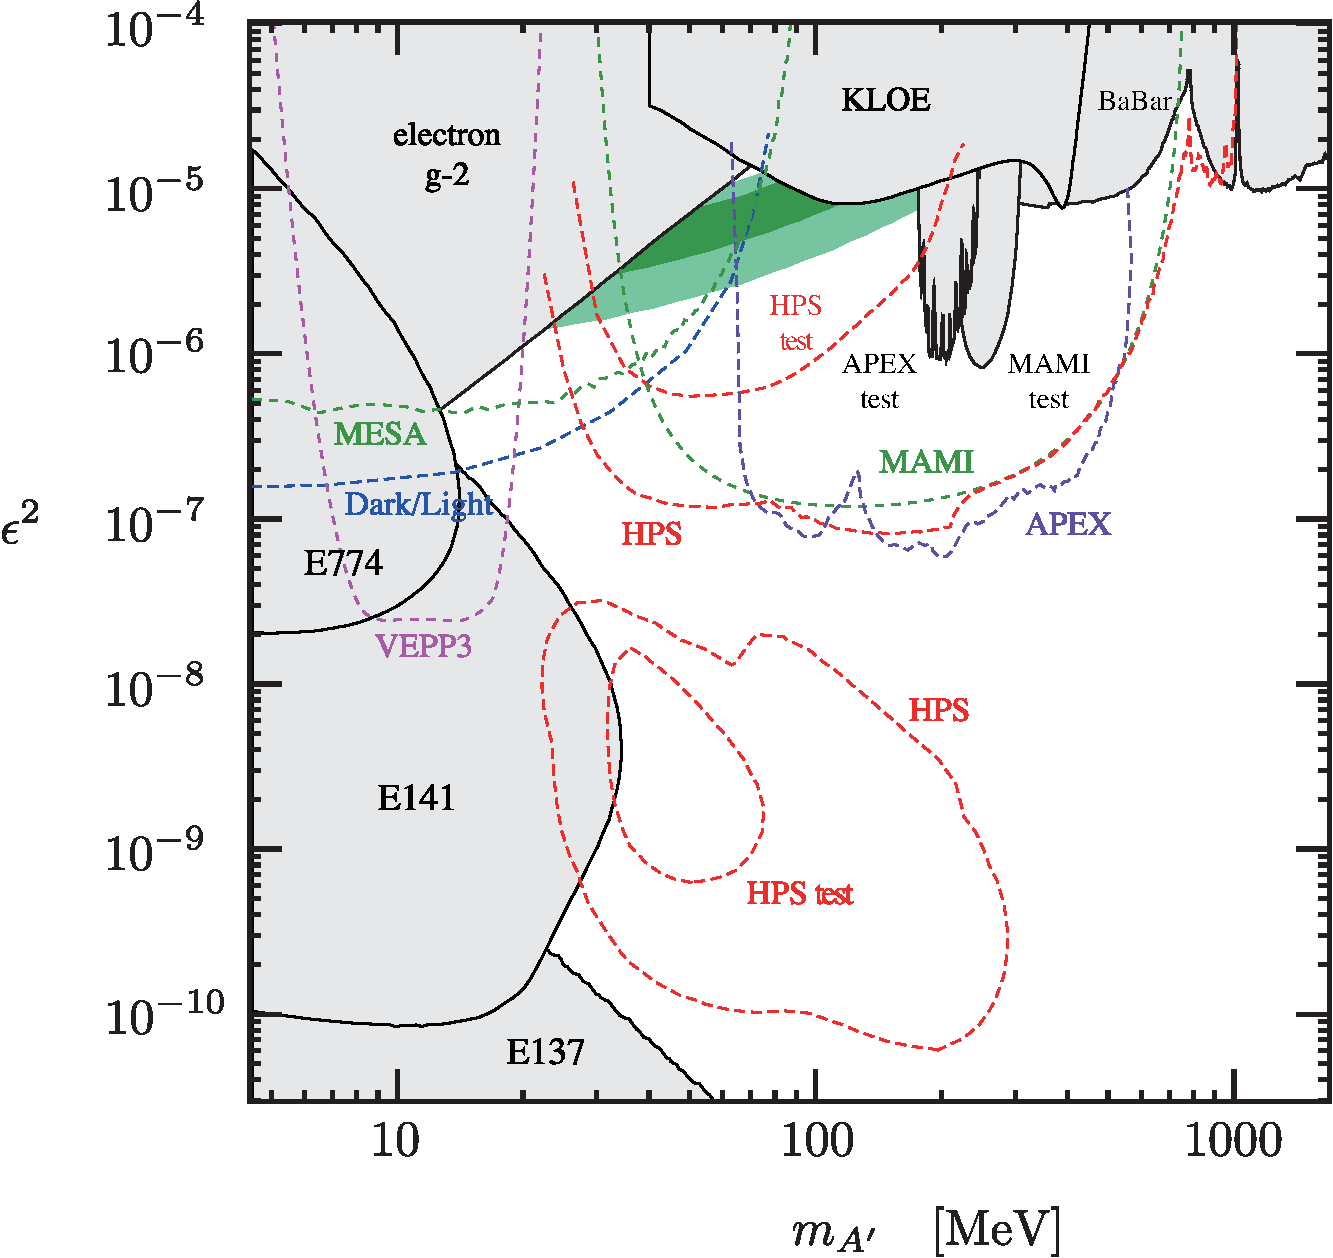
\includegraphics[width=0.7\textwidth]{limit_g-2_electron.pdf} 
\caption{ Existing constraints on heavy photons ($A'$). 
Shown are existing 90\% confidence level limits from the beam dump experiments 
E137, E141, and E774~\cite{Bjorken:2009mm,Bjorken:1988as,Riordan:1987aw,Bross:1989mp} 
the muon anomalous magnetic moment $a_\mu$~\cite{Pospelov:2008zw},  
KLOE~\cite{Collaboration:2011zc}, 
the test run results reported by APEX~\cite{Abrahamyan:2011gv} and MAMI~\cite{Merkel:2011ze}, 
an estimate using a BaBar result~\cite{Bjorken:2009mm,Reece:2009un,Aubert:2009cp},
a constraint from supernova cooling~\cite{Bjorken:2009mm} (see also~\cite{Dent:2012mx}) and a constraint from electron anomalous magnetic moment \cite{endo:g2e}.
In the green band, the $A'$ can explain the observed discrepancy between the
calculated and measured muon anomalous magnetic moment~\cite{Pospelov:2008zw} 
at 90\% confidence level.
%Projected sensitivities are shown for the full APEX run~\cite{Essig:2010xa}, 
%DarkLight~\cite{Freytsis:2009bh}, and VEPP-3~\cite{Wojtsekhowski:2009vz}.  
%MAMI has plans (not shown) to probe similar parameter regions as these experiments. 
Several projected sensitivities are shown for HPS. Solid red shows the 2$\sigma$ limits from the full HPS experiment, assuming 3 months of running time at each of 2.2 GeV(200 nA) and 6.6 GeV (450 nA). The upper region corresponds to a resonance search, the lower to a combined resonance plus vertexing search. Dashed red shows the limits from 1 week of running the HPS Test Run at 2.2 GeV (200 nA). The dashed blue limits corresponds to 1 week of running the Test Run at 1.1 GeV (200 nA).  
%Existing and future $e^+e^-$ colliders like \babar, BELLE, KLOE, Super$B$, BELLE-2, and KLOE-2  can also probe large 
%parts of the parameter space for $\epsilon\gtrsim 10^{-4}-10^{-3}$ (not shown).  
}
\label{fig:hspaw-heavy-A'}
\end{figure*}
%%%%%%%%%%

\subsubsection{Heavy Photons and Dark Matter}

The possible role of heavy photons in the physics of dark matter~\cite{ArkaniHamed:2008qn,Pospelov:2008jd} has provided an urgent impetus to search directly for heavy photons.  Results from two classes of dark matter searches --- ``indirect'' searches for galactic dark matter annihilation and ``direct'' searches for dark matter scattering off nuclei --- have both been interpreted as potential signals of dark matter interacting through a heavy photon.  Both fields have evolved in the last year, but not decisively.  New astrophysical constraints have altered the favored parameter space for dark matter annihilation into heavy photons, but a significant region remains viable, and this overlaps considerably with the projected sensitivity of HPS.  The motivation to test these theories of dark matter in a controlled laboratory experiment therefore remains strong.    Several direct-detection experiments have published conflicting bounds on dark matter scattering, and putative signals.  The physics of heavy-photon-mediated dark matter interaction was presented at some length in the proposal to PAC 37.  Here we briefly summarize the status of dark matter and the case for its interactions with heavy photons,  then discuss new observational constraints and theoretical developments.

The concordance model of big bang cosmology --- the Lambda Cold Dark Matter ($\Lambda$CDM) model --- explains all observations of the cosmic microwave background, large-scale structure formation, and supernovae, see 
e.g.~\cite{LambdaCDMData}. This model suggests that Standard Model particles make up only about 4\% of the energy density in the Universe, while ``dark energy'' and ``dark matter'' make up 74\% and 22\%, respectively, of the Universe's energy density. The concordance model does not require dark matter to have any new interactions beyond gravity with Standard Model particles. However, an intriguing theoretical observation, dubbed the ``WIMP miracle'', suggests that dark matter does have new interactions. In particular, if dark matter consists of ~10 GeV to 10 TeV particles interacting via an electroweak-strength force (weakly interacting massive particles or WIMPs), they would automatically have the right relic abundance consistent with the $\Lambda$CDM model.

If dark matter does interact with ordinary matter, it can interact in at least two ways: dark matter particles in the Milky Way Galaxy (and other bound astrophysical systems) can annihilate into visible matter, which could be detectable as energetic cosmic rays and/or gamma rays at Earth (indirect detection).  Dark matter passing through Earth can also scatter off nuclear targets, causing the target to recoil.  This recoil is observable in radio-pure detectors with sufficiently low background rates of nuclear recoil (direct detection).  

The satellites PAMELA \cite{Adriani:2008zr} and Fermi \cite{Ackermann:2010ij}, the balloon-borne detector ATIC \cite{Chang:2008aa}, the ground-based Cherenkov telescope HESS \cite{Aharonian:2008aa,Aharonian:2009ah}, and other experiments have all reported an excess in the cosmic-ray flux of electrons and/or positrons above backgrounds expected from normal astrophysical processes.  The evidence for this excess has only grown, with new measurements of the cosmic-ray electron flux by PAMELA \cite{Adriani:2011xv} and confirmation by Fermi of the positron excess \cite{FermiLAT:2011ab}.  It is expected that results from AMS-II will eventually shed more light on the spectrum of these excess cosmic-rays.  However, the origin of these excess positrons and electrons remains unknown.  It may plausibly arise from any of three possibilities: pair creation in nearby pulsars, acceleration in supernova shocks, or dark matter annihilation or decay.

If the excess arises from dark matter annihilation, two features are incompatible with annihilation of ``conventional'' thermal WIMP dark matter charged under the Standard Model weak interactions, but compatible with an alternative explanation, namely that dark matter is charged under a new $U(1)'$ and annihilates into $A'$ pairs, which decay directly into electrons and positrons, and/or into muons that decay into electrons and positrons (see e.g. \cite{ArkaniHamed:2008qn,Pospelov:2008jd,Cirelli:2008pk,Cholis:2008qq,Cholis:2008wq}): 
\begin{itemize}
\item The annihilation cross-section required to explain the electron signal is $50-1000$ times larger than the cross-section favored for the ``WIMP miracle''.   This can be explained if dark matter interacts with an $\mathcal{O}$(GeV)-mass $A'$, which mediates a new moderate range force and enhances the annihilation rate at low velocities (the relative velocity of dark matter in the Galactic Halo, $v\sim 10^{-3} c$, is much lower than in the early universe, and the relative velocity in self-bound dark matter subhalos is lower still).  We refer the reader to \cite{Finkbeiner:2010sm,Slatyer:2011kg} for a recent discussion.
\item The PAMELA satellite did not see any anti-proton excess \cite{Adriani:2008zq}, which implies that, if dark matter annihilation is responsible for the positron/electron signals, it does not produce baryons.  This contradicts expectations for dark matter annihilating through Standard Model interactions, but is expected if dark matter decays into light $A'$, which (for $m_{A'}\lesssim$ GeV) are kinematically unable to decay into protons and anti-protons.
\end{itemize}

Important constraints on the dark matter interpretation of these excesses arise from dark matter annihilation in other astrophysical systems (including dwarf galaxies \cite{Ackermann:2011wa}, the outer Milky Way \cite{DiffuseGalactic}, Galactic Center (e.g. \cite{Papucci:2009gd,Hutsi:2010ai} and references therein), and distant galaxies \cite{Hutsi:2010ai,extragalactic} and clusters \cite{Huang:2011xr}), and in the epoch of atomic recombination in the early universe, which leaves an imprint in the cosmic microwave background radiation \cite{CMBrefs}. 
Unfortunately, the most sensitive of the astrophysical constraints are also quite dependent on numerous astrophysical uncertainties, including the gamma-ray background fluxes and the phase-space distribution of dark matter.  

The status of models with light mediators ($\lesssim 200$ MeV), the target region for HPS, is particularly difficult to assess, because small, self-bound ``subhalos'' of dark matter with low velocity dispersions can easily enhance annihilation signals, both locally and in other galaxies.  The enhancement from subhalos in distant galaxies strengthens constraints on $A'$ models.  On the other hand, local enhancement lowers the couplings needed to explain the Fermi and PAMELA excesses, and these lower couplings are in turn less constrained by other systems.  Many analyses neglect the possibility of local subhalos, thereby overstating their exclusions of light $A'$ models.

Fits to N-body simulations do appear to favor a significant local substructure component \cite{Pieri:2009je,Kistler:2009xf,Kamionkowski:2010mi} which, in light $A'$ models, would easily dominate the local cosmic-ray signal.
	
Accounting for substructure at the level suggested by e.g.~\cite{Kamionkowski:2010mi},  light-$A'$ regions easily avoid constraints from the CMB, galactic center, dwarf galaxies, and dark matter self-interaction (though improved measurements of the CMB by Planck could severely constrain even these scenarios)~\cite{Slatyer:2011kg}.   Constraints on dark matter annihilation in distant galaxies (which would give rise to a diffuse and isotropic gamma-ray signal over the entire sky) are potentially severe even for these light-$A'$ models, but subject to theoretical uncertainties of several orders of magnitude.  In summary, light-$A'$ models of dark matter annihilation are consistent with all other data, but their viability depends on aspects of the dark matter distribution that are not yet reliably understood.

 The search for dark-matter-nuclear scattering has also seen considerable developments recently, but remains equally ambiguous.  Three experiments have reported excesses that \emph{may} be attributable to dark matter: DAMA/Libra \cite{Bernabei:2010mq}; CoGeNT \cite{Aalseth:2010vx}, which also reported an annual modulation signal \cite{Aalseth:2011wp}, and CRESST \cite{Angloher:2011uu}.   While these experiments' signals are most readily attributed to light dark matter ($\sim 10$ GeV), results from CDMS \cite{CDMS}, XENON10 \cite{Angle:2011th}, and XENON 100 \cite{Aprile:2011hi} appear to exclude the same parameter regions.  Some model parameter space remains moderately consistent with all of these results \cite{Kelso:2011gd}.  Though the evidence for light dark matter is controversial, it does raise a puzzle: dark matter with such low masses and high couplings cannot easily interact through Standard Model forces (such as $Z$ exchange), without being excluded by measurements of the total $Z$ width at LEP. If indeed dark matter is light, then it seems most likely to interact through a new mediator, a possibility that HPS will probe in the case of an $A'$.

\subsubsection{Heavy Photons and Muon $g-2$}

Besides being theoretically natural and having a possible connection to dark matter, an $A'$ could explain the discrepancy between the measured and 
calculated value of the anomalous magnetic moment of the muon $(a_\mu=g-2)$~\cite{Pospelov:2008zw}.  
This long-standing puzzle has several possible resolutions, but among the simplest new physics explanations
is the existence of a new force mediator that couples to muons, like the $A'$.  The contribution to $a_\mu$ of the $A'$ 
is like that of the photon, but suppressed by the mixing parameter $\epsilon^2$ and dependent on the $A'$ mass.  
The green region in Fig.~\ref{fig:hspaw-heavy-A'} is the 2$\sigma$ band in which the $A'$ can 
explain the discrepancy.  This is an intriguing region, which the HPS experiment will probe.  

\subsection{Update on Experimental Status}

The most recent (as of October 2012) comprehensive update summarizing the experimental status of $A'$ searches 
can be found in the presentations and summary talk of the Frascati ``Dark 2012'' workshop~\cite{Dark2012}.
All relevant measurements and constraints, as of this workshop, are included in Fig.~\ref{fig:hspaw-heavy-A'}.
One important change relative to a year ago is that an improved measurement of $g-2$ of the electron
has slightly reduced the range of allowed parameter space (on the low mass range) for an $A'$ to explain the $g-2$ of the muon 
discrepancy~\cite{endo:g2e}. 
Additionally, searches for $A'$s in rare $\phi$ decays at KLOE and rare $\pi^0$ decays at WASA have slightly reduced 
the allowed parameter space on the high mass range~\cite{rarek}. 
An ongoing search in the $e^+e^-$ spectrum of data recently gathered by MAMI~\cite{Merkel:2011ze} should also 
be sensitive to the $A'$ mass range explored by KLOE, but with sensitivity down to roughly $\epsilon\sim 10^{-3}$. 
Finally, improved theoretical calculations and modeling of the experimental acceptance have led to slightly revised constraints on the 
$A'$ parameter space from past beam dump experiments sensitive to $A'$ production and decay to $e^+e^-$ pairs~\cite{andreas}.


\subsection{HPS physics with True Muonium}

Positronium and muonium, bound states of $(e^+ e^-)$ and $(\mu^+ e^-)$ pairs, respectively, have been
produced and studied \cite{Deutsch:1951zza,Friedman:1957mz,Hughes:1960zz}, but true muonium has not yet been 
detected (see e.g. \cite{Holvik:1986ty,ArteagaRomero:2000yh,Brodsky:2009gx,Bilenky:1969zd,Hughes:1971,Malenfant:1987tm,Karshenboim:1998we,Owen:1972,Jentschura:1997ma,Jentschura:1997tv,Karshenboim:1998am}. 
Together with tauonium $(\tau^+ \tau^-)$ and tau-muonium $(\tau^{\pm} \mu^{\mp})$, true muonium is among the most
compact pure QED systems. While $(\tau^+ \tau^-)$ and $(\tau^{\pm} \mu^{\mp})$ are difficult to detect since the $\tau$ has a
weak decay that competes with the QED decay, the $\mu$ is very long lived so that the decay of true
muonium is purely a QED process. 

The detection of true muonium would be a significant discovery and would constitute a further important test of QED.   
A number of applications of true muonium measurements have been highlighted in 
\cite{Brodsky:2009gx}, designed to exploit true muonium as a perturbative laboratory 
for QCD bound state physics. 
These include measuring dissociation cross-sections as a function of energy and lifetimes of the various states. 
More speculatively, the discrepancy between theory and experiment for $g-2$ of the muon~\cite{Bennett:2006fi} and the discrepant measurement of
the charge radius of the proton using muon bound states~\cite{Pohl:2010zza} suggest that further measurements of 
muon properties would be useful to resolve these puzzles. 

That HPS will be the first experiment capable of detecting True Muonium is straightforward to understand. 
The triplet True Muonium states $1^3S_1$, $2^3S_1$, and $2^3P_2$ all eventually decay 
to $e^+e^-$ final states, with lifetimes long enough to leave a detectable displaced vertex.
In that important respect, triplet True Muonium states behave just like A's. 
True Muonium production kinematics is a bit different. 
In HPS, True Muonium will be produced by electron scattering off the high-Z nuclear target. 
The so-called ``single-photon'' production mechanisms gives rise to True Muonium states with kinematic extremely similar to A's -- HPS will be most 
sensitive to these. The ``three-photon'' production mechanism, which is typically larger, gives rise to True Muonium with characteristically lower energy. 
 
In addition to primary production mechanisms, there are a variety of secondary mechanisms
that are important in targets thicker than $\sim0.01\%$ radiation lengths.
This was studied in some detail in \cite{Banburski:2012tk}, where it was 
shown that $1^3S_1$ excitations (in the target) are the main source of 
$2^3S_1$ and $2^3P_2$ production.
The $2S$ and $2P$ state are especially long-lived, so this finding
suggests that HPS may first discover these states as they will comprise 
a sizable fraction of the $e^+e^-$ decays with displaced vertex in the range of $\sim 1$ cm to several cm. 
The $1S$ state will be the main component of the decays in the region of  $\sim 1$ cm and below. 

\subsection{HPS Searches for Hidden Sectors}

As highlighted in the Intensity Frontier Workshop report \cite{Hewett:2012ns},
a well-motivated class of beyond the Standard Model scenarios include new particles that interact
indirectly or very weakly with Standard Model matter (hidden sectors), possibly associated with dark matter. 
Low-energy and high-intensity experiments offer an excellent tool for exploring these
possibilities, complementary to the ongoing efforts at high energy colliders. 

HPS is primarily desinged to look for new sub-GeV A's that decay into lepton pairs.
But if an A' is part of a larger hidden sector, as is often assumed in the literature, 
some fraction of the decays could be more intricate.
For example, an A' might decay into hidden sector particles, which in turn may decay back into Standard Model lepton or photons.  
These decays would tyically have displaced vertices and multiple leptons or photons. The phenomenolgofy of a variety of such scenarios 
have been considered in \cite{Strassler:2006im, Essig:2009nc} (and references therein). 
Search strategies to look for more general decays of A's into hidden sector particles are actively being developed within HPS, 
and we comment in more detail on this physics opportunity in section 3.3.

%%%%%%%Additional References to Add%%%%%%%%%%%%




\clearpage


\section{Proposed Measurements}
\label{sec:measurements}

The primary goal of the proposed experiment is to search for a heavy photon (dark photon) in the mass range from 20 MeV to 1000 MeV in at least two settings of beam energy 2.2 GeV and 6.6 GeV. 
HPS  ultimately relies upon the precision measurement of two quantities: the invariant mass of the A$^\prime$ decay products and the position of the decay vertex. By placing a tracking and vertexing detector immediately downstream of the target inside an analyzing magnet, the complete kinematic information required for A$^\prime$ reconstruction can be obtained from a single system, whose proximity to the target naturally maximizes the acceptance of a relatively compact detector and provides excellent momentum and vertexing resolution. A finely segmented, fast electromagnetic calorimeter, just downstream of the tracker,  provides a powerful high rate trigger, identifies electrons, and augments  the electron energy measurement. Behind the ECal a muon system consisting of four planes of scintillator hodoscopes sandwiched between iron absorbers will be positioned. The muon system will provide a trigger for ($\mu^+\mu^-$) detection and will be used for muon identification. It will extend the search for high mass A$^\prime$ in di-muon decay mode where electromagnetic backgrounds are much reduced. Very high rate data acquisition systems, for the tracker, Ecal and muon system, make it possible to trigger and transfer data at $10$s of kHz, and run with negligible dead time.

The HPS experiment also has the potential to discover ``true muonium'', a bound state of a $\mu^+ \mu^-$ pair and to search for non-minimal hidden sector final states.  

HPS plans to execute the full experiment in two phases. The first phase will start with a commissioning run in 2014 which will include data taking at 1.1 and 2.2 GeV beam energies. More extensive data taking will continue in 2015, with runs at 2.2 and 6.6 GeV. This first phase will use about one sixth of the total beam time that HPS has requested, roughly 4 weeks on the floor at each of 2.2 and 6.6 GeV, which, assuming 50\% combined efficiency for the accelerator and detector, corresponds to one month total of (perfect) run time. The second phase of HPS running, which will occur in 2016 and beyond, will use the additional run time to extend the search for heavy photons to the largest possible region of parameter space, and study the properties of true muonium in detail.

\subsection{Search for the heavy photon}
\def \ap {A^\prime}
\def \map {m_{A^\prime}}
\def \thap {\theta_{A^\prime}}
%\subsubsection{Search for a Heavy Photon}
\label{sec:apsignal}

\begin{figure}
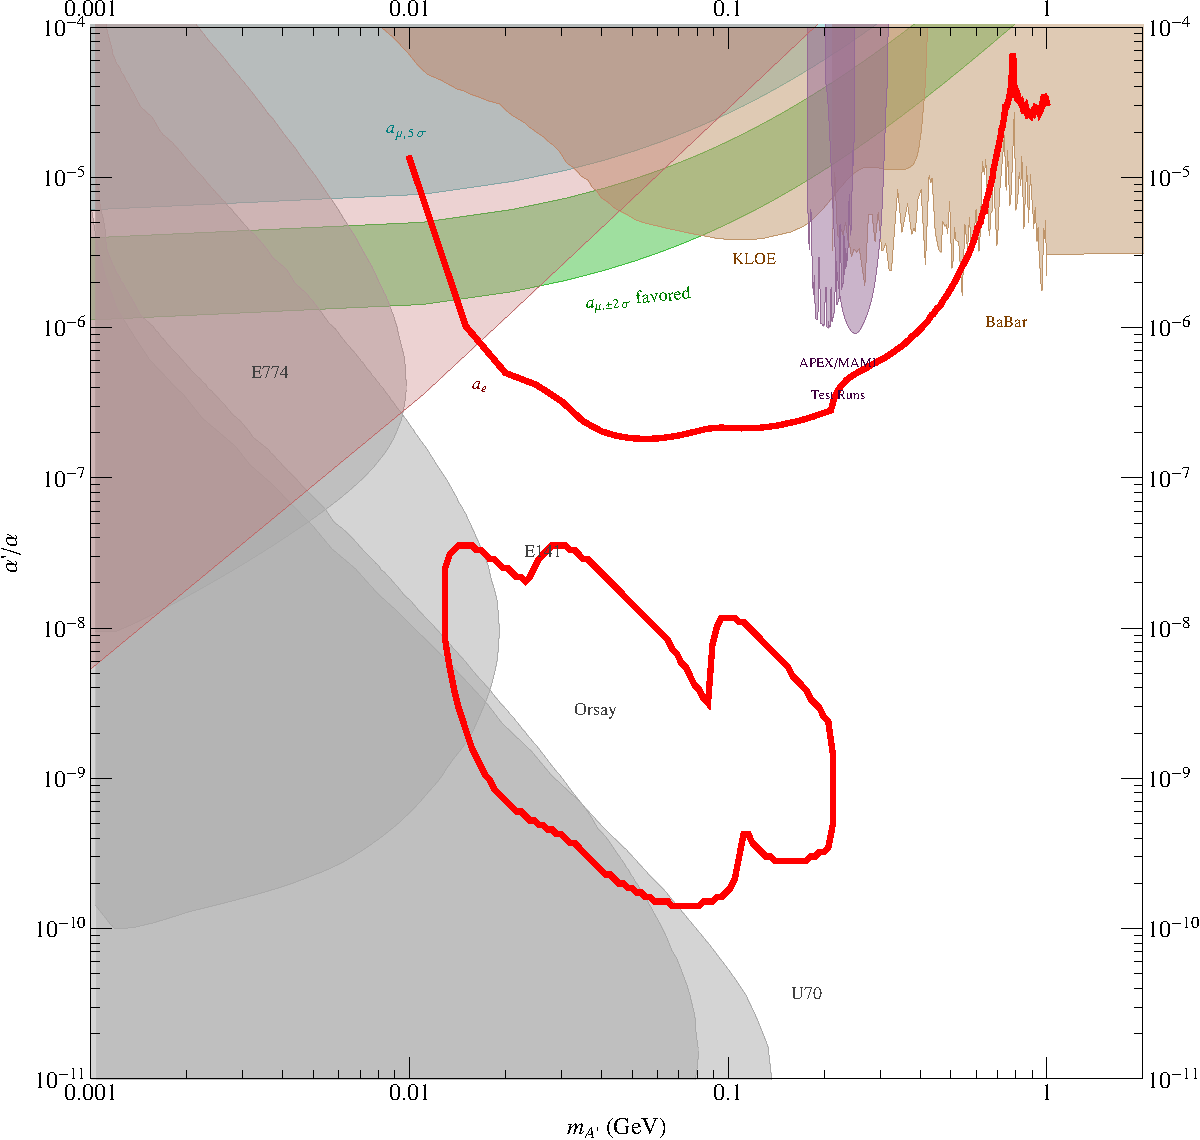
\includegraphics[width=0.9\textwidth]{measurements/HPS-Proposal2014-SimpleReach.pdf}
\caption{Expected mass vs coupling parameter space reach  full 2014-2015 running (solid red). Red line contour corresponds to 1 week of beam time at 1.1 GeV, and 3 weeks of beam time at 2.2 GeV and 6.6 GeV.}
\label{fig:reach}
\end{figure}

The expected in the first phase of the HPS is shown in Figure \ref{fig:reach}. The reach in mass-coupling parameter space is calculated using the simulated detector response as shown in Section \ref{sec:performance}.  The plot shows two distinct regions,  one at larger coupling corresponding to a purely bump-hunt region and another at lower coupling where the vertex of the $\ap$ decay is displaced.  



\begin{figure}
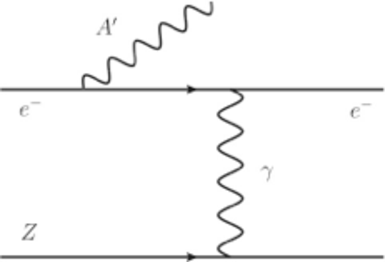
\includegraphics[scale=1]{measurements/Aprime-diagram.pdf}
\caption{Diagram of  $\ap$ production by bremsstrahlung off of an incoming electron scattering with an atomic nucleus.}
\label{fig:apdiagram}
\end{figure}

$\ap$ particles are generated in electron collisions on a fixed target by a process analogous to ordinary photon bremsstrahlung, see Figure \ref{fig:apdiagram}.  The rate and kinematics of $\ap$ radiation differ from massless bremsstrahlung in several important ways:
\begin{itemize}
\item  {\bf Rate}: The total $\ap$ production rate is controlled by $\alpha^3\epsilon^2 / m_{\ap}^2$.  
 Therefore, it is suppressed relative to photon bremsstrahlung by $\sim \epsilon^2 m_e^2/m_{\ap}^2$.  Additional suppression from small $\tilde{\chi}$  occurs for large $m_{\ap}$  or small $E_{beam}$, see \cite{Bjorken:2009mm} for details.
\item {\bf Angle}:  $\ap$ emission is dominated at angles $\theta_{\ap}$ such that the virtuality of the intermediate electron, $U$ (see definition in Eq.\ref{eq:u} in Appendix), is $U(x,\theta_{\ap})\lesssim 2 U(x,0)$ (beyond this point, wide-angle emission falls as $\theta_{\ap}^4$). Near its median value, the cutoff emission angle is
\begin{equation}
\theta_{\ap,max}\sim max\left(\frac{\sqrt{\map m_e}}{E_0},\left(\map/E_0\right)^{3/2}\right),
\end{equation}
which is parametrically smaller than the opening angle of the $\ap$ decay product, $\sim  \map/E_0$.  Although this opening angle is small, the backgrounds mimicking the signal dominate at even smaller angles.
\item {\bf Energy}:  $\ap$ bremsstrahlung is sharply peaked at $E_{A^\prime}/E_{beam}\approx 1$, where $U(x,0)$ is minimized.  When an $\ap$ is produced, it carries nearly the entire beam energy.  In fact, the median value of (1-x) is $\sim {\rm max}\left(\frac{m_e}{\map},\frac{\map}{E_0}\right)$.  
\item{\bf Lifetime} For the ranges of $\epsilon$ and $\map$ probed by this experiment, the mean decay length $l_0$ of the $\ap$ can be prompt or as large as tens of centimeters. All of the background decays promptly at the target.  
\end{itemize}
The  latter three properties are quite important in resolving signal events from the main backgrounds, as discussed
below.   More details of $\ap$ production and decay are given in Appendix \ref{app:ProdAndDecay}.

The irreducible background rates are given by the diagrams shown in Figure \ref{fig:radbhdiagram}. These trident events can be usefully separated into "radiative" diagrams (Figure \ref{fig:radbhdiagram} (a)), and "Bethe-Heitler" diagrams (Figure \ref{fig:radbhdiagram} (b)), that are separately gauge-invariant.  These QED tridents dominate the final event sample, so we consider their properties in some detail here.

\begin{figure}
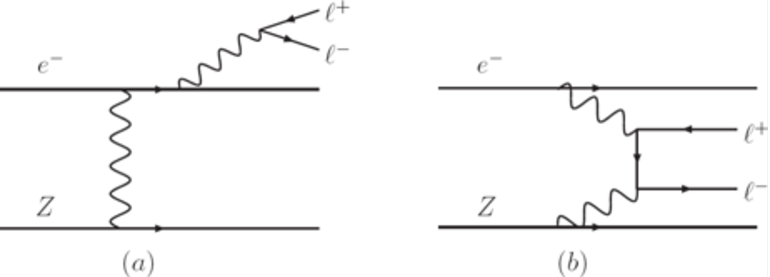
\includegraphics[scale=1]{measurements/rad-bh-diagrams.pdf}
\caption{Sample diagrams of (left) radiative trident ($\gamma^*$) and (right) Bethe-Heitler trident reactions that comprise the primary background to the $\ap\rarr l^+l^-$  search.}
\label{fig:radbhdiagram}
\end{figure}

The contribution from the radiative diagrams (Figure \ref{fig:radbhdiagram} (a)) alone is also useful as a guide to the behavior of $\ap$ signals at various masses. Indeed, the kinematics of the $A'$ signal events is identical to the distribution of radiative trident events restricted in an invariant mass window near the $A'$ mass. Moreover, the rate of the $A'$ signal is simply related to the radiative trident cross-section within the spectrometer acceptance and a mass window of width $\delta m$ by 
%\cite{4}
\begin{equation}
\frac{d\sigma\left(e^- Z \rarr e^- Z(\ap\rarr l^+l^-)\right)}{d\sigma\left(e^- Z \rarr e^- Z(\gamma^*\rarr l^+l^-)\right)}=\frac{3\pi\epsilon^2}{2 N_{eff}\alpha}\frac{\map}{\delta m}
\end{equation}
This exact analytic formula was also checked with a MC simulation of both the $\ap$ signal and the radiative trident background restricted to a small mass window $\delta m$, and we find nearly perfect agreement. Thus, the radiative subsample can be used to analyze the signal, which simplifies the analysis considerably.

 Although the Bethe-Heitler process has a much larger total cross-section than either the signal or the radiative trident background, it can be significantly reduced by exploiting its very different kinematics. In particular, the $\ap$ carries most of the beam energy while the recoiling electron is very soft and scatters to a wide angle. In contrast, the Bethe-Heitler process is not enhanced at high pair energies. Moreover, Bethe-Heitler processes have a forward singularity that strongly favors asymmetric configurations with one energetic, forward electron or positron and the other constituent of the pair much softer.
These properties are discussed further in the Appendix of [4], and illustrated in Figure \ref{fig:tridentkinematics}.

\begin{figure}
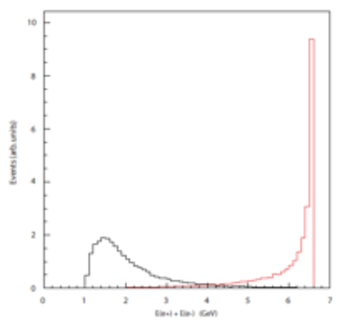
\includegraphics[scale=1.4]{measurements/rad-bh-energy.pdf}
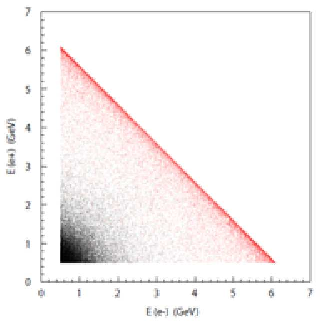
\includegraphics[scale=1.4]{measurements/E1vsE2.pdf}
\caption{ Left: The distribution of Bethe-Heitler background events (black) and $\ap$ signal events (red) as a function of the sum of the electron and positron energy. Note that the signal is peaked at high energies, while the background is peaked at much lower energies. Right: The distribution of the positron versus electron energy for Bethe-Heitler background events (black dots) and $\ap$ signal events (red dots). Note that in both plots neither the signal nor background events have been normalized to the correct number. In reality, the number of background events is much larger than the number of signal events. Also, note that the electron energy here refers to the energy of the electron produced in the reaction, not the recoiling beam electron.}
\label{fig:tridentkinematics}
\end{figure}



\subsection{Search for true muonium}

The proposed HPS experiment has the potential to discover ``true muonium'', a bound state of a
$\mu^+ \mu^-$ pair, denoted here by $(\mu^+ \mu^-)$. 
We expect that HPS will discover the 1S, 2S, and 2P true muonium bound states with its proposed run plan. 
The detection of these states should demonstrate the capability of the HPS experiment 
to identify rare separated vertex decays, and will provide a natural calibration 
tool for improving searches for heavy photons.
The $(\mu^+ \mu^-)$ atom is hydrogen-like, and so has a set of excited states characterized by a principal quantum number n. 
The binding energy of these states is E = $-1407$ eV/n$^2$. The $(\mu^+ \mu^-)$ ``atom'' can be produced by an electron beam incident on a target such 
as tungsten \cite{Holvik:1986ty,ArteagaRomero:2000yh}. 

With the existing proposal, HPS will search for true muonium
just as it does for heavy photons with separated vertices, requiring a vertex cut at about 1.5 cm to reject almost all
QED background events, then searching for a resonance at 2 m$_{\mu}$. An additional cut 
on the total energy of the $e^+e^-$ pair of $E_{e^-}+E_{e^+}> 0.8 \ E_{beam}$ will also be required
for triggering. 

Based on \cite{Banburski:2012tk}, the total production yield for 1S, 2S, and 2P (including secondary production)
leaving a target of thickness $t_b$(or larger) and satisfying the above requirements is,
\begin{equation}
N_{(\mu^+ \mu^-)} = 200 \left( \frac{I}{450 \ nA} \right) \left( \frac{t}{1 \ month} \right)
\end{equation}
%
where a beam energy E$_{beam} = 6.6$ GeV, and the nominal conditions
of 450 nA beam current for 2 weeks of beam-time ($\sim 2.6 \times 10^6$ s) on a single foil has been assumed.
The vertices near the cut of $1.5$ cm will be dominated by the 1S state, while 
a tail of vertices extending out beyond a few cm is dominated by 2S and 2P. 

Accounting for all the efficiencies associated with a separated vertex search, we would expect to see about 10--20 true muonium events in 2 weeks of $6.6$ GeV run
(we caution that the acceptance parameterization here is uncertain at the 50\% level).
The HPS experiment should be able to identify enough events to claim a discovery, and in addition, should be able to measure the mass of true muonium.  There are certainly other properties of true muonium that would be interesting to measure.  A measurement of the lifetimes would be interesting, as the lifetimes are sensitive to physics that couples to leptonic currents.  With enough statistics, it should be possible to perform a measurement of the lifetimes of the 1S, 2S, and 2P states; work is ongoing to investigate this possibility.  

\subsection{Other searches for hidden sector particles}
\label{sec:hidden_ex}

While the primary motivation for the HPS experiment is a search for $\ap$ decaying to lepton pairs, following Arkani-Hamed {\it et al.\/}\cite{ArkaniHamed:2008qn}, it is useful to explore the sensitivity of HPS is sensitive to other hidden sector particles, in particular those associated with Hidden Valley (HV) scenarios. As Strassler and Zurek\cite{Strassler:2006im} pointed out, HV scenarios provide many natural explanations of  the nature of Dark Matter. The recent discovery of a boson that seems to have the properties of the Higgs boson of the Standard model also brings an old problem to the fore: why is the Higgs mass so light compare to the Planck scale? Searches at the LHC for supersymmetric partners and other particles with Standard Model couplings have so far been unsuccessful, pushing the range of allowed masses for such particles higher and higher. HPS may be the first in a series of experiments that complement the energy frontier searches by looking for new, light particles that couple to the SM particles through new, very weak forces. Just as one should be ready for the  unexpected when exploring the energy frontier at the LHC, so should we be in exploring the coupling frontier at with HPS.

In a general HV scenario, the new fermions may be lighter than the $\ap$ and have their own QCD-like forces, which results in them forming hidden mesons and baryons. Some of these hidden particles may be part of the Dark Matter. These hidden mesons would decay into SM fermion pairs  either democratically or with mass-dependent branchings. 
\begin{figure}[ht]
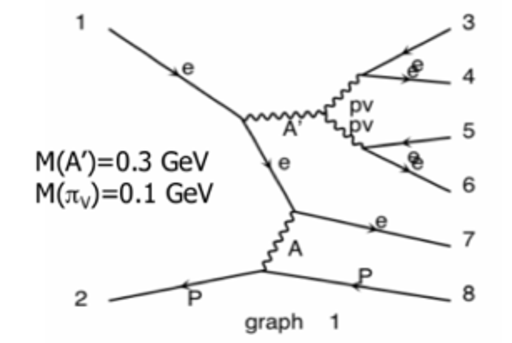
\includegraphics[scale=1]{measurements/multilepton-diagram.pdf}
\caption{Sample diagram of a non-Abelian hidden sector interaction.}
\label{fig:mldiagram}
\end{figure}
One interesting case is where the $\ap$ decays into a pair of dark mesons ($\pi_v$), which in turn promptly decay into electron pairs (see Fig \ref{fig:mldiagram}).  The high multiplicity of the typical final states makes an exclusive search for events such as these  difficult to trigger on, but it also reduces the background significantly by providing a number of new constraints and possible invariant mass bumps to search for and find.  Simulation studies are ongoing towards estimating the reach HPS has for such hidden mesons.  


%


\clearpage



\section{Description of the HPS setup}
\label{setup}

\subsection{Overview } 


HPS will utilize a setup located at the upstream end of the experimental Hall-B at Jefferson Lab. The setup will be based on a three-magnet chicane, the second dipole magnet serving as the analyzing magnet. The detector package will include silicon tracker, electromagnetic calorimeter and a muon detector. High luminosities are needed to search for heavy photons with small couplings and masses in the $20$ to $1000$ MeV range. Utilizing CEBAF�s essentially continuous duty cycle, the experiment can simultaneously maximize luminosity and minimize backgrounds by employing detectors with short live times and rapid readout. The HPS setup is designed to run with $> 200$ nA electron beam at energies from $1.1$ GeV to $6.6$ GeV impinging on a tungsten target of up to 0.0025 r.l. located at 10 cm upstream of the first layer of the tracker.

The HPS tracker consists of six double layer planes, 36 microstrip sensors in total. Placing the planes of the tracker in close proximity to the target means that the primary beam must pass directly through the middle of the tracking detector. This has necessitated that the sensors don't encroach on a �dead zone�, where multiple Coulomb scattered beam particles and radiative secondaries are bent into a horizontal plane, the so-called "wall of flame".  However, since the energy released in the decay of a low mass A$^\prime$ is small relative to its boost, the opening angle between decay daughters can be quite small. To maximize the acceptance for low mass A$^\prime$s, the vertical extent of the dead zone must be minimized and sensors placed as close as possible to the beam, so our design incorporates precision movers that can bring the silicon detectors  to the required positions. Since interactions of the primary beam with air or even helium at atmospheric pressure gives rise to low-momentum secondaries that generate unacceptable occupancies, we have chosen to place the entire tracking and vertexing system in vacuum, in the Hall B pair spectrometer's magnet vacuum chamber. Silicon microstrip sensors are used in the tracker/vertexer because they collect ionization in $10$�s of nanoseconds and produce pulses as short as $50-100$ ns. The sensors are read out continuously at $40$ MHz using the APV25 chip, developed for the CMS experiment at the LHC. Running high speed silicon module readout in vacuum further requires a vacuum compatible cooling system, and data and power vacuum feedthroughs. All these features are incorporated  in the design of apparatus, as described below, and has been tested in the May 2012 test run.


The electromagnetic calorimeter (Ecal) consists of 442 PbWO$_4$ crystals (reconfigured from the CLAS Inner Calorimeter) that are read out with APDs and amplifiers. The short  pulse widths allow ECal to run at very high rates. The Ecal data is digitized in the JLAB FADC250, a $250$ MHz flash ADC developed for the JLAB $12$ GeV Upgrade program.  The full analogue information from the FADCs coupled with the fine spatial information of the calorimeter is available to the trigger, which uses energy deposition, position, timing, and energy-position correlations to reduce the trigger rate to a manageable $\sim 30$ kHz. Like the tracker system, the electromagnetic calorimeter is split to avoid impinging on the �dead zone�. The beam and radiative secondaries pass between the upper and lower ECal modules, which are housed in the temperature-controlled enclosures, needed for stabilization of the energy calibration. 

The muon detection system will be installed behind the ECal that absorbs most of the electromagnetic background produced in the target. The remainder will be attenuated by the first absorber layer of the muon system. The muon system will consist of four double layers of scintillator hodoscopes sandwiched between iron absorbers. Light readout from scintillator strips will be done via wave-length shifting fibers embedded inside holes in the strips and photomultipliers. As in the case of ECal, muon system will be divided into two parts, beam up and beam down. There is a vacuum chamber between the two parts to allow the beam and radiated secondaries pass through. 

In the following, the various elements of the experiment are discussed in more detail, beginning with the beamline, continuing with the tracker/vertexer, electromagnetic calorimeter, muon system, data acquisition systems, trigger, and calibration system.
 
 


 \subsection{HPS beamline}
 \label{setup:beamline}
 
The Hall-B beam line, magnetic elements, beam profile monitors, and beam position and current monitors upstream of the HPS setup will be 
used as is (after slight modifications for 12 GeV). The only modification needed for the upstream part of the beam line is the addition of 
a collimator upstream of the Hall-B tagger magnet. The role of the collimator is to prevent the beam from directly hitting the Si-tracker in an 
event in which the high intensity beam can move up or down from its nominal position. The collimator, which  can consist of  a $1$ cm 
thick tungsten plate with different size oval holes (to match the beam profile), can be incorporated into the Hall-B photon tagger radiator ladder 
to provide vertical alignment. Horizontal alignment of the whole system will also be needed for fine tuning of the collimator position 
relative to the beam. Downstream of the HPS setup, there will be two beamlines, the electron beam line that will transport electron beam to the 
Hall-B electron beam dump, and a photon beam line that will transport the photon beam generated in the target to a photon beam dump mounted 
on the space frame. The electron beam will be transported in vacuum all the way through to the beam dump. Following the vacuum 
chamber in the last chicane dipole, the photon beam will go to the dump in Helium bag. There will be an H-corrector installed on the electron 
line after 
the HPS chicane to compensate any possible mis-steering of the beam in the chicane and to make sure that the electron beam stays on the 
original beamline to the dump. A YAG viewer will be used to monitor beam position just before the dump. The beam position on the dump monitor 
must stay unchanged before and after energizing the chicane.  
 
 \subsubsection{Layout of the HPS setup} 
 \label{setup:layout}
 
The HPS experiment will use the same three magnet chicane that was used for the CLAS Two Photon Exchange experiment (TPE). The layout of 
the beam line and the chicane is shown in Figure \ref{fig:ebeam}. The Hall B pair spectrometer magnet, an 18D36 (pole length $91.44$ cm, 
gap $45.72\times 15.24$ cm$^2$, max-field $1.5$ T), will serve as the analyzing magnet. The dipole field direction (Y) is perpendicular 
to the horizontal (XZ) plane. The Hall B ``Frascati'' H magnets (pole length $50$ cm, gap $21\times 8.25$ cm$^2$, max-field $1.2$ T) 
will be used as the first and the last dipoles of the chicane. The analyzing magnet will be operated at a $0.25$ T-m field for $1.1$ 
GeV, a $0.5$ T-m field for $2.2$ GeV, and a $1.5$ T-m field for $6.6$ GeV running. The two bending magnets will be set to  $0.125$ 
T-m, $0.25$ T-m, and $0.75$ T-m fields, respectively. The distance between the centers of the magnets will be about $50$ cm bigger than 
it was for the TPE run, to accommodate the muon system. The location of the analyzing magnet along the beam will be exactly the same  
as it was for the TPE run. 

The analyzing magnet will be displaced to beam left by $\sim 11$ cm in order to optimize the detector acceptance for e$^+$ 
and e$^-$, see Figure \ref{fig:ebeamt}.
 
 \begin{figure*}[!ht]
%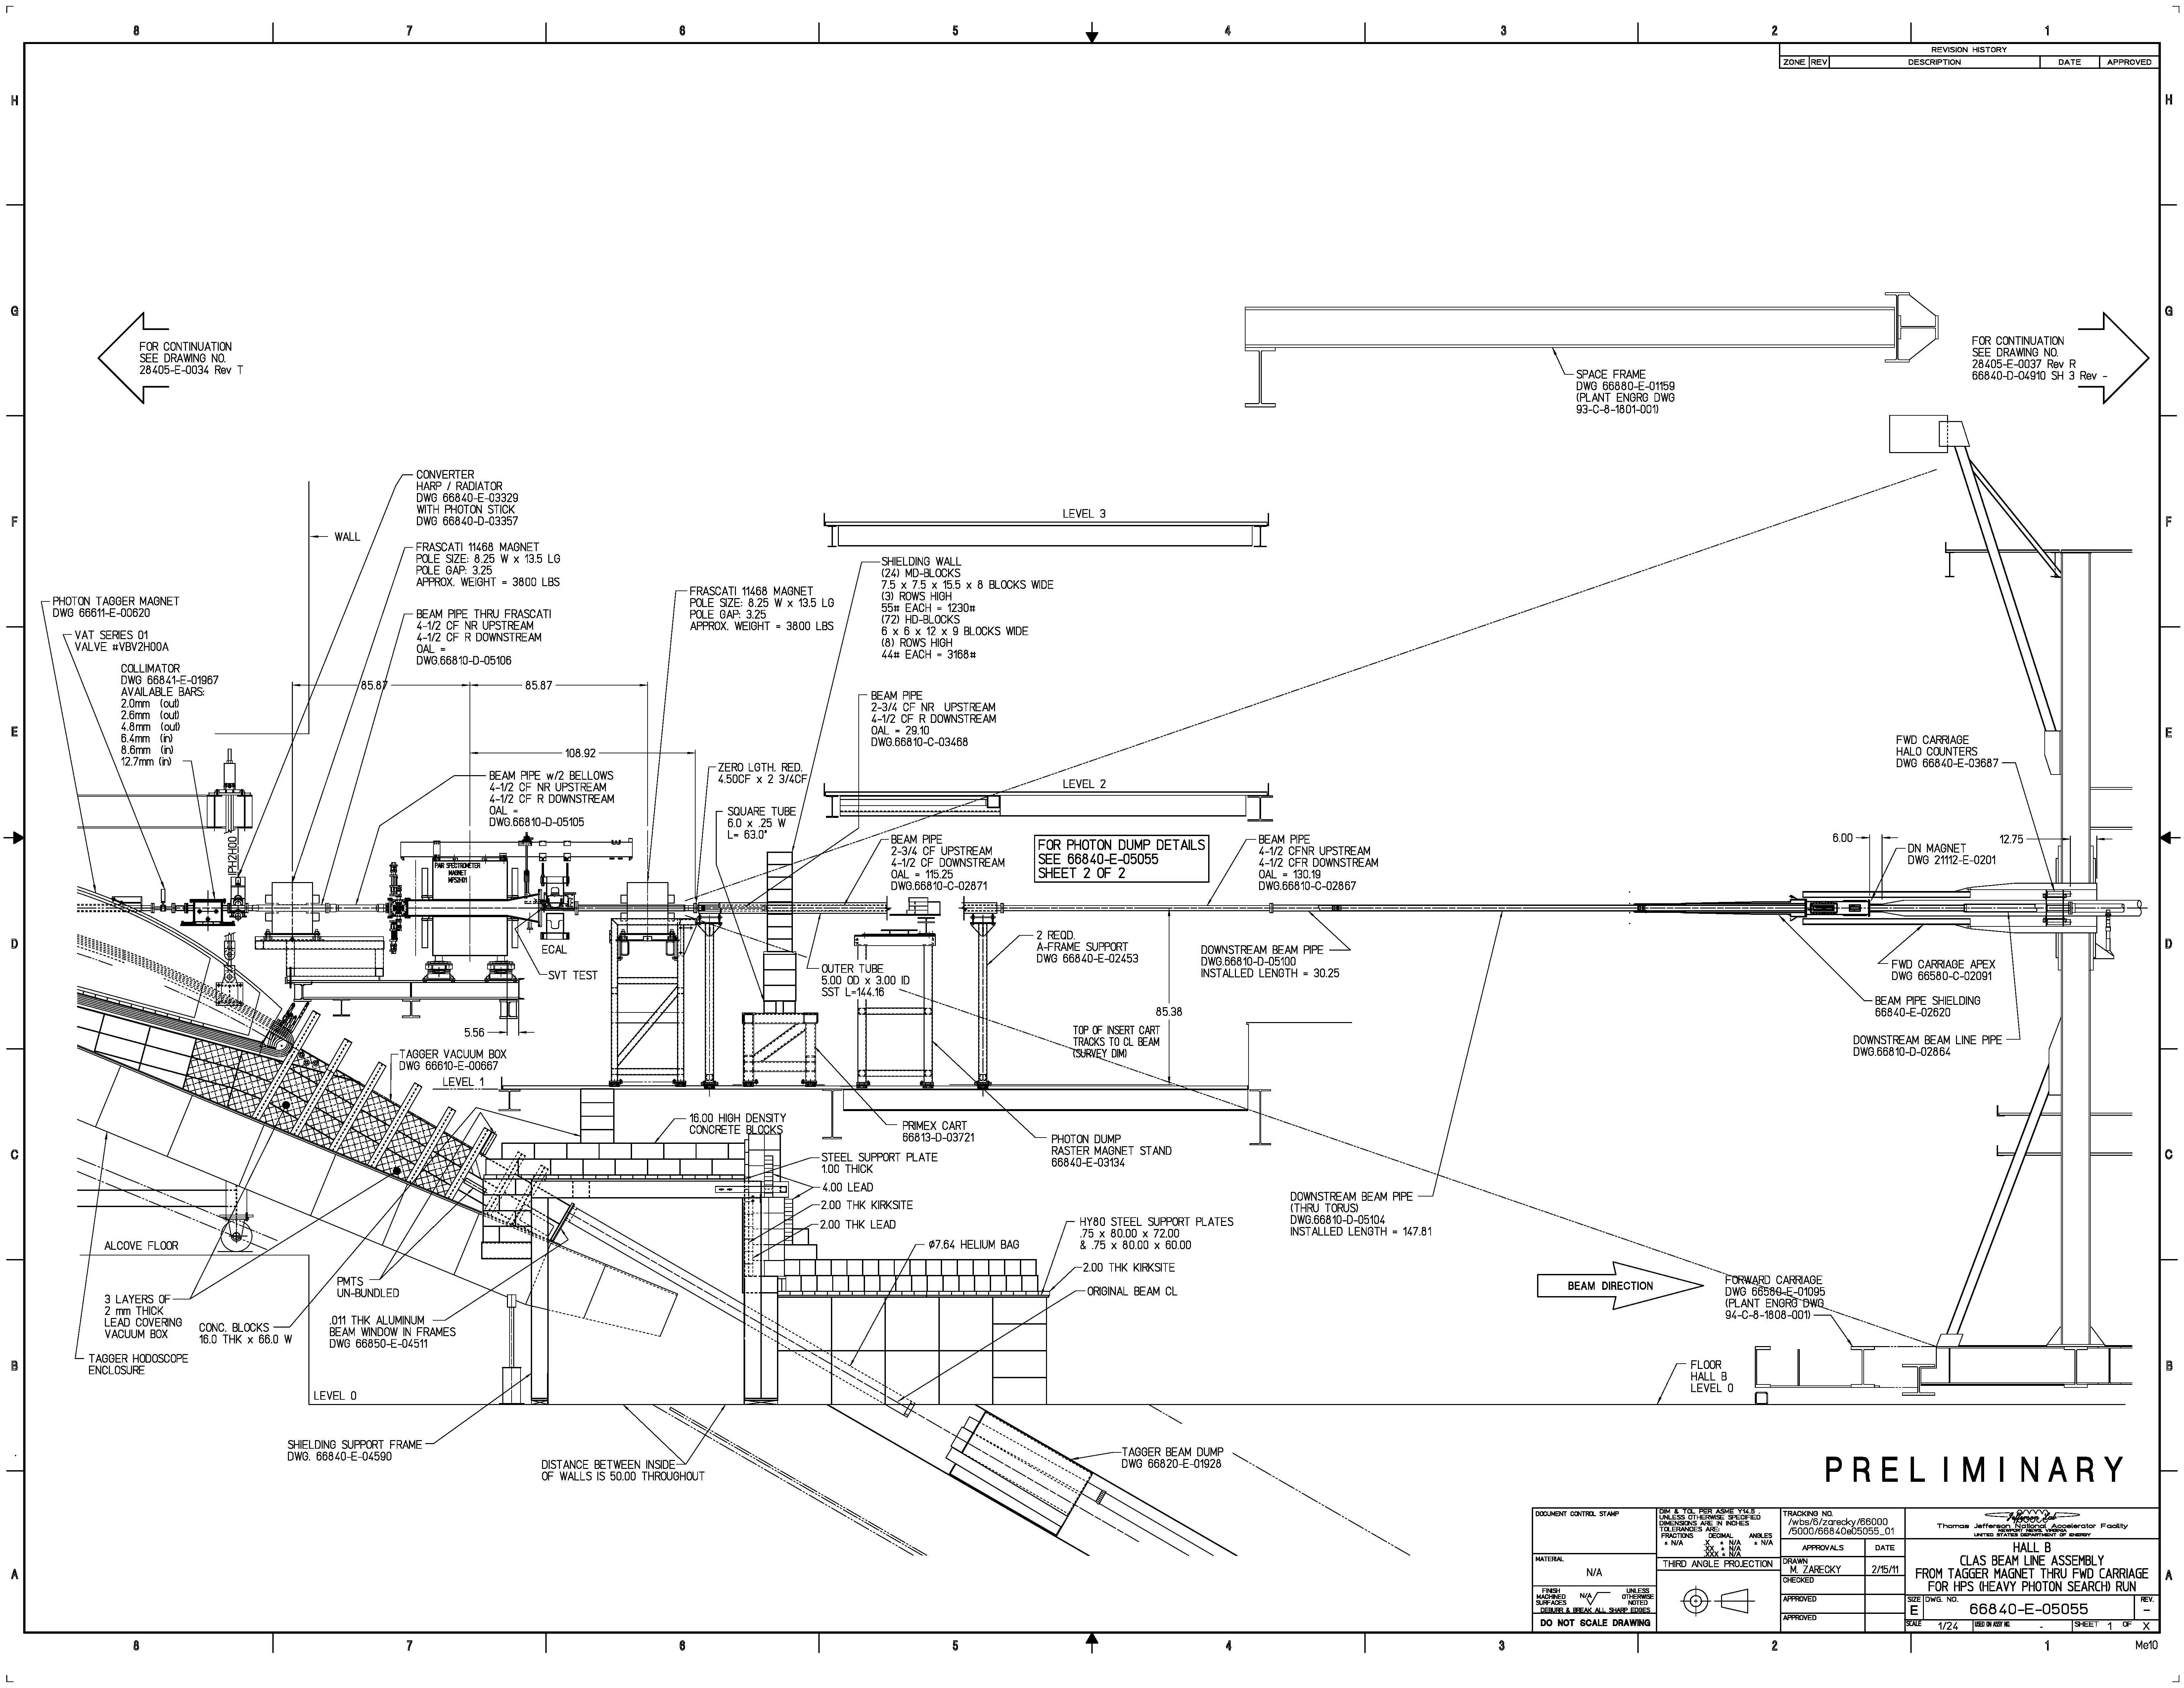
\includegraphics[scale=0.18]{beamline/05055-01_NT.pdf}
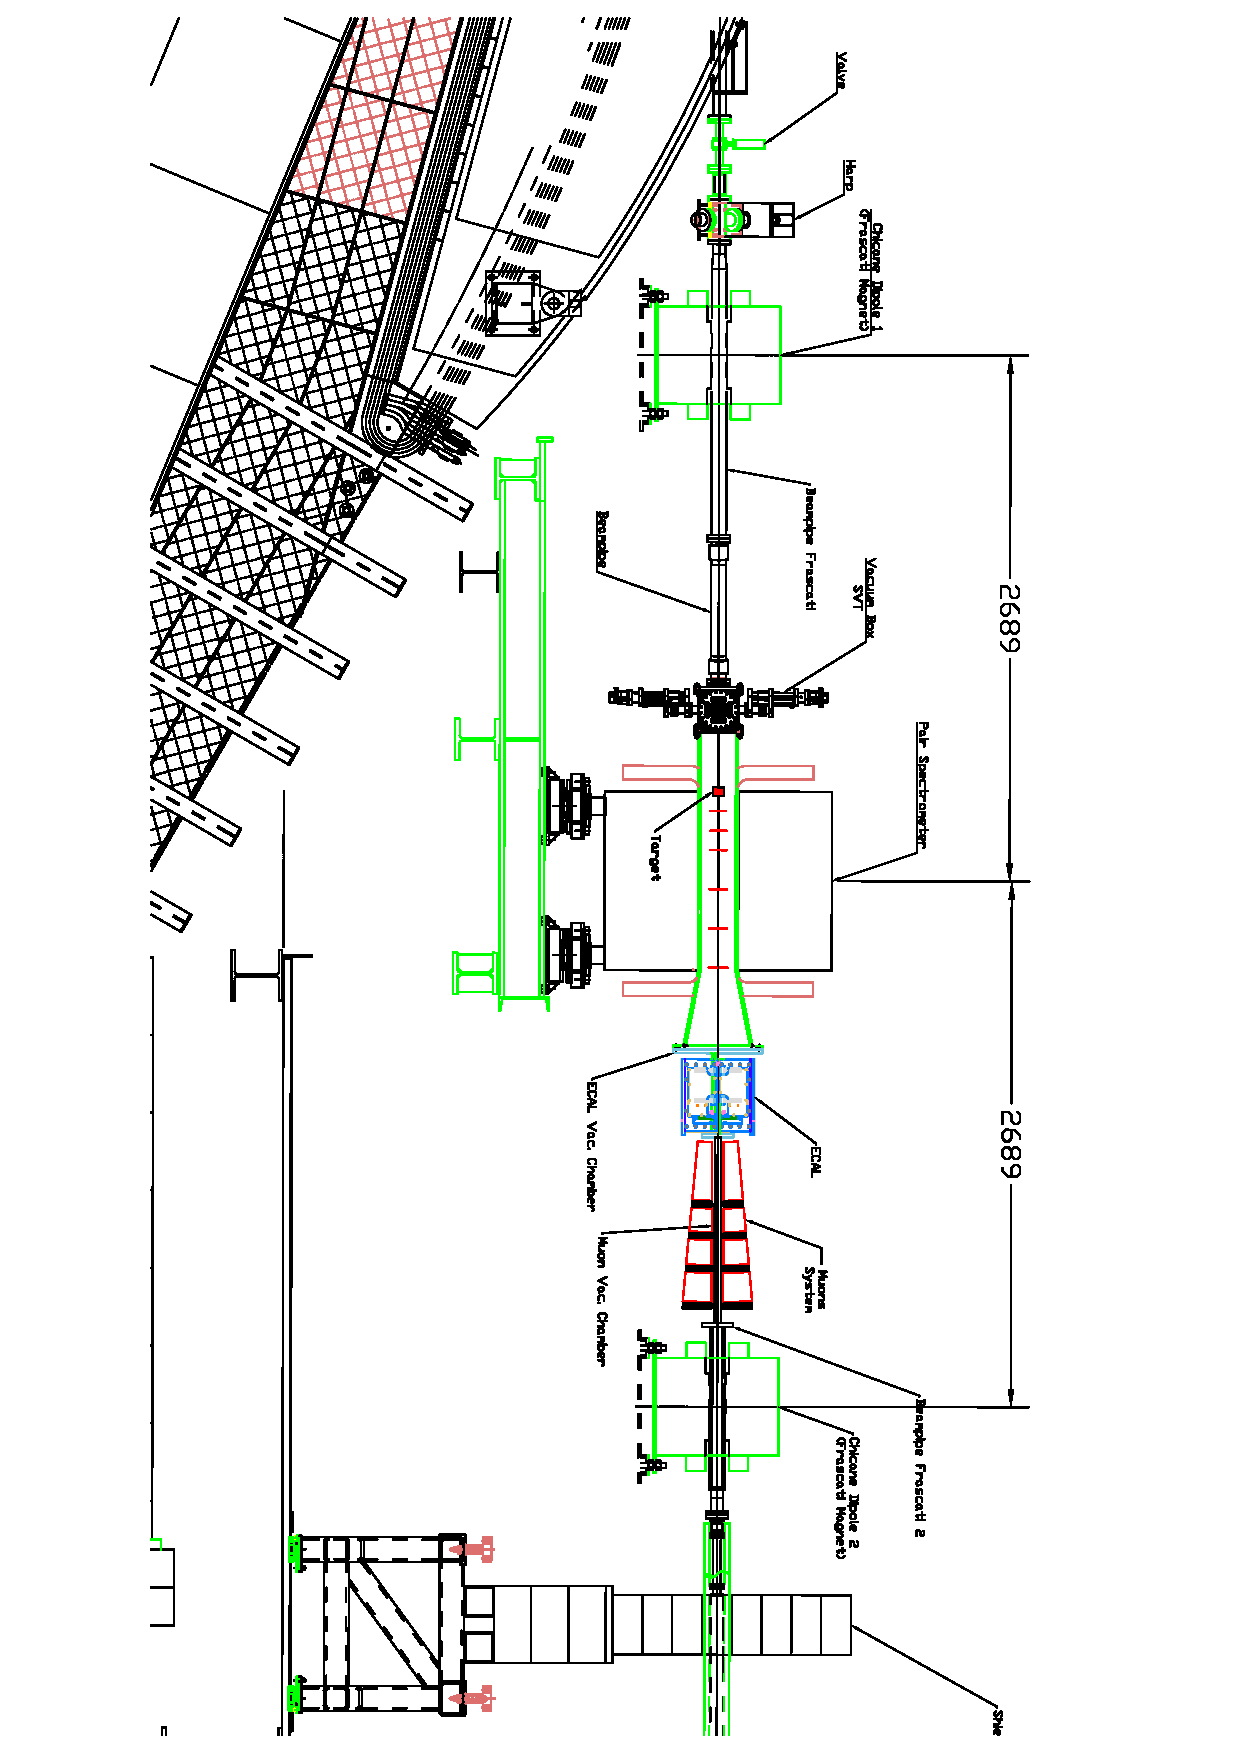
\includegraphics[angle=180, width=0.85\textwidth]{beamline/HPS12_66840e051XX_ELEV.pdf}
\caption{\small{Beam line configuration for the HPS test run with electron beams. The chicane configuration is similar to a previously run 
CLAS experiment.}}\label{fig:ebeam}
\end{figure*}

\begin{figure*}[htp]
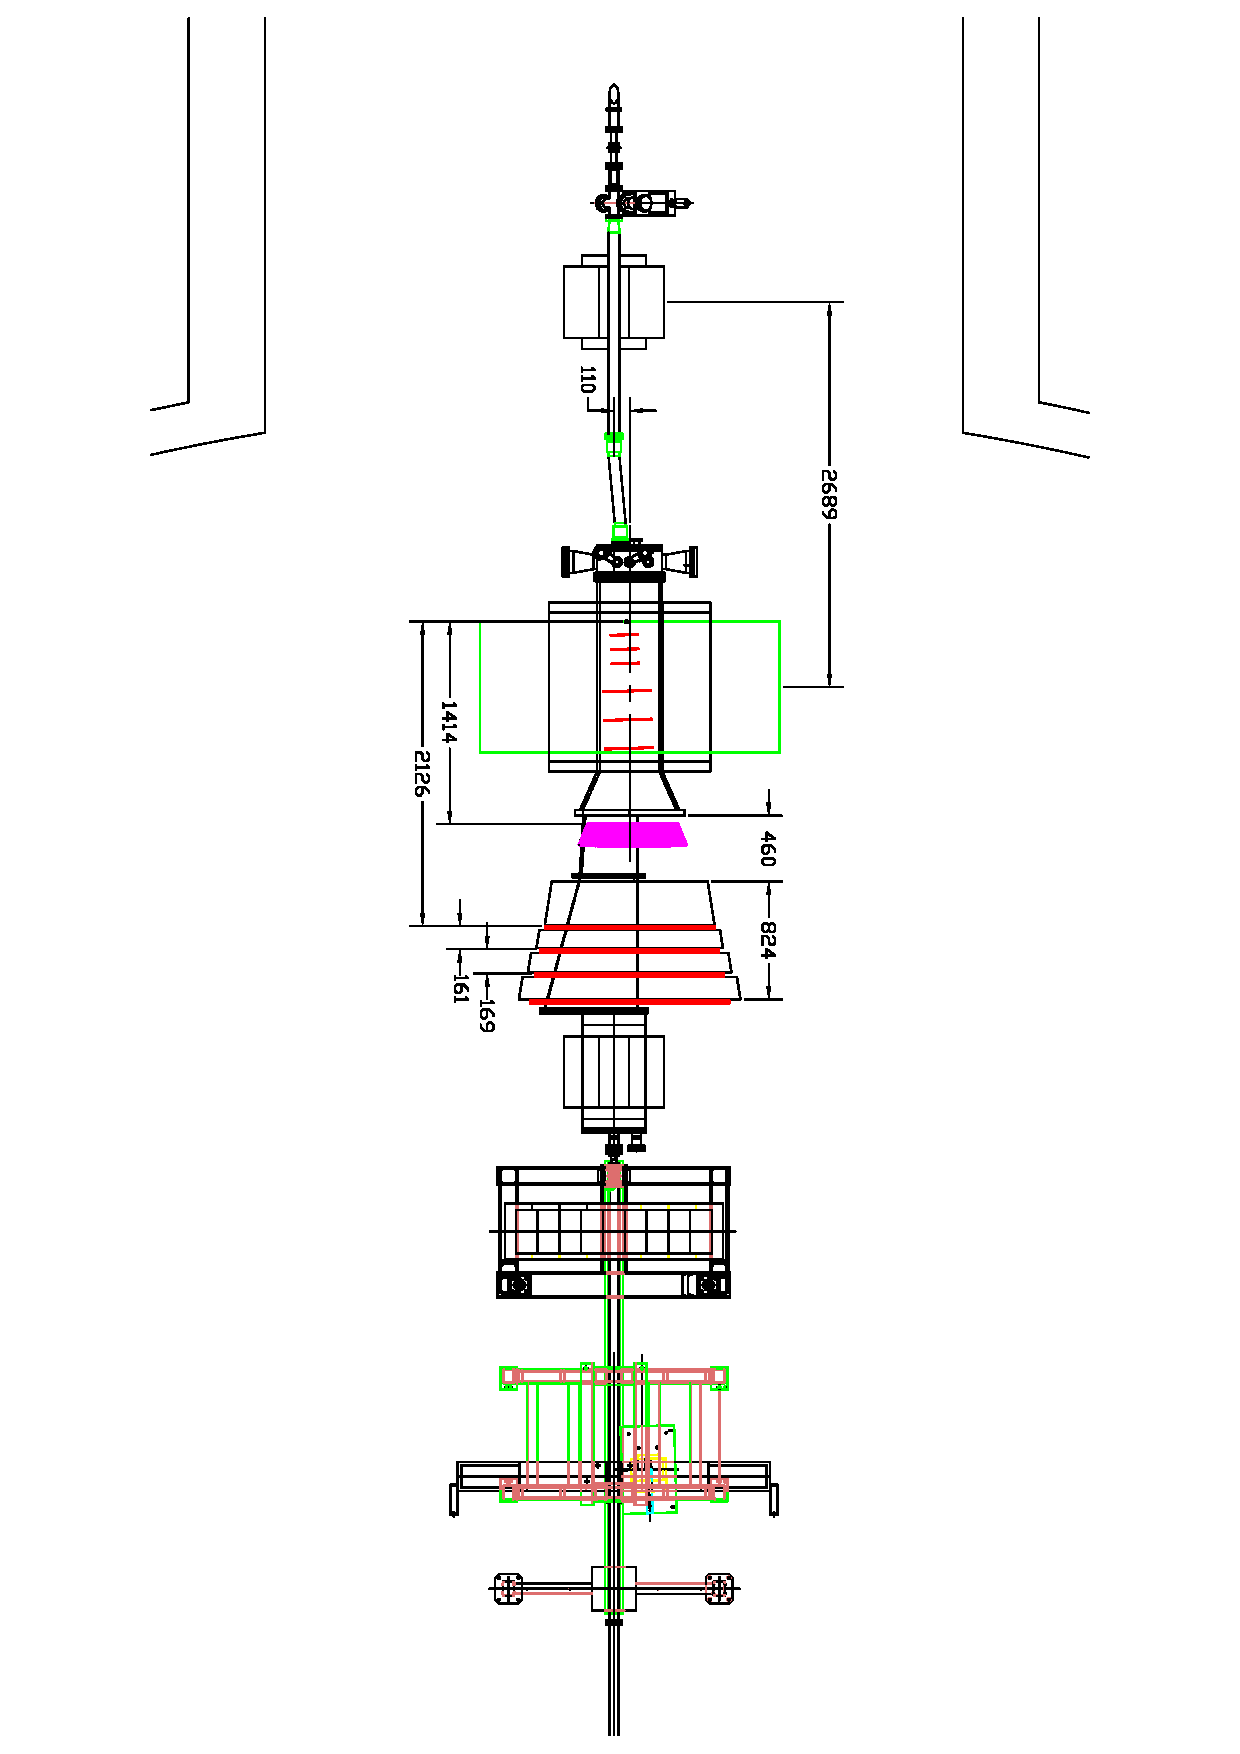
\includegraphics[angle=180., width=0.85\textwidth]{beamline/HPS12_66840e051XX_PLAN.pdf}
\caption{\small{Top view of the beam line configuration for the HPS test run with electron beams. The analyzing magnet is shifted by 4 inches 
(110 mm) to beam's left to get optimal acceptance for both $e^+$s and $e^-$s.}}\label{fig:ebeamt}
\end{figure*}

 
The HPS target is positioned at the upstream edge of the analyzing magnet's pole. The distance from the target to the first layer of the 
silicon tracker is $10$ cm, and to the face of the electromagnetic calorimeter $\sim 137$ cm. There is continuous vacuum for the electron 
beam throughout the entire setup ending in the Hall B electron beam dump. The Si-tracker and the target will be located inside the Hall-B 
pair spectrometer vacuum chamber. The SVT vacuum box is mounted on the upstream end of the analyzing magnet vacuum chamber to provide 
connections for the SVT motion system, the cooling system, power and signal cables, and the target motion system. The Ecal vacuum chamber 
is attached to the downstream end of the analyzing magnet vacuum chamber, above and below which are placed the Ecal modules. Downstream of 
the Ecal vacuum chamber, another vacuum chamber is attached, leading to the downstream chicane magnet.

The analyzing magnet, the Hall B pair spectrometer dipole, has its own power supply. The ``Frascati'' H magnets will use one common power 
supply and will be powered by the Hall B ``mini-torus'' power supply. There will be a shunt installed between the two ``Frascati'' magnets 
to allow independent small changes in currents on those two magnets if necessary (as it was done during the TPE experiment, although 
never used). Both power supplies are bipolar, so the magnets can be degaussed when needed. From available field map data at $900$ A, 
the$\int{Bdl}$ of Frascati H magnets along the path of the electron beam is $0.663$ T-m. The specified max current for these magnets 
is $950$ A. In order to get $0.75$ T-m an additional $10\%$ increase in field value will be needed. From initial evaluation of the 
magnet design and characteristics, it should not be a problem to run them at $10\%$ higher currents over their specified max current. 
If this is not possible, reducing the gap by $1/3$ inch can yield the desired $\int{Bdl}$. 

 
\clearpage

\subsubsection{Running Conditions} 
 
The HPS will use $\sim 1.1$ GeV, $\sim 2.2$ GeV, and $\sim 6.6$ GeV electron beams of up to $500$ nA incident on a thin tungsten (W) target. 
Operational experience (with 6 GeV machine) showed that the CEBAF beam is very clean, and is contained within $\pm 0.5$ mm with halo at the level 
of less than $10^{-5}$. It is expected that the beams from the 12 GeV machine will be of comparable quality, at least for up to 3-pass 
beams (up $\sim 6.6$ GeV), so the primary electron beam should cleanly pass through the ``dead zone'' gap of the HPS setup. 
 
For optimizing the vertexing performance and acquiring physics data, an asymmetric beam profile is desirable. Since the vertex resolution 
in the non-bend plane will be high, beam sizes of $<50 ~\mu$m in the Y direction are preferable. The momentum measurement will not benefit 
from small beam sizes in the X direction, and if the beam sizes in both dimensions are too small, the target foil will overheat. For these reasons the 
required beam sizes for HPS will be $\sigma_X \sim 250 \mu$m and $\sigma_Y < 50 \mu$m.
The HPS beam parameter requirements are presented in Table \ref{tb:beam}. 
 
 \begin{table}[!htb]
 \centering
 \begin{tabular}{|c|c|c|c|c|}
\hline
%Parameter & \multicolumn{3}{c|}{Requirement/Expectation} &Unit \\ \hline 
Parameter & \multicolumn{3}{c|}{Requirement} &Unit \\ \hline 
E & $1100$ & $2200$ & $6600$ & MeV \\ \hline
$\delta$E/E & \multicolumn{3}{c|}{$< 10^{-4}$} & \\ \hline 
Current & $< 200$ & $< 400$ & $< 500$ & nA \\ \hline
Current Instability & \multicolumn{3}{c|}{$< 5$} &\% \\ \hline 
$\sigma_x $& \multicolumn{3}{c|}{$< 300$ } & $\mu$m \\ \hline 
$\sigma_y$&\multicolumn{3}{c|}{$<50$} & $\mu$m \\ \hline
Position Stability & \multicolumn{3}{c|}{$< 30$} &$\mu$m \\ \hline
Divergence& \multicolumn{3}{c|}{$< 100$} & $\mu$rad \\ \hline 
Beam Halo ($> 5\sigma_Y$) & \multicolumn{3}{c|}{$< 10^{-5}$} & \\ \hline
 \end{tabular}
\caption{ Required beam parameters.} 
\label{tb:beam}
\end{table}

The B-line optics in the $6$ GeV era was checked using simulation and a beam test of the system. The optics program ELEGANT \cite{elegant} was 
used to determine the optimized B-line parameters needed to achieve an asymmetric beam size, $\sigma_X \approx 250 \mu$m and $\sigma_Y\approx 
20 \mu$m, at the HPS test run target location. 
Beam tests were conducted in Hall B to validate these optics simulations during the Two Photon Exchange experiment when $2.2$ GeV beam was 
available (February of 2011). Parameters were set for a beam profile of $\sigma_X \approx 300 ~\mu$m and $\sigma_Y\approx 10 \mu$m at the 
Hall B ``tagger'' beam profiler ($\sim 8$ meters upstream of the proposed HPS target location). Several beam profile scans with different 
scanner and data readout speeds were performed to check the beam stability and the systematics in the measurements. 
One of the scans is shown in Figure \ref{fig:profile_test}. As can be seen from the figure, the required profile can be reliably  achieved. 
Several scans performed over two hours resulted in a consistent and stable beam profile. Based on the width of the Y-profile, beam position 
stability is  $< 20 \mu$m. Note that any beam motion with more than 10 $\mu$m amplitude and faster than 1Hz is included in the scan.

\begin{figure*}[t]
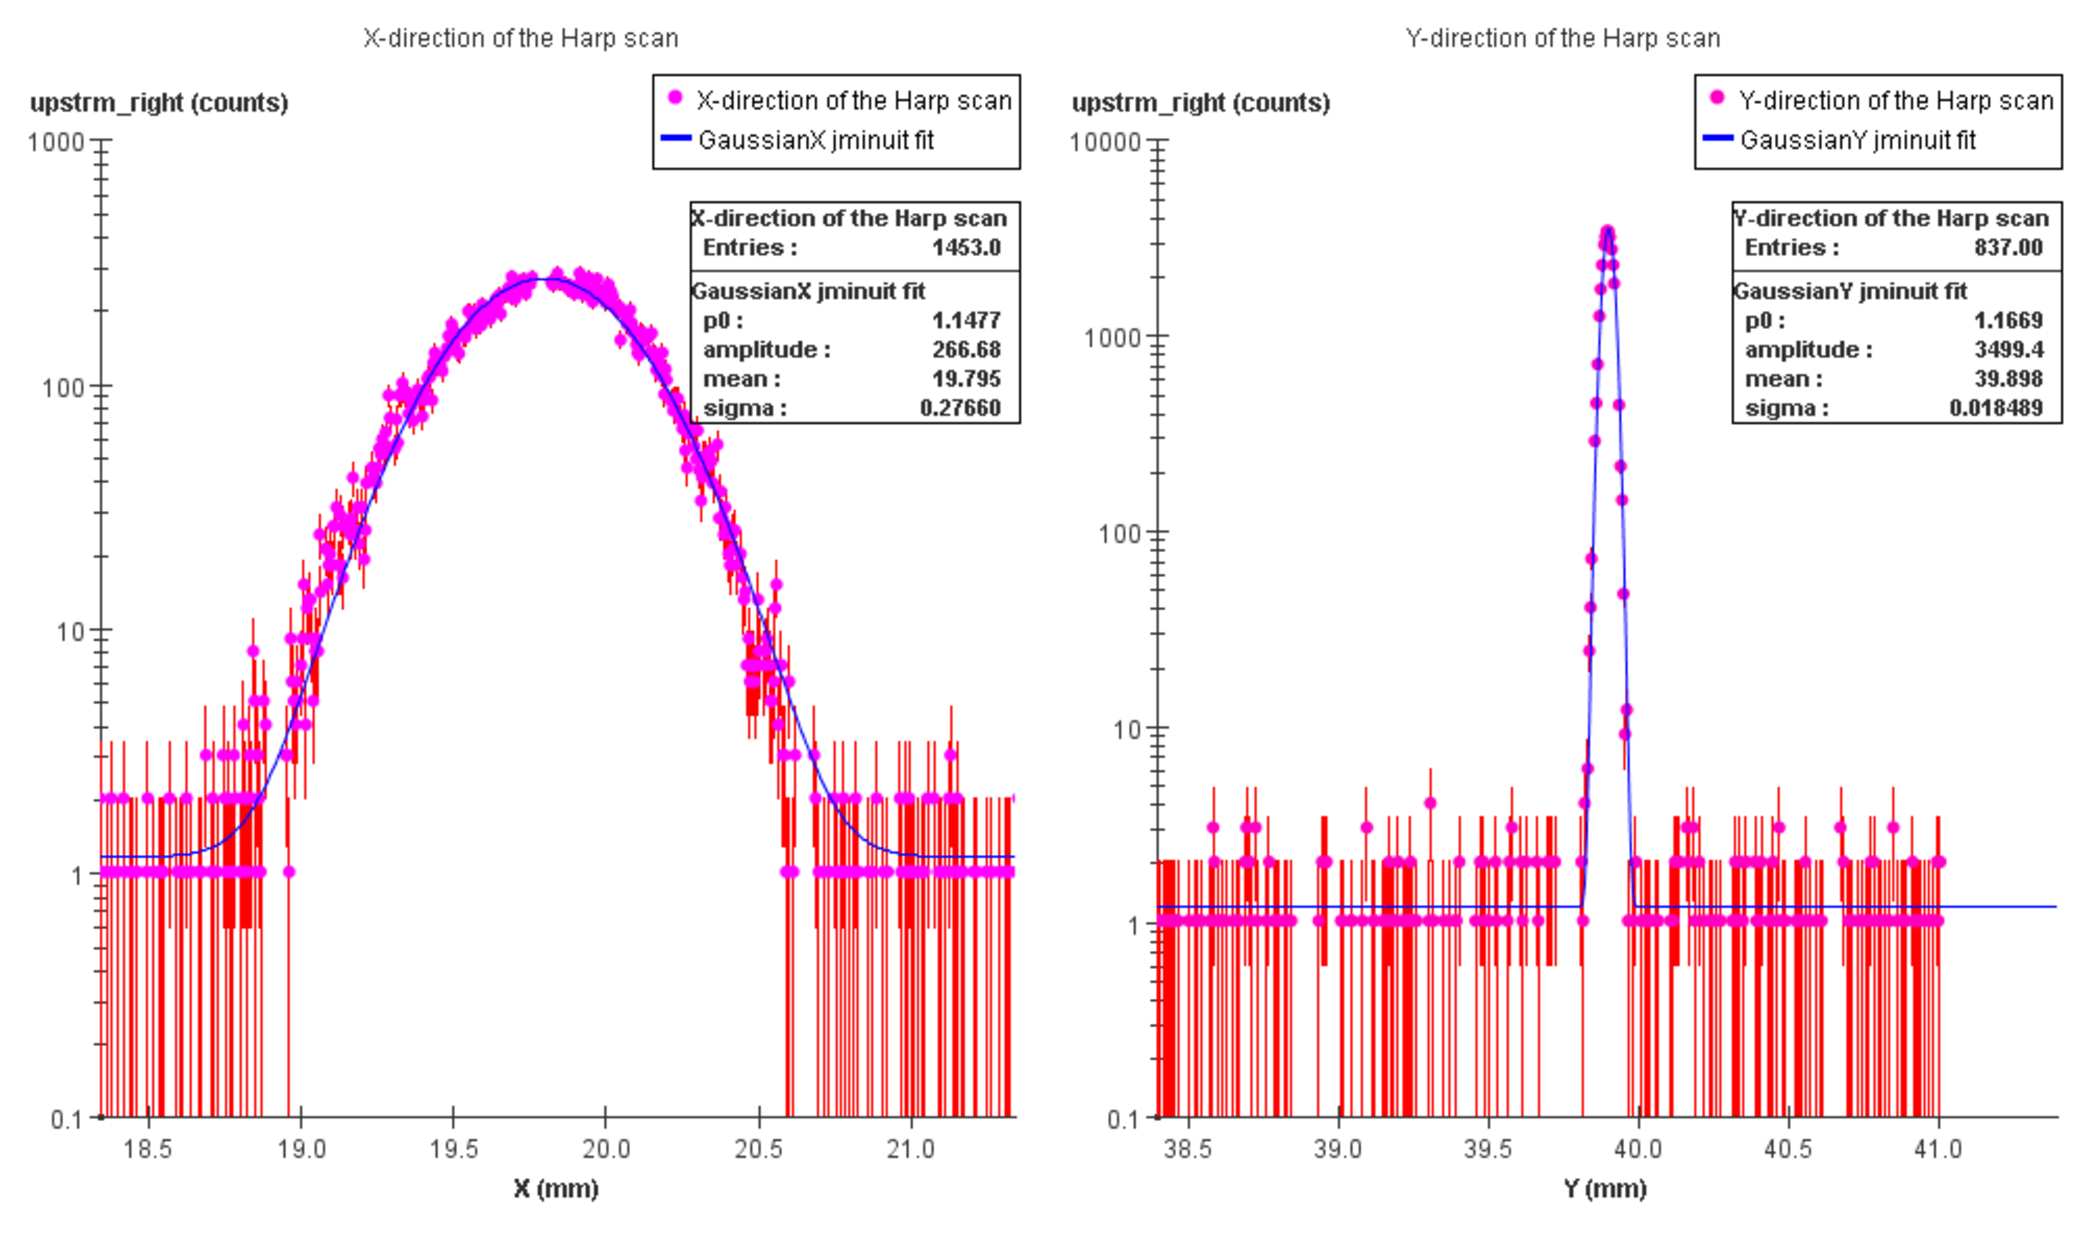
\includegraphics[scale=0.45]{beamline/harp_02.pdf}
\caption{\small{Wire harp scan after loading optics parameters from the ELEGANT program. The wire scan speed was 0.1mm/s, 
readout speed is 15Hz. Based on the width of the Y-profile, the beam position stability is  $< 20 \mu$m. Note: any beam motion with more 
than 10 $\mu$m amplitude and faster than 1Hz is included in the scan.}}\label{fig:profile_test}
\end{figure*}
 
% {\bf {\it ELEGANT for 12 GeV machine} from Arne}
The beamline optimizations have been performed for the 12 GeV CEBAF machine including the proposed changes for Hall-B/CLAS12 operations. 
Using the program ELEGANT and inputting the new locations of magnetic elements and their field maps, the beam profile was optimized at the HPS 
target location. In Figure \ref{fig:hps2014} the beam sizes and the beam angles are shown for $6.7$ GeV setup.  The required beam 
size is achievable within the operataing specifications of all the quadrupoles.  Since HPS will run at beam energies $<6.7$ GeV it is straight 
forward to scale (linearly) the magnets down to the other energies.  The beam size/angle (beam transport) remains the same 
for $1.1$, $2.2$, and $4.4$ GeV energies with the exception of the small emittance increase at $6.7$ GeV.
  
  \begin{figure*}[t]
%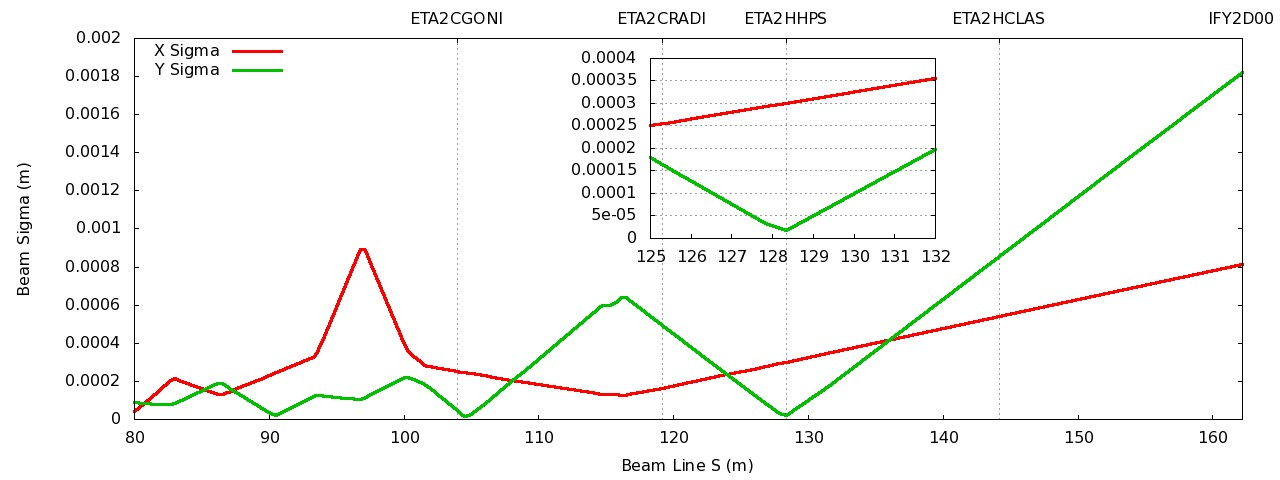
\includegraphics[scale=0.35]{beamline/hps_test_300_by_15.jpg}
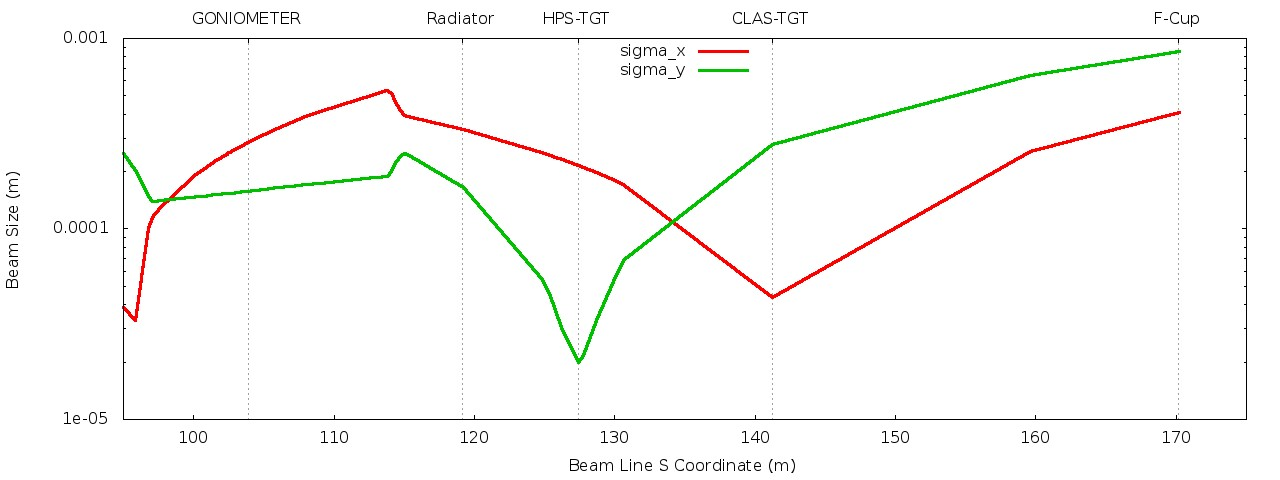
\includegraphics[scale=0.35]{beamline/hps2014_beamsize.jpg}
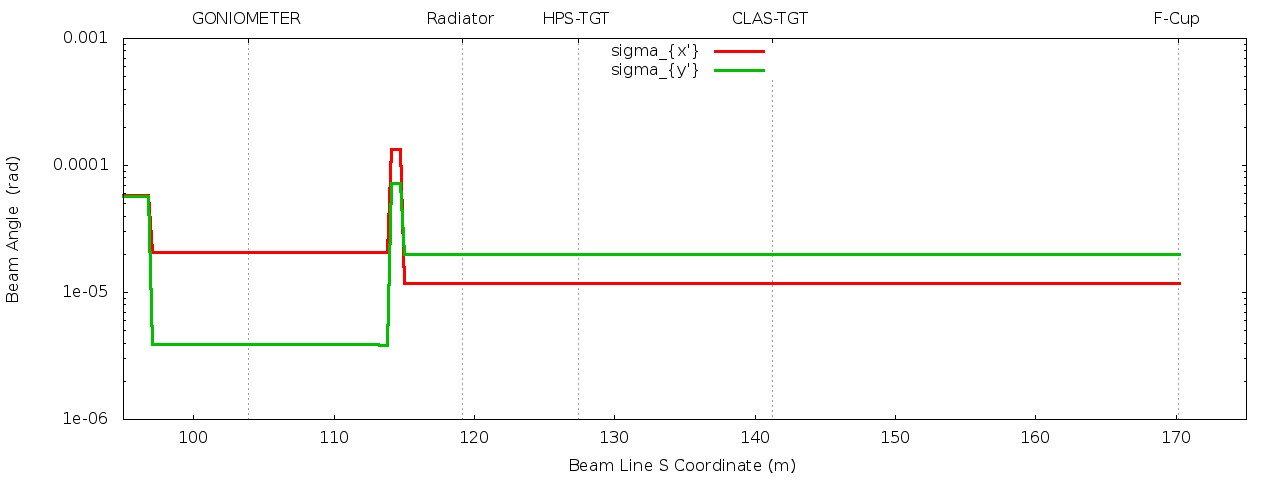
\includegraphics[scale=0.35]{beamline/hps2014_beamangle.jpg}
\caption{\small{Beam sizes in X and Y along the B-line in the upstream tunnel and in the region of the HPS test run setup. At the HPS target an 
asymmetric beam profile $\sigma_X=300 \mu$m and $\sigma_Y=20 \mu$m can be achieved with existing B-line optics.}}\label{fig:hps2014}
\end{figure*}


 
 \subsubsection{Beam Diagnostics}
 \label{setup:beam_dignostics}
 
Beam position and current will be controlled using inputs from two sets of cavity beam position monitors (BPMs), that are located in the 
upstream tunnel (see Figure \ref{fig:upstream_beamline}). 
Sets of corrector dipoles and quadrupoles are routinely used to tune the beam for Hall B (2C21 to 2C24). A pair of BPMs, 2C21 and 2C24, 
will define the incoming trajectory of the beam and are included in the fast feedback loop. Readings from these BPMs will be used to 
maintain stable beam positions and currents. The stability of beam positions at two different locations also ensures the stability of the 
beam inclination.
 
\begin{figure*}[!ht]
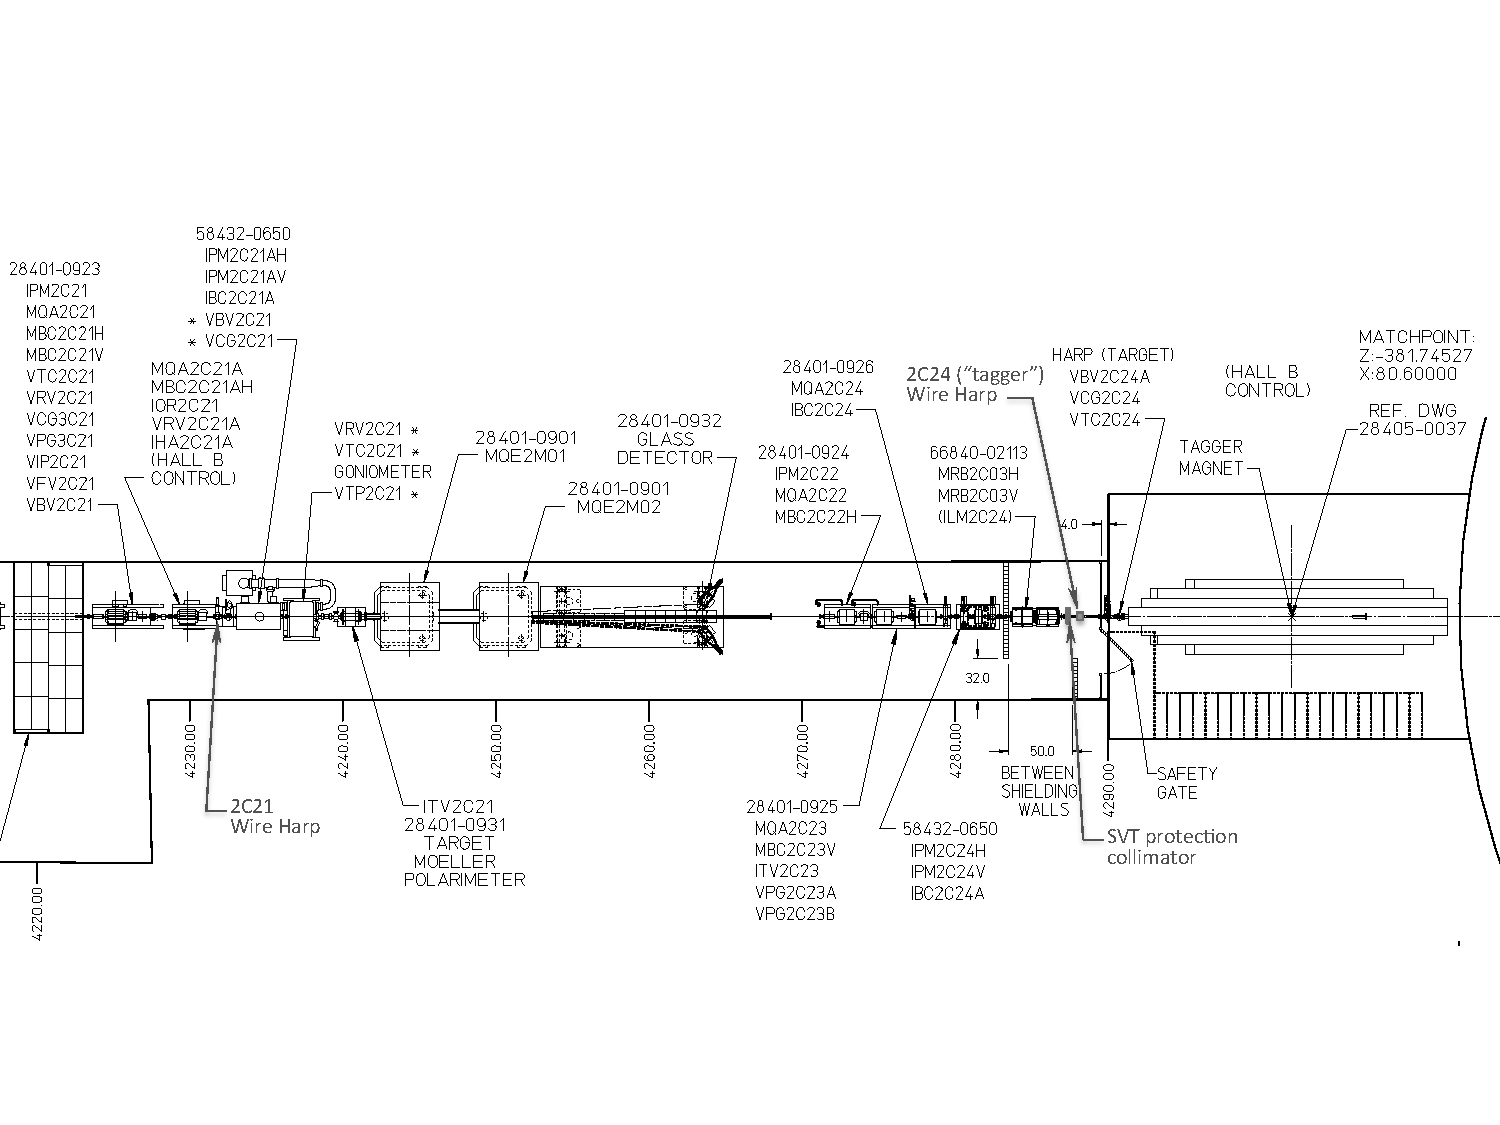
\includegraphics[angle=90, width=0.95\textwidth]{beamline/upstream_beamline}
\caption{\small{Upstream beam line configuration for HPS.}}\label{fig:upstream_beamline}
\end{figure*}

The beam profile will be measured using three wire scanners. Two are installed in the tunnel, the first one at 2C23, and the second one before the 
Hall-B tagger magnet, (2c24 harp, called ``tagger harp''), about 8 meters upstream of the HPS target. The third wire harp, 2H00 harp, will 
be located just before the first chicane dipole. The first two profilers will be used to establish the required beam parameters during the 
initial setup. The Hall-B tagger magnet will be energized when beam tune is in progress, diverting the beam away from the HPS apparatus.
After an acceptable beam profile is achieved, the tagger magnet will be degaussed and turned off, and the beam 
will be put through the HPS system and the beam profile will be checked using the 2H00 wire harp. 
The backgrounds in the HPS silicon tracker from beam profiling using the 2H00 harp have been simulated. At $5$ nA beam current, the 
radiation damage is equivalent to about $10$ sec. of production beam current on the HPS target, so is not a concern.

A set of tungsten beam-fiducial wires will be installed immediately in front of the silicon detectors in the experiment's analyzing magnet. One horizontal wire, 20 micron diameter, and one 30 micron wire at 9 degrees to the horizontal, will be mounted on a frame attached to the upper movable silicon support plate, and similarly for the bottom plate. The frames for the wires are wide enough that they do not occlude the silicon active area. The wires can be used to locate the position of the beam relative to the silicon. To accomplish this safely, the vertical separation between the front silicon sensor and its nearest wire is 8 mm. This separation, and the small wire diameters, also means that, when the sensors are positioned for data taking, the wires will have a negligible effect on acceptance. The wires are also available for use as a fairly conventional wire scanner. In particular they can provide information about the minor and major axes, and the tip angle (roll), of a strongly elliptical beam.

An insertable YAG screen beam viewer will be installed in the downstream alcove of Hall-B, before the Faraday cup, $\sim 40$ meters downstream 
of the HPS target. Both the position and profile of the beam will be used to setup the chicane magnets and to monitor beam quality during the run. 
A set of beam halo counters mounted along the beam line provides continuous and fast monitoring of the beam conditions. These counters are 
like those used for beam profile measurements. Excess noise in the beam halo counters triggers the machine fast
shutdown system (FSD) in order to terminate beam in the event of beam excursions which could damage the HPS detectors. The FSD will occur 
in less than 40 $\mu$s. In addition to halo counters, a beam offset monitor (BOM) will be installed upstream of the 2H00 wire harp. It is 
similar to the BOM used in CLAS. A short quartz cylinder, about $6$ mm OD and $4$ mm ID, with optical fibers attached around the edge will be centered 
on the beam. Even a few electrons in the beam tail will generate light in the cylinder that will be detected in a multi-anode PMT attached to 
the readout fibers. Errant beam motion towards the collimator located upstream of the tagger magnet will generate more light and increase the counts 
in the quartz cylinder, signalling a potential problem. The BOM will be wired to FSD as part of the equipment protection system. 
 
\subsubsection{Vacuum chambers} 
\label{vacchamb}
 
The SVT vacuum box will be attached to the existing magnet vacuum chamber as shown in Figure \ref{fig:svtvbox}. Power, high voltage, and data 
signals to and from the hybrids are connected through two $8$" flanges on the sides of the vacuum box. Two vertical linear motion mechanisms 
driven by stepper motors 
are used to position the SVT upper and lower modules with a precision of $1.25 ~\mu$m/step. A third linear motion mechanism is used to position 
the target on or off the beam. All the stepper motors are placed at a large enough distance from the magnet to avoid any ill effect from the 
magnetic fringe field.
An existing stepper motor driver and  EPICS-based control software will be used.   
 
\begin{figure*}[t]
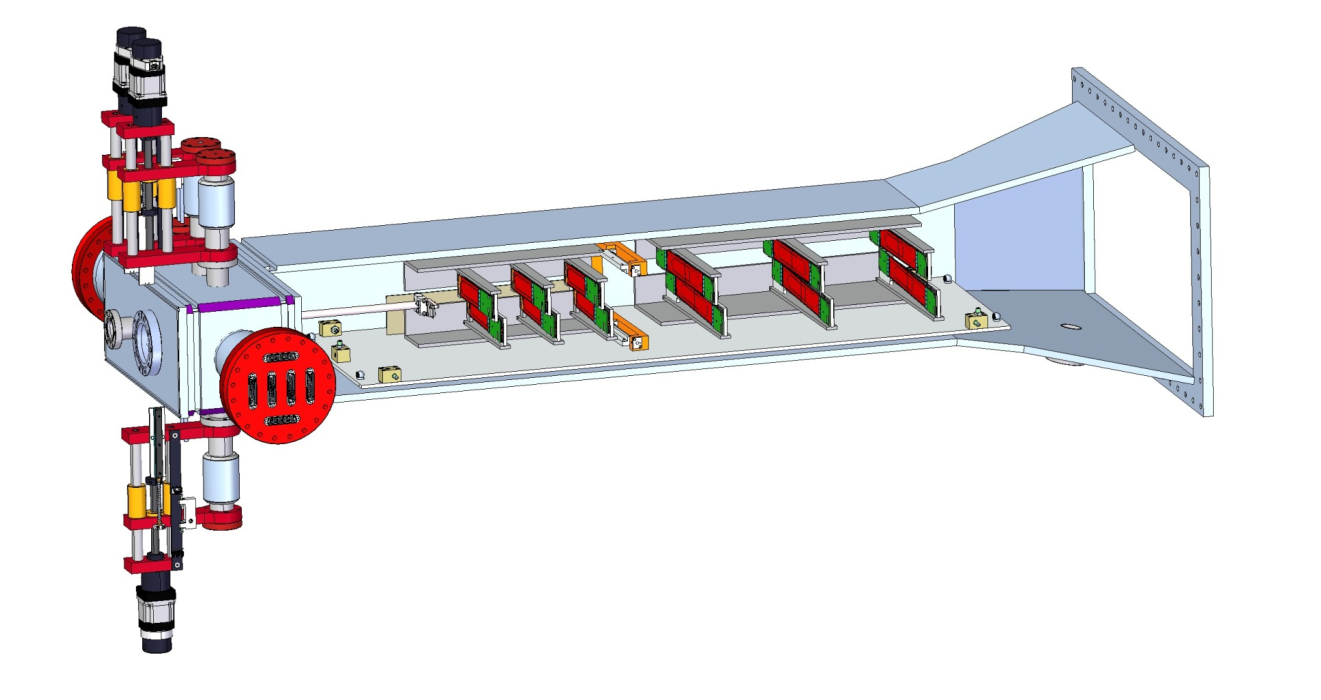
\includegraphics[scale=0.75]{beamline/svt_in.pdf}
\caption{\small{Rendering of the SVT inside the Hall-B pair spectrometer vacuum chamber and the upstream vacuum box with SVT and target connections.}}\label{fig:svtvbox}
\end{figure*}

The scattering chamber between the top and bottom parts of the ECal is a critical beamline element. In order to keep the calorimeter as close as 
possible to the beam plane, include sufficient thermal insulation for the ECal, and maintain as wide a vacuum gap as possible, the top and bottom 
plates of the scattering chamber must be quite thin. At the location where the primary beams  ($e^-$ and $\gamma$) exit, the openings in the 
chamber have been enlarged. In Figure \ref{fig:ecalv} a rendering of the scattering chamber in between the two halves of the ECAL is shown. The 
front flange of the chamber connects directly to the magnet vacuum chamber. Vacuum is maintained only on the electron side (beam right) since 
the backgrounds on the positron side are negligible.  
This design is based on detailed GEANT4 simulations of the background rates and acceptance of the ECal. It places crystals within 20 mm 
from the beam plane to maximize low-mass acceptance. In order to avoid excessive deformation of the thin walls of the vacuum chamber, an aluminum 
honeycomb support is inserted between the upper and lower walls, to beam's right.

The ECal vacuum chamber will be connected to the muon system vacuum chamber, located between the two halves of the muon system. Special openings for 
the photon and electron beams are not needed in the muon system vacuum chamber. The gaps for the radiated secondary electrons are essentially 
projections of those in the ECal vacuum chamber. At its 
upstream end, the muon vacuum chamber will have a gap of $\sim 5$ cm. At the downstream end that gap will be $\sim 7.5$ cm.

The last vacuum chamber, which passes through the third dipole, does not need to have a narrow opening. It will have size of the Frascati H magnet 
gap. At the downstream end of this chamber, there will be flange with two exit windows, a Kapton window for the photon beam to exit the chamber 
and go to 
the photon beam dump through a Helium bag, and a vacuum continuation to the standard beam line for the electron beam to go to the Hall-B 
electron beam dump. 

\begin{figure*}[t]
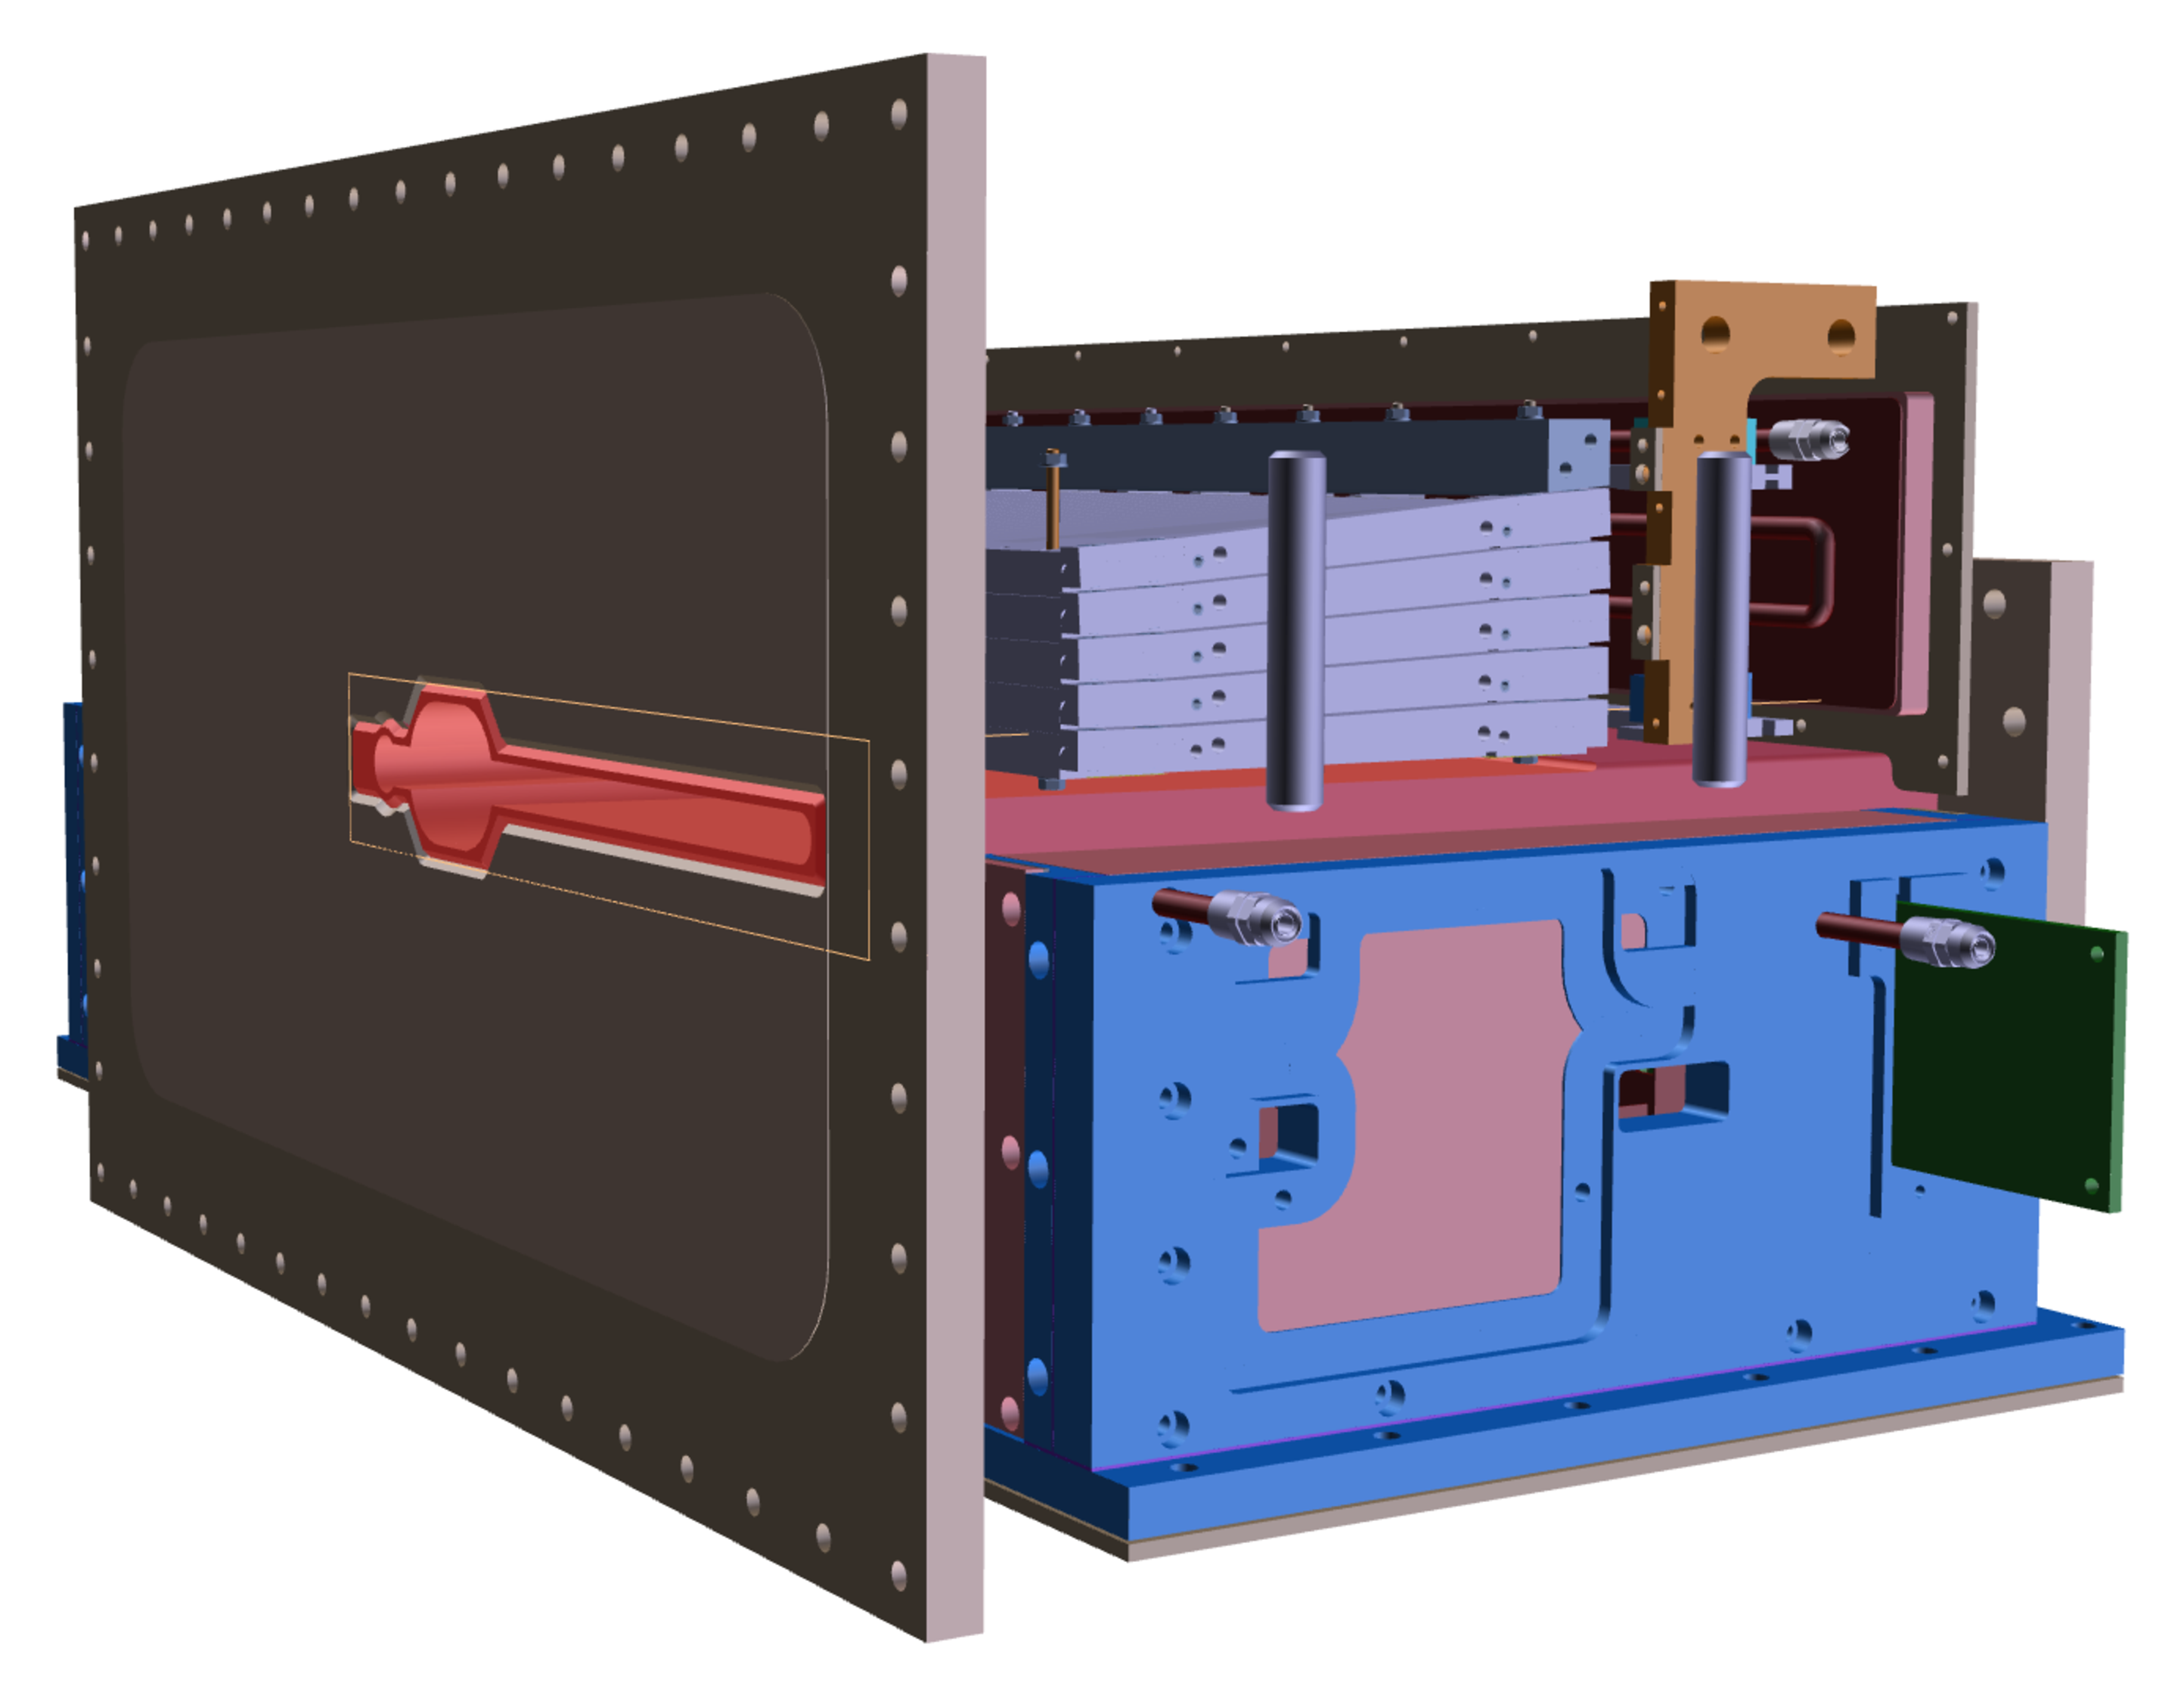
\includegraphics[scale=0.25]{beamline/ecal_vac.pdf}
\caption{\small{Rendering of the ECal and the ECal vacuum chamber.}}\label{fig:ecalv}
\end{figure*}
 
\subsubsection{Beam dumps and shieldings} 

The Hall-B electron beam dump will be used to terminate the electron beam. Due to its high intensity, the beam will not be dumped in the Faraday 
cup (FC); instead, the existing beam blocker before the FC will be used to terminate the beam. The photon beam will be dumped in a photon beam dump, 
which will be a hut  made of lead bricks located on the space frame. There will be a shielding wall after the last chicane magnet to prevent 
radiation from reaching the detector systems on the downstream side of the Hall.

\subsubsection{Targets} 
\label{target}

A thin tungsten foil is used as the target. High Z material is
chosen for its short radiation length, to minimize the hadronic
production relative to the electromagnetic trident and $A'$
production. The target is located 10 cm in front of the first
plane of silicon strip detectors.

The primary target, 10 mm square, is 0.00125 radiation lengths
(approximately 4 $\mu$m tungsten). Mounted immediately above it
is a similar area of 0.0025 radiation lengths, available for some
of the data taking, adjusting the beam current as appropriate.
The foil can be fully retracted from the beam, and is inserted on
to the beam line from above, using a stepping motor linear
actuator. The bottom edge of the foil is free-standing so there
is no thick support frame to trip the beam when the target is
inserted. Its position is adjustable vertically allowing either
thickness to be selected, and different sections of the
tungsten can be used in the event of beam damage. The support
frame on the beam-right side of the target is made thin enough to
prevent radiation damage to the silicon in the event of an errant
beam caused, for example, by an upstream chicane magnet trip.
               
The target is intended to operate with beam currents up to 500
nA, which produce strong local heating. The strength of tungsten
drops by an order of magnitude with temperature increases in the
range of 1000 C. In addition, the material re-crystallizes above
this range, which increases the tendency for cracking where
thermal expansion has caused temporary dimpling. For these
reasons, it was decided to keep the temperature rise less than
about 1000 degrees, which is accomplished by selecting an
adequately large beam spot area. For example at 200 nA the rms
beam radii will be held above 20 by 250 $\mu$m, or 40 by 250
$\mu$m for 400 nA. Simulations have shown that these beam spot
sizes do not diminish the pair reconstruction resolution of the
experiment.


 

\clearpage

\subsection{Silicon vertex tracker {\it Tim}}
\label{sec:svtŧ}


\subsubsection{Sensor Modules}

The sensor modules for the SVT consist of a pair of identical half-modules, sandwiched back-to-back around an aluminum cooling block at one end and a similar PEEK spacer block at the other. Figure \ref{fig:tracker_module} shows a prototype module assembly.
\begin{figure}[ht]
    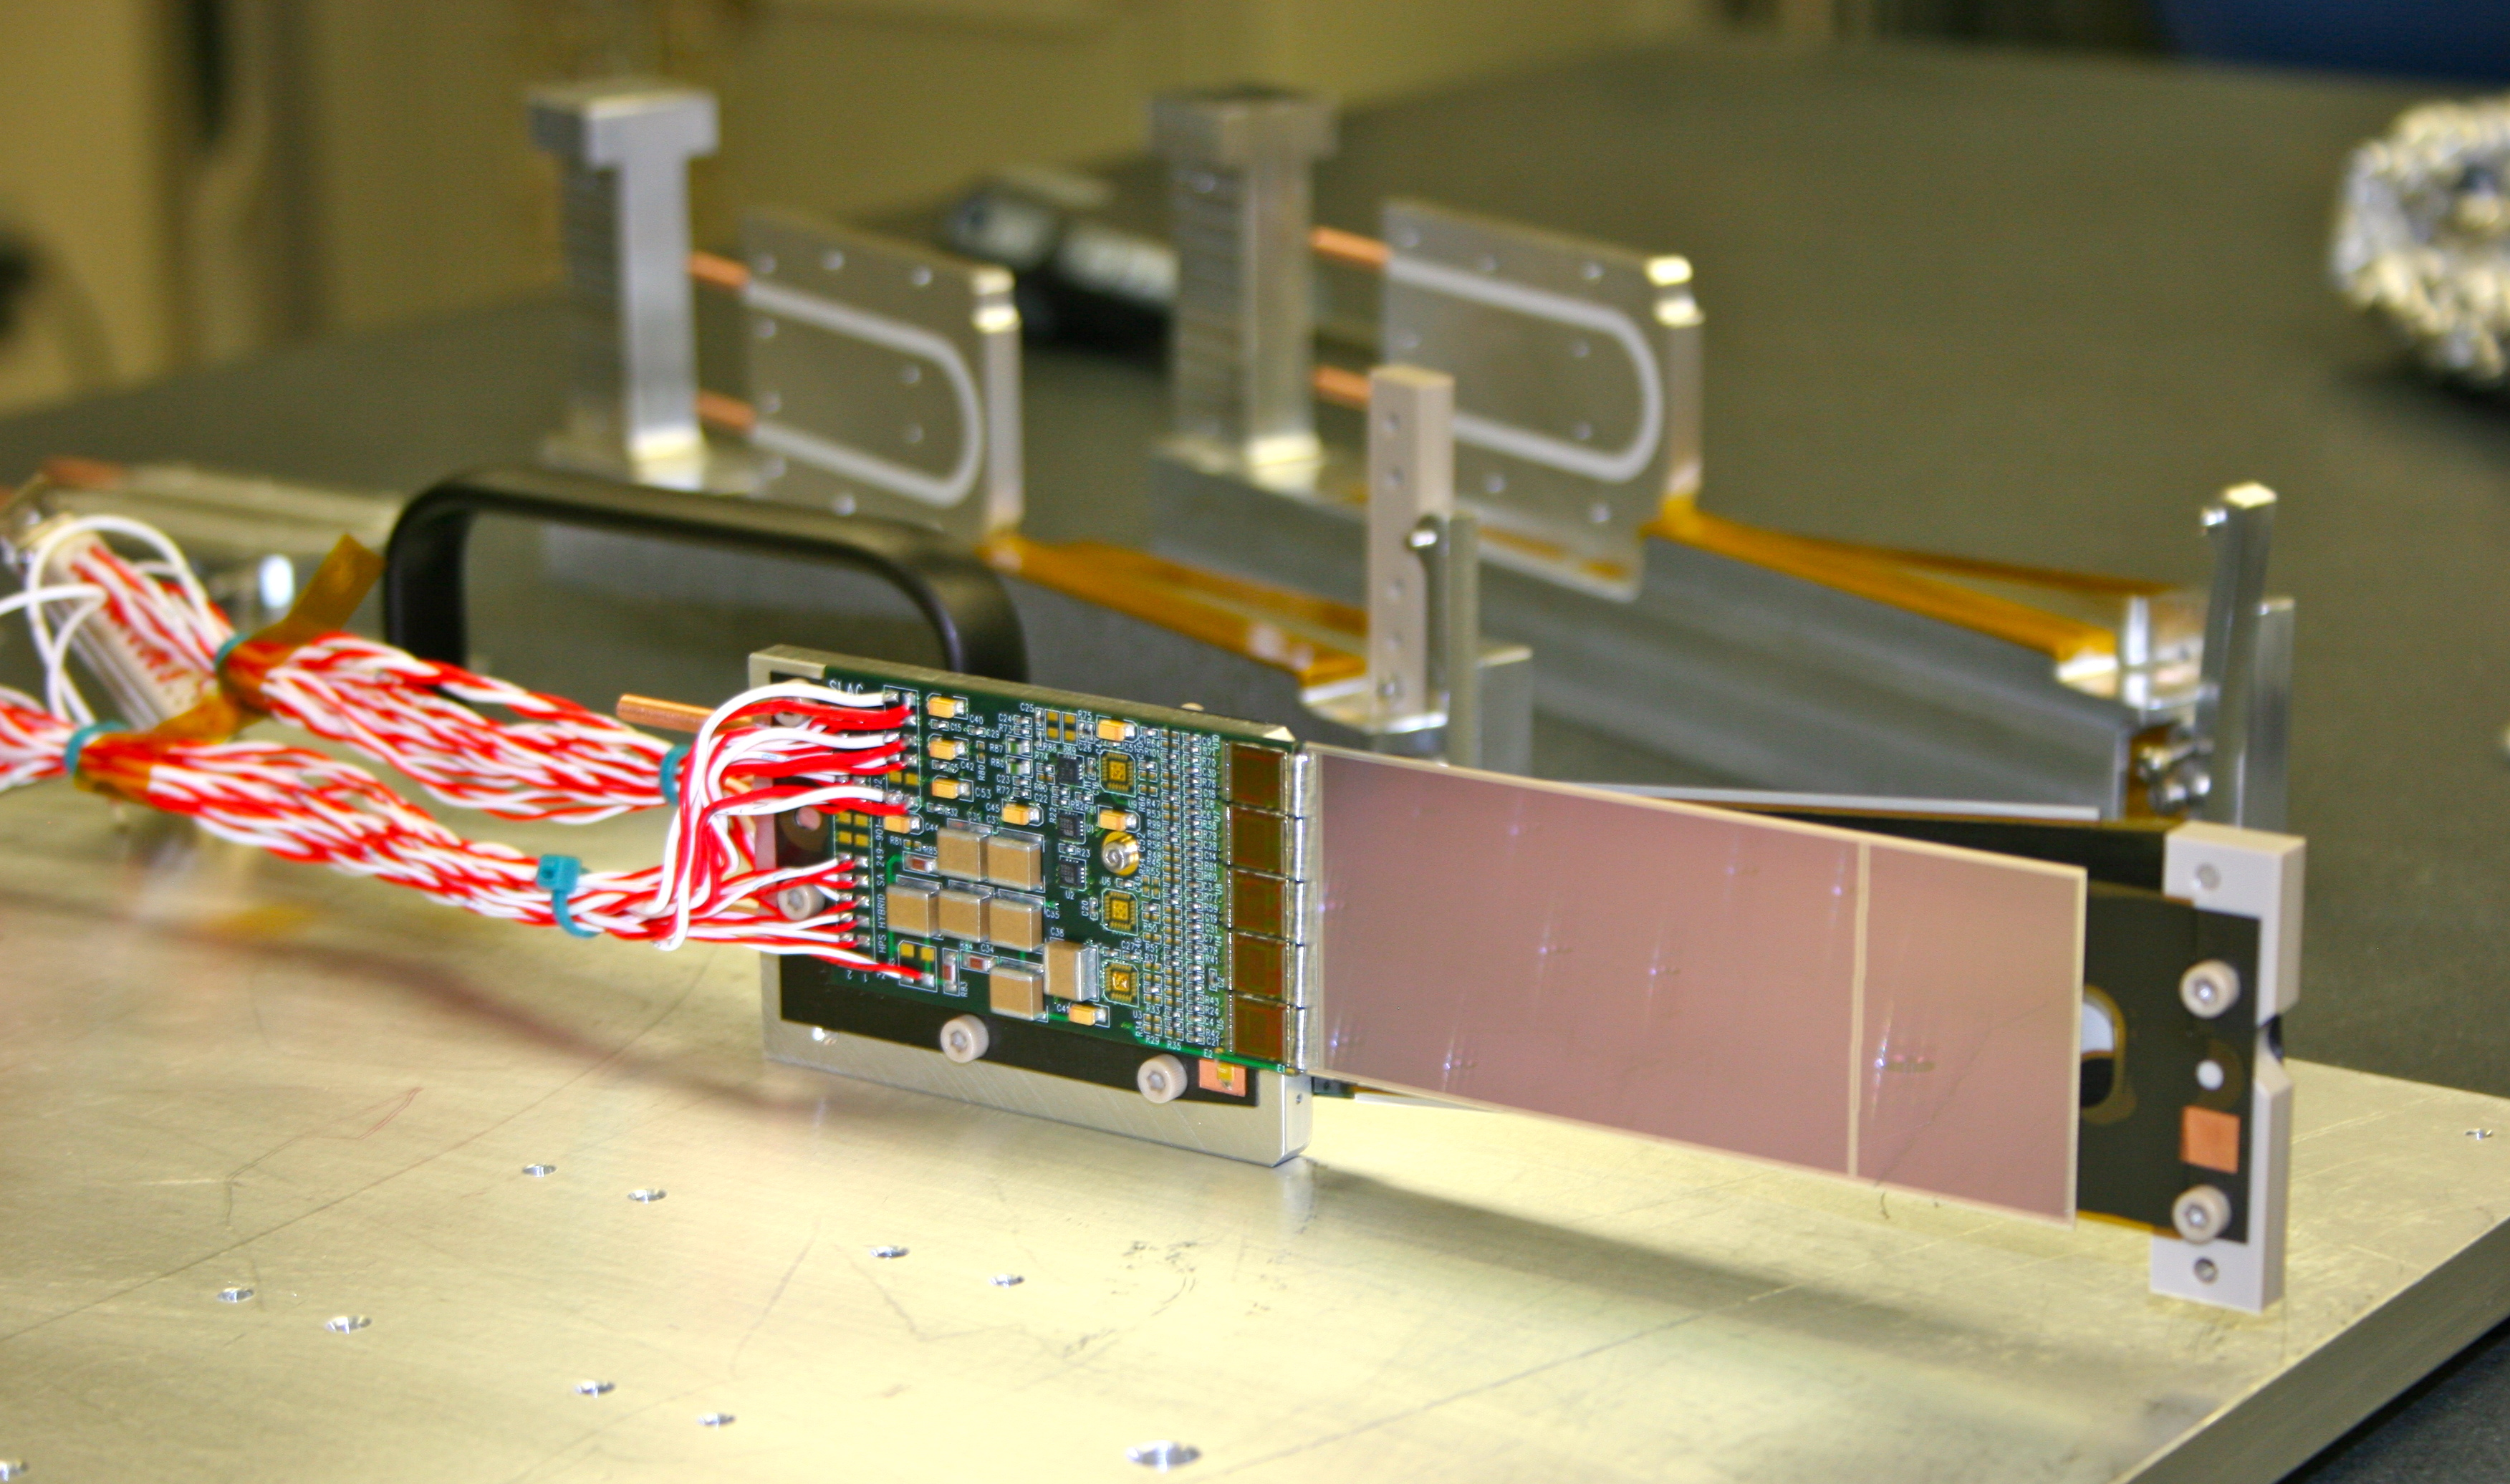
\includegraphics[width=\textwidth]{svt/IMG_5200}
\caption{\small{A prototype module assembly (foreground) with the 50 mrad (left) and 100 mrad (right) module assembly fixtures in the background.  A pair of cooling blocks and a spacer block can be seen on the fixtures.} }
\label{fig:tracker_module}
\end{figure}
The cooling block provides the primary mechanical support for the module as well as cooling via copper tubes pressed into grooves in the plates. The spacer block defines the spacing between the sensors at the far end of the module, stiffens the module structure, and improves the stability of the sensor alignments.  

Each half module consists of a single sensor and a hybrid electronic readout board glued to a polyamide-laminated carbon fiber composite backing.  A window is machined in the carbon fiber leaving only a frame around the periphery of the silicon to minimize material. A 50 $\mu$m sheet of polyamide is laminated to the surface of the carbon fiber with 1 mm overhang at all openings to ensure good isolation between the backside of the sensor, carrying high-voltage bias, and the carbon fiber which is held near ground.  The average support material in the tracking volume is approximately 0.1\% $X_{0}$ per double-sided module.

The sensors are 320 $\mu$m thick, p$^+$ on n-bulk, $<$100$>$, single-sided microstrip sensors manufactured by the Hamamatsu Photonics Corporation for production of layers 2-5 of the D$\O$ Run IIb silicon tracker. Of 33 sensors provided for the SVT, 29 had breakdown voltages in excess of 1000V and all but 4 had no bad channels.  

The readout ASICs are the APV25 readout chip designed for the CMS experiment at the LHC.  In addition to fast readout capability and high radiation tolerance, the APV25 is capable of delivering multiple samples of the amplifier output at a specified pipeline latency which allows asynchronous use of the chip as well as the ability to reconstruct hit time to 2 ns at our high signal-to-noise ratios \cite{HPS_PROP}. Each 10-layer, polyamide hybrid readout board hosts a set of five APV25 and provides conditioned high-voltage for biasing the sensor. Power, control and data for the hybrids are connected via 30 lines of twisted pair wire: an 18~cm ``pigtail'' cable is soldered directly to the surface of the hybrid.  Bias is provided to both top and back side via wire bonds which are also used to connect the front end reference to the carbon fiber. All wire bonds are encapsulated to prevent damage.

Module yields were good for such a small production.  Of 165 chips acquired, 150 were used to assemble 30 production hybrids, of which 29 passed QA testing.  Of 29 modules built, 28 passed QA testing, leaving 8 spare modules after completion of the HPS Test SVT.

\clearpage

\subsection{Electromagnetic Calorimeter} 
\label{sec:ecal}

The Ecal, depicted in Fig. \ref{fig:ecal}, consists of $442$ lead-tungstate PbWO$_4$ crystals with avalanche photodiode (APD) readout and amplifiers. Those have all similarly short pulse widths, so that they can run at very high rates. Indeed, the expected high radiation and high rate environment, together with a high magnetic field in close proximity, essentially imposed lead-tungstate (PbWO$_4$) crystals with APD readout. The lead tungsten (PbWO$_4$) crystals are taken from the Inner Calorimeter (IC) of the JLab CLAS detector, which was originally build in IPN Orsay and run for 10 years with success. Crystals in the ECal are arranged in two modules. There are 5 layers in each module; four layers have $46$ crystals and one has $37$. The ECal is mounted downstream of the analyzing dipole magnet at the distance of about $137$ cm from the upstream edge of the magnet. The two ECal modules are positioned just above and below the ECal vacuum chamber, through which the beam and the wall of flame passes in vacuum. At its closest point, the edge of the crystal is at $3.7$ cm from the beam. In order to maintain stable performance of the PbWO$_4$ calorimeter, the crystals and APDs are enclosed within a temperature stabilized environment, held constant at the level of 1\!\char23F. The expected energy resolution of the system from operational experience with the IC is $\sigma_E/E \sim 4.5\%/\sqrt{E}$ (GeV). As in the IC, PbWO$_4$ modules are connected to a motherboard that provides power and transmits signals from individual APDs and pre-amplifier boards. The ECal data is digitized using the JLAB FADC250, a 250 MHz flash ADC developed for the 12 GeV Upgrade. The full analogue information from the FADCs coupled with the spatial and time information of each module are available to the trigger system, which uses energy deposition, position, timing, and energy-position correlation to reduce the trigger rate to a manageable $\sim 30$ kHz (see section \ref{seq:ECalTrigger} for details).

\begin{figure*}[t]
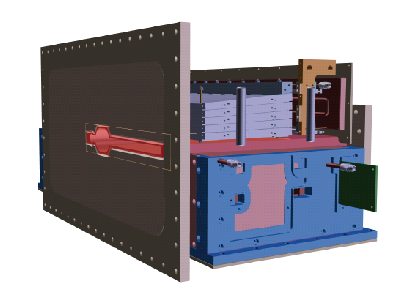
\includegraphics[scale=0.7]{ecal/ECal.png}
\caption{\small{Cut-away view of the Ecal, showing the vacuum flange which mates to the magnet vacuum chamber on the left, holes for the electron beam and the “wall of flame” in the Ecal vacuum chamber (in red), crystal positions in the upper module, and the temperature control box in blue in the lower module.}}\label{fig:ecal}
\end{figure*}

For an experiment like HPS, where backgrounds must be well understood and need to be strongly suppressed, the trigger bias can be an important issue. In particular, having a stable and known thresholds at the trigger readout are necessary in order to avoid the bias in the event selection. The uniformity of trigger response and the stability can be achieved with the installation of an online gain monitoring system. This system will introduce short light pulses in the front of the crystals. Optical fibers will be used to transmit light from the source to the crystals to test the response of APDs. The response of the system will therefore be sensitive to both transparency losses of crystals due to a possible radiation damage and gain variations of APDs. Such a system has been developed for several experiments (CMS at CERN for instance) with various light sources. The system for ECal will be developed in IPN Orsay during 2013 and in the first half of 2014, to be ready for installation at JLAB for the commissioning run at the end of 2014. We choose, for their low cost, to use two different mono-color LEDs as light sources to monitor responses of each module. A blue light, which corresponds to the domain of the crystal emission, and is very sensitive to the presence of color centers, produced by radiation damage. This light source is very useful to test variations of the response in the main domain of the emission. Impurities can anneal at room temperature and such monitoring can be sensitive to increasing of output as well, when the radiation exposure is reduced for a long period of time. A red colored light, less sensitive to the color centers, permits monitoring the APD gains more directly and thereby separates effects of APD and electronics from the crystal transparency, and provide clear information on the state of the electronics. The main challenge for the system is to guarantee stability at a level better than a couple percent to be able to identify and to adapt to the transparency variations. The test of the system will be carried-on at IPN Orsay, in order to guarantee its efficiency and also to test radiation resistance of the various materials.

The second major improvement to be done for the calorimeter consists in the implementation of new APDs, by replacing old $5\times 5$ mm$^2$ APDs with $10\times 10$ mm$^2$, Hamamatsu S8664-1010. The renewal of the APDs will resolve two issues with present modules of HPS calorimeter. First, new APDs from Hamamatsu have much better performance than the ones which are now installed on lead-tungstate crystals. Data from Hamamatsu shows that APDs made from the same wafer have excellent uniformity. With $\pm 10\%$ known uniformity at the gain of $100$, variations in bias voltage are $\sim 4.5$ V. Moreover, data provided for samples of 1300 the bias voltage difference is ~50 V, when for APDs now we have ($442$ pieces) the voltage difference is more than $100$ V. So, it is clear that with new APDs much better uniformity in the response of the calorimeter modules in the trigger can be achieved. Second, $4$ times larger readout area will ensure $4$ times more light collection and therefore $4$ time larger signal from APDs. This will allow the use of different amplifier modules with lower gain that in turn will decrease electronic noise. Tests performed for another calorimeter, now in production at INFN Genova for JLAB Hall-B, showed that the same type of amplifier boards with factor 2 lower gains have noise level on the order of $<5$ MeV. Minimum ionizing energy deposition in PbWO$_4$ crystals of HPS calorimeter from cosmic muons passing through perpendicular to the crystal axis is of $\sim 15$ MeV. If energy thresholds can be moved close to $5$ MeV, then MIP peak will be seen and calorimeter can be calibrated and monitored with cosmic muons. The INFN group made the first tests with HPS crystals using Hamamtsu $10\times 10$ mm$^2$ APDs and the new amplifier boards. In Figure \ref{fig:mip10x10} charge distribution of the single crystal system is shown. The red line histogram is for all events triggered by scintillation telescope located above and below the crystal. The black line histogram corresponds to charge distribution within $100$ ns of coincidence time. The MIP peak is clearly visible and well isolated from the pedestal (noise). The same crystal with old $5\times 5$ mm$^2$ APD also gets the signal from MIP, but the MIP charge distribution is under the noise peak and does not have well defined peak position, see Figure \ref{fig:mip5x5}. Possibility of detecting MIP particles traversing the system in perpendicular direction will allow to calibrate the modules with cosmic muons while they are installed in the detector. This is a great advantage and together with light monitoring system will ensure stable and reliable performance of the ECal and the trigger system. In addition to the possibility of calibrating the modules with cosmic muons (MIP calibration), the lower noise will allow to lower the acquisition thresholds and improve the energy resolution. The new amplifier boards have to be designed to work with new APDs. IPN Orsay will design the new boards in collaboration with JLAB. 

\begin{figure*}[t]
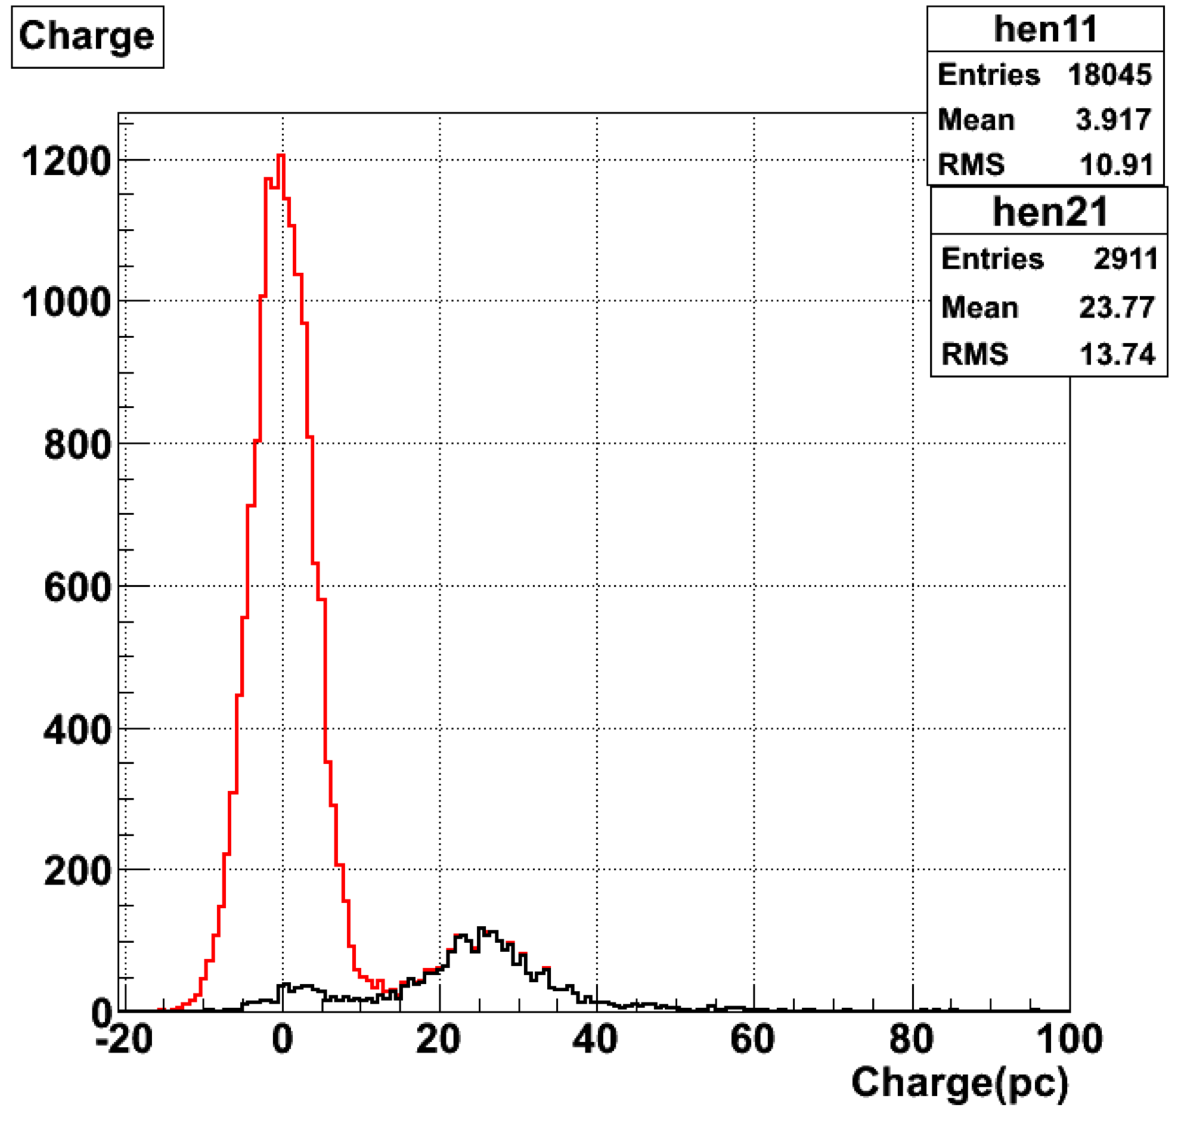
\includegraphics[scale=0.5]{ecal/MIP_10x10_APD.png}
\caption{\small{Charge distribution on QDC from readout of the HPS calorimeter crystal with Hamamatsu S8664-1010 APD and the new low noise amplifier board. The red line histogram corresponds to all events, while the black line distribution is for events within $100$ ns of the trigger signal from the scintillation telescope.}}\label{fig:mip10x10}
\end{figure*}

\begin{figure*}[t]
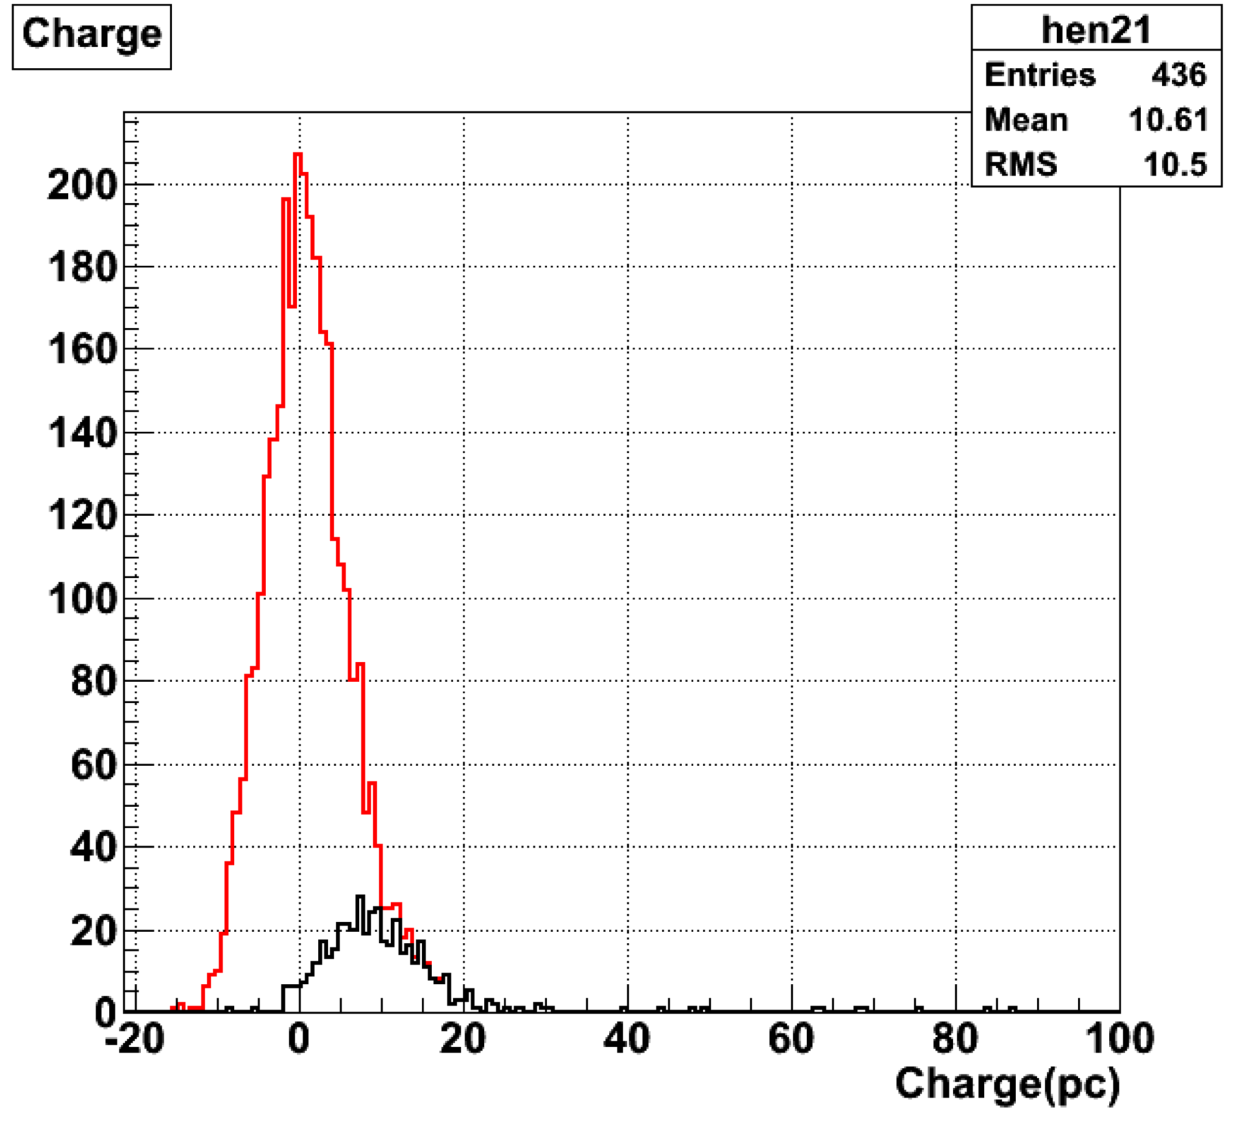
\includegraphics[scale=0.5]{ecal/MIP_5x5_APD.png}
\caption{\small{The same as in Figure \ref{fig:mip10x10} but for readout with currently used $5\times 5$ mm$^2$ APD.}}\label{fig:mip5x5}
\end{figure*}

\clearpage

\subsection{Muon system {\it Keith, Yuri, Stepan, Larry}}

\label{sec:muon}


Searching for the A$^\prime$ in its di-muon decay mode has the advantage of having greatly reduced electromagnetic backgrounds for triggering.  The only physics background will arise from photoproduction of $\pi^+$ and $\pi^-$ pairs in the target, which aren�t fully absorbed in the ECal or absorber. The muon detector will be about 1 meter long and will consist of layers of scintillator hodoscopes sandwiched between iron absorbers. The number of layers and the thickness of absorbers is defined by the $\pi/\mu$ rejection factor. Detector was optimized using the GEANT-3 model of ECal, continued with layers of iron and scintillators. Muons in the momentum range from $1$ GeV to $4$ GeV has been studied, see \cite{HPS_PROP} for details.

In Figure \ref{fig:pmrej}, the rejection factor for charged pions is presented. As can be seen from the figure, for particles from $1$ GeV to $4$ GeV, the optimal thickness of the iron absorber for pion rejection is $\sim 75$ cm (after ECal, a $16$ cm of lead-tungstate). In the efficiency calculation for low energy particles ($< 1.7$ GeV) detection in in all four layers of scintillator hodoscopes were not considered. Depending on the momentum, particles were not traced behind the third, fourth or fifth absorber.  

\begin{figure*}[!ht]
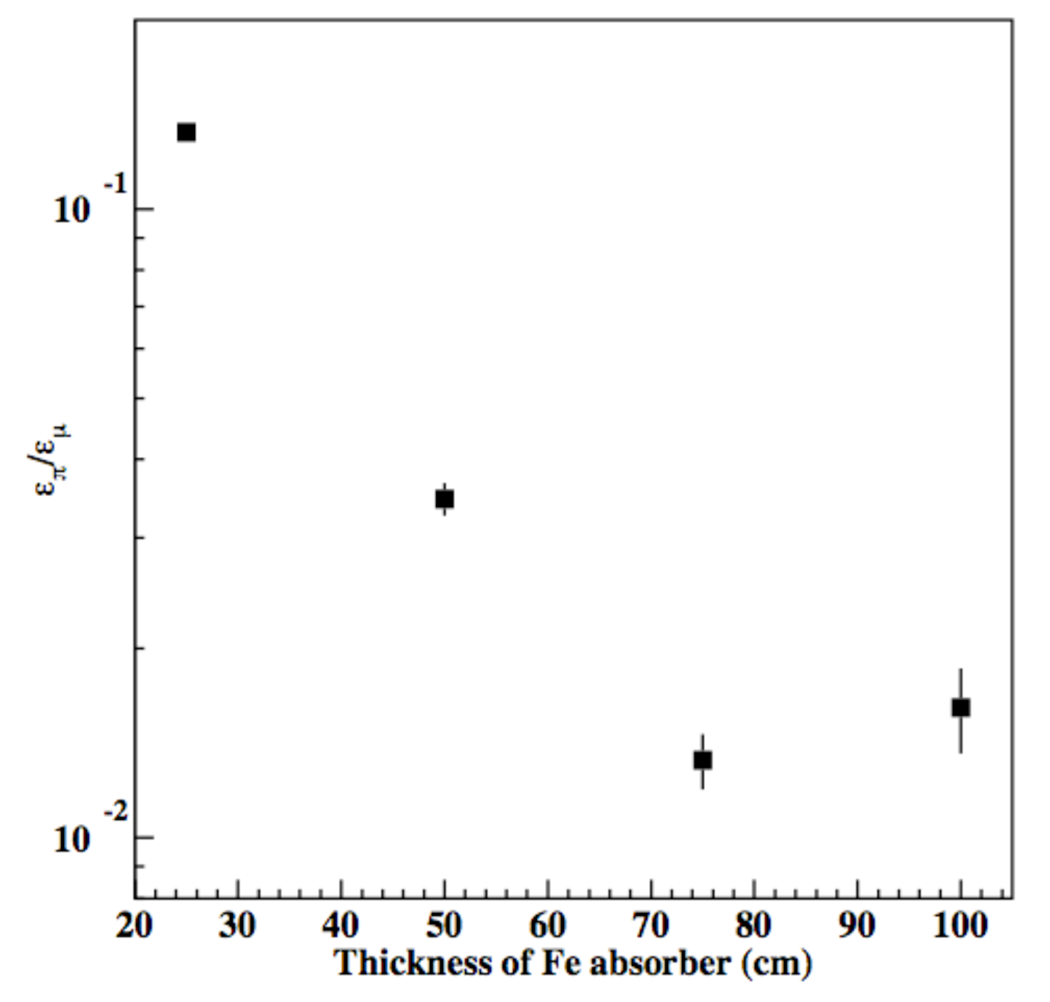
\includegraphics[scale=0.8]{muon/pmrej.pdf}
\caption{\small{Pion-muon rejection factor as a function of the iron absorber thickness.}}\label{fig:pmrej}
\end{figure*}


\subsubsection{Detector concept}

Based on simulations, a muon detector composed of a four iron absorbers (total length of $30+15+15+15=75$ cm) and four double-layer scintillator planes, positioned after each absorber layer is proposed. The muon detector will be mounted behind the ECal, see Figure 4.5.2.1. The pion rejection ($\pi/\mu$) of the proposed system as a function of particle momentum is shown in Figure \ref{fig:pmrejp}. For the determination of particle detection efficiencies, only signals in the first three layers of the hodoscope were used for momenta $< 1.7$ GeV/c. In the full momentum range from $1$ to $4$ GeV/c, $\pi/\mu$ varies from $10^{-2}$ to $2\times 10^{-2}$ and therefore the pion pair suppression factor of the system will be $< 4\times10^{-4}$. Similar to the Ecal, the muon detector will consist of two halves, one above and one below the beam. The vertical gap between the first hodoscope layers of the two halves is about 3 cm. The cross section of each half of the first hodoscope is $63\times 39$ cm$^2$. Each half of the last hodoscope layer is $74\times 46$ cm$^2$.  

\begin{figure*}[!ht]
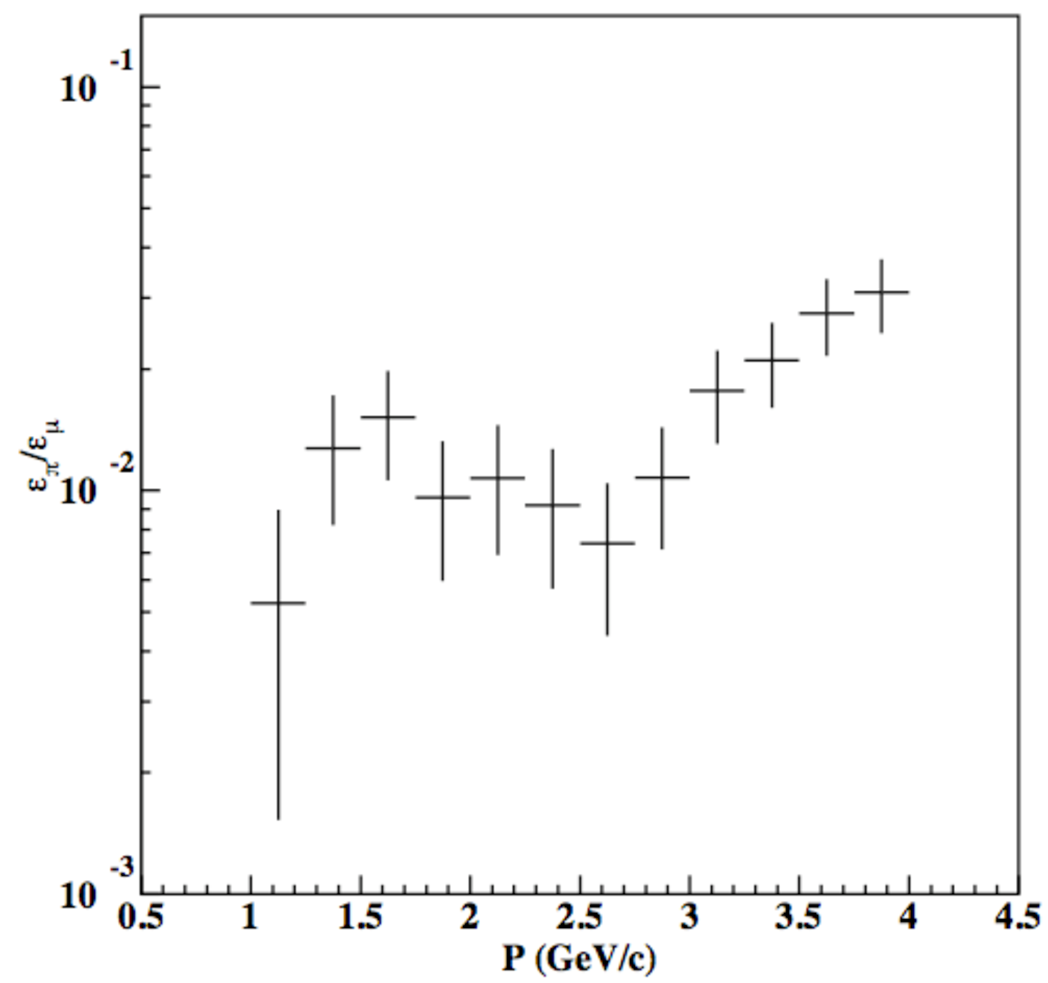
\includegraphics[scale=0.8]{muon/pmrej4.pdf}
\caption{\small{Pion-muon rejection factor as a function of the iron absorber thickness.}}\label{fig:pmrejp}
\end{figure*}

The simplest, most economical solution for the hodoscopes is to use layers of extruded scintillator strips with embedded wave-shifting fiber readout. The scintillator strips will be oriented horizontally. The light will be detected from both ends of the strip using multi-anode photomultipliers. With 5 cm vertical segmentation, a total of 144 readout channels are needed (9x16 channels multi-anode PMTs).  Signals from each channel will be sent to a TDC and to a FADC. The FADC information will be used to construct the muon trigger. The TDC information together with information from FADC will be used in offline analysis to measure the hit position along the strip. 

\clearpage

\subsection{Trigger and DAQ }
The HPS experiment data acquisition and trigger system handles the acquisition of data and 
distribution of triggers for three sub-detectors; the SVT, ECal and the muon detector. There 
are two front end electronic systems; the SVT is readout with 128-channel integrated circuits
 supported by Advanced Telecom Communications Architecture~\cite{atca} (ATCA) hardware
 while the ECal and muon detectors signals are processed by VXS based hardware. The 
 the Level 1 trigger receives input from the ECal and muon detectors only to form a decision 
 on which events to be read out.  The triggered events are acquired from the three subsystems and are processed in the data acquisition system outlined in 
 Fig.~\ref{fig:daq_hardware_overview}.
\begin{figure*}[t]
%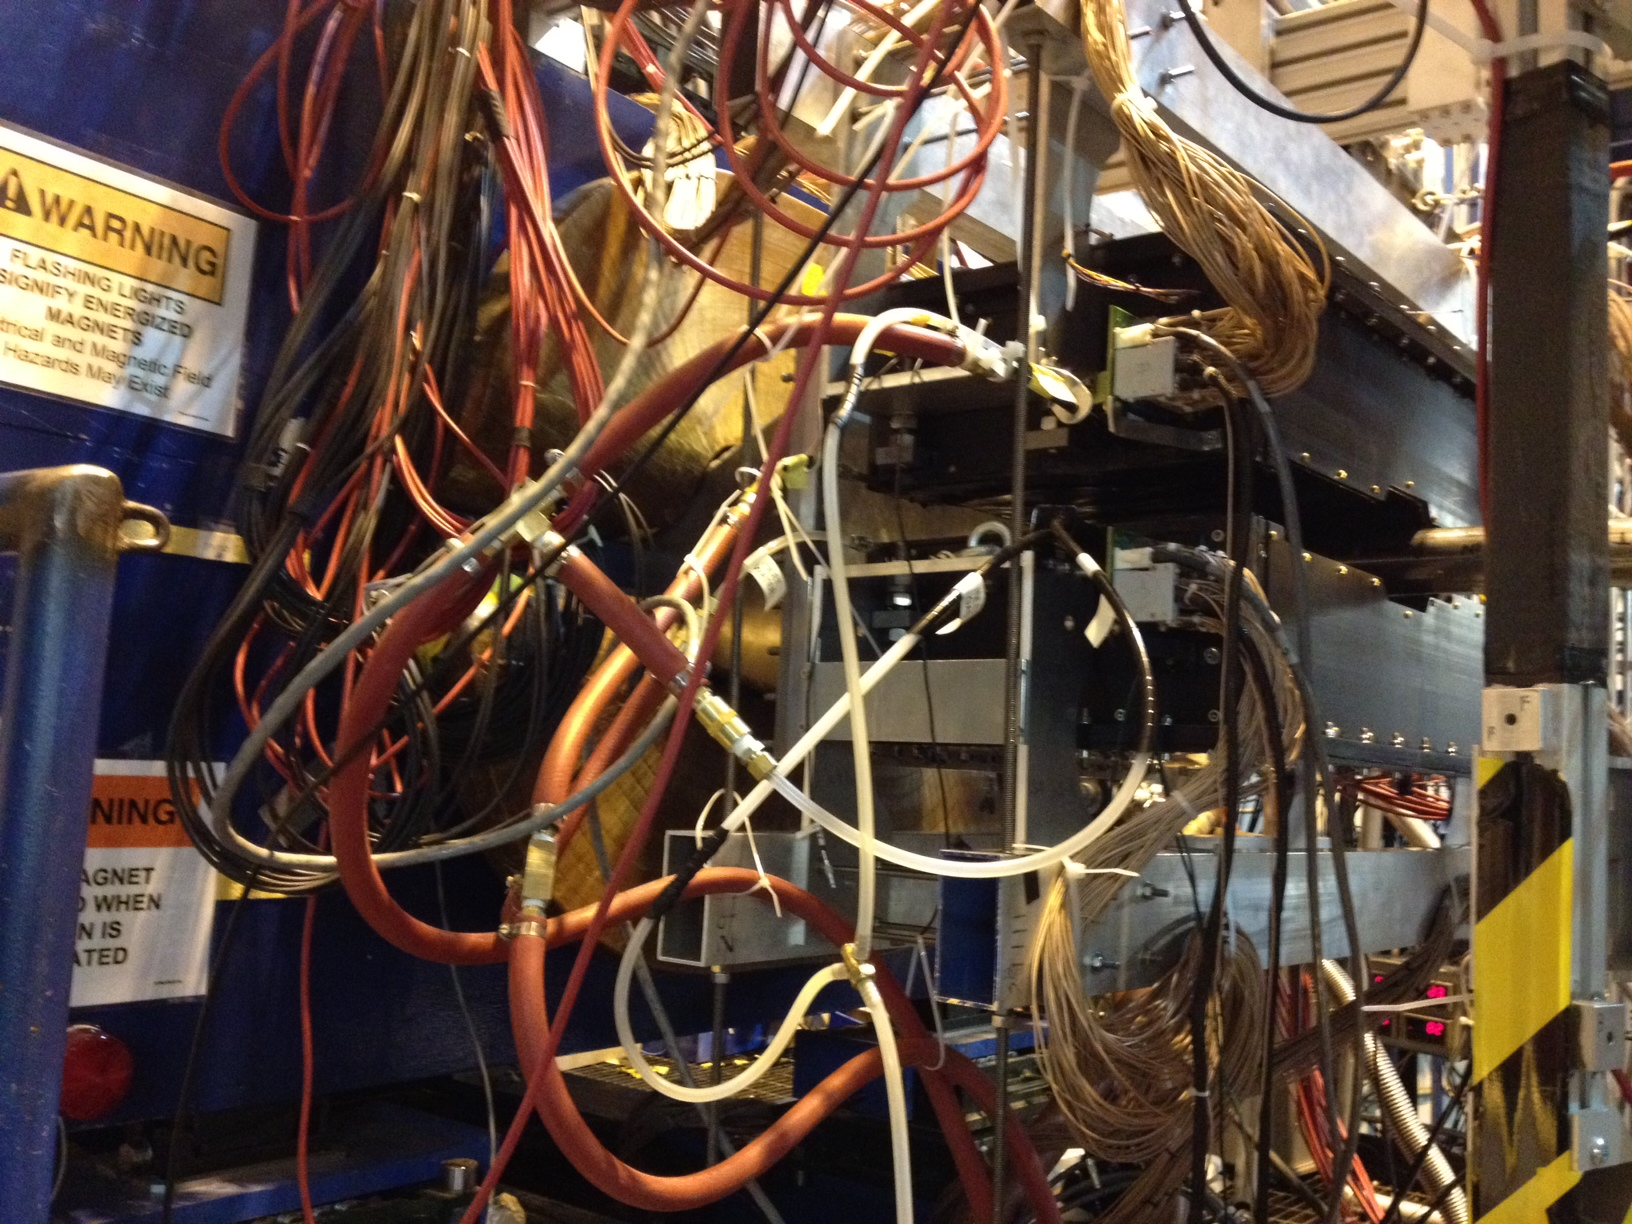
\includegraphics[ scale=0.25]{test2012/ecal_mounted.JPG}
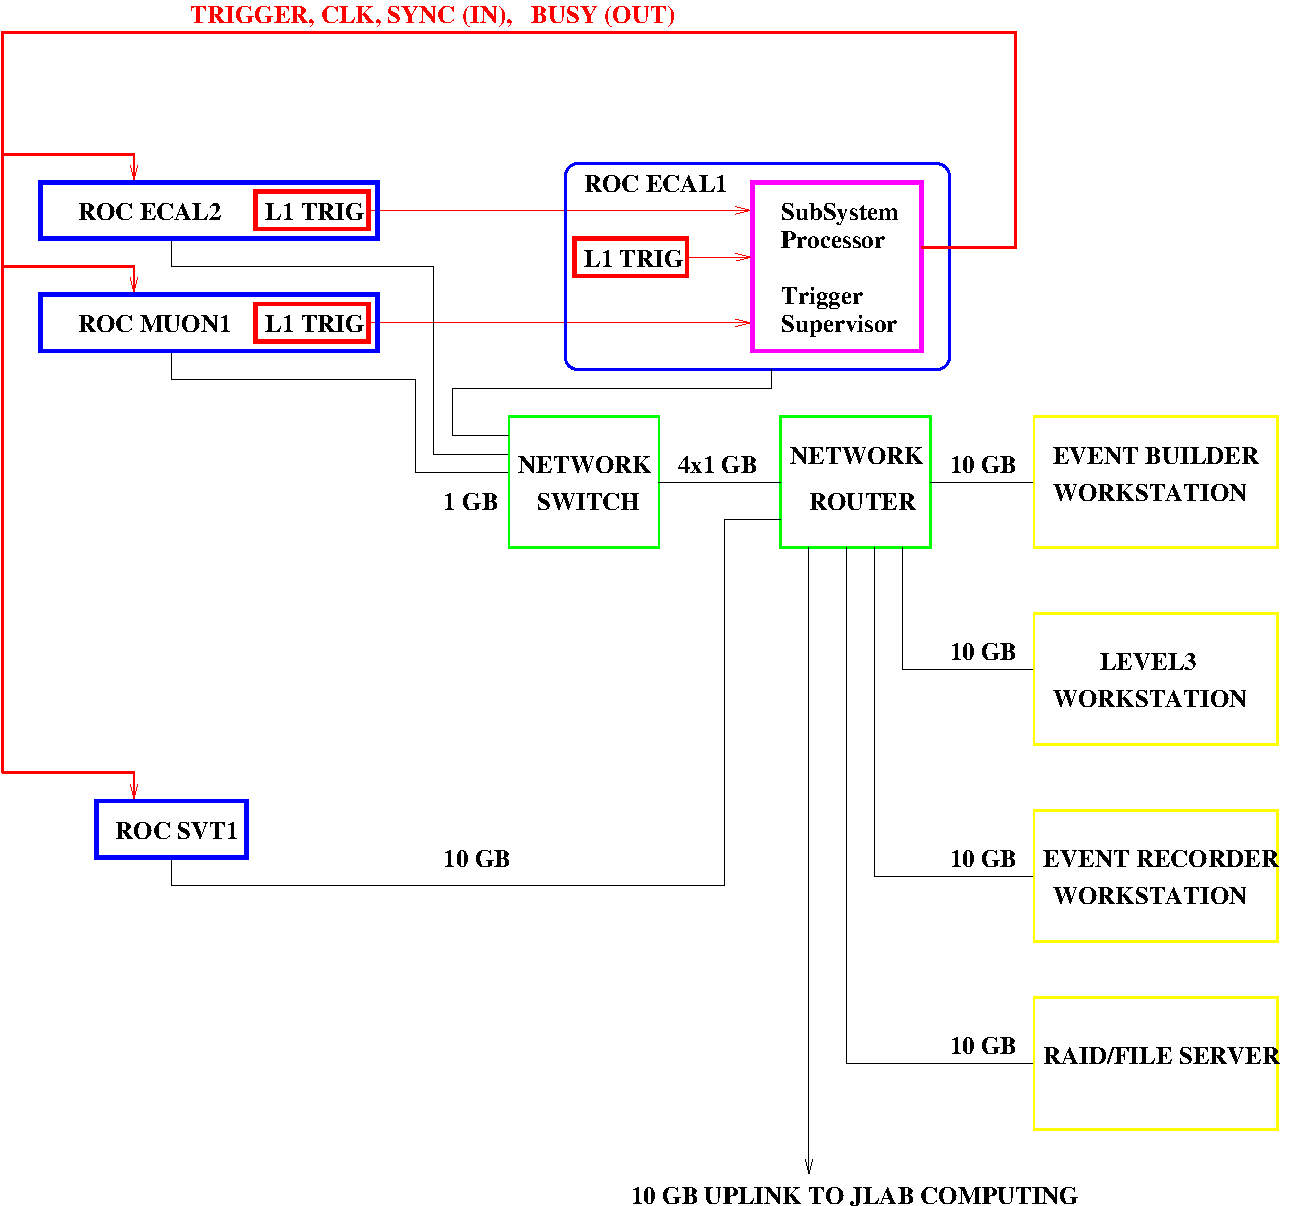
\includegraphics[ scale=0.3]{trigger_daq/figures/daq_schem.pdf}
\caption{\small{Schematic block diagram of the data acquisition system.}}
\label{fig:daq_hardware_overview}
\end{figure*}
The main software component is the Readout Controllers (ROCs) that collects information 
from the front end electronics board, processes it and sends it through the network to the 
Event Builder server. ROCs are installed in every crate holding front end boards. The 
VME based crates runs ROCs on mvme6100 controller boards with prpmc880 or pmc280 
coprocessor modules. {\color{red} Might need update?} The ROC for the SVT runs on 
a processor blade in the ATCA crate which handles the SVT part of the DAQ system. 
The Event Builder assembles 
information from the SVT, ECal and muon detector ROCs and assembles it into a single 
event which is passed to the (RAID5) data storage system capable of handling up to 
100MBytes/s. The Event Builder and other 
critical components run on multicore Opteron-based multi-CPU servers which is a 
sufficient configuration to handle HPS. The backbone of the DAQ network system is a 
Foundry router providing 1Gbit and 10Gbit connections between DAQ components and 
the JLab computing facility. The SVT ROC has a 10Gbit link to the Foundry router while the 
ROCs for the ECal and muon detector connect through a 1Gbit network switch. The long 
term data storage is handled by a 1Gbit uplink to the JLab computing facility. 

Section~\ref{sec:svt_daq} describes the SVT DAQ in more detail. The VXS based readout for 
the ECal and muon detector is described in Sec.~\ref{sec:fadc_daq} and the trigger 
system is explained in more detail in Sec.~\ref{sec:triggerdaq}.

\subsubsection{SVT Data Acquisition}
\label{sec:svt_daq}

\begin{verbatim}
This section needs update including optical readout and power distribution.
\end{verbatim}


The goal of the SVT DAQ is to support the continuous 40MHz readout and processing of signals from 
the 24 silicon strip sensors of the SVT and select those events that were identified by the 
Level 1 trigger system for transfer to the JLab DAQ for further event processing at rates 
close to 50kHz. 
Due to the difficult environment of the SVT with extreme occupancy and pile-up from multiple bunches  the number of noise hits has to be low to keep total data rates under control and 
each pulse from an energy deposition in the silicon needs to be sampled in order to facilitate 
reconstruction of the hit time to high accuracy. 

To meet these demanding requirements each of the 24 silicon strip sensors is connected to a 
hybrid board housing five 128-channel APV25~{\color{red}Reference needed} integrated circuits. The APV25, initially developed for the Compact Muon Solenoid silicon
 tracker~{\color{red}Reference needed}  at the Large Hadron Collider at CERN, was 
 chosen based on their good match to the HPS requirements. They provide amplification, 
 pipelining, and analog storage for trigger accepted events. For each 640-channel hybrid 
 board (shown in Fig.~\ref{fig:hybrid_and_apv25_testrun}
 \begin{figure*}[t]
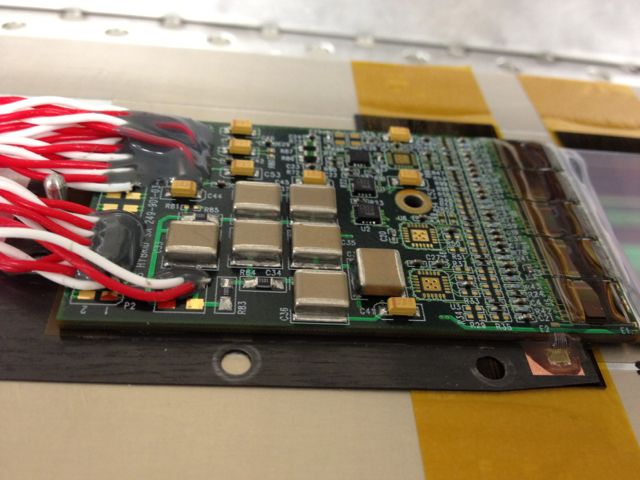
\includegraphics[ scale=0.3]{trigger_daq/figures/hybrid.jpg}
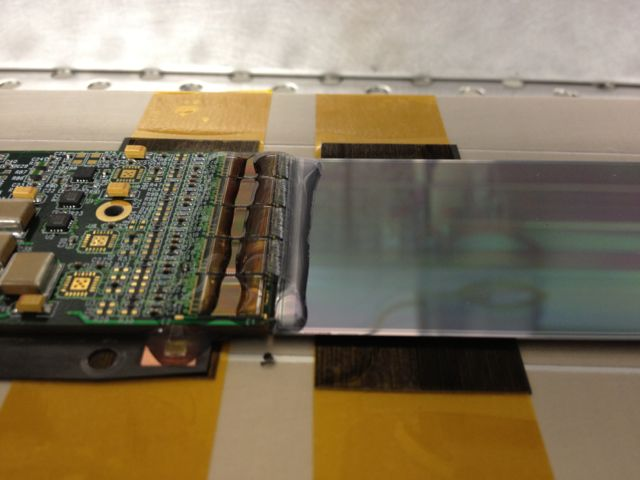
\includegraphics[ scale=0.3]{trigger_daq/figures/apvs-on-hybrid.jpg}
\caption{\small{Picture of a hybrid board from the test run in 2012 holding five 
APV25 ASICs that are wire bonded to the silicon sensor.}}
\label{fig:hybrid_and_apv25_testrun}
\end{figure*}
Each hybrid board has five analog output lines where analog data from each APV25 are 
sent using low power LVDS signals over about 3~m of multi-twisted-pair cable to a readout 
board. 

Figure~\ref{fig:svt_daq_overview} gives an overview of the SVT readout system. 
 \begin{figure*}[t]
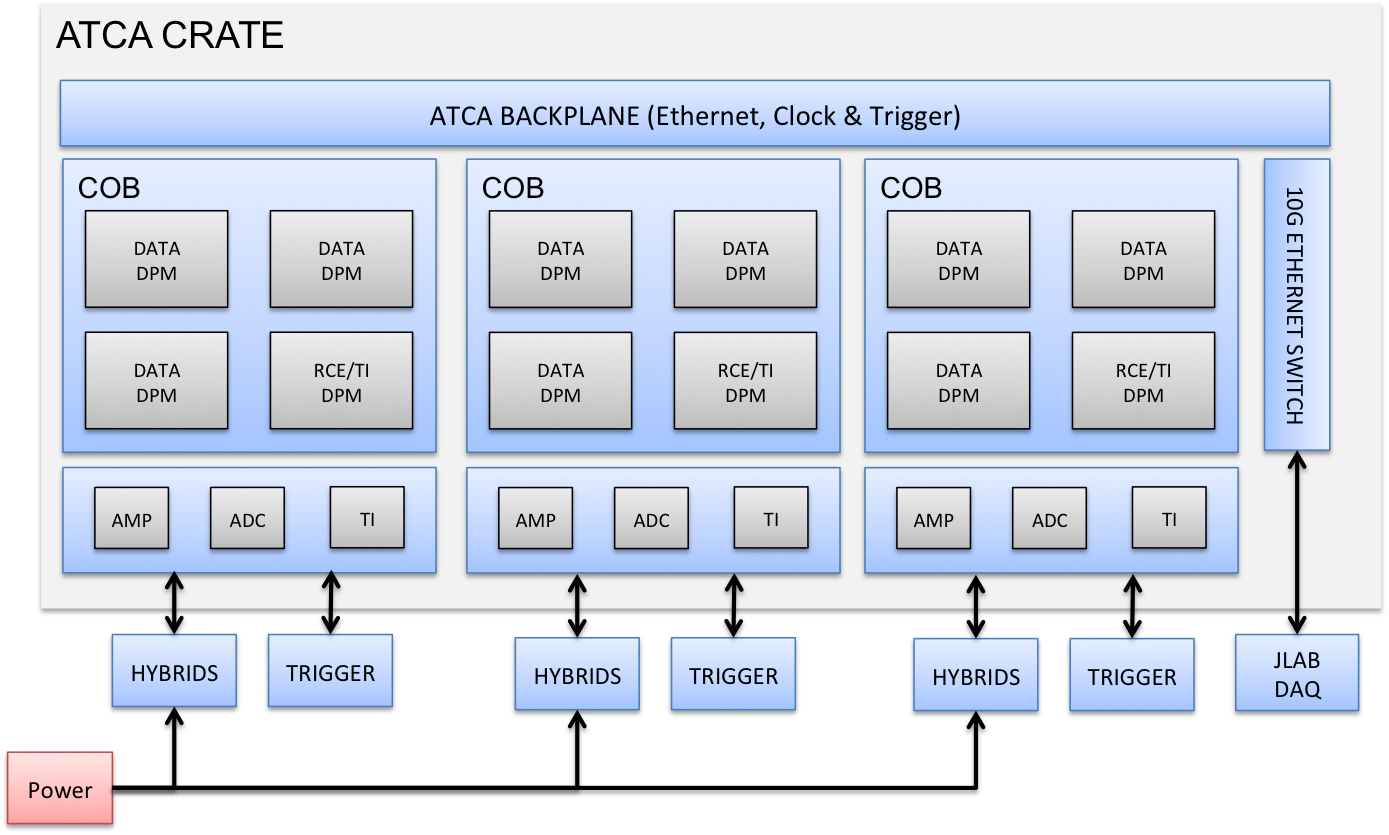
\includegraphics[ scale=0.6]{trigger_daq/figures/svt_daq_schem.png}
\caption{\small{Schematic block diagram of the SVT data acquisition system.}}
\label{fig:svt_daq_overview}
\end{figure*}
It is developed and built at SLAC using the Advanced Telecom 
Communication Architecture (ATCA) system for high speed data transfer. The analog signals 
from the 23,040 channels are digitized on the Rear Transition Module (RTM) boards. A 
pre-amplifier scales the APV25 differential current output to match the range of a 14-bit 
Analog to Digital Converter (ADC). Each RTM board has three sections that each service 
three hybrids. The ADC operates at the system clock frequency of 41.667~MHz. The RTM 
also has a 4-channel fiber optic module to communicate with the JLab trigger supervisor. 
A picture of a RTM board is shown in Fig.~\ref{fig:rtm_testrun}.
 \begin{figure*}[t]
\includegraphics[ scale=0.25]{trigger_daq/figures/rtm.png}
\includegraphics[ scale=0.4]{trigger_daq/figures/svt_daq_module_noted.png}
\caption{\small{Picture of a RTM (top) and COB board (bottom) 
used in the HPS test run 2012.}}
\label{fig:rtm_testrun}
\end{figure*}
The main COB board has four FPGA units that each interfaces with a single section of the 
the RTM.  Each FPGA is housed on a separate daughter board called 
Data Processing Module (DPM). Each DPM receives the digitized signals from the hybrids 
from the RTM, applies thresholds for data reduction and organizes the sample data 
into UDP datagrams. Each DPM also includes an I2C controller to configure and monitor the 
APV25 chips. One of the DPMs functions as the trigger interface which receives trigger 
signals from the optical fiber module on the RTM, handles distribution of clock and trigger 
and handles communication with the JLab trigger supervisor and the RCE. The 
RCE (Reconfigurable Cluster Element) is a generic computational building block 
on the trigger interface DPM running a 450~MHz PPC processor with 4GB of DDR3 
memory. Four COBs housed in a two ATCA crates is sufficient to handle 
the 36 hybrids of the SVT.

The RCE receives and buffers UDP datagrams from the data and trigger DPMs and
 assembles them into full event frames. The RCE also runs an implementation of the JLab ROC application that handles the integration of the SVT event frames into the JLab DAQ 
 system described above. The RCE node transfer data to the JLab DAQ  
 through a 10~Gbit Ethernet backend interface. 

The readout rate of the SVT is 43kHz, limited by the APV25 readout rate. 
%The maximum readout rate of the SVT DAQ  is limited by the readout time 
%of the APV25 chip. Using overlapping trigger and readout functionality, where the 
%APV25 chip can buffer up to 5 triggers, the maximum average readout rate expected for 
%HPS is 45kHz {\color{red} need verification}.   







\subsubsection{ECal and Muon Detector FADC Readout}
\label{sec:fadc_daq}
The main part of the readout of the ECal and muon detector are identical. Signals from each 
readout unit are sent to a signal splitter. For the ECal the charge signal from the APDs are 
shaped and amplified as described in Sec.~\ref{sec:ecal_readout} before feed into the 
splitter. One of the outputs of every splitter (for both the ECal and muon detector channels) 
feeds a separate channel on Flash ADC (FADC) readout boards that are packaged in 
16-channel VXS modules. Two VXS modules are used to accommodate the two ECal 
halves, each one with 221 channels, and a single VXS module is used to readout the muon 
detector. 

The FADCs stores the 12-but digitized samples of each channel in 8~$\mu$s deep pipelines. 
After a trigger is received a part of the pipeline corresponding to X number of samples 
before and Y samples after the signal passed a predefined threshold. Transferring only 
the time it passed threshold and a channel sum as energy estimate greatly reduces the data rate. 


The FADCs are an integral part of the HPS calorimeter trigger system. Pulse energies 
and times from each FADC channel in the same VXS crate is collected by a crate trigger
 processor which performs cluster finding. The result from each create trigger processor (i.e. each half of 
the ECal) is combined in the sub-system processor module which applies further selections 
based on single- and combination of clusters to form a trigger decision passed to the trigger 
supervisor. The trigger process has a pulse timing resolution of 4~ns. This allows a narrow 
coincidence window of 8~ns to be used when searching for clusters. 
This is an important part of improving 
the pattern recognition to reduce confusion in the tracker which has considerable longer 
integration times. 


See Sec.~\ref{sec:triggerdaq} for more details on the operation of the trigger system.


\subsubsection{Trigger System}
\label{sec:triggerdaq}

%\subsubsection{ECal Trigger overview}


The proposed trigger system is nearly deadtimeless. The trigger decision goes to the Trigger Supervisor every 4 ns. The trigger supervisor can apply deadtime if necessary, for example on a 'busy' or 'full' condition from front-end electronics.


\begin{figure}[t]
\includegraphics[scale=0.5]{daq_trigger/figures/FADC250_Photo_001.jpg}
\caption{\small{Jefferson Lab FADC250 VXS module.}}
\label{fig:fadc}
\end{figure}

The information from top and bottom parts of the ECal will be sent to the Jefferson Lab FADCs (Flash Analog-to-Digital Converters), Fig.~\ref{fig:fadc},  located in two different VXS crates (see Fig.~\ref{fig:hps_trigger_cal}). FADC  works at the frequency 250~MHz; i.e. it measures the amplitude of each ECal channel every 4 ns. FADC has 12bit pulse digitizer for readout and trigger processing. 

The first stage components of the trigger logic are incorporated into the Flash ADC board's FPGAs, while the final decision is made in a Crate Trigger Processors (CTPs) and  Sub-System Processor (SSP) .
FADC sends the information about the pulse energy and time to CTP.


\begin{figure}[t]
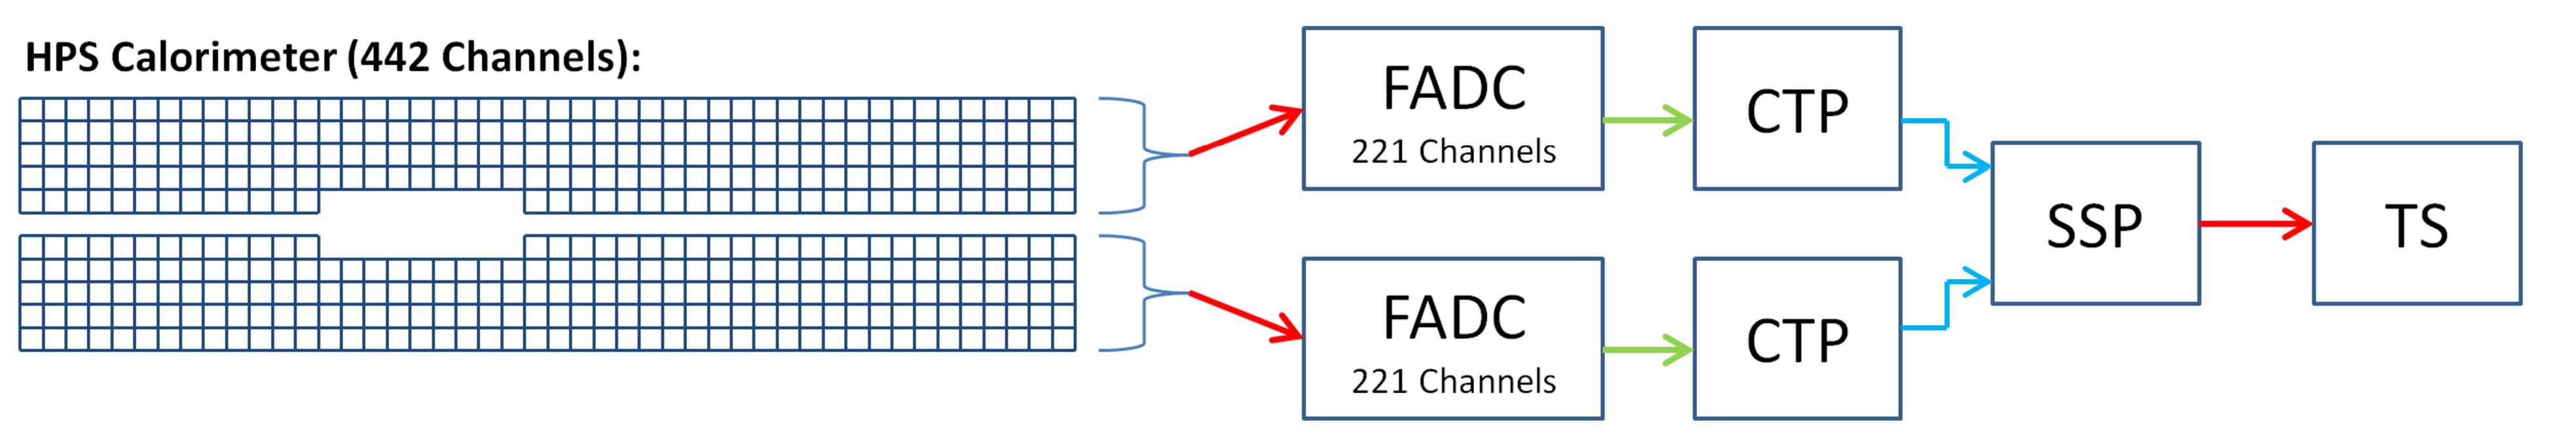
\includegraphics[scale=0.25]{daq_trigger/figures/hps_trigger_cal}
\caption{\small{ECAL trigger logic. FADC - Jlab Flash ADC, CTP - Crate Trigger Processor, SSP - Sub-System Processor, TS - Trigger Superviser.}}
\label{fig:hps_trigger_cal}
\end{figure}

The trigger system can be broken down into the following 3 sections:
 \begin{itemize}
 \item FADC (pulse finding): Samples the detector channel to find pulses. Pulse energy and times are sent to CTP.
 \item CTP (cluster finding): Searches FADC pulses (from half of calorimeter) to find clusters. Cluster energy, time, and hit pattern sent to SSP.
 \item SSP (cluster pair finding): Searches CTP clusters (from top and bottom) to find cluster pairs and create the trigger. Trigger cuts on pairs decide final trigger.
 \end{itemize}
 
 Trigger logic will search for a time coincidence between two clusters in opposite halves of ECal that occur within a programmable time window with 4ns resolution. The maximum trigger decision time (latency) is currently set to 3 $\mu$s for Level 1. That value is defined by the SVT readout APV25 chip.

The Trigger Supervisor generates all necessary signals, and controls the entire DAQ system readout through the Trigger Interface units. The Trigger Interface (TI) units installed in every crate participate in the readout process. The system is free-running and driven by a 250MHz global clock. The maximum trigger accept rate is 50 KHz.



%\subsubsection{Crate Trigger Processor} 

The Crate Trigger Processor receives the energy pulses (in MeV) and time stamp from each FADC channel in the crate (see Fig.~\ref{fig:hps_trigger_3x3}).
The algorithm used for cluster finding makes use the parallel processing nature of FPGAs by simultaneously searching for 125 clusters up to 3x3 in size across the calorimeter crystal array.  
A Cluster Processor (CP) algorithm:

\begin{itemize}
\item Add energy from hits together for every 3x3 square of channels in ECal
\item Hits are added together if they occur (leading edge) within a programmable number of clock cycles of each other (4 ns steps)
\item If 3x3 energy sum $\ge$  the programmable cluster energy threshold CTP reports cluster to the Sub-System processor the cluster parameters (time, energy, position and 3x3 hit pattern. 
\end{itemize}

Every 4ns the CTP evaluates all hits in its half of the calorimeter. A programmable time window is used to allow hits that are out of time with each other be considered as part of a cluster sum. This is done by reporting hits when they occur and then reporting them again for the next N number of 4 ns clock period, where N can be 0 to 7. This is useful to deal with skew and jitter that develop from the detector, cabling, and electronics.

When the sum of all hits in the 3x3 window occurring in a programmable time window are greater than the programmable energy threshold the cluster processor will report this cluster to the SSP if the energy is greater than all neighboring (up, down, left, right, and diagonals) 3x3 window cluster energies for that clock cycle. If the energy is not greater than its neighbor it will not be reported, but the neighbor will report if it is the greatest. The reason for this filtering is because there are several 3x3 windows that overlap and see the sample crystals and also many physics single clusters are larger than a 3x3 window.

The reported clusters to the SSP contain:

\begin{itemize}
\item 13bit Cluster energy (MeV)
\item Cluster position (crystal index: x,y)
\item Cluster time (4ns resolution)
\item Cluster hit pattern 3x3 (detector channels reporting a hit in the cluster)
\end{itemize}

The cluster position is the coordinate of the cluster processor that reported the cluster, which is where the peak cluster energy was seen from a 3x3 view. The 3x3 cluster hit pattern can be used by the SSP to help filter strange cluster patterns and/or make a low resolution cluster centroid computation.

\begin{figure}[h]
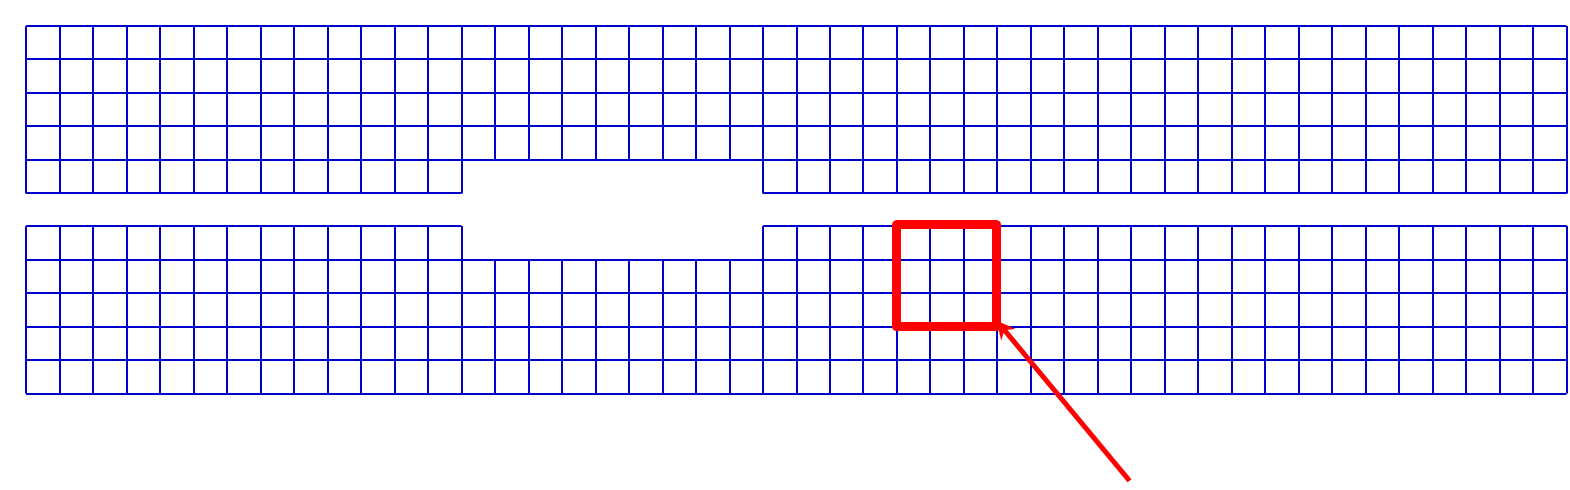
\includegraphics[scale=0.4]{daq_trigger/figures/hps_trigger_3x3}
\caption{\small{Cluster finding algorithm.}}
\label{fig:hps_trigger_3x3}
\end{figure}




%\subsubsection{Sub-System Processor} 

The cluster's time, energy, position and 3x3 pattern found in two VXS crates are reported to the Sub-System Processor. 
The SSP collects the cluster information from the full calorimeter and can create the trigger decisions of two types:
single cluster trigger and multi-cluster triggers.
Single cluster trigger condition includes the check on the cluster energy, $E_{min}\le E_{cluster}\le E_{max}$, where $E_{min}$ and $E_{max}$ are programmable minimum and maximum cluster energy.

Pairs trigger includes more conditions
\begin{itemize}
\item Energy sum,  
$E_{min}\le E_{top}+E_{bottom}\le E_{max}$
\item Pair time coincidence, 
$|t_{top}-t_{bottom}|\le \Delta t_{max}$ 
\item Energy difference, 
$|E_{top}-E_{bottom}|\le \Delta E_{max}$ 
\item Energy slope,
$E_{cluster\_with\_min\_energy}+R_{cluster\_with\_min\_energy}\times F_{energy}\le Threshold_{slope}$
\item Co-planarity, 
$|
tan^{-1}(\frac{X_{top}}{Y_{top}})-
tan^{-1}(\frac{X_{bottom}}{Y_{bottom}}) |\le Coplanarity_{angle}$
\item Number of hits in 3x3 window, 
\#$hits_{3\times 3}\ge HitThreshold$
\end{itemize}
\noindent
where $ E_{max}$,  $\Delta t_{max}$, $ \Delta E_{max}$ , $Threshold_{slope}$, 
$F_{energy}$, $Coplanarity_{angle}$
and
$HitThreshold$ are programable parameters.


Online event analysis will be provided to be compared against trigger event data for immediate verification (on each trigger cut: cluster energies, positions, timing, energy slope, coplanarity and hit threshold). With identical ADC readout and trigger pulse processing and high energy resolution, very precise agreement can be expected between trigger and readout.





%\subsubsection{Diagnostic Tools}

The previous experience with the similar (but much more simpler) trigger system showed that diagnostic tools are necessary to make sure that the calorimeter and trigger electronics work as expected. 

Scalers will be implemented for every ECal channel. The example of this diagnostic tool is presented in Fig.~\ref{fig:dvcs_beam}
from the previous version of the calorimeter. Hot or dead channels are easily identified online.
\begin{figure}[h]
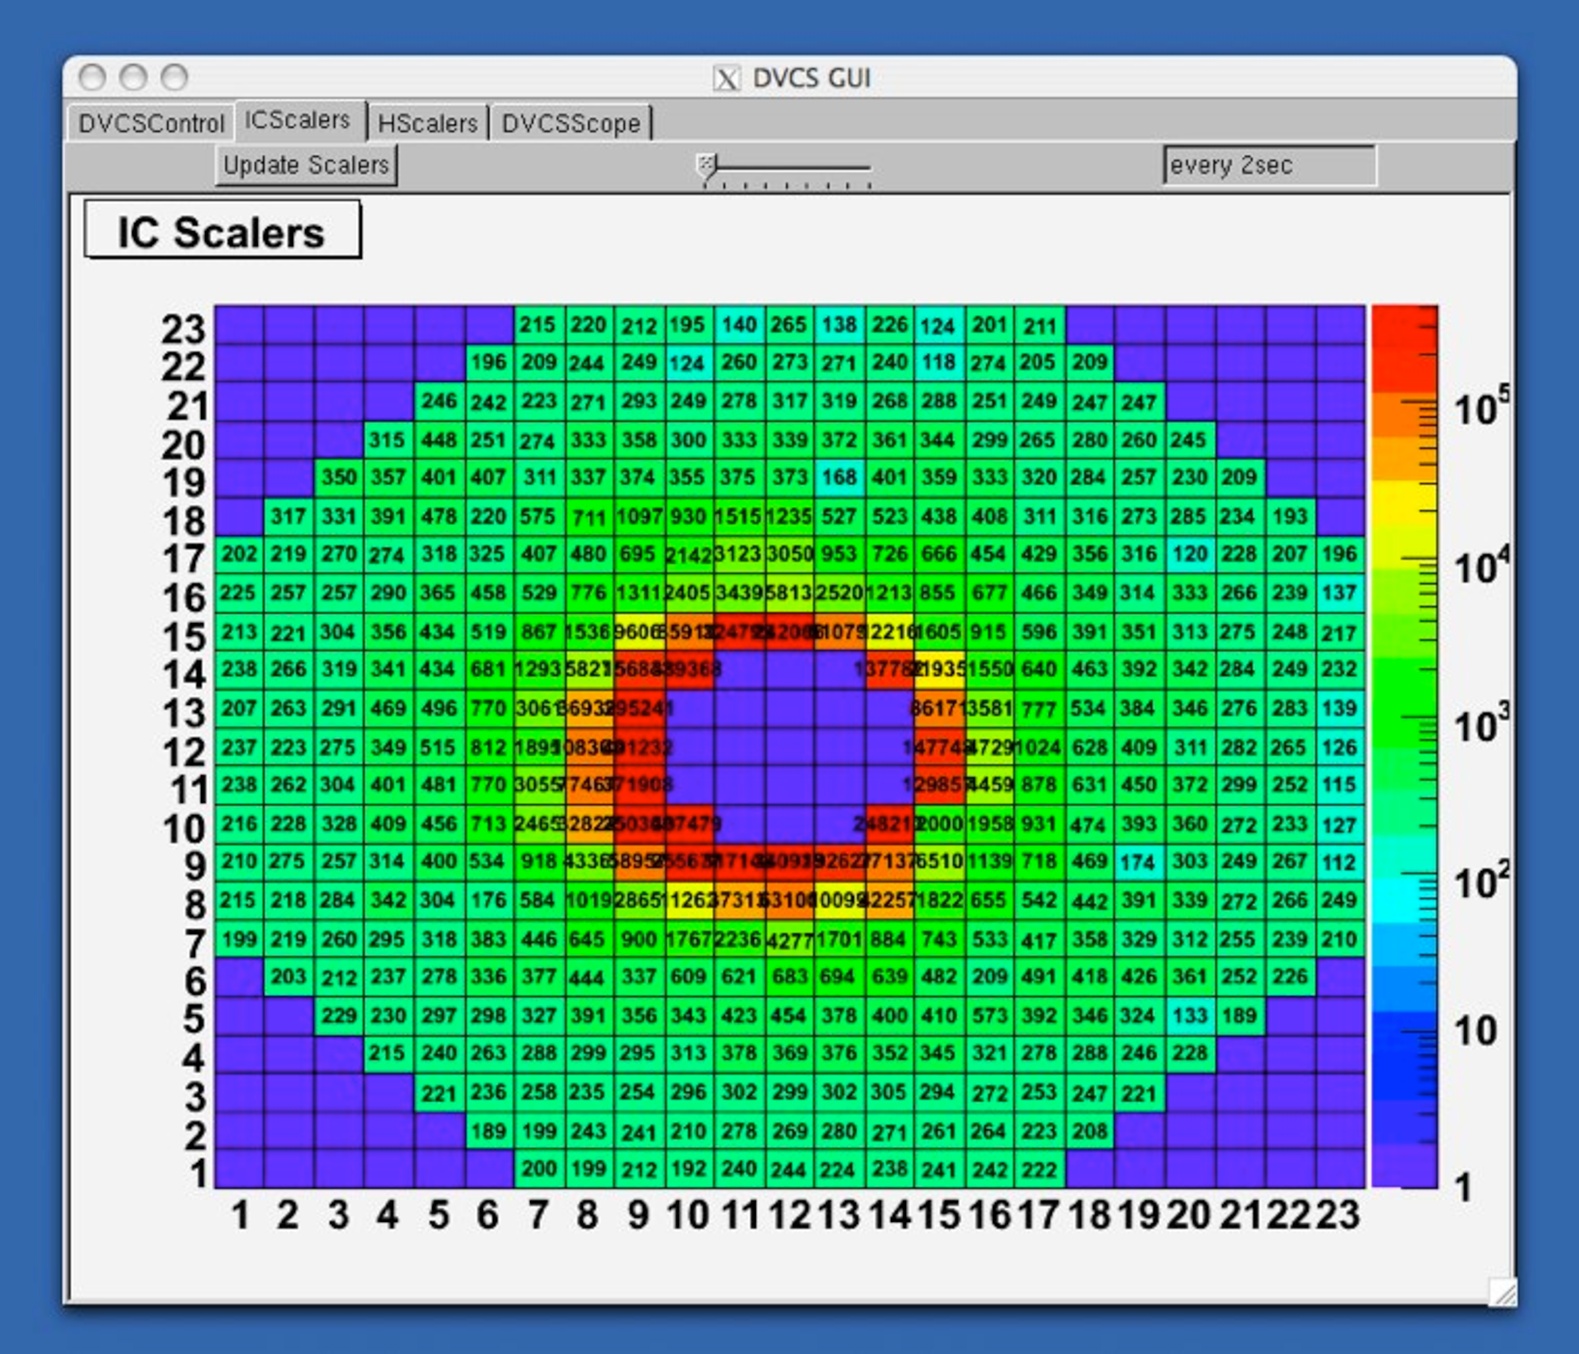
\includegraphics[scale=0.6]{daq_trigger/figures/dvcs_beam}
\caption{\small{Scalers (example from the previous version of the calorimeter).}}
\label{fig:dvcs_beam}
\end{figure}
Diagnostic scope permits to analyze on-line  the trigger logic. The goal to have  the Two-Dimensional Analyzer
 is to provide a remote debug interface to identify bad channels, verify cluster finding algorithms and check timing.
 The details of this analyzer are as following:
 
\begin{itemize}
\item Logic analyzer runs in parallel, non-intrusive, to the calorimeter trigger
\item Can setup trigger on any ECal pixel arrangement and/or cluster count
\item Can move forward/backward in time by ~250 ns to see timing details
\item Will be customize for HPS geometry and hardware
\end{itemize}

The example of the 2D analyzer is presented in Fig.~\ref{fig:dvcs_2_cluster}. Two clusters are displayed
in the picture. The red color displays the hits in the calorimeter and  the center of clusters is displayed in yellow.

In addition to the scalers, the distributions on individual ADC channel pulse energy will be provided.
The cluster hits positions and energy from SSP processor will be histogrammed as well. Two histograms (accepted and rejected) will be provided for each trigger cut used in the trigger logic.



\begin{figure}[t]
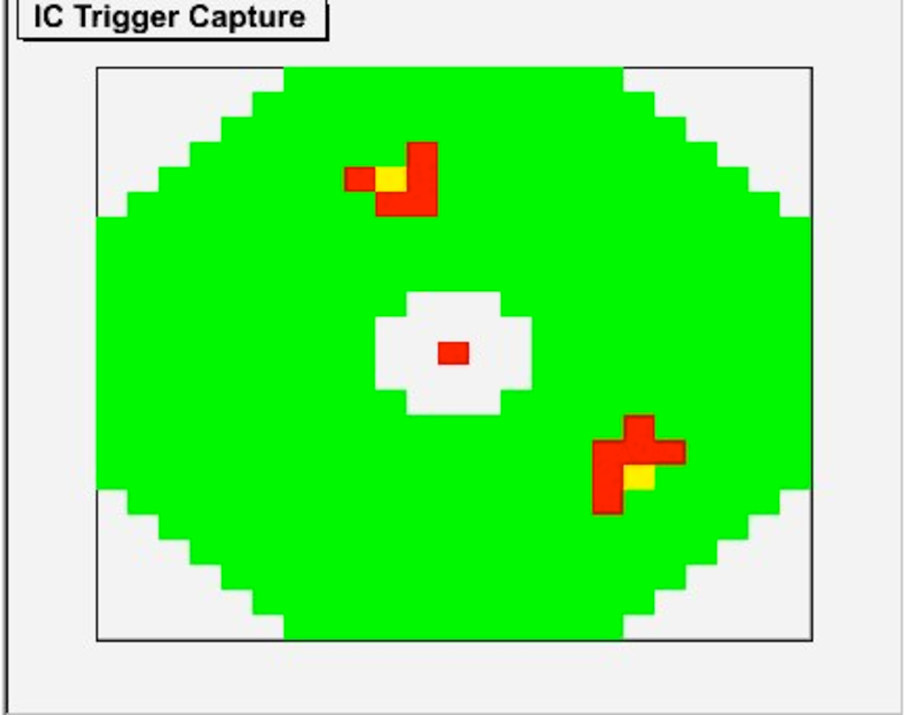
\includegraphics[scale=0.8]{daq_trigger/figures/dvcs_2_cluster}
\caption{\small{Diagnostic scope (example with two clusters found from the previous version of the calorimeter). Green - no hits, red - tower with hit, yellow - cluster found.}}
\label{fig:dvcs_2_cluster}
\end{figure}






%\subsubsection{Muon Trigger}

A muon detector composed of a four iron absorbers  and four double-layer scintillator planes, positioned after each absorber. Similar to the Ecal, the muon detector will consist of two halves, one above and one below the beam.
GEANT4 simulations have been used to study the trigger rates in the muon system due to background hits. It is expected that the true di-muon rate will be quite small compared to the ECal trigger rate and should not cause problem for the DAQ. 
A total of 144 readout channels are needed (9x16 channels multi-anode PMTs). Signals from each channel will be sent to a TDC and to a FADC. The FADC information will be used to construct the muon trigger. The TDC information together with information from FADC will be used in offline analysis to measure the hit position along the strip.

Selecting coincidence hits with MIP energy deposition in at least three layers of the scintillation hodoscope will identify muons. 
The muon trigger logic has to find one track in the top part of the detector in coincidence with another track in the bottom part of the detector. The track finding algorithm can be easily realized in the FPGA logic of the muon Crate Trigger processor.



\subsubsection{Event Size and Data Rates}

{\color{red}This needs to be updated with the latest occupancy values.}

The extreme radiation environment with tails of scattered beam imposing high occupancy
 puts strict requirements on high readout speed but consequently low noise readout to limit 
 the data rates. The event sizes and rates are based on estimates from detailed simulations 
 verified by measurements in the test run. 
  
As suggested in Sec.~\ref{sec:svt_desc}, the SVT will be operating at an effective threshold of three
times the noise level or an equivalent of 0.135\% occupancy. This translates to on average of 21 channels above threshold. Background studies (see Sec.~\ref{sec:hps_perf}) show that 
there are on average 10 tracks per event at a beam energy of 2.2~GeV and current of 
200~nA. With each track 
having on average 2 strips above threshold for each sensor there are on average 160 channels above threshold. Each of these channels will result in six digitized samples of the 
pulse shape giving in total of 1084 samples per event for the SVT.
Each channel has, in addition to the digitized samples,  header information that identifies the 
the channel number and it's chip address. The complete SVT event size also 
include the overhead from each FPGA and the JLab data stream bank header.  
With the average occupancy 
estimated above the expected event size is 3.6~kbytes corresponding to a data rate of 
approximately 155~Mbytes/s assuming an average trigger rate of 43~kHz.  
This high data rate is handled utilizing 
the 10~Gbit ethernet connections internally of the ATCA crate and also to the JLab DAQ.
{\color{red} (need to update these with the exact simulation of environment}


The data rate from the ECal and muon system is estimated from the same running 
conditions as the SVT above. 
Each each calorimeter or muon hit consist of 8 bytes (4 byte energy, 4 byte time)
 with a 12 byte header (4 byte trigger number, 8 byte trigger time) for each FADC board. 
 The main limitation is of the order of 100Mbytes/s from each VXS crate. For a 
 10\% occupancy estimated in Sec.~\ref{sec:trig_rate} the ECal event size is approximately 0.7~kbytes which translates to a total data rate of approximately 31.5~Mbytes/s 
(split between the two VXS crates), well within the DAQ system design. 

The contribution from the muon system is small due to it's significantly lower number of channels. The system is readout by nine FADC boards in a single VXS crate. The event 
size for a 10\% occupancy level is 0.2~kbytes which translates to a data rate of 10~Mbytes/s. 

Table~\ref{tab:data_rates} summarizes the event size and data rates for the different 
sub-systems. 
\begin{table}[]
\centering
\begin{tabular}{l|c|c|c}
Sub-system & Occupancy(\%) & Event size (kB) & Data Rate (MB/s) \\
\hline
SVT & 0.135 & 4.5 & 203 \\
ECal & 10 & 0.7 & 32 \\
Muon & 10 & 0.2 & 10 \\
\hline
Total & - & 5.4 & 245 \\
\hline
\end{tabular}
\caption{{\small Occupancy, event size and data rate expected for beam energy of 2.2~GeV and a current of 200nA.} {\color{red}Need update}}
\label{tab:data_rates}
\end{table}
The dominant contribution comes from the SVT where irreducible real hits from the high occupancy is dominating the rates. Using high-speed data links it's still within the DAQ system and high performance RAID file servers it's within the the system design. 

The total data volume for a 2 week long production run is expected to be around 83Tb 
assuming a duty factor of 30\%.  For a longer run a Level~3 fast track trigger can 
be deployed to lower the data rates and total volume to be written to disk. 


\subsection{Offline Computing Model}

The following is an outline of the offline computing model envisioned for satisfying the analysis needs of the HPS experiment. The raw data collected over the running periods must be processed through calibration passes, reconstructed into calibrated objects useful for analysis and separated into analysis streams. Corresponding Monte Carlo will also need to be produced and separated into the same analysis streams.

Table~\ref{tab:data_volume} shows the expected number of triggered events and
%the average trigger rate and 
the total amount of data expected over the 
different runs. For the six weeks long run in 2014 we expect to collect approximately 223~TB of raw data. 
We assume that the experiment collects data for all of its available beam time and the time allocated for detector commissioning, even though the experiment reach only assumes 50\% availability; this gives a conservative estimate of computing requirements.
\begin{table}[]
\centering
\begin{tabular}{|l|c|c|c|c|c|c|}
\hline
Run & $E_{beam}$ (GeV) & Time (days) & Events ($\times 10^9$) & Raw data (TB) & Processed data (TB)\\
\hline
2014 & 1.1 & 21 & 33 & 100 & 455 \\
2014 & 2.2 & 21 & 29 & 63 & 393  \\
%2014 & 6.6 & 14 & 15 & 55 & 209  \\
\hline
Total & - & 42 & 62 & 163  & 848 \\
\hline
%2015 & 1.1 & 30 & 47 & 171 & 650 \\
2015 & 2.2 & 35 & 48 & 105 & 655 \\
2015 & 6.6 & 35 & 38 & 76 & 522 \\
\hline
Total & - & 70 & 86 & 181 & 1177 \\
\hline
\end{tabular}
\caption{{\small Summary of the raw and processed data expected from the HPS runs. }}
\label{tab:data_volume}
\end{table}
The raw data must be processed to produce physics data objects that can be analyzed. This reconstruction process will also include filters to select events of physics interest. We use the event size estimates in \ref{tab:data_rates} for raw data, and an event size of 13.7 kB for reconstructed data.

%in Table~\ref{tab:raw_data_size}. 
%\begin{table}[]
%\centering
%%\begin{tabular}{|l|c|}
%\hline
%Type & Event size (kB) \\ 
%\hline
%Raw (EVIO)  &  3.6 \\
%\hline
%Reconstructed LCIO & 13.7 \\
%\hline
%\end{tabular}
%\caption{{\small Data event sizes. }}
%\label{tab:raw_data_size}
%\end{table}

For modeling signals, estimating backgrounds and confirming the understanding of the detector 
performance, extensive Monte Carlo simulation is needed. Table~\ref{tab:mc_event_size} summarizes 
the typical event size at the various stages of the simulation. 
\begin{table}[]
\centering
\begin{tabular}{|lccc|}
\hline
Event type & Sim. stage & Size/triggered event (kB) & Mass points  \\
\hline
Beam bkg.  & evgen	& 37.0	& 1	\\
A' signal & evgen	& 0.5	& 10	\\
A'+beam bkg & evgen	& 37.4	& 10	\\
\hline
Beam bkg.  & MC output	& 79.5	& 1	\\
A' signal & MC output	& 2.5	& 10	\\
A'+beam bkg & MC output	& 82.0	& 10	\\
\hline
\end{tabular}
\caption{{\small Event sizes in kB per triggered event, including pileup events for beam background. }}
\label{tab:mc_event_size}
\end{table}

%\begin{table}[]
%\centering
%\begin{tabular}{|lccc|}
%\hline
%Event type & Sim. stage & Size/500k bunches (MB) & Mass points  \\
%\hline 
%A' signal & evgen & 22 & 10  \\
%Beam bkg. (incl. brems. events) & evgen & 331 & -\\ 
%Trident bkg. & evgen & 139 & - \\
%\hline
%Total & evgen & 431 & -\\
%\hline
%A' signal & Merged evgen & 134 & 10 \\
%Beam bkg. & Merged evgen & 141 & - \\ 
%Trident bkg. & Merged evgen & 134 & - \\
%Beam+trident bkg. overlay & Merged evgen & 187 & - \\ 
%A'+Beam+trident bkg. overlay & Merged evgen & 233 & 10 \\ 
%\hline
%Total & Merged evgen & 829 & - \\
%\hline
%A' signal & Reco. LCIO  & 284 & 10 \\
%Beam bkg. & Reco. LCIO  & 366 & - \\ 
%Trident bkg. & Reco. LCIO  & ???284??? & - \\
%Beam+trident bkg. overlay & Reco. LCIO  & 379 & - \\ 
%A'+Beam+trident bkg. overlay & Reco. LCIO  & 383 & 10 \\ 
%\hline
%Total & Reco. LCIO  & ??? & - \\
%\hline
%\end{tabular}
%\caption{{\small Event sizes in MB per 500k simulated bunches. }}
%\label{tab:mc_event_size}
%\end{table}
%LCIO
%Beam bkg plus trident: 379 Mb per 500,000 bunches
%Beam: 366 Mb per 500,000 bunches
%AP/Beam/Trident: 383 Mb per 500,000 bunches at 7 different masses
%Ap: 284 Mb per 500,000
%
%Merged StdHep:
%Beam bkg plus trident: 187 Mb per 500,000 bunches
%Beam: 141 Mb per 500,000 bunches
%AP/Beam/Trident: 233 Mb per 500,000 bunches at 10 different masses
%Ap: 134 Mb per 500,000 bunches at 10 different ap masses
%Trident: 134 Mb per 500,000 bunches
%
%Raw StdHep: 
%Ap: 22 Mb per 500,000 bunches at 10 different ap masses
%Beam: 270 Mb per 500,000 bunches + an additional 61 Mb for brem events (500,000?)
%Trident: 139 Mb per 500,000 bunches
In total approximately 1/10th of the number of data events collected need to be simulated. For the 2014 run this amounts to 6.2 billion events.
In addition, 100 million A' events must be simulated at each of 10 mass points at each beam energy. This totals 2 billion A' events.

% storage description
In total 1975 (2602)~Tb of storage for data is needed for the 2014 (2015) run.
%(17600+15800+12600)*86400*14/500000*383*1e6/1e12=42,6215
%                     #events/bunches*size in Mb*1M/1T= 

Tape is currently the only economical storage
solution for storing all of the raw, simulated and processed data.
The processing of the raw data is foreseen to occur at JLAB. Given a
typical bandwidth between sites of 3 to 4 Tb/day, analyses needing
access to the hit level information will need to be run at JLAB or run
on small samples of exported data unless they can take advantage of the
analysis streams. Analysis streams of events satisfying
pre-selections criteria for targeted analyses will be exported to remote
sites. Likewise, the simulated data is foreseen to be processed at the
remote sites and the equivalent analysis streams for the simulated data
will be used for sharing among the sites. In addition, disk space will be 
needed for ntuples, code releases, and scratch areas and approximately 10\% of the 
processed data. To accommodate this, ???80(171)~TB??? will be needed for the 2014 (2015) run. 
The HPS storage requirements are summarized in Tab.~\ref{tab:datastorage}.
\begin{table}[tbp]
\centering
\begin{tabular}{|l|c|c|}
\hline
Storage category & 2014 (TB) & 2015 (TB) \\
\hline
Raw data & 163 & 181 \\
Processed raw data & 774 & 1658 \\
Simulated data & 1025 & 1776 \\
\hline
Total tape space & 1975 & 2602 \\
\hline
%90days/42days*43Tb = 92Tb
Disk space  & ???80???  & ???171??? \\
\hline
\end{tabular}
\caption{{\small Data storage summary.}}
\label{tab:datastorage}
\end{table}
%(17600+15800+12600)*86400*14=55641600000 events
%(17600+15800+12600)*86400*14*0.1/3600}=1545600 cpu hours


%cpu requirements
Approximately 0.1~CPU seconds are needed to reconstruct a data event on 
a typical 2.4~GHz core. This would require a total of 1.7 million CPU hours of processing for the 
entire 2014 dataset at the JLab processing center.  To simulate events, approximately 0.02 CPU seconds 
are needed for a beam event and approximately 0.7 seconds for an A' event. In total 1.1 million CPU hours is needed for Monte Carlo 
simulation which will be shared between SLAC and JLab. 
Based on experience with previous experiments, it is reasonable to estimate that the net CPU needed for 
analysis work (batch and interactive) will be comparable to that needed for production. We expect 
that this will be shared relatively evenly between JLab and SLAC. The HPS offline computing requirements 
are summarized in Tab.~\ref{tab:computing}.
\begin{table}[tbp]
\centering
\begin{tabular}{|l|c|c|}
\hline
Computing category & 2014& 2015 \\
\hline
Raw data processing ($\times 10^{6}$~CPUh)  & 1.7 & 2.4 \\
Simulation production ($\times 10^{6}$~CPUh) & 1.1 & 1.1 \\
\hline
Total ($\times 10^{6}$~CPUh) & 2.8 & 3.5 \\
\hline
\end{tabular}
\caption{{\small Computing needs summary.}}
\label{tab:computing}
\end{table}


%\clearpage
\section{May-2012 Test Run {\it Pelle}}
\label{sec:testrun2012}
The HPS Test Run was proposed to DOE early in 2011 as the first stage of the HPS experiment. Its
purposes included demonstrating that the apparatus and data acquisition systems would work well,
that the trigger rates and occupancies to be encountered in electron-beam running were as simulated,
and that the apparatus would performed as needed to conduct the HPS experiment. It would also
provide valuable experience to the HPS Collaboration in all aspects of designing, building, installing,
and running the experiment at JAB. It was hoped that the experiment would get dedicated run time
in an electron beam and even, if things performed as expected, that HPS could begin its search for
heavy photons. The HPS Test Run was installed on April 19, 2012, and ran parasitically with the HDice
experiment, using a photon beam, until May 18. The JLAB run schedule precluded any dedicated
electron beam running, but the HPS Test Run did get some valuable dedicated photon beam running.

This section briefly reviews the HPS Test Run apparatus, which is a simplified version of the apparatus
described above for the full HPS experiment, and demonstrates the feasibility of the detector
technologies proposed for silicon tracker, ECal, and data acquisition systems. It documents the
performance of the trigger, data acquisition, silicon vertex tracker, and electromagnetic calorimeter
and shows that the performance assumed in calculating the physics reach of the experiment is realistic.
Of particular importance, data from the dedicated photon beam running has been used to compare
the observed trigger rates with that expected in simulation. The trigger rate is almost entirely due to
photons which have converted to e$^+$e$^-$ upstream of the HPS trackers, and is sensitive to the multiple
Coulomb scattering of the electrons in the conversion target. Good agreement between data and
simulation confirm the EGS5 simulation and its description of multiple Coulomb scattering. Since
multiple Coulomb scattering of the electron beam dominates the SVT occupancies and ECal trigger rates
in HPS, confirming the simulation has demonstrated that backgrounds in HPS are understood.

In addition to the important test of our simulation tools, the HPS parasitic tests, staged over the Hall-B HDice run (g14), accomplished the following: 
\begin{enumerate}
\item  integrated SLAC and JLAB readout systems into a single DAQ
\item fully tested the Level 1 trigger system based on FADCs
\item tested experimental monitoring and controls
\item gained experience with running the test apparatus, in particular running SVT in vacuum
\end{enumerate}

\subsection{HPS Test Run Apparatus } 

In Figure \ref{fig:hpstest_layout}, the layout of the parasitic run is shown. The silicon vertex tracker was installed inside the Hall B pair spectrometer magnet vacuum chamber. The electromagnetic calorimeter was mounted downstream of it.
Both the Si-tracker and the ECal were retracted off the beam plane to allow clean passage of the photon beam through the system, and also not to obscure converted (e$^+$e$^-$) pairs from being detected in the PS hodoscopes.
 
\begin{figure}[ht]
    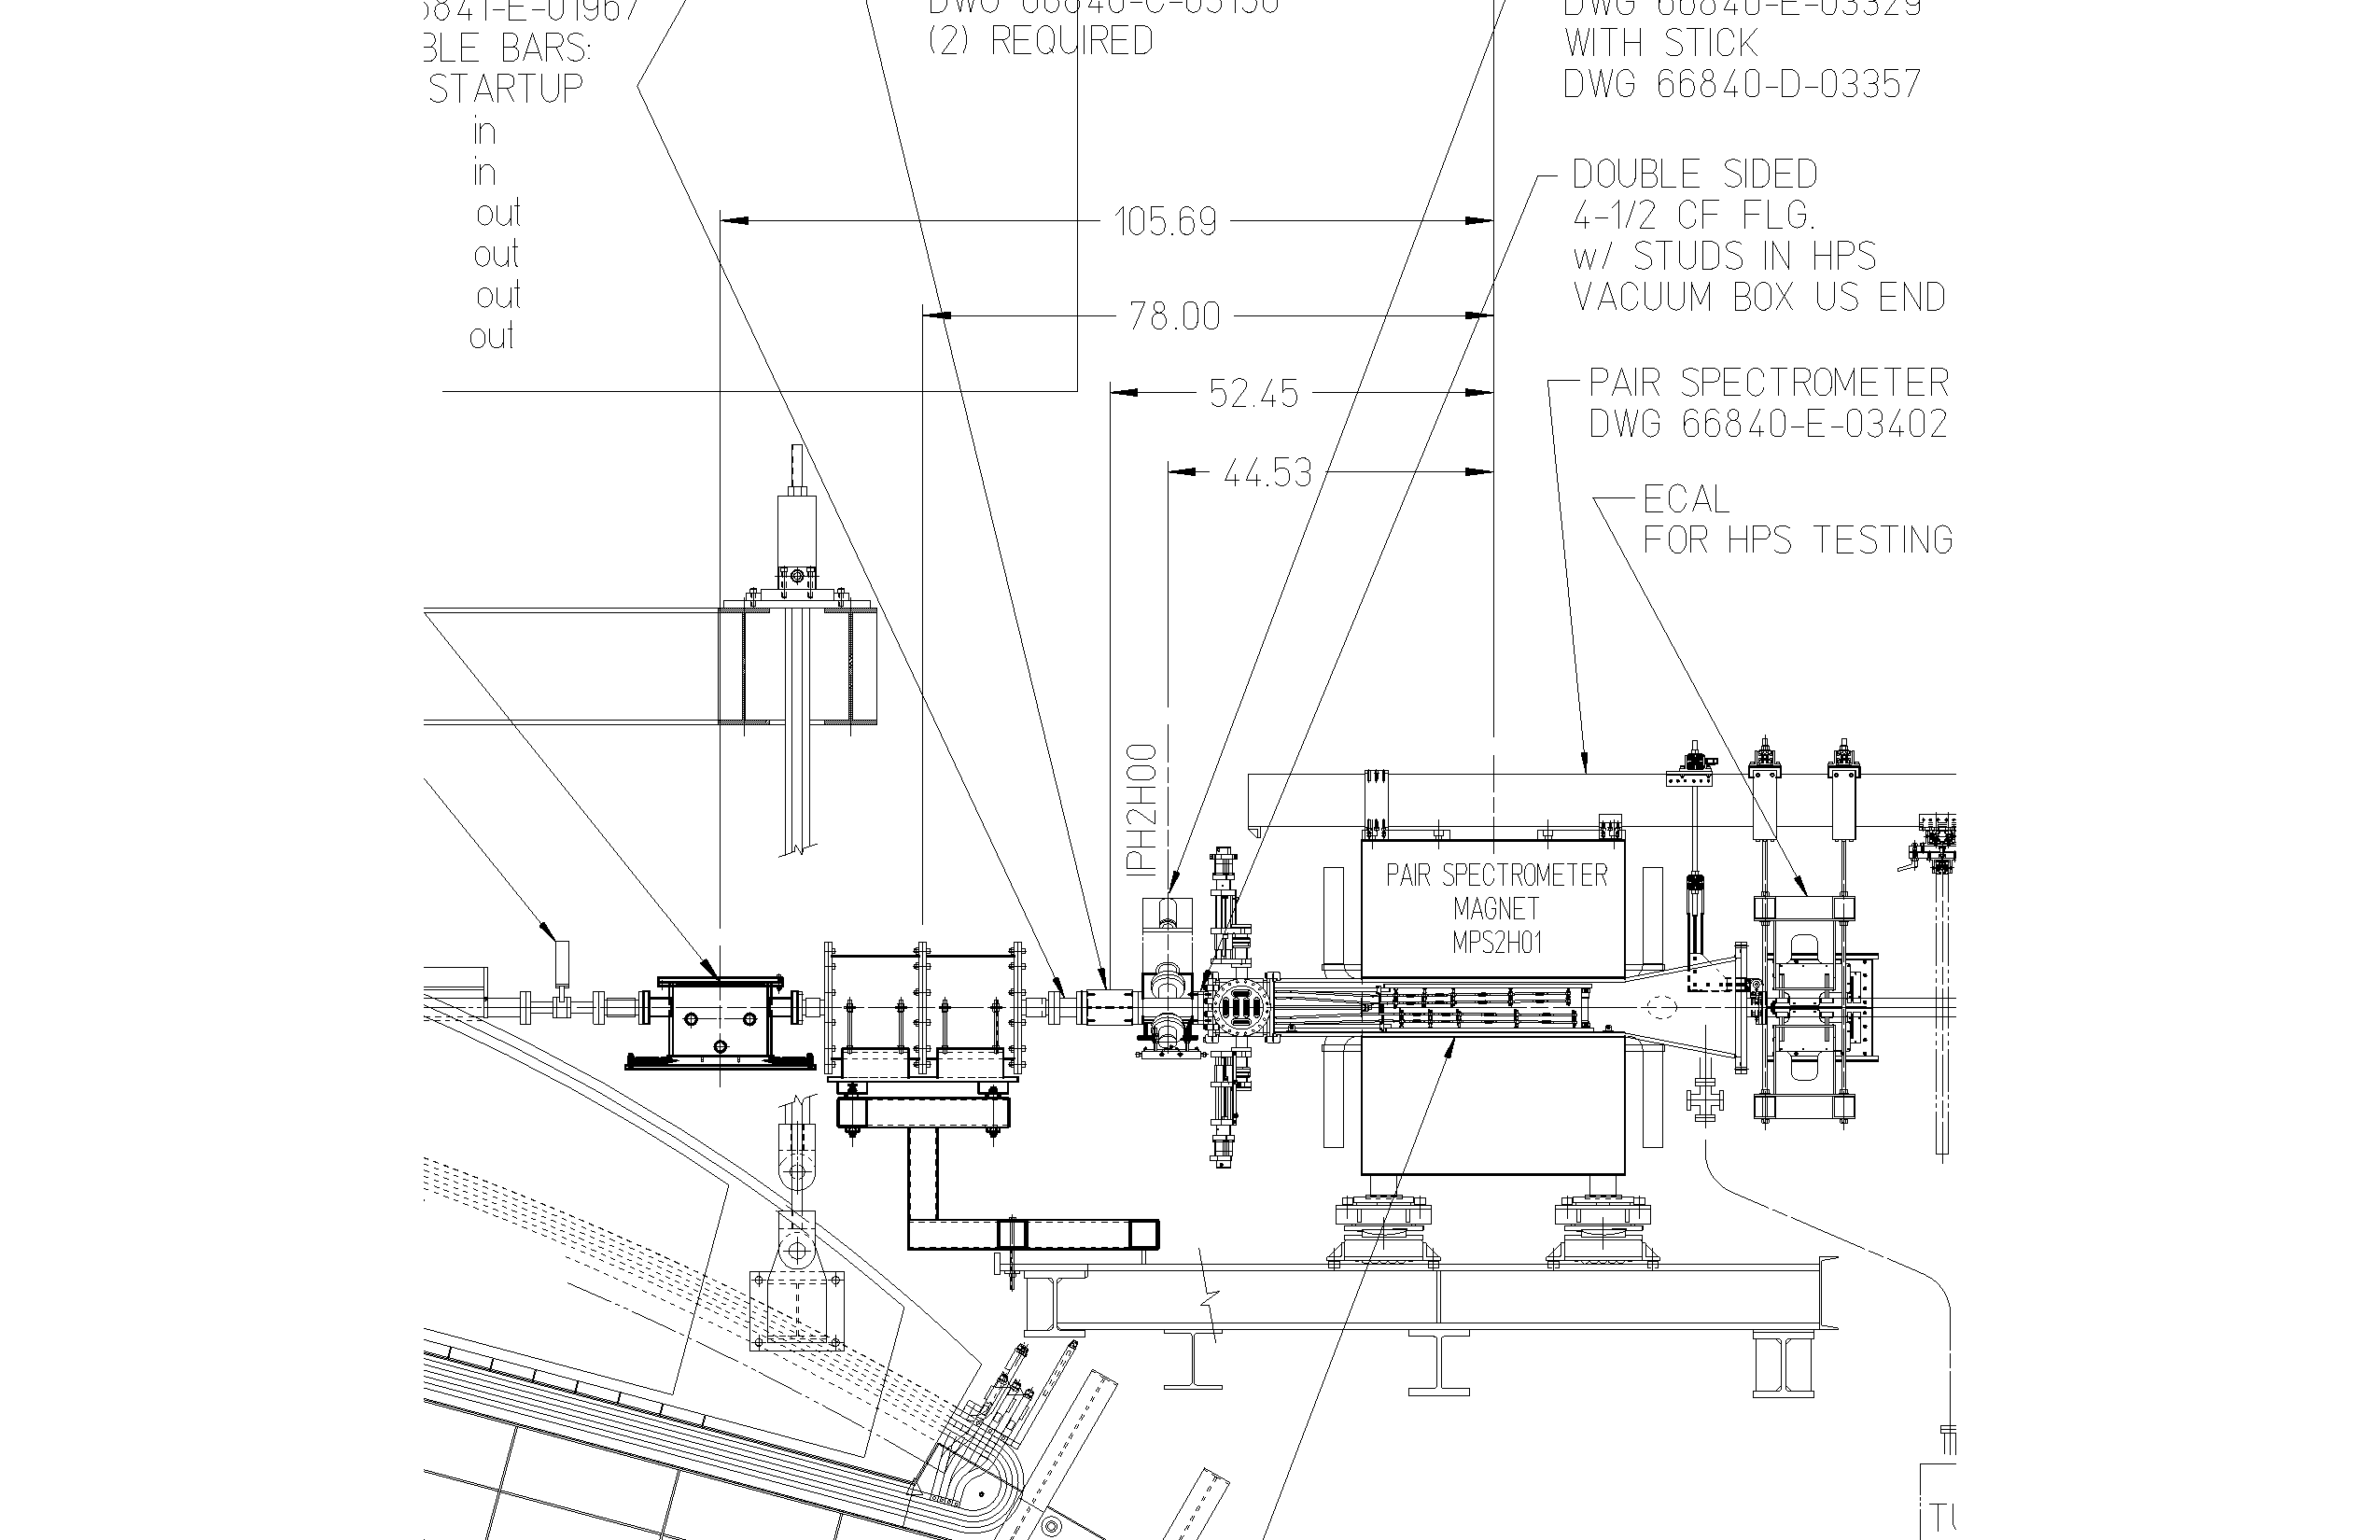
\includegraphics[width=\textwidth]{test2012/HPS_dimensions}
\caption{\small{Layout of the HPS parasitic run.} }
\label{fig:hpstest_layout}
\end{figure}

For the portion of the dedicated HPS run the photon beam was generated in the interaction of the $5.5$ GeV electrons with a gold radiator of $10^{-4}$ r.l., located $\approx 8$ meters upstream of the PS pair converter. After collimation ($D=6.4$ mm), the photon beam passes through the pair converter and through the HPS system. Data were taken on different converters (empty, $1.8\times 10^{-3}$ r.l., $4.5\times 10^{-3}$ r.l., and $1.6\times 10^{-2}$ r.l.). These measurements were repeated for reverse field setting of the pair spectrometer dipole.


\subsubsection{Test Run SVT}

The silicon tracking and vertexing detector for HPS Test, or SVT, operates in an existing vacuum chamber inside the pair spectrometer analyzing magnet in Hall B at JLab.  The design principles of the SVT are described in further detail in the HPS Test Run Proposal  \cite{HPS_tPROP}. There are five measurement stations, or ``layers,'' placed immediately downstream of the target. Each layer comprises a pair of closely-spaced planes and each plane is responsible for measuring a single coordinate, or ``view.'' Introduction of a stereo angle between the two planes of each layer provides three-dimensional tracking and vertexing throughout the acceptance of the detector with one redundant layer. 

In order to accommodate the dead zone, the SVT is built in two halves that are mirror reflections of one another about the plane of the nominal electron beam.  Each half consists of five double-sided modules mounted on a support plate that provides services to the modules and allows them to be moved as a group relative to the dead zone. Each module places a pair of silicon microstrip sensors back-to-back at a specified stereo angle with independent cooling and support.

100 milliradian stereo is used in the first three layers to provide higher-resolution 3-d space points for vertexing. The 50 milliradian stereo of the last two layers breaks the tracking degeneracy of having five identical layers and minimizes fakes from ghost hits, improving pattern recognition while still providing sufficient pointing resolution into Layer 3 for robust hit association in the denser environment there. These stereo angles are the same as those proposed in Section \ref{sec:svtt} for the new SVT. The details of the five layers are shown in Table \ref{tab:trk} and a solid model of the detector layout is shown in Figure \ref{fig:tracker_model}.  Figure \ref{fig:tracker_halves} shows a photograph of both completed detector halves prior to final assembly.  Altogether, this layout comprises 20 sensors and hybrids and 100 APV25 chips for a total of 12780 readout channels. 

\begin{table}[h]
\begin{center}
\begin{tabular}{lccccc}   
\hline \hline 
    Layer & 1 & 2 & 3 & 4 & 5 \\      
\hline
    nominal $z$, from target (cm)  & 10 & 20 & 30 & 50 & 70  \\ 
    Stereo Angle (mrad)  & 100 & 100 & 100 & 50 & 50 \\ 
    Bend plane resolution ($\mu m$)  & $\approx$6 & $\approx$6 & $\approx$6 & $\approx$120 & $\approx$120  \\ 
    Non-bend plane Resolution ($\mu m$)  & $\approx$6 & $\approx$6 & $\approx$6 & $\approx$6 & $\approx$6  \\ 
    \# sensors  & 4 & 4 & 4 & 4 & 4  \\ 
    Nominal dead zone  & $\pm1.5$  & $\pm3.0$  & $\pm4.5$  & $\pm7.5$  & $\pm10.5$  \\ 
    Power consumption & 6.9 & 6.9 & 6.9 & 6.9 & 6.9 \\
\hline \hline
\end{tabular}
\caption[]{Layout of the HPS SVT. }
\label{tab:trk} 
\end{center}
\end{table}

\begin{figure}[ht]
    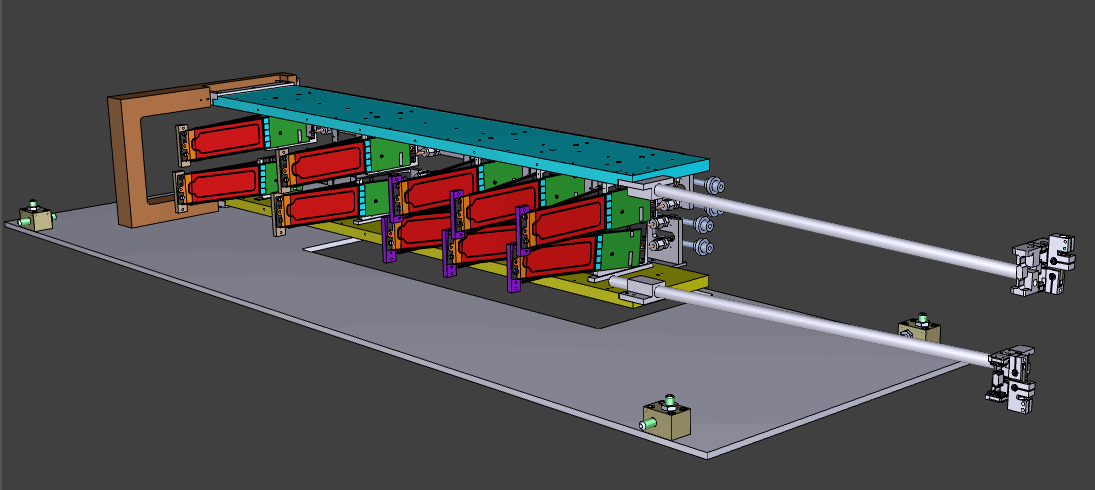
\includegraphics[width=\textwidth]{test2012/HPS_nocables_nowires}
\caption{\small{A partial rendering of the HPS Test SVT solid model showing the modules of the upper and lower half-detectors on their support plates, the hinged C-support, the motion levers, the cooling manifolds on their strain relief plate and the baseplate with its adjusters.  The sensors are shown in red and the hybrids in green. The beam enters from the right.} }
\label{fig:tracker_model}
\end{figure}

\begin{figure}[ht]
    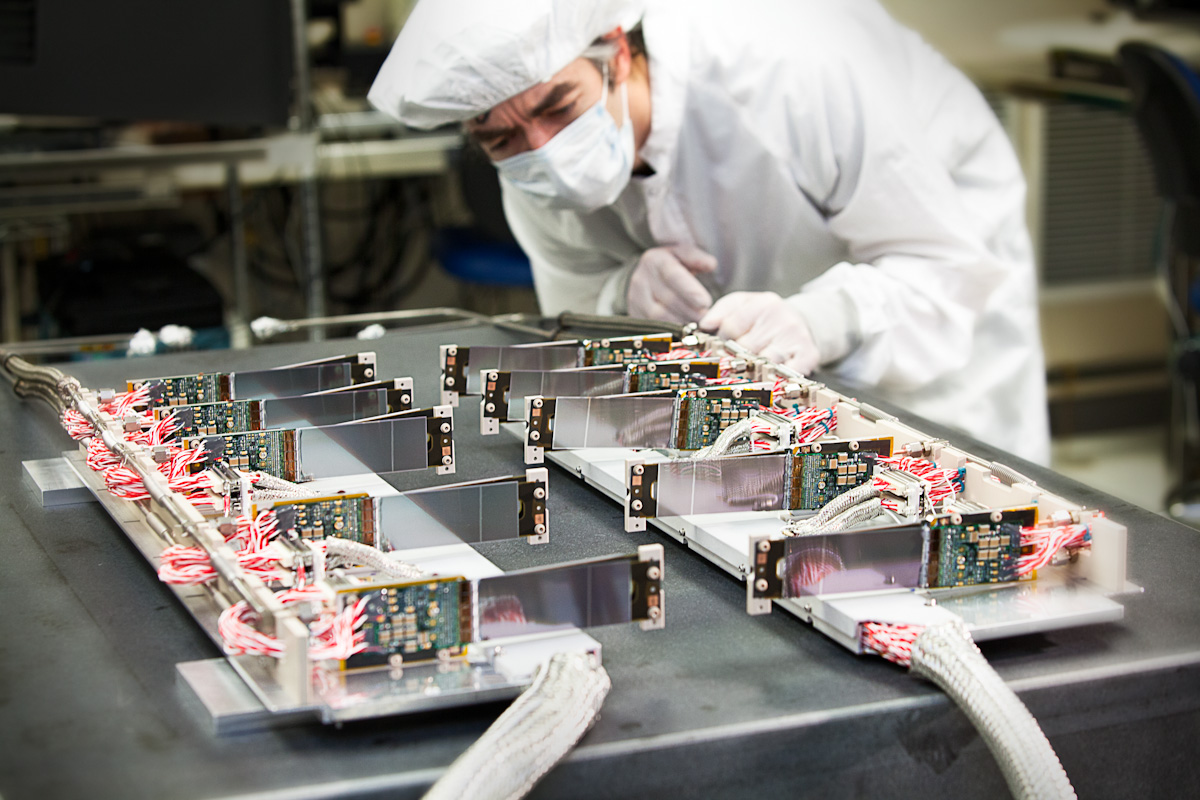
\includegraphics[width=\textwidth]{test2012/2012-101-PHOTON-DETECTOR-001.jpg}
\caption{\small{Both halves of the HPS Test SVT fully assembled at SLAC.} }
\label{fig:tracker_halves}
\end{figure}

Power is provided to each hybrid using CAEN power supplies provided by Fermilab. Three low voltages are supplied for the APV25 and one high voltage to reverse bias the sensor. The supplies that provide sensor bias are capable of 500V operation and can be used to test operation at high voltage in close proximity to an electron beam. The total power consumption of each hybrid during normal operation is about 2 W, which is removed with the cooling system. Care was exercised in selecting power and data cables, to ensure vacuum compatibility and sufficient radiation hardness. The teflon-coated twisted pair copper wires selected are rated for 400kRad, well above the expected exposure of 20kRad/week. A special purpose junction box interfaces the CAEN power supply output channels to the SVT hybrids. Control of the supplies is provided via an EPICS graphical user interface, which allows monitoring of the detector and interlock protection as well.

The linear shifts that define the opening of the SVT are controlled by a pair of stepper motors located in low field regions at the ends of the analyzing magnet.  For photon running, these are locked in the open position, but for electron running they will be connected and controlled through EPICS so that the distance between the beam and the sensors can be adjusted to balance detector occupancies and acceptance.


\subsubsection{Test run ECal}

The electromagnetic calorimeter (ECal) for HPS, as described in Section \ref{sec:ecal}, was built and tested in the test run.
The only differences between the test run ECal and what is proposed here for HPS are in the position and the vacuum chamber.

The vacuum chamber between the two ECal modules was not used for the photon test run, instead 2'' beam pipe was used to transport photon beam from the pair spectrometer vacuum chamber to the HDIce target.  
The ECal was mounted downstream of the analyzing dipole magnet at the distance of $\sim 148$ cm from the upstream edge of the magnet. The two ECal modules are positioned just above and below the beam pipe such that the edge of the crystal closest to the beam is $3.7$ cm from it. 

{\color{red} check beam pipe diameter: 2 inch, 3 inch or 2.5 inch?}
%It centered relative to the beam that passes in between two parts of ECal through $3$ inch beam pipe.

\begin{figure*}[t]
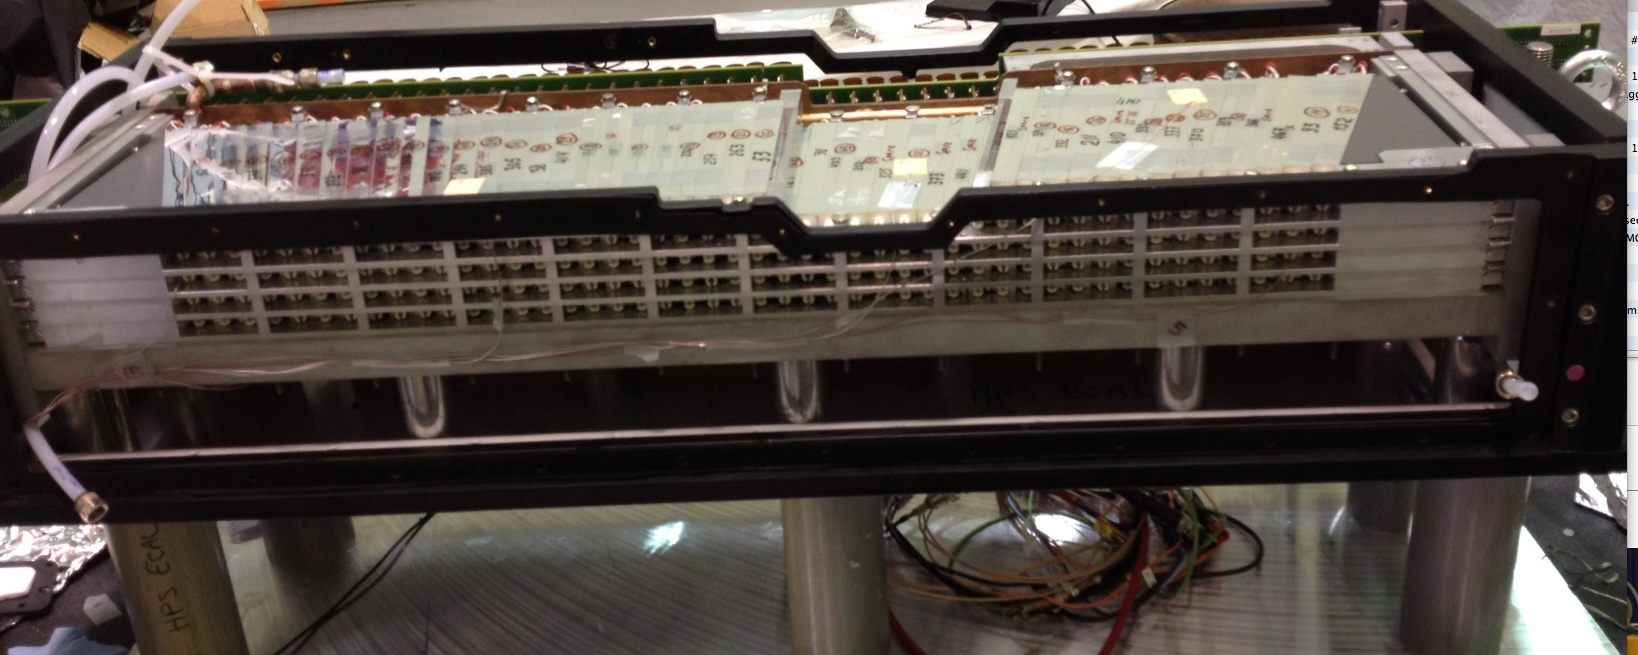
\includegraphics[ scale=0.25]{test2012/ecal_assembly.jpg}
\caption{\small{Assembly of the ECal bottom module.}}\label{fig:ecal_assembly}
\end{figure*}

%In order to maintain stable performance of the PbWO$_4$ calorimeter, the crystals and APDs are enclosed within a temperature stabilized environment, held constant at the level of $1~^o$F. The expected energy resolution of the system from operational experience with the IC is $\sigma_E/E \sim 4.5\% / \sqrt{E (GeV)}$. As in the IC, PbWO$_4$ modules are connected to a motherboard that provides power to and transmits signals from individual APDs and pre-amplifier boards. Crystals inside the box are supported by aluminum frames, Figure \ref{fig:ecal_assembly}.

For this run the ECal made use of the existing low and high voltage systems from the CLAS/IC, as well as signal cables and splitters. Connectors on the existing signal cables have been rearranged to accommodate the new layout of the channels. 

Figure \ref{fig:ecal_assembly} shows assembly of the bottom half of the ECal. 
In Figure \ref{fig:ecal_mounted} the ECal is shown in its installed position for the parasitic run with photon beam.
 

\begin{figure*}[t]
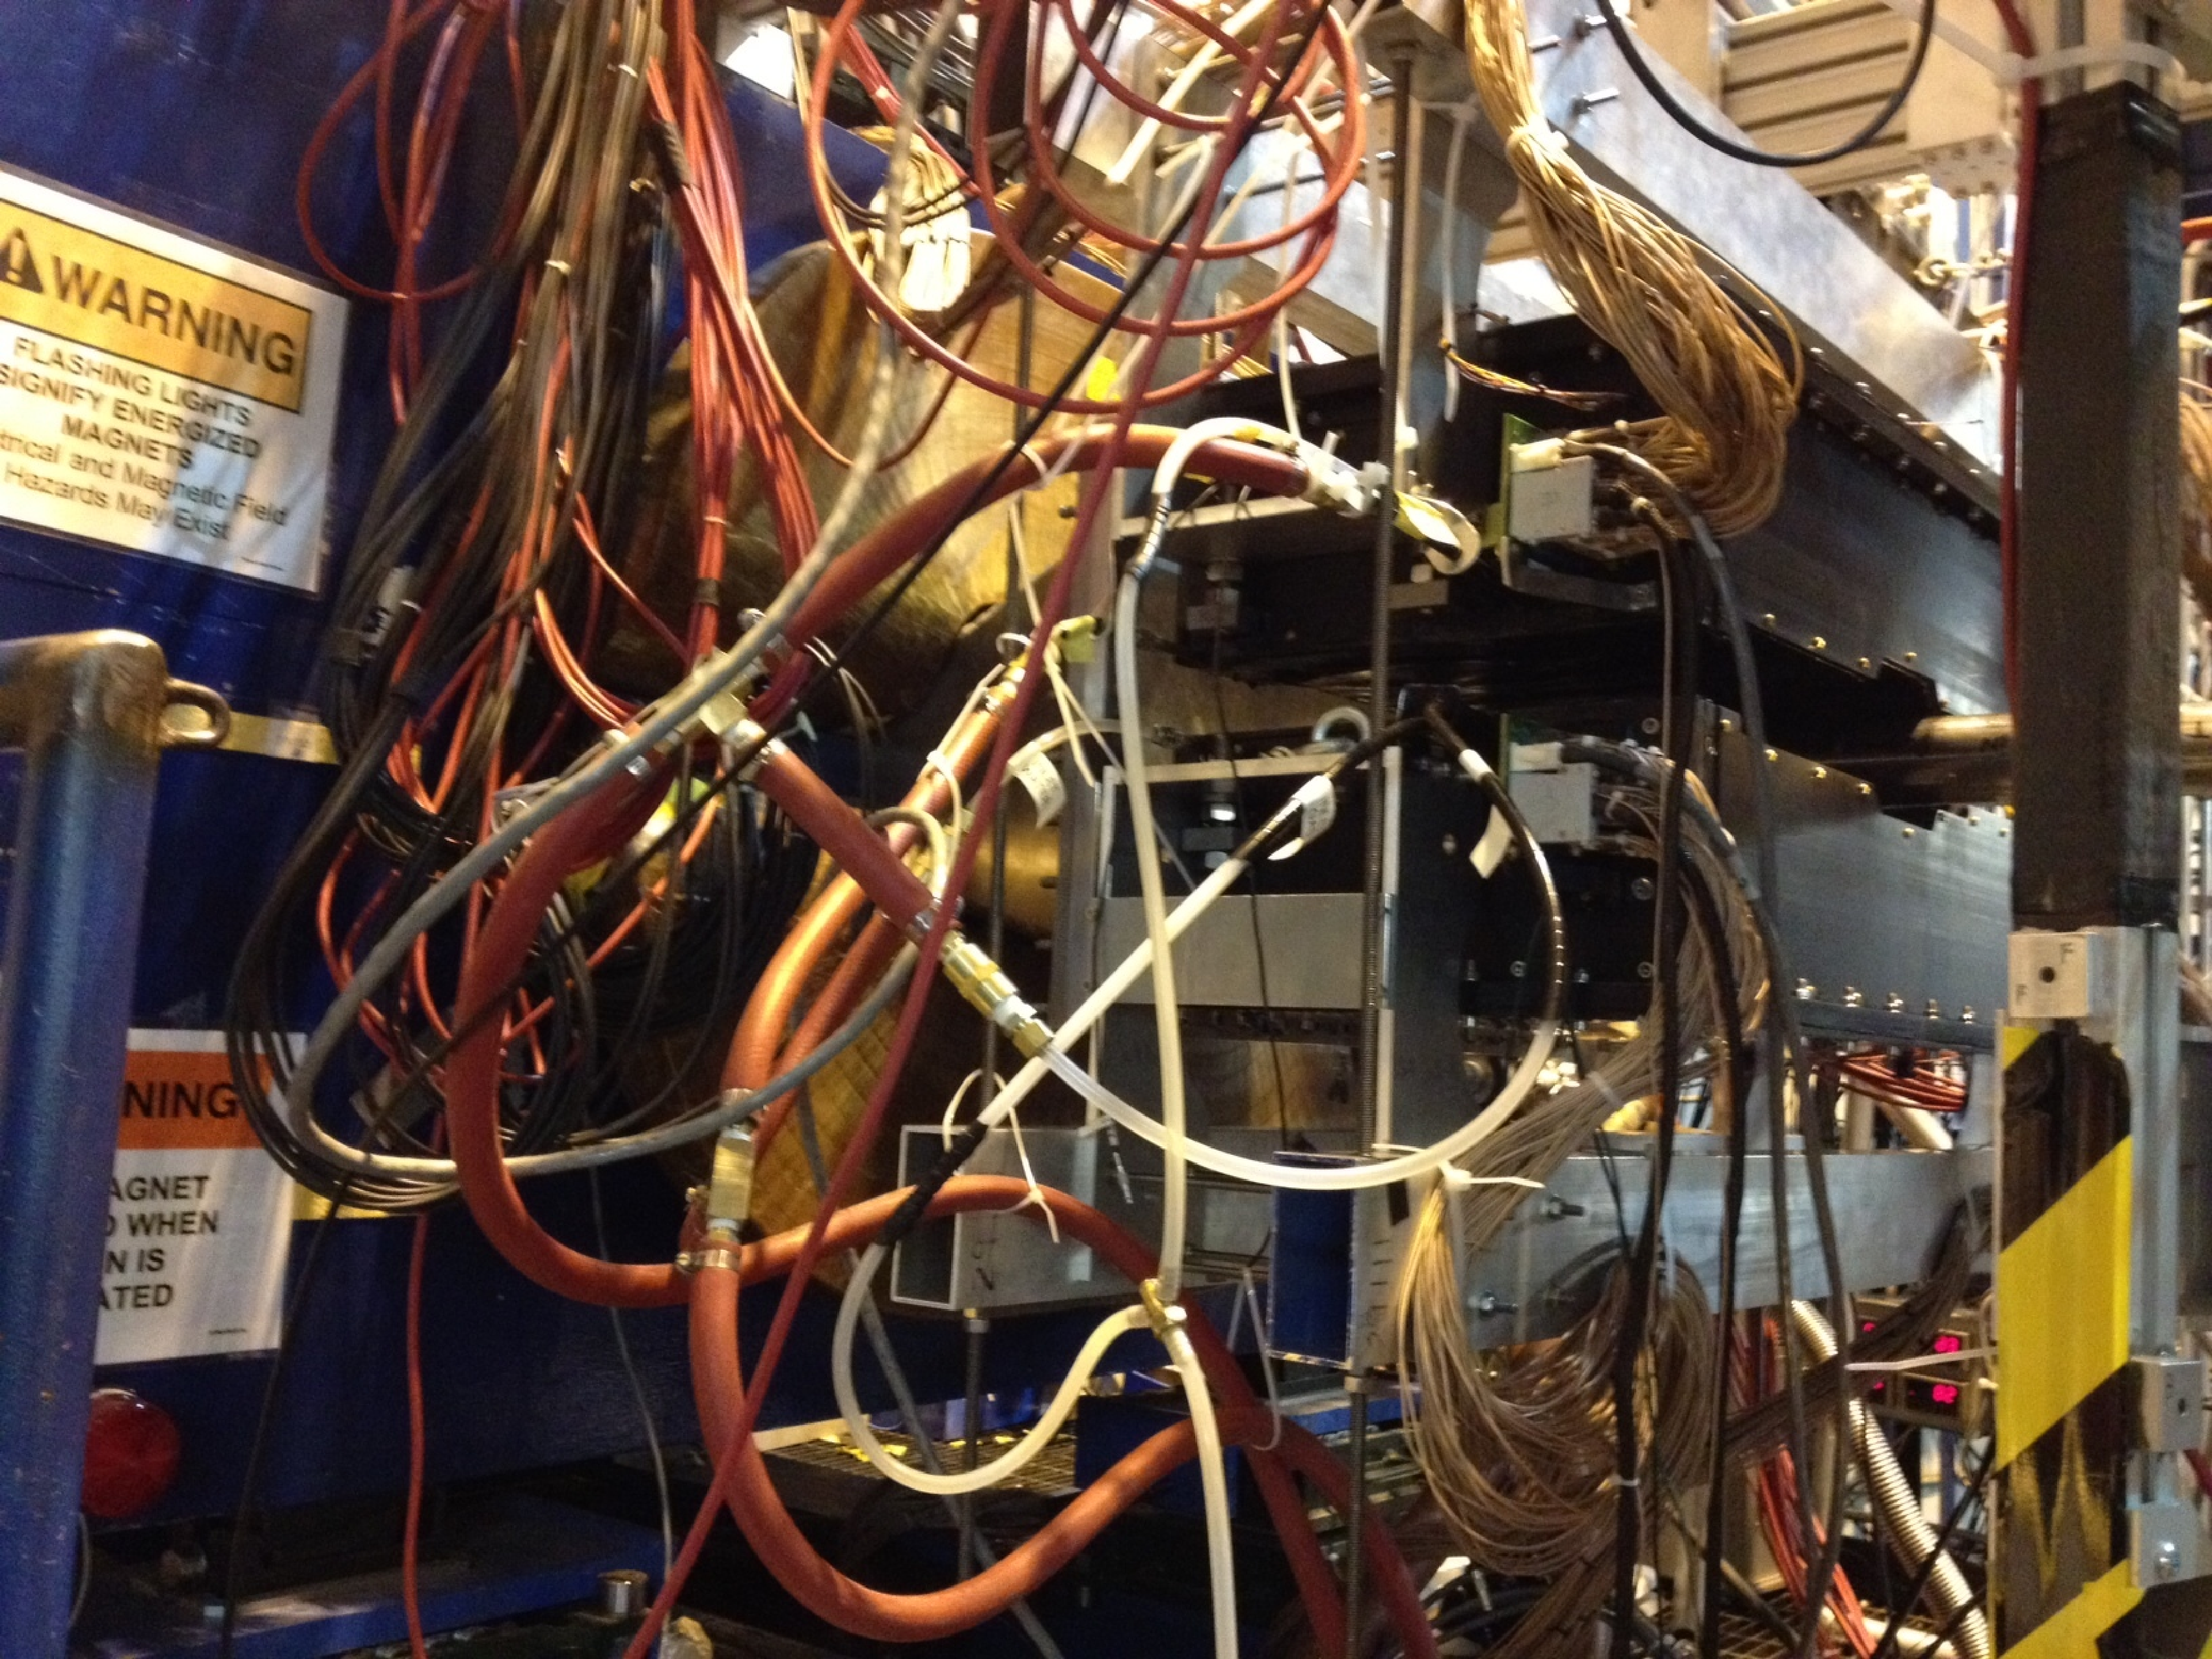
\includegraphics[ scale=0.25]{test2012/ecal_mounted}
\caption{\small{ECal mounted downstream of the Hall-B pair spectrometer for the parasitic run with photon beams. Hoses for the cooling system, and the power and signal cables for beam-right side of both modules are visible.}}\label{fig:ecal_mounted}
\end{figure*}



\subsubsection{Test Run Data Acquisition}
\label{sec:testrun_daq}
%This section describes the overall design of the DAQ system used in the test run. 
%Considering the similarity to the 
%system proposed for HPS only a brief description is given here, with an emphasis on the differences. 
%Results, milestones and experiences attained from operating the DAQ in the test run is also presented. 

%The DAQ system for the HPS test run handles the data and trigger distribution for the ECal and SVT. 

The data acquisition system (DAQ) for the HPS Test run was a somewhat simplified version of the DAQ proposed for HPS in Sec.~\ref{sec:daq}. In addition to simpler trigger logic, the primary difference for the ECal is different signal processing for the trigger which results in slightly worse single-crystal energy resolution and no possibility to calibrate individual crystal gains at the trigger level.  For the SVT, the smaller
number of channels eliminated the need for optical conversion and aggregation of data and detector power inside the vacuum chamber.
Finally, most data links had 1 Gbit bandwidth, sufficient for the purposes of the test run.

In other respects, the HPS Test run DAQ was essentially identical to that proposed for HPS and used to verify the overall technical approach of the system. The ECal provides data to the FADC-based Level~1
trigger system. Accepted events are read out from the ECal and SVT DAQ and processed by an event builder before output to disk.
For the ECal, the Readout Crate Controllers (ROCs) were the same as those proposed for HPS and are installed in VME, VME64X and VXS 
crates running mvme6100 controllers, with prpmc880 or pmc280 co-processor modules. For simplicity, a hybrid approach was 
used for the SVT DAQ in the test run where the ROC ran on a external PC connected to the ATCA crate. Similar to that proposed for HPS, a 
Foundry Router was used as the backbone of the DAQ system, providing 1~Gbit and 10~Gbit connections between components 
and to the JLAB Computer Center. The Event Builder, Event Recorder, and other critical DAQ components ran on 4-CPU Opteron-based servers, 
which was sufficient for the test run. The RAID5 storage system had 100~MB/s capability, sufficient to handle the anticipated data rates for electron running.


%The DAQ system built for the HPS test run was a proof of principle for that proposed for HPS, described in 
%Sec.~\ref{sec:daq}. Consequently, the architecture of the systems are very similar. The main differences 
%for the ECal and trigger, in addition to the simpler trigger logic, is a different trigger and readout data 
%path. This resulted in a lower crystal energy resolution and no possibility of crystal gain calibration at the 
%trigger level. The smaller SVT relaxed the need for optical conversion and for signal and power aggregation 
%inside the vacuum chamber. 
%Most of the data links were 1~Gbit bandwidth, large enough given the data rates expected in the test run.
%
%
%
%The two front-end electronics systems for the ECal and SVT are essentially unchanged compared to the HPS 
%DAQ system. The ECal provides 
%input to the Level~1 trigger system after which an accepted event is acquired from the two sub-systems 
%and are processed. The Readout Crate Controllers (ROCs)
% described for HPS are unchanged and installed in every VME, VME64X, VXS crates running 
% mvme6100 controllers with a prpmc880 or pmc280 co-processor modules. A hybrid approach was 
% used for the SVT DAQ in the test run where the ROC ran on a external PC connected to the ATCA crate. 
% Similar to HPS, a Foundry Router was used as the backbone of the DAQ system, providing 1~Gbit and 
% 10~Gbit connections between components and to the JLAB Computer Center. The Event Builder, Event 
% Recorder, and other critical DAQ components ran on 4-CPU Opteron-based servers, which was sufficient 
% for the test run. The RAID5 test run storage system had a 100~MB/s capability to handle the data rates 
% expected for the test run as described below.

%\subsubsection{SVT DAQ}

The SVT DAQ was designed to read out data continuously at 40~MHz from the SVT modules and transfer data 
to the JLab DAQ once a trigger signal is received. It is based on the same overall architecture as the system 
described in Sec.~\ref{sec:svt_daq}. Being only half the size of the HPS SVT, the largest difference is the provision for
individual power and data for each sensor and readout chip from the power supplies and DAQ outside of the vacuum chamber.
This simplification reduced development time and cost at the expense of a large number of connections and vacuum feedthroughs.
With a total of 20 silicon microstrip sensors, each one connected to an onboard hybrid readout 
card hosting five 128-channel APV25 ASICs (shown in Figure ~\ref{fig:hybrid_and_apv25_testrun}), 600 lines for power and data are required.
 \begin{figure*}[t]
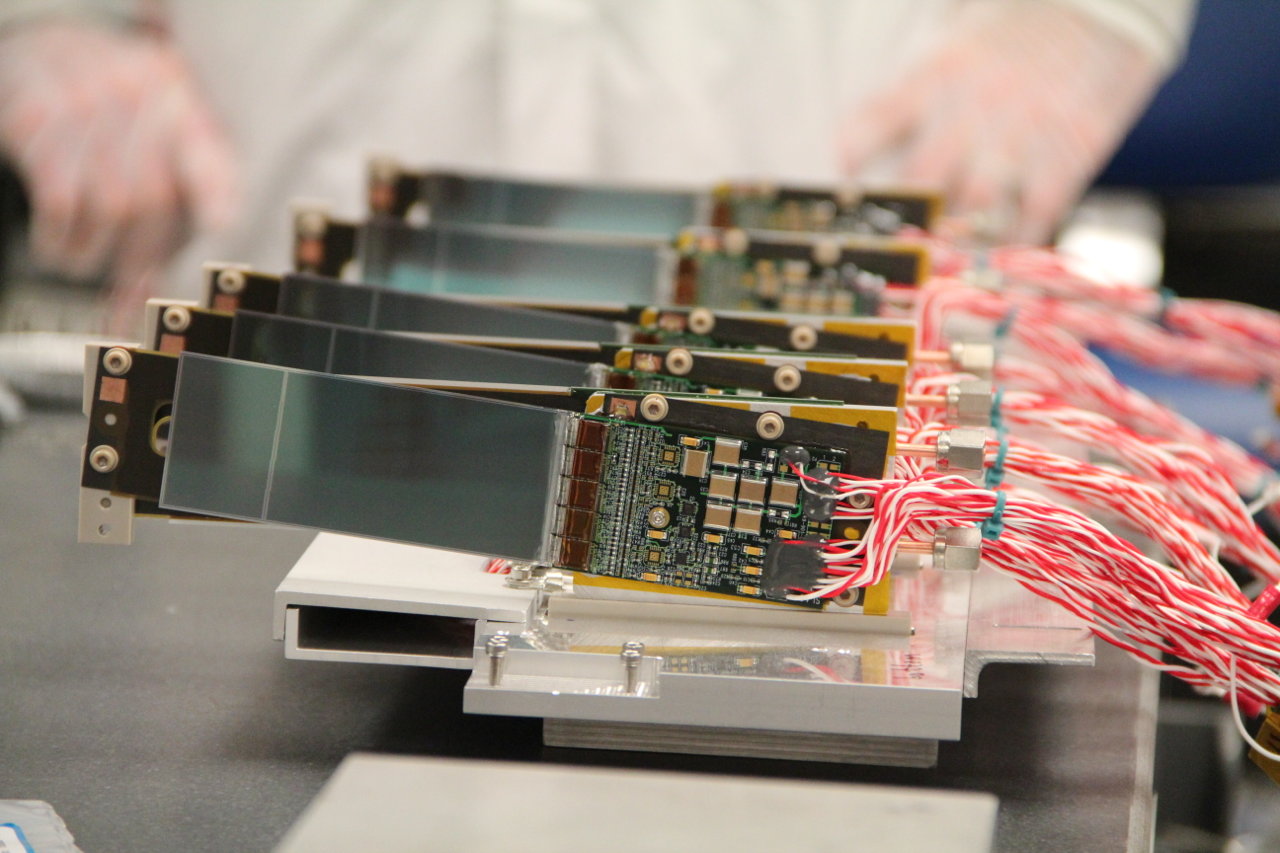
\includegraphics[ scale=0.3]{test2012/daq/svt_modules_on_sup_plate.png}
\caption{\small{View from upstream of one half of the SVT modules mounted on the support plate. Signal, 
power and control are soldered, and potted, to pads at one end while the five APV25 chips are wirebonded 
to the silicon sensor at the other.}}
\label{fig:hybrid_and_apv25_testrun}
\end{figure*}
Without optical conversion inside the chamber as proposed for HPS, analog signals from the APV25 chips are 
carried directly to the ATCA crate located outside the vacuum chamber via multi-twisted-pair cable. 
The amplification and digitization is carried out on a Rear Transition Module (RTM) board designed specifically for the HPS test run. 
On the RTM, a pre-amplifier converts the APV25 differential current output to a voltage output 
scaled to the sensitive range of a 14-bit ADC. The RTM is organized into four sections with each section 
supporting 3 hybrids (15 channels). The ADC is operated at the system clock of 41.667~MHz. 
%The RTM also includes a 4-channel Fiber Optic module and supporting logic which can be used to interface to the JLAB trigger supervisor card.
The ATCA main board, the Cluster on Board (COB), is similar to the one described for the HPS DAQ 
with the important exception that one of the Data Processing Modules (DPMs) functions as the trigger 
interface and there is no Reconfigurable Cluster Element (RCE) module. Instead, the DPMs that package and send the data from the hybrids to 
an external PC through a 1~Gbit/s ethernet connection serve the same purpose as the 
RCE module in the HPS DAQ. Figure~\ref{fig:svtdaq} shows an overall layout of 
the SVT DAQ system used for the test run (compare to Fig.~\ref{fig:svt_daq_overview}).
 \begin{figure}[t]
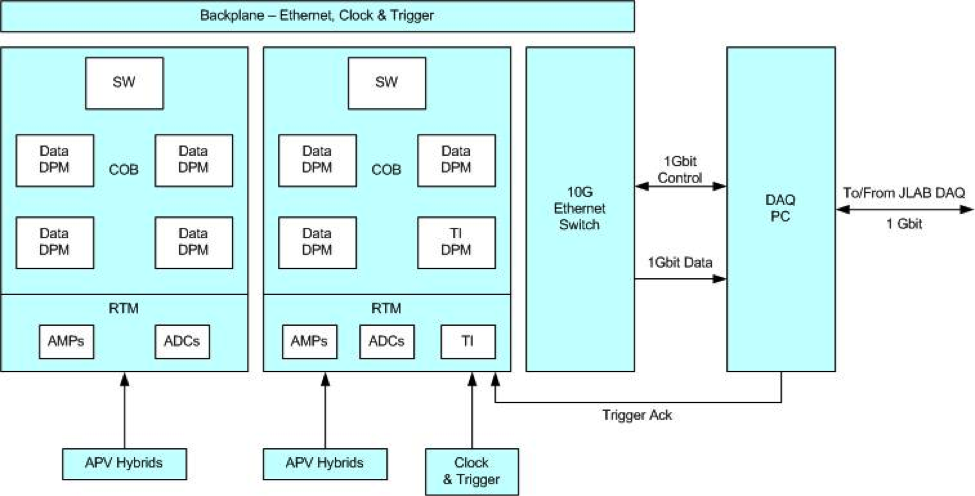
\includegraphics[scale=0.9]{test2012/daq/svt_daq_diagram.png}
\caption{\small{Schematic of the SVT DAQ used for the test run. Note that the hybrids are connected directly 
to the RTM and that an external DAQ PC is used for control and transfer of data to the JLab DAQ.}}
\label{fig:svtdaq}
\end{figure}
The ATCA crate hosts two COB cards, one supporting four data processing DPMs and the other supporting three data processing DPMs and one trigger DPM for a capacity of 21 hybrids, one more than required. 
The test run RTM and COB boards are shown in Fig.~\ref{fig:rtm_testrun}. 
\begin{figure*}[t]
\includegraphics[ scale=0.25]{test2012/daq/rtm.png}
\includegraphics[ scale=0.4]{test2012/daq/svt_daq_module_noted.png}
\caption{\small{Picture of a RTM (top) and COB board (bottom) used in the HPS test run 2012.}}
\label{fig:rtm_testrun}
\end{figure*}
The external PC supports three network interfaces, two standard 1~Gbit/s Ethernet and one custom low latency 
data reception card. The first Ethernet interface is used for slow control and monitoring of the eight 
DPM modules. The second Ethernet interface serves as the interface to the JLAB data acquisition system. The
low latency network interface is used to receive data from the SVT ATCA crate and supports a low latency, 
reliable, TTL trigger acknowledge interface to the trigger DPM. This PC hosts the SVT control and monitoring 
software as well as the ROC application described above.



Signals from each module are sent to a signal splitter. One of the outputs of the splitter is fed to a discriminator that also has an internal scaler, and then to a TDC channel. The other output is sent to the Jefferson Lab FADC250 VXS module, Figure \ref{fig:fadc}. Two FADC crates are required for the  two modules. The trigger from the ECal is based on FADC information and includes a cluster finding algorithm using FPGA modules. It is described in Section \ref{trigger}. With the FADCs, the energy of clusters will be determined at the crate trigger level and will be used in making the trigger decision.

\begin{figure}[t]
\includegraphics[scale=0.5]{test2012/daq/FADC250_Photo_001.jpg}
\caption{\small{FADC250 VXS module.}}\label{fig:fadc}
\end{figure}







\subsubsection{Test Run Trigger System}
\label{sec:testrun_trigger}
The trigger system used in the test run is described in the HPS status update to PAC39 \cite{HPS_PROP_UPD} in full detail; only the chief differences will be described here. 
It is generally similar to that described in Section~\ref{sec:triggerdaq}; the same hardware (FADC, CTP, and SSP) was used.

The key differences were in the FADC integration algorithm, the energy resolution reported by the FADC to the CTP, and the SSP trigger decision algorithm.

In the test run, the FADC used a time-over-threshold algorithm to integrate hit energy for use in trigger decision, where only samples above threshold were summed.
This algorithm is shown in Figure~\ref{fig:trigsamples}.

\begin{figure}[ht]
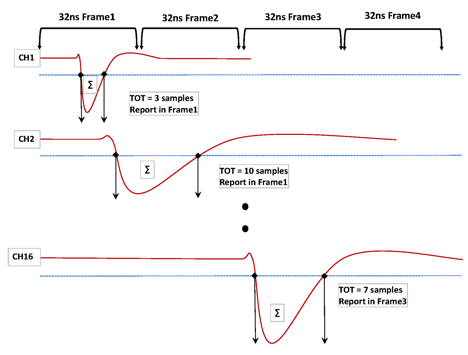
\includegraphics[scale=0.9]{test2012/trigger//trigger_pulse_samples}
\caption{\small{Example of input signals, and how they are integrated and digitized for the test run trigger.}}\label{fig:trigsamples}
\end{figure}

The FADC reported hits to the CTP in an 8-bit format consisting of a 5-bit channel sum and a 3-bit timestamp. This meant that the pulse integral had to be truncated to fit in 5 bits; consequently some energy resolution was lost. 
A block diagram of the FADC internal processing and reporting to the CTP is shown in Figure~\ref{fig:trigger_diagram}.  
\begin{figure}[ht]
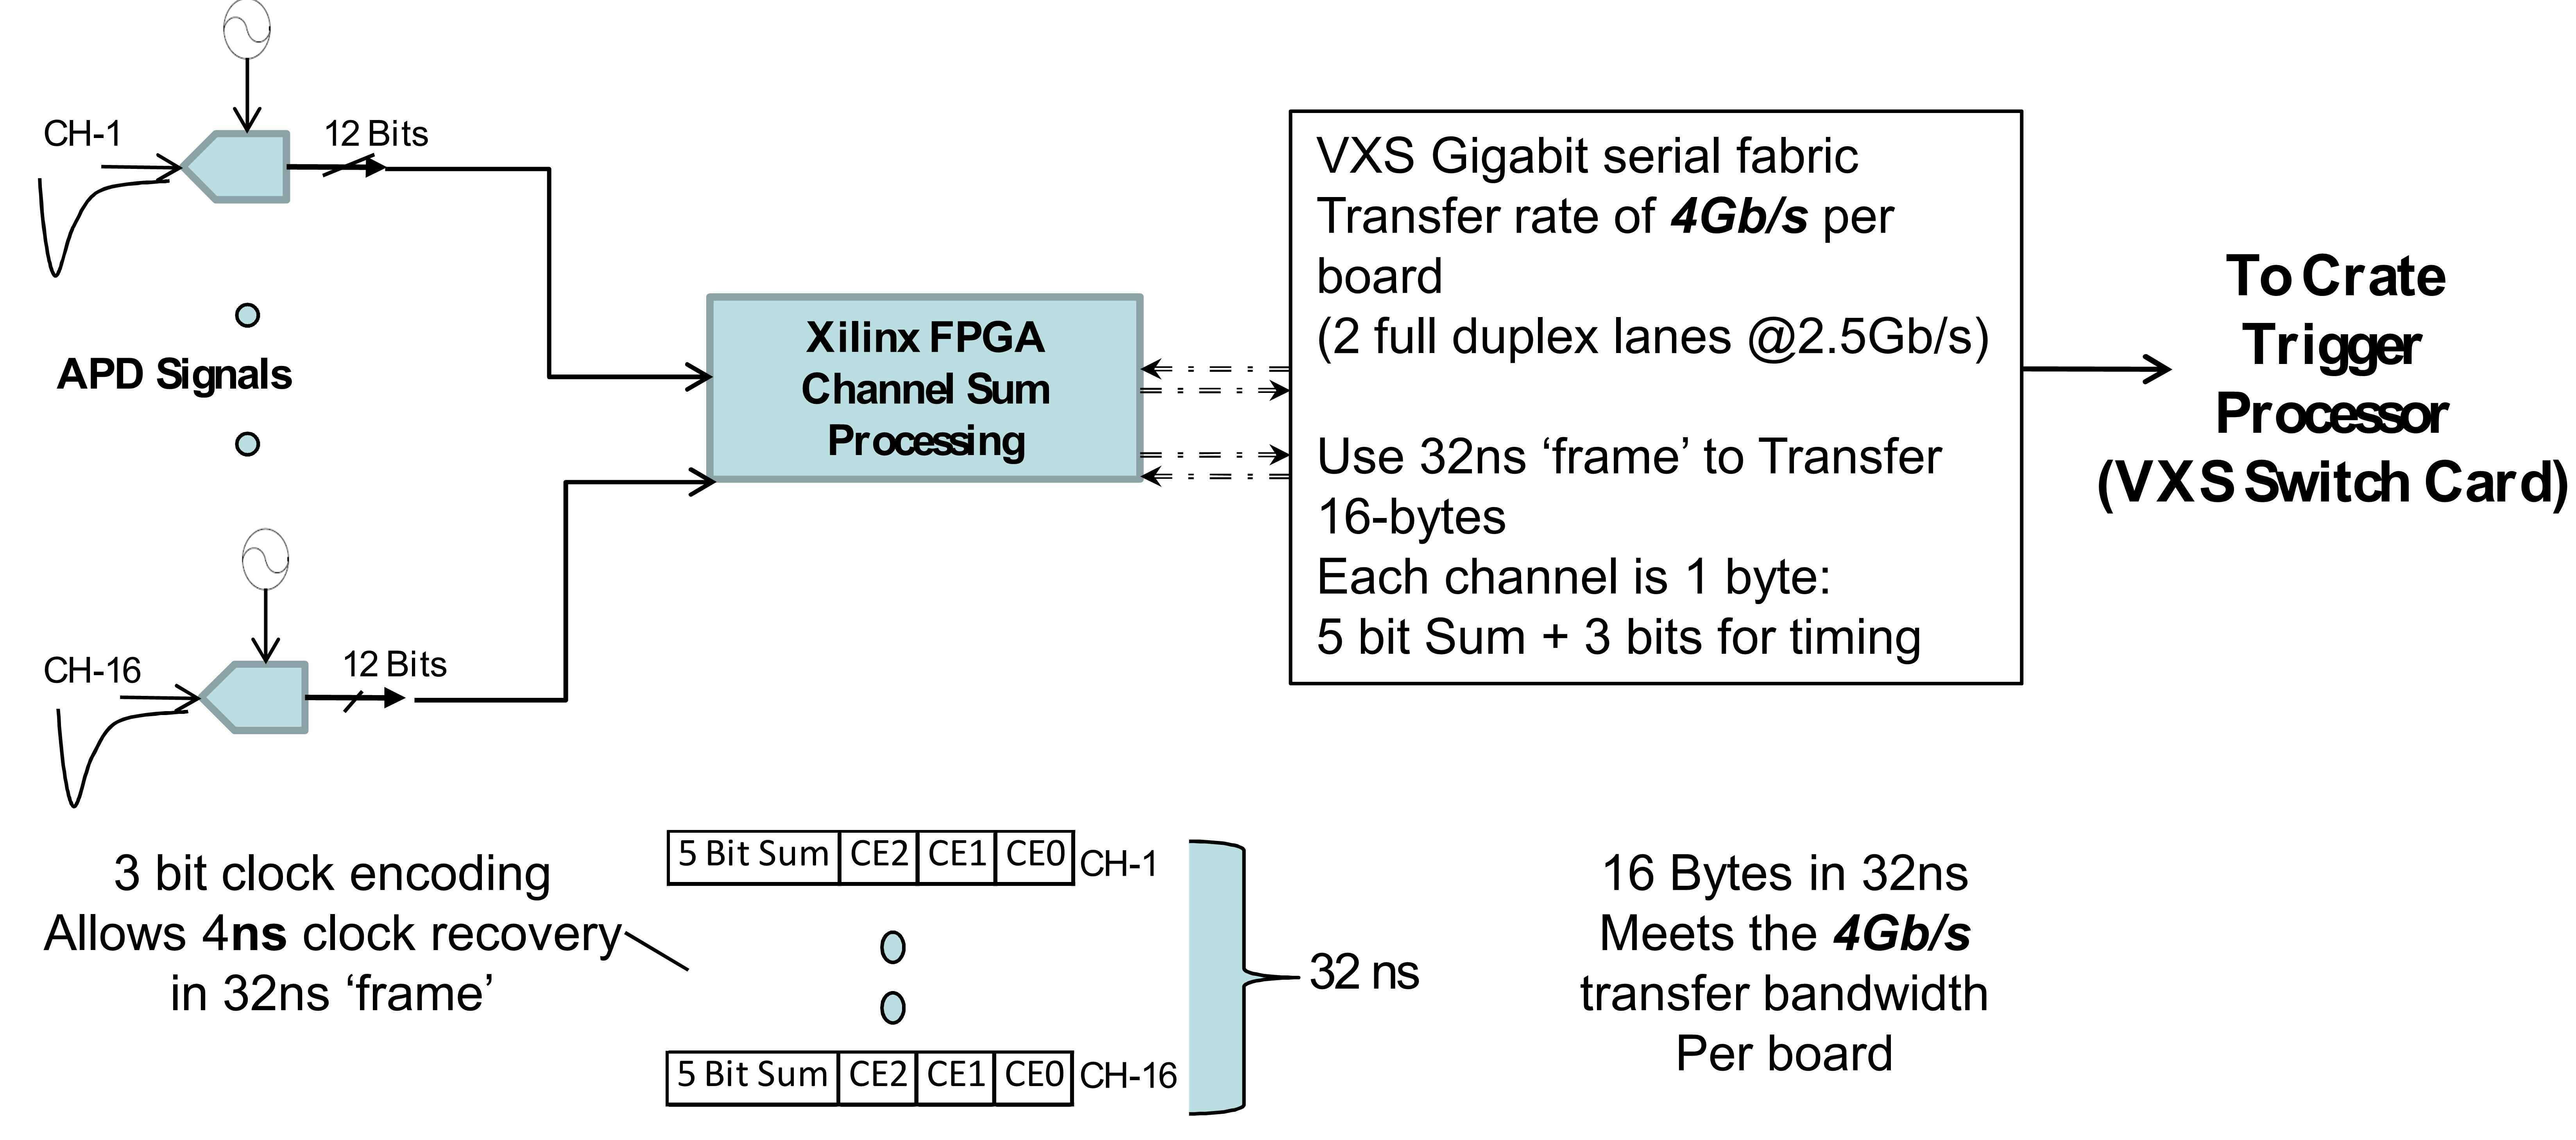
\includegraphics[scale=0.6]{test2012/trigger/HPSChanSum_001.jpg}
\caption{\small{Block diagram for the trigger system.}}
\label{fig:trigger_diagram}
\end{figure}
%The trigger is based solely on information from the FADC boards and utilizes gigabit bandwidth to transport all the 
%individual FADC channel sums (5-bits) and clock (3-bits) encoding bits. 
%The clock encoding bits report the 
%4~ns time period when the input signal crosses the programmable threshold within a 32~ns frame.  
%The reported 5-bit channel sum value is extracted from the 17-bit register that contains the integrated (sum) 
%signal value of the input channel. The channel integration occurs only if the input signal crosses the 
%programmable threshold level: if the input signal does not cross threshold for a given 32~ns frame, the channel data is reported as zero.
%The number of samples for a given channel integration cannot exceed the frame report latency time (128~ns or 32 samples) 
%and only those samples above threshold are included. The processing and digitization of input signals are illustrated in Fig.~\ref{fig:trigsamples}. 

%\begin{figure}[]
%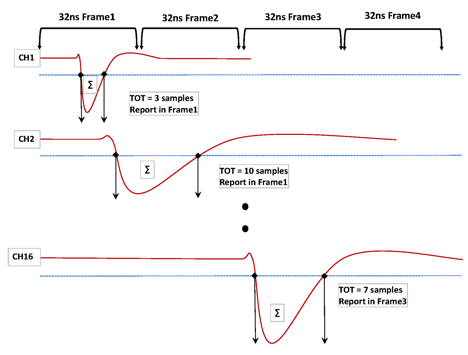
\includegraphics[scale=0.9]{test2012/trigger//trigger_pulse_samples}
%\caption{\small{Example of input signals, and how they are integrated and digitized for the test run trigger.}}\label{fig:trigsamples}
%\end{figure}
%The time within a 32~ns frame where the input signal crosses threshold determines in which frame the 
%integrated value is reported. Three clock encoding bits are used to time stamp the threshold crossing time to 
%a 4~ns window.  
%In the example, the pulse for channel~2 crosses multiple frames.  The point where the signal crosses threshold determines the frame where the integration value will be reported for the given channel.  The number of points that are above threshold will be limited to 32. 
%The trigger application only processes a single falling or rising edge per 32~ns frame. If multiple 
%pulses arrive on a single channel within a 32~ns frame, they are not resolved and thus create a pile-up 
%effect in the trigger system. However, multiple pulses per frame can be recovered from the readout data offline.

%Information from each FADC channel are reported to the Crate Trigger Processor (CTP) through gigabit 
%serial data streams. The sixteen serial data streams, one for each FADC board, were processed on a frame 
%by frame basis. The cluster finding algorithm (see Sec.~\ref{sec:triggerdaq}) produces a serial data 
%stream further processed by the Sub-System Processor (SSP), creating a readout trigger signal 
%distributed to the FADC and SVT ATCA crates to initiate event readout. The system was designed to withstand 
%a trigger accept rate higher than 50~kHz, above the limit set by the SVT DAQ.  

For the test run, the simplified trigger logic in the SSP was a simple threshold: the trigger was configured 
to fire on a single cluster with energy exceeding a given threshold. However, the full trigger described in 
Ref.~\cite{HPS_tPROP} was implemented and tested.







\subsection{Test Run Apparatus Performance} 
\label{sec:testrun_performance}
As noted above we only had the opportunity to tun the HPS test apparatus in the 
photon beam mode using the Hall-B pair 
spectrometer (PS) pair converter as a target, which is located $\sim 67$ cm from the first layer 
of the tracker. This section will report on a few selected preliminary results that aims to demonstrate 
our understanding of the main characteristics of the system. 

\subsubsection{SVT Performance}
\vspace{1cm}{\bf Calibration [Omar]}


Description of hit amplitude, baseline/gain calibration, noisy channels/chips, pulse shape cuts, occupancy. 

Plots: Response plot, gain, noisy channels vs run nr?, data/MC of noise hits,Data/MC plot of occupancy for some layers  

\vspace{1cm}{\bf Cluster reconstruction [Omar]}


Description of the cluster reconstruction.

Plots: mip distribution

\vspace{1cm}{\bf SVT timing [Sho]}

The time reconstruction algorithm described in \ref{sec:svtŧ} was used to fit a single hit to each SVT channel in each event.
Pileup was not considered due to the very low hit rate in the SVT.

As shown in Figure \ref{fig:apvfit}, values of fit $\chi^2$ fell in the distribution of $\chi^2$ for 4 degrees of freedom (6 points -- 2 fit parameters).

\begin{figure}[ht]
	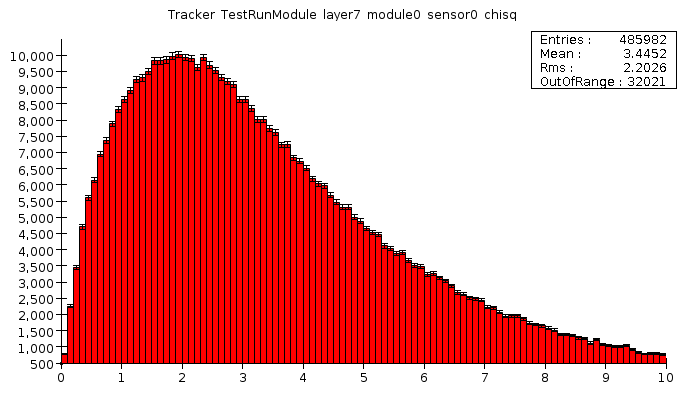
\includegraphics[width=\textwidth]{test2012/svtperformance/apvfit_chisq}
	\caption{\small{Histogram of $\chi^2$ values for pulse fits for all channels on a representative sensor. Peak at 2 is consistent with dof of 4, as expected.} }
	\label{fig:apvfit}
\end{figure}

After clustering these hits, the hit time for the cluster is computed as the amplitude-weighted average of the channel hit times. 



Since we have no measurement of the ``true'' hit time, we use the average of all cluster times in a track as the ``track time,'' and take the residual of the cluster time relative to that.
The track time, shown in Figure \ref{fig:tracktime}, has the expected amount of trigger jitter.
Different sensors have systematic offsets in hit time (up to a couple ns) due to time of flight and variations between readout chips. 
We correct these offsets so that the time residual is centered around 0 for each sensor. The RMS of the residual (from a Gaussian fit to the residual histogram, Figure \ref{fig:timeres}) is roughly 2.4 ns for each sensor.

\begin{figure}[ht]
	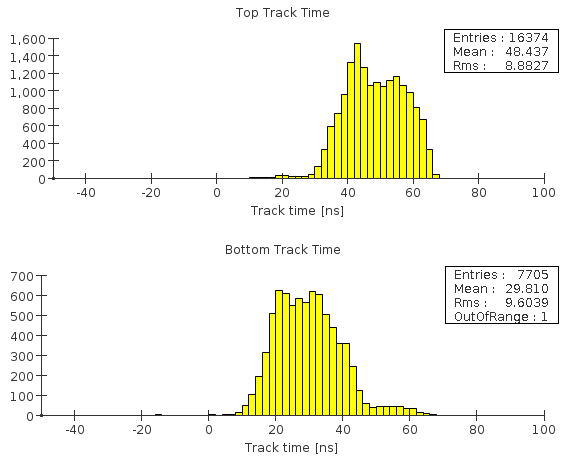
\includegraphics[width=\textwidth]{test2012/svtperformance/track_time}
	\caption{\small{Track time distribution, measured relative
	to the APV25 clock, for top and bottom tracks. The
width of the distribution is due to trigger jitter (24 ns
jitter in tracker readout clock, plus 16 ns jitter in the
trigger system). The shift between top and bottom
is due to a trigger time shift between the two halves
of the ECal.} }
	\label{fig:tracktime}
\end{figure}


Because the track time is calculated using the individual hit times, the hit time is positively correlated with the track time; thus the RMS of the residual is slightly smaller than the true time resolution.
The standard deviation of this residual for $n$-hit tracks where all hits have the same time resolution is reduced by a factor of $\sqrt{(n-1)/n}$; since most of our tracks have 8 clusters, the true time resolution is 2.6 ns. 

\begin{figure}[ht]
	\includegraphics[width=\textwidth]{test2012/svtperformance/timeres}
	\caption{\small{Histogram and Gaussian fit of residual of cluster times for a representative sensor, relative to the track time. Because the cluster times and track time have positive covariance, the true time resolution is slightly larger than the standard deviation shown here.} }
	\label{fig:timeres}
\end{figure}

%\begin{figure}[ht]
%	\includegraphics[width=\textwidth]{test2012/svtperformance/hit_dt}
%	\caption{\small{} }
%	\label{fig:hit_dt}
%\end{figure}

This is somewhat worse than the $\approx 2$ ns resolution expected, but we believe this discrepancy is due to our fit function. Our pulse shape fit assumes an ideal CR-RC pulse shape; since the actual pulse shape has a slower rise time, there is a systematic pull on the hit time when a hit comes immediately before the APV clock time. 
This is visible in Figure \ref{fig:timeres_2D} as a shift in the residual at certain values of track time.
Work is in progress to use the actual pulse shape in time reconstruction; this should improve time resolution.

\begin{figure}[ht]
	\includegraphics[width=\textwidth]{test2012/svtperformance/timeres_2D}
	\caption{\small{Plot of the time residual for a representative sensor vs. the track time. 
		The kinks in the horizontal band are caused by the fitter; without them the 1-D histogram in Figure \ref{fig:timeres} (the projection of this histogram) would be narrower.} }
	\label{fig:timeres_2D}
\end{figure}

\vspace{1cm}{\bf Tracking algorithms [Matt/Omar]}


Pattern recognition/Stereo hit reconstruction and description of the tracking algorithm. 

Plots: tracking efficiency vs run nr, hit efficiency vs run nr for data. Overlay MC.

\vspace{1cm}{\bf Two track events analysis [Matt]}

Analysis of two track events. 

Plots: invariant mass, vertex position, 2-track event multiplicity. Compare with MC for all these 


\vspace{1cm}{\bf SVT DAQ Performance [Pelle/Omar/Ryan]}
General discussion on SVT rates, event size.

Plots: 

\label{sec:svtperformance}

%Good alignment of the SVT is critical to achieving the expected tracking performance and physics reach. 
%The sensors must be aligned internally and with respect to the target and other beam line components for optimal performance. 
%The alignment of the test run apparatus proceeds in several steps which must be tied together to achieve the final alignment.
%These include survey measurements of various SVT assemblies, a beam line survey at JLab, and finally 
%a track-based alignment. 

The SVT was aligned using a combination of optical, laser and touch probe surveys at SLAC and JLab. The 
optical survey of individual modules with precision of a few microns are combined with a touch-prove survey 
of the overall SVT support structure, with 25-100 microns precision, to locate the silicon sensor layers with 
respect to the support plates and the mechanical survey balls on the base plate.
%Mechanical surveys using touch probes was performed on the two SVT tracker planes before 
%shipping to JLab. This survey measured reference points on the base plate, C-support and on the surface of the tracker support plates. These positions where then tied to very precise optical survey of each sensor module, referencing the silicon sensor position w.r.t. to the cooling blocks. 
%An important aspect of the mechanical survey is the relatively large sag of 
%the 70~cm long support plate which is supported by the C-support hinge on one end and the 
%extension bar attached to the linear shaft at the other. The measured sag without all services 
%(cooling manifold and cables was not dressed at this point) was more than $250~\mu$m.  
%For HPS, only the first three layers are being supported from each end which will reduce this 
%sag with at least a factor of four. {\color{red} check this}. The goal of the mechanical surveys is 
%to reach a relative alignment of the 
%silicon to about $100-200~\mu$m where alignment using tracks become feasible and the 
%improvements from mechanical surveys become harder. 
After full assembly and installation of the SVT at JLab, a mechanical survey of the SVT base plate position 
inside the pair spectrometer vacuum chamber is used to determine the global position of the SVT with respect 
to CEBAF beam line. 
%at the as-built alignment.  The sag
%of the long support plates and lever arms used in the test run are the dominant error in determining
%relative modules positions, a defect addressed in the proposed design for the SVT.
%Finally at JLab, with a fully assembled 
%tracker, an optical and touch probe survey was performed to locate 
%the SVT inside the vacuum chamber, using the measurements of the base plate, in the reference coordinate system of 
%the analyzing magnet. 
The resulting survey-based alignment has the position of the silicon sensors correct to within a few hundred 
microns as shown in the reconstructed track residuals in Fig.~\ref{fig:res_top}. 
%This level of internal alignment 
%shows that the survey approach, while not perfect, is adequate as a starting point to bootstrap the SVT 
%alignment. 
%At this level of internal 
%alignment   an internal SVT alignment with track residuals less than a few 
%hundred microns shown in .  is then studied using reconstructed tracks in the SVT. The main observable of the internal alignment of the silicon 
%sensors is the so-called track residual. It is 
%defined as the difference of the measured and predicted track 
%position at that sensor. Figure~\ref{fig:res_top} 
%shows representable 3D space point track residuals, relative to track parameters determined at the target, for tracks reconstructed in the top half of the tracker.
\begin{figure*}[]
\includegraphics[ scale=1.2]{test2012/alignment/pictures/res_top/res_top-1.png}
%\includegraphics[ scale=0.5]{test2012/alignment/pictures/res_top/res_top-2.png}
%\includegraphics[ scale=0.5]{test2012/alignment/pictures/res_top/res_top-3.png}
%\includegraphics[ scale=1.2]{test2012/alignment/pictures/res_top/res_top-4.png}
%\includegraphics[ scale=0.5]{test2012/alignment/pictures/res_top/res_top-5.png}
\includegraphics[ scale=1.2]{test2012/alignment/pictures/res_top/res_top-6.png}
%\includegraphics[ scale=0.5]{test2012/alignment/pictures/res_top/res_top-7.png}
%\includegraphics[ scale=0.5]{test2012/alignment/pictures/res_top/res_top-8.png}
%\includegraphics[ scale=1.2]{test2012/alignment/pictures/res_top/res_top-9.png}
%\includegraphics[ scale=0.5]{test2012/alignment/pictures/res_top/res_top-10.png}
\caption{\small{Residual between the actual hit position and the predicted position in layer 1 from the reconstructed tracks in the bend (left) and non-bend (right) plane in the top half of the SVT after mechanical survey. The filled histogram show the predicted residual for simulated events with an ideal geometry. The X-scale is in mm.}}
\label{fig:res_top}
\end{figure*}
%These are compared to the residuals from an ideally aligned tracker with residuals centered at zero.
%Note the larger width for the downstream layers,highlighting the large 
%multiple scattering contribution in the track reconstruction. 
%The intrinsic single hit resolution of $\approx 6~\mu$m is negligible for layers beyond the second. 
%Fig.~\ref{fig:res_top_summary} shows a summary of the mean residuals for each layer of the tracker 
%after the mechanical survey alignment constants have been applied.
%\begin{figure*}[t]
%\includegraphics[ scale=0.7]{test2012/alignment/pictures/res_top/res_top_summary-1.png}
%\includegraphics[ scale=0.7]{test2012/alignment/pictures/res_top/res_top_summary-2.png}\caption{\small{Mean of the track residuals for each detector layer in the top tracker half 
%in the bend (left) and non-bend (right) plane after mechanical survey constants are applied.}}\label{fig:res_top_summary}
%\end{figure*}
%Note that these pull distributions come from biased 
%residuals (the hit was used in the track fit) and are thus not expected to have a 
%width of one. 
%\begin{figure*}[]
%\includegraphics[ scale=1.2]{test2012/alignment/pictures/res_pull_top/res_pull_top-1.png}
%\includegraphics[ scale=0.5]{test2012/alignment/pictures/res_pull_top/res_pull_top-2.png}
%\includegraphics[ scale=0.5]{test2012/alignment/pictures/res_pull_top/res_pull_top-3.png}
%\includegraphics[ scale=1.2]{test2012/alignment/pictures/res_pull_top/res_pull_top-4.png}
%\includegraphics[ scale=0.5]{test2012/alignment/pictures/res_pull_top/res_pull_top-5.png}
%\includegraphics[ scale=1.2]{test2012/alignment/pictures/res_pull_top/res_pull_top-6.png}
%\includegraphics[ scale=0.5]{test2012/alignment/pictures/res_pull_top/res_pull_top-7.png}
%\includegraphics[ scale=0.5]{test2012/alignment/pictures/res_pull_top/res_pull_top-8.png}
%\includegraphics[ scale=1.2]{test2012/alignment/pictures/res_pull_top/res_pull_top-9.png}
%\includegraphics[ scale=0.5]{test2012/alignment/pictures/res_pull_top/res_pull_top-10.png}
%\caption{\small{Track residual pulls in the bend (top) and non-bend (bottom) plane 
%for tracks reconstructed in the 
%top half of the tracker.  }}
%\label{fig:res_pull_top_nonbend}
%\end{figure*}

%In electron running, the beam spot can be used as a constraint in the global track-based alignment. 
We also extrapolate the reconstructed tracks back to the converter located $\approx 77$~cm 
from our first silicon layer to understand the tracker alignment w.r.t. to the other components on the 
beam line. Figure~\ref{fig:extrapol_converter} shows good agreement of the reconstructed track position at the converter with that predicted from simulation using the measured field map of the analyzing magnet to take into account the fringe field. The offset of the horizontal position simply reflects the fact that the positions are reconstructed in an SVT-centered coordinate system, which is tilted with respect to the beam coordinate system.
\begin{figure*}[t]
\includegraphics[ scale=0.25]{test2012/alignment/pictures/extrapolation_converter/h_trk_top_fr_conv_y_h_trk_top_conv_y_dataMC_twotrksel.png}
\includegraphics[ scale=0.25]{test2012/alignment/pictures/extrapolation_converter/h_trk_top_fr_conv_z_h_trk_top_conv_z_dataMC_twotrksel.png}
%\includegraphics[ scale=0.5]{test2012/alignment/pictures/extrapolation_converter/extrapolation_Y_converter_top.png}
%\includegraphics[ scale=0.5]{test2012/alignment/pictures/extrapolation_converter/extrapolation_Y_converter_bot.png}
\caption{\small{Extrapolated track positions for reconstructed e$^{+}$e$^{-}$ pairs in the SVT taking into account the measured fringe field of the analyzing magnet. 
The filled histograms show the prediction from simulation using an ideal geometry. 
A shift in the bend-plane coordinate for tracks in the bottom half (top right) is likely due to alignment or incomplete description of the
magnetic field at the edge of the magnet.
%The extra bumps in the data at $\pm10$~mm arise from backgrounds originating upstream of the 
converter.
}}
\label{fig:extrapol_converter}
\end{figure*}
%The width is roughly consistent with between data and simulation with a shift in the bend-plane 
%coordinate for tracks in the bottom half which is likely due to alignment or incomplete description of the 
%magnetic field at the edge of the magnet. 
%There are two small bumps in the vertical position in the data arising from backgrounds 
%originating upstream of the converter verified using the run without a converter.
%The luminous region, inferred from harp scans of the photon beam profile, has a width of about 1~mm 
%%(best described by a double Gaussian: $0.71e^{\frac{x}{0.366}}\times 0.29e^{\frac{x}{1.111}}$)
%and a total beam envelope of around 7~mm. The small bumps in data at $\pm10$~mm 
%are from particles produced upstream of the converter. The width and position of the tracks 
%are roughly consistent with the expected distribution from an ideal geometry as shown by the simulated 
%tracks in the same figures. The larger shift in the bend direction for bottom tracks 
%is still under investigation. 

With initial residuals less than $\sim 500~\mu$m across all layers of 
the tracker and a reconstructed beam profile similar to that expected from simulation, it appears these survey techniques 
are adequate to bootstrap the SVT alignment. 
For HPS, we are developing a more sophisticated global track-based alignment technique to reach 
the final alignment precision. This framework will also enable us to explore and understand important details 
such as weak modes and how dedicated alignment runs 
(e.g. with magnetic field off or with different targets) may shape operational procedures during HPS running.
%Fig.~\ref{fig:test_harpscan} shows a HARP scan taken during the test run. 
%\begin{figure*}[t]
%\includegraphics[ scale=0.5]{test2012/alignment/pictures/harp_scan_testrun.png}
%\caption{\small{Photon beam profile HARP scan close to the converter.}}\label{fig:testrun_harpscan}
%\end{figure*}
%The width of the beam can be described by a double Gaussian $0.71e^{\frac{x}{0.366}}\times 0.29e^{1.111}$ which is also used in the simulations. The beam envelope extends out to 
%about 7mm. 


\subsubsection{ECal \& Trigger Performance}

\vspace{1cm}{\bf ECal performance [Sho]}

The ECal preamplifiers shape the APD signal into a CR-RC pulse of rise time $\approx 14$ ns; this is sampled every 4 ns and stored in a pipeline on the FADC readout board.
On receiving a trigger, the FADC searches for rising threshold crossings in the pipeline, and integrates pulses by summing 5 samples before and 30 samples after each threshold crossing.

The noise and pedestal of the readout chain are calibrated by running the ECal readout in a mode where the preamplifier output is sampled every 4 ns in a time window of 100 samples; by looking at a part of the window before the hit, we calibrate the readout channel.

Of 442 crystals/channels, 39 were disabled or disconnected and were not read out by the DAQ. 
13 of these were not read out because of a shortage of FADC readout boards.
The remainder either had no HV bias on the APD, or were disabled in the FADC software due to noise.

In the data, we identified two types of abnormal channels. 
One FADC was not sending trigger signals correctly, resulting in low efficiency. This affected the 13 channels read out by that FADC.
5 channels were diagnosed as noisy because they had a high incidence of hits out of coincidence with the trigger.

A large number of channels were originally misidentified as noisy because they had much higher hit occupancy than neighboring channels.
Gain calibration (described in the next section) shows that these channels have high gain (and thus lower energy threshold) but are otherwise normal.

The abnormal channels were ignored in analysis in order to simplify comparison with Monte Carlo. This leaves 385 useful channels---87\% of the ECal.

We found that one quadrant of the ECal had been miswired in such a way as to flip the horizontal coordinate---the column of crystals nearest the center was connected to the readout channels for the rightmost column, and vice versa.

\begin{figure}[ht]
	\includegraphics[width=\textwidth]{test2012/ecalperformance/x_match_flip}
	%\includegraphics[width=0.4\textwidth]{test2012/ecalperformance/crystal_edges_flip}
	\caption{\small{ECal hit position from track extrapolation vs. ECal hit position from ECal (for top half of ECal only). Shows that $x>0$ quadrant is flipped.}}
	\label{fig:x_flip}
\end{figure}

\begin{figure}[ht]
	\includegraphics[width=0.5\textwidth]{test2012/ecalperformance/hitrates}
	\caption{\small{Hit rates (above an energy threshold, to cut out effect of gain variations) vary smoothly with position.}}
	\label{fig:hitrates}
\end{figure}

For ECal analysis, cluster reconstruction was done using the algorithm described in \cite{HPS_PROP}: build clusters around seed hits (hits above a ``seed'' energy threshold and with greater energy than any neighboring hits), and add all neighboring hits above an ``add'' energy threshold.

\vspace{1cm}{\bf ECal Calibration [Sho]}

We calibrate gain of the individual ECal channels using the SVT measurement of track momentum. 
The ratio of cluster energy to track momentum is calculated both for Monte Carlo simulation and test run data at each point in the ECal, and we find the value of gain for each channel that brings the two into agreement.

We use a formula to compute the ``weighted E/p'' for a crystal, representing the average E/p for clusters that include the crystal: $\frac{\sum_j w_{j,i}}{\sum_j\frac{P_j}{E_j}w_{j,i}}$.
We disable all SVT and ECal channels in the simulation that were inoperable or noisy in the test run, so any efficiency or bias effects that affect the real data should be reflected in the simulation as well.

The calibrated gains are corrected by the ratio between the weighted E/p values from Monte Carlo and real data.
The E/p in Monte Carlo data is also affected by the gain because the trigger thresholds change, so both Monte Carlo and data reconstruction are rerun with each iteration of gain calibration.
It takes up to 4 iterations for the gains to stabilize; the final values are shown in Figure \ref{fig:gains}.

\begin{figure}[ht]
	\includegraphics[width=0.45\textwidth]{test2012/ecalperformance/ecalgainplots_corr_sim}
	\includegraphics[width=0.45\textwidth]{test2012/ecalperformance/gains}
	\caption{\small{Weighted E/p from Monte Carlo simulation (left), calibrated values of gain in units of MeV per ADC count (right).}}
	\label{fig:gains}
\end{figure}

These gains can then be used to convert from ADC counts in a channel to energy deposited into that ECal crystal.
The other information needed to find the energy of an incident particle is the sampling fraction---the ratio of energy read out from crystals to energy of an incident particle.
The conventional sampling fraction---the fraction of incident energy that is deposited in crystals---is approximately 0.9 for our ECal, and less at edges.
For our readout, there is additional energy lost because crystals under the readout threshold are not read out.
The weighted E/p used in calibration (see Figure \ref{fig:gains}) is an approximate measurement of sampling fraction, but the sampling fraction is energy-dependent because of the effect of readout threshold.

\vspace{1cm}{\bf Trigger performance [Sho/Ben]}

%\begin{figure}[ht]
%	\includegraphics[width=\textwidth]{test2012/ecalperformance/trigtimes}
%	\caption{\small{}}
%	\label{fig:trigtimes}
%\end{figure}

As described in Section \ref{sec:tesrun_trigger}, the trigger and DAQ integrate pulses differently to measure hit energy. The trigger integrates using a time-over-threshold window, and the DAQ readout integrates using a constant window (5 samples before and 30 samples after a threshold crossing). 

For every event, the trigger reports as a bitmask the trigger decision (top trigger, bottom trigger, or both) and the time the trigger fires.

We study trigger performance by simulating the trigger for each event and comparing actual To study trigger performance, we first convert from readout hits (constant integration window) to trigger hits (time-over-threshold integration). 
This is done by converting from the readout hit to pulse amplitude, then applying the time-over-threshold algorithm to the simulated ECal pulse shape. 
We then simulate the CTP clustering algorithm and the trigger decision (described in Section \ref{sec:tesrun_trigger}), and compare the trigger decision and trigger time reported by the simulation to what was reported by the real trigger.

To eliminate trigger bias in checking the trigger decision, we use a tag and probe method: to check trigger performance in one half of the ECal, we tag events where there was a trigger in the other half, and exactly one probe cluster in the ECal half under test. 
We then measured trigger efficiency (proportion of tagged events where there was a trigger) as a function of ADC counts and energy of the probe cluster.

These turn-on curves are shown for the top half of the ECal in Figure \ref{fig:turnon}. 
The trigger threshold is seen to be 1280 ADC counts as expected; the threshold is not perfectly sharp in this analysis because of uncertainties in the conversion from constant-window to time-over-threshold integrals, but based on comparisons with Monte Carlo simulation we believe the trigger worked exactly as specified. 
The trigger threshold in terms of cluster energy is very uneven for two reasons: gain variations between different ECal crystals lead to threshold variations, and the nonlinearity of the time-over-threshold integral means that the effective threshold is higher for clusters that span multiple crystals.

\begin{figure}[ht]
	\includegraphics[width=0.4\textwidth]{test2012/ecalperformance/top_turnon_adc}
	\includegraphics[width=0.4\textwidth]{test2012/ecalperformance/top_turnon_e}
	\caption{\small{Trigger turn-on as a function of probe cluster ADC counts (left) and probe cluster energy in MeV (right). Both plots are for the top half of the ECal; bottom is similar. 
	Energy is not corrected for sampling fraction.}}
	\label{fig:turnon}
\end{figure}

Overall the trigger appears to have functioned exactly as intended. Changes planned for the next run (constant integration window and per-crystal gain calibration constants for the trigger) will solve both of the issues that led to threshold variations in the test run.

What were the rates, lessons learned?

Plots: rates vs time {\it Ben/Sho/Pelle}



\label{sec:ecalperformance}

\subsubsection{Multiple Coulomb Scattering Measurement}
\label{sec:angular_measurement}
Occupancies close to the beam create many of the key challenges in the HPS experiment
and determine the limits of sensitivity to low A$^\prime$ masses.
These occupancies are dominated by electrons which have multiple Coulomb scattered to relatively large angles in the converter. Because HPS is sensitive to scattering angles far out on the tail of the multiple Coulomb scattering distribution, well beyond the angles important in other experiments, care must be taken
to ensure our simulations are correct in this regime.  In particular,
Geant4 overestimates the multiple Coulomb scattering rate by a factor of two  
at large angles as explained in detail in the appendix (see Fig.~\ref{appendix:2}).
One of the main goals of the test run in 2012 was to evaluate the description of the tails of the multiple Coulomb scattering in order 
to gain further confidence in our expected detector occupancy. As will be shown below, data from the 
test run can be used to confirm our model of multiple Coulomb scattering despite the fact that 
all data was taken with a photon beam.

Figure~\ref{fig:schematic_testrun_vs_erun} gives a schematic view of the main differences 
between the photon and electron beam setup. 
\begin{figure*}[]
\includegraphics[ scale=0.5]{test2012/angular_measurement/pictures/photon_vs_electron_beam_schematic.png}
\caption{\small{Schematic comparison of the the setup in the test run photon beam compared to the HPS electron beam.}}\label{fig:schematic_testrun_vs_erun}
\end{figure*}
In particular, the angular distribution of the pair produced electron and positions emerging 
from the converter has comparable contributions from {\it i)} the pair production angle
and {\it ii)} the multiple Coulomb scattering of the electron and position in the converter after production, see  Fig.~\ref{fig:schematic_pair_prod}.
\begin{figure*}[]
\includegraphics[ scale=0.7]{test2012/angular_measurement/pictures/pair_prod_schematics.png}
\caption{\small{Schematic description of the relevant angles for pair production in the 
test run.}}\label{fig:schematic_pair_prod}
\end{figure*}
%The contribution from the two firsboth sources to the final angular distribution are comparable. 
%FigureX 
%shows the expected distribution of the vertical angle $\theta_y$ for the $e^+e^-$ pair  coming 
%out of the converter compared to the pair production angle. {\color{red} Need this figure from Takashi.} 


%{\bf Sample Composition}\newline

The measured angular distribution in the ECal for the three converter thicknesses are shown in 
Fig.~\ref{fig:ang_distr_data} (left).  
\begin{figure*}[]
\includegraphics[ scale=0.65]{test2012/angular_measurement/pictures/rate_ecalrow_raw.png}
\includegraphics[ scale=0.65]{test2012/angular_measurement/pictures/rate_ecalrow_norm_subtr.png}
\caption{\small{Measured raw vertical angular distributions before (left) and after (right) 
normalization and background subtraction.}}
\label{fig:ang_distr_data}
\end{figure*}
The photon beam line during the test run produced a relatively large fraction of pairs 
originating upstream of the converter. This contribution was measured during data taking 
with "empty" converter runs i.e. removing the converter but with all other conditions 
the same. The upstream background measured in the "empty" converter runs was subtracted 
from the other runs, properly normalized using the measured integrated currents detailed in 
Tab.~\ref{tab:currents}.
\begin{table}
\centering
\begin{tabular}{|c|c|c|}
\hline
%Run & converter thickness [\%r.l.] &   start time[s]      & end time [s] & Duration [s] &       integrated beam current (nC)    \\                thickness (%r.l.)       Rate(Hz)     Recorded(Hz)  Magnet Polarity
Converter thickness & Duration &  $e^-$ on converter \\
 (\%r.l.) & (s) & (nC)    \\   
\hline
%\hline
1.6   & 911 &     24385.9     \\
%\hline
0.18   & 2640 &    193508.9  \\
%\hline
0.45  & 2149 &       140709.9  \\
%\hline
0    & 1279  &   88079.6  \\
%1349    1337323714      1337324625      51344.0926551819        54879.7343788147        1.6                     1262.120     1174.728      -1
%1351    1337324962      1337325268      24385.9185791016        26928.0426635742        1.6                     1933.479     1696.808      -1
%1353    1337325717      1337328357      193508.881838322        204325.132622242        0.18                    436.895      425.659       -1
%1354    1337328521      1337330670      140709.898532331        148839.141475141        0.45                    596.055      570.870       -1
%1358    1337331152      1337332431      88079.5567516331        92523.9428218845        0                       309.785      304.253       -1
%1359    1337332615      1337334014      91653.0026320741        91761.4541434497        0                       318.640      311.540       1
%1360    1337334136      1337336898      198670.590789914        209883.979889035        0.18                    451.067      446.510       1
%1362    1337337264      1337338713      105642.70688653         110298.553449392        1.6                     1864.090     1659.675      1
%1363    1337340178      1337340456      8556.8459701538         8556.8459701538         1.6                     1864.090     1659.675      1
\hline
\end{tabular}
\caption{{\small Measured integrated currents for the runs used to measure the angular distributions.}}
\label{tab:currents}
\end{table}
The background fraction for the there converter thicknesses was 16\%, 52\% and 71\% 
for converter thicknesses of 1.6\%, 0.45\% and 0.18\%, respectively. The background fraction was also 
cross-checked by pointing back tracks reconstructed in the SVT to identify the fraction of tracks not emanating from the converter. This can be seen in Fig.~\ref{fig:extrapol_converter} (bottom) where small 
satellite peaks at $\pm 10$~mm can be identified as tracks from the upstream background. The angular distribution, after normalization and subtracting the upstream background, are shown in 
Fig.~\ref{fig:ang_distr_data} (right).  We also checked that the contribution from photons to our triggered 
sample was less than 2\% (without angular selections which would further reduce the contribution).
%. To make sure that our distributions are dominated by $e^+e^-$ pair Since we are primarily interested in measuring the angular 
%distributions for the $e^+e^-$ pair we checked that the contribution from photons in our triggered sample are negligible. Table~\ref{tab:sample_composition} shows the sample composition. The fraction of photons that would deposit energy to reach threshold in the ECal crystals are much less than 2\% without any angular selection which will further reduce the fraction of photons. 
%\begin{table}[]
%\centering
%\begin{tabular}{c|c|c|c}
%Type & Nominal & $E>0.2$~GeV & $E>0.5$~GeV \\
%\hline
%electron & 7150 & 4938 & 3186 \\
%positron & 6019 & 4568 & 2874 \\
%$e^+e^-$ & 13169 & 9506 & 6060 \\
%photon & 2984 & 640 & 151 \\
%\hline
%\end{tabular}
%\caption{Sample composition for the photon test run.}
%\label{tab:sample_composition}
%\end{table}
%Figure~\ref{fig:extrapol_converter} (bottom) shows the vertical position of 
%reconstructed tracks in the SVT during data taking with a converter thickness of 
%1.6\% radiation length. Note the small satellite peaks visible at about $\pm 10$~mm which 
%can be identified as the upstream background when studying the same distribution from the 
%run without any converter. 
%\begin{figure*}[t]
%\includegraphics[ scale=0.6]{test2012/angular_measurement/pictures/tracks_at_converter_Y_top.png}
%\includegraphics[ scale=0.6]{test2012/angular_measurement/pictures/tracks_at_converter_Y_bottom.png}
%\caption{\small{Vertical position of extrapolated tracks from the SVT to the converter position.} {\color{red}Need update.}}\label{fig:tracks_at_converter}
%\end{figure*}


These measured angular distributions are compared to simulation to validate the modeling of the 
multiple Coulomb scattering. As described in more detail in Appendix \ref{app:sim}, EGS5 is used to generate 
the electromagnetic interactions in the converter while GEANT4 is used to simulate the particles after the converter.  Figure~\ref{fig:ang_distr_dataMC} shows the angular distribution comparing data and 
EGS5 normalized to 1~s of beam at 90~nA beam current. 
\begin{figure*}[t]
\includegraphics[ scale=0.25]{test2012/angular_measurement/pictures/dataMC_1351_Hit_Y_top_norm_bkgsub.png}
\includegraphics[ scale=0.25]{test2012/angular_measurement/pictures/dataMC_1354_Hit_Y_top_norm_bkgsub.png}
\includegraphics[ scale=0.25]{test2012/angular_measurement/pictures/dataMC_1353_Hit_Y_top_norm_bkgsub.png}
\caption{\small{Comparison between the observed and predicted angular 
distribution using EGS5 for converter thickness of 1.6\% (left), 0.45\% (middle) and 0.18\% 
(right).  Only statistical uncertainties are included. }}
\label{fig:ang_distr_dataMC}
\end{figure*}
The total rate measurements are in Fig.~\ref{fig:rate_vs_thickness} and summarized in 
Tab.~\ref{tab:ang_distr_dataMC}.
\begin{figure*}[t]
%\includegraphics[ scale=0.65]{test2012/angular_measurement/pictures/rate_vs_thickness_dataMC.png}
\includegraphics[ scale=0.3]{test2012/angular_measurement/pictures/dataMC_geant4.png}
\includegraphics[ scale=0.3]{test2012/angular_measurement/pictures/dataMC_egs.png}
\caption{\small{The measured rate as a function of converter thickness comparing GEANT4 (left) and EGS5 (right)}.} 
\label{fig:rate_vs_thickness}
\end{figure*}
The total systematic uncertainty was estimated to be between 10-18\% depending on the run including:  
a 5\% uncertainty on the integrated current normalization, 
alignment of the ECal, 
uncertainty from the background normalization, 
and limited Monte Carlo statistics.  
%The uncertainty from the initial gain calibration of the 
%ECal described in Sec.{\color{red} X} was estimated to be less than {\color{red} Y\%, need to check this %calibration systematic.}.
\begin{table}
\begin{tabular}{|l|c|c|c|}
\hline
Converter (\% r.l.) & 1.60 & 0.45 &	0.18 \\
\hline
EGS5 &	1162 $\pm$ 112 &	255 $\pm$ 28 &	94 $\pm$ 17	\\
\hline
GEANT4 & 2633 $\pm$ 250 & 	371 $\pm$ 38 &	114 $\pm$ 18 \\
\hline
Observed 	& 1064 $\pm$ 2 & 196 $\pm$ 1 &	92 $\pm$ 1 \\						
%Beam gap	58	13	5	132	19	6
%	EGS			G4		
%converter thickness	1.60%	0.45%	0.18%	1.60%	0.45%	0.18%
%Data [/90nC]	1064	196	92	1064	196	92
%Pred. [/90nC]	1162	255	94	2633	371	114
%Total uncertainty	112	28	17	250	38	18
%Stat	2	1	1	2	1	1
%						
%Stat MC	11	3	1	16	3	1
%Bkg norm.	14	14	14	14	14	14
%Current norm.	94	21	8	212	30	9
%Beam gap	58	13	5	132	19	6
\hline
\end{tabular}
\caption{ {\small Observed and predicted number of events for 1~s of beam at 90~nA for three different converter 
thicknesses. The uncertainty on the prediction includes systematic uncertainties. }}
\label{tab:ang_distr_dataMC}
\end{table}

In summary, the accurate modeling of the multiple Coulomb scattering is fundamental to estimate occupancies and trigger rates for HPS. EGS5 predicts the correct angular distribution across all converter thicknesses while GEANT4 overestimates the rates; with the disagreement increasing  with larger converter thickness. This preliminary result verifies our modeling of the multiple Coulomb scattering using EGS5 for HPS.
%Since EGS5 was used to generate the pair 
%angle distribution for both simulation described in the result it's interesting to see that the 
%ratio of data to the prediction varied from 0.91 (0.40), 0.77 (0.53) and 0.98 (0.81) for {\sc EGS} 
%(GEANT4) at 1.6\%, 0.45\% and 0.18\% converter thickness, respectively. If the pair angle 
%distribution were responsible for the difference between GEANT4  and EGS5 that would show up as a large shift in this ratio since the multiple Coulomb scattering contribution varies. 
%There are more work needed to go from this preliminary result to a real 
%measurement. However, this preliminary result further strengthens our confidence that 
%EGS5 is able to properly describe the large angle multiple Coulomb scattering events in the converter 
%which is important to estimate our occupancy and trigger rates for HPS (see Sec.~\ref{sec:performance}).









\section{HPS Performance Studies {\it Takashi}}
\def\etal{{\it et al.\/}}


We use the HPS detector simulation system based on SLAC's org.lcsim infrastructure for full GEANT4
simulation of the passage and interaction of charged and neutral particles through the SVT 
and the ECal to the muon detector. In the SVT, it creates realistic energy deposits in the silicon 
microstrip detectors, accounts for dead material, simulates APV25 signal sampling every 25 ns, 
creates clusters, and peforms track finding and reconstruction.
In the ECal, the geometry for the flange and vaccum chamber is based on a tessellated 
represantation imported directly from the CAD drawings. It creates energy deposits in individual 
trapezoidal-shape $PbWO_4$ crystals, simulates FADC signal time evolution and sampling every 4 ns, and 
generates triggers based on the  FPGA trigger algorithm implementation.
To maintain the chicane beamline configuration, the field strength of the
chicane magnets must scale with the beam energy. The performance studies were 
made using the field strength of the 
analyzing magnet of 0.25 Tesla at 1.1 GeV, 0.5 Tesla at 2.2 GeV, and 
1.5 Tesla at 6.6 GeV.
Figure  \ref{fig:lcsim} shows a lcsim rendering of the HPS detector.

\begin{figure}[h]
\includegraphics[width=\textwidth]{performance/lcsimDetector}
\caption{\small{ Rendering of the HPS detector simulation}}
\label{fig:lcsim}
\end{figure}

\subsection{Simulation of backgrounds and detector occupancies}

\subsubsection{Simulation of backgrounds}
\label{sec:backgrounds}

The multiple Coulomb scattering and bremsstrahlung processes in the target will generate high 
intensity fluxes of electrons and photons in the very forward direction, while the large
M{\o}ller interaction cross section with atomic electrons will generate high intensity low energy
electrons. We use the high energy interaction simulation tools GEANT4 and EGS5 to simulate 
these backgrounds. In the original HPS proposal to JLab PAC37, we described a siginificant 
disageement beween these tools. GEANT4 predicted a broader angular
distribution of multiple scattered electrons than EGS5, resulting in twice the occupancy in the
tracker near the dead zone and much higher ECal trigger rates. 
To resolve this disagreement, we proposed a test run, and the outcome of the test run is described 
in the previous section. The algorithms used 
in the codes to simulate the multiple scattering have been studied, and the findings are summarized in
Appendix. The test run result and the algorithm studies have concluded that EGS5 can describe the multiple scattering 
tails more correctly than GEANT4. All the electromagnetic interactions in the target are simulated using EGS5.   

When bound electrons in the target are ionized by incoming electrons or secondary photons, outer 
shell electron will fill the vacancy and characteristic X-rays are emitted. 
These X-rays can contribute background hits in
the SVT when a conversion takes place in the silicon sensors via the photoelectric effect 
or pair productioncon. While the X-ray production is simulated in EGS5, the X-ray intensity at SVT layer 1
can be estimated using  the impact ionization 
cross section, $\sigma_I$, \cite{hoffmann}, the fluorescence yield, $\omega$, \cite{hubbell},
the photoabsorption length in Tungsten, $\lambda_W$, to account for the self-absorption, and the solid 
angle of the SVT layer 1.
Table \ref{tab:xray} summarizes these parameters and the expected X-ray
fluxes at SVT Layer 1 for 0.25\% $X_0$ Tungsten and 100 nA beam current in 8 nsec time window. 

\begin{table}[h]
\begin{center}
\begin{tabular}{|c|c|c|c|c|c|} \hline
  & Energy (keV) & $\sigma_I$ (barns) & \hspace{0.5 cm} $\omega$ \hspace{0.5 cm} & $\lambda_W$ ($\mu$m) & $N_\gamma$ at Layer 1 in 8 ns   \\ \hline
K-shell & 60 & 40 & 0.95 & 100 & 0.5 \\ \hline
L-shell  & 10 & 1000 & 0.30 & 5 & 2 \\ \hline
M-shell  & 2 & 20000 & 0.02 & 0.2 & 0.1 \\ \hline
\end{tabular}
\end{center}
\caption{\small{X-ray intensities}}
\label{tab:xray}
\end{table}

Hadrons are also produced in the target. The hadron production is at least three order
of magnitude smaller than the electromagnic interaction. The polar angle of the hadron productions
is predominantly at larger than 100 mrad, whereas the HPS detector acceptance is limitted to less than
100 mrad. Furthermore, the hadron energy spectrum is soft as they are produced from the 1/k bremsstrahlung
spectrum and more than 90\% of the hadrons are swept away by the analysing magnet before reaching the ECal.
 The hadron production is simulated using GEANT4 and FLUKA. In the target thinner than
about 5\% $X_0$, the ``virtual'' photon interaction is dominant. \cite{mohring} The inclusive hadron
production ${\sigma (eA\rightarrow X)}$ is simulated from the photonuclear process ${\sigma (\gamma A
\rightarrow X)}$ using the equivalent photon approximation,

$$ \sigma (eA \rightarrow X) = \int \sigma_k(\gamma A \rightarrow X) dn(k), $$

\noindent
where $dn(k)$ is the number of equivalent photons with energy $k$ \cite{budnev} and there are 
approximately $8 \times 10^{10} $ photons in 6.6 GeV 100 nA beam. 
Table \ref{tab:pion} summarizes the pion single rates from 1\% $X_0$ Tungsten target
and 6.6 GeV 100 nA beam. While the pion production is higher in GEANT4, the energy spectrum is softer and
consequently the single rate of pions reaching the ECal is lower in GEANT4. While the pions look like a minimum 
ionizing particle in the ECal most of the time, they can deposit a significant energy when ${\pi^0}$ are
produced in the ECal crystals, and together with the beam background, they contribute accidental coincident triggers. 

\begin{table}[h]
\begin{center}
\begin{tabular}{|c|c|c|} \hline
  & Total production rate (kHz) & Single rate reaching the ECal (kHz) \\ \hline
GEANT4 & 410 & 8 \\ \hline
FLUKA  & 240 & 15 \\ \hline
\end{tabular}
\end{center}
\caption{\small{Pion single rates from 1\% $X_0$ Tungsten target at 6.6 GeV 100 nA}}
\label{tab:pion}
\end{table}

\pagebreak
\noindent
Other beam induced background we considered are:

\begin{itemize}
\item
Beam halo

Beam halo was measured using a large dynamic range halo monitor during the 6 GeV era. The beam halo 
that extends to 2 mm was found at the level of $10^{-7}$. At this level, the halo contribution in 
the SVT occupancy is negligible. It is expected that behavior of the 12 GeV machine will be
understood at the same level.

\item
Synchrotron radiations

Synchrotron radiations are produced from the last dipole magnet in the beam line in the vertical 
plane, and from the chicane magnets in the horizontal plane. Since the characteristic energy is 
proportional to $E_{beam}^2$, synchroton radiations are of concern 
only at 6.6 GeV. The characteristic energy ($k_c$),
the average energy ($k_{ave}$), and the power of synchrotron radiations are summarized in 
Table \ref{tab:sync}.
None of the radiations from the last dipole will enter the HPS detector as the radiations will be intersected 
by the beamline collimator. The radiations from the chicane magnets are in the dead zone, and
none of the detector components are designed to intersect the beam plane.   

\begin{table}[h]
\begin{center}
\begin{tabular}{|l|c|c|c|c|} \hline
  Source & $k_c$ (keV) & $k_{ave}$ (keV) & $N_\gamma$ per e- & Power (mW) at 100 nA \\ \hline
  virtical bend & 19 & 5.9 & 4.0 & 2.4 \\ \hline
  Frascati Magnet & 52 & 16 & 4.6 & 7.4 \\ \hline
  PS magnet   & 44 & 14 & 9.3 & 13 \\ \hline
\end{tabular}
\end{center}
\caption{\small{Synchrotron radiations at 6.6 GeV}}
\label{tab:sync}
\end{table}


\item
EM induced backgrounds

Electromagnetic fields induced by the high intensity beam could interfere with the SVT and its electronics
as the detector is located as close as 0.5 mm from the beam. We have evaluated the direct beam field and its wake 
field, the diffraction radiations from the beamline apertures, and the transition radiations from
the target. The intensities of these EM induced backgrounds are small and no interferance with the SVT
is expected.
 
\end{itemize}

\subsubsection{Simulated Tracker Occupancies}

Figure \ref{fig:scatt} shows the distribution of charged particle hits in Si tracker layer 1 
which is located 
10 cm from the target. The beam energy is 6.6 GeV, and the target thickness is 
0.25\% $X_0$. Multiple Coulomb scattered beam electrons are confined within 0.5 cm of the beam axis
(x=y=0), while the low energy M{\o}ller electrons are distributed in a parabolic shape. There are
very few positrons. From these distributions, the detector occupancy in the horizontal Si strip
sensor in the 8 ns time window is calculated for a 400 nA beam current and five different target
thicknesses, 1.0\% $X_0$, 0.5\% $X_0$, 0.25\% $X_0$, 0.1\% $X_0$, and 0.05\% $X_0$, and is shown
in Figure \ref{fig:occup}. As described in Section xx, the dead zone is defined by using 
a criterion that the
maximum occupancy in Layer 1 is 1\%. For a 0.25\% $X_0$ target and 430 nA beam, the occupancy is 
1\% at a distance of 1.5mm from the beam in Layer 1, which corresponds to a dead zone of $\pm$ 15
mrad. As long as the product of target thickness (T) and beam current (I) is constant, the same 
$A'$ production rate is maintained. Since the multiple scattering and hence the effective beam size 
is reduced in a thinner target, it is advantageous to use a thinner target and a higher current.
Using the constraint that the occupancy is 1\% at 15 mrad, we find the beam current $I$ which 
gives this occupancy for each of several potential target thicknesses $T$. The quantity 
$(I\cdot T)^{1/2}$, which is approximately proportional to the sensitivity $S/\sqrt{B}$, is
given in Table \ref{tab:occup}, showing how the sensitivity improves as the target thickness 
decreases.

\begin{figure}[h]
\includegraphics[width= 4 in]{performance/scatterplot.pdf}
\caption{\small{Charged particle distribution in SVT layer 1.}}
\label{fig:scatt}
\end{figure}

\begin{figure}[t]
\includegraphics[width=\textwidth]{performance/occupancy.pdf}
\caption{\small{Sillicon sensor layer 1 occupancy at 400 nA vs. distance from the
beam in mm.}}
\label{fig:occup}
\end{figure}

\begin{table}[h]
\begin{center}
\begin{tabular}{|c|c|c|} \hline
  Target thickness (\% $X_0$) & Beam Current (nA) & $\propto S/\sqrt{B}$ \\ \hline
  1.0 & 60 & 7.7 \\ \hline
  0.5 & 170 & 9.1 \\ \hline
  0.25 & 430 & 10.4 \\ \hline
  0.10 & 1330 & 11.6 \\ \hline
  0.05 & 2860 & 11.9 \\ \hline
\end{tabular}
\end{center}
\caption{\small{Beam current yielding 1\% occupancy in SVT layer 1 for various target 
thicknesses at 6.6 GeV, and the relative experimental sensitivities which result.}}
\label{tab:occup}
\end{table}

The run conditions for other possible beam energies are studied using the same criterion that the maximum occupancy 
in SVT Layer 1 does not exceed 1\%. Table \ref{tab:runc} summarizes the target thickness and proposed beam current. 

\begin{table}[h]
\begin{center}
\begin{tabular}{|c|c|c|} \hline
  Beam Energy & Target thickness (\% $X_0$) & Beam Current (nA) \\ \hline
  1.1 & 0.125 & 50 \\ \hline
  2.2 & 0.125 & 200 \\ \hline
  4.4 & 0.25  & 300 \\ \hline
  6.6 & 0.25 & 450 \\ \hline
\end{tabular}
\end{center}
\caption{\small{Run Conditions}}
\label{tab:runc}
\end{table}

\subsubsection{Simulated ECal occupancies}

There are two factors limiting the allowable ECal occupancy. First, the ECal 
readout algorithm uses a window of fixed size to integrate hit energy. This 
window was set to 140 ns ($35 \times 4$ ns) for the test run, and so the 
number of hits above readout threshold in a 140-ns time window should be well 
below 1. Figure \ref{fig:ecal_rate} shows that the maximum rate in any crystal 
is 500 kHz, which translates to 0.07 hits in 140 ns.

Second, because the FADC only reads out on a rising threshold crossing, each 
hit above threshold causes dead time for that crystal until the preamp output 
falls back below threshold. Figure \ref{fig:ecal_deadtime} shows the fraction 
of time each crystal spends above threshold. The maximum dead time is 0.03, 
meaning that even the hottest crystal is sensitive to new hits 97\% of the time.

\begin{figure}[ht]
	\includegraphics[width=\textwidth]{performance/ecal_rate_100mev_22}

	\includegraphics[width=\textwidth]{performance/ecal_rate_100mev_22_log}
	\caption{\small{Rate of hits over 100 MeV (units of kHz) per crystal, 
for 2.2 GeV beam at 200 nA. Top plot uses linear scale for the Z-axis; bottom plot is log scale.}}
	\label{fig:ecal_rate}
\end{figure}

\begin{figure}[ht]
	\includegraphics[width=\textwidth]{performance/ecal_deadtime_22}
	\caption{\small{ECal readout deadtime fraction for 2.2 GeV beam at 200 nA, 
with a threshold of 75 MeV for each crystal.}}
	\label{fig:ecal_deadtime}
\end{figure}

\subsubsection{Tracker occupancies}

\subsection{Trigger rates: ECal and muon detector}

\subsubsection{ECal trigger performance}
The proposed ECal trigger was simulated to test trigger cuts, verify
that the trigger has acceptable efficiency for A' events, and verify 
that the trigger rate is compatible with the HPS DAQ in all running conditions. 

The CEBAF beam bunch structure was simulated by sending one bunch 
equivalent of electrons, 
625 (1.1 GeV), 2,500 (2.2 GeV) and 5,625 $e^-$'s (6.6 GeV), through 
the target, and total 50 million bunches of beam backgrounds 
(equivalent to 100 ms of beam) were 
generated at each beam energy. The details of the target interactions are given in Section \ref{sec:backgrounds}.
Since the trident production process 
was not in EGS5, trident events were generated with MadGraph/MadEvent 
and overlaid on the beam background bunches with average rate 
expected from the trident cross section.
For the trigger acceptance studies, A' events were generated with 
MadGraph/MadEvent at 1.1, 2.2, and 6.6 GeV.

The complete chain of signal evolution in the ECal crystals and 
signal processing through the trigger system was simulated
by following closely the ECal trigger description in Section \ref{sec:triggerdaq}. 
Starting from the energy deposits in the ECal crystals, signals were 
generated using the CR-RC shaper function with a time constant of 15 ns
measured with the ECal crystals, amplitudes were sampled and pulse data 
evaluated every 4 ns (simulating FADC), and the cluster 
finding algorithm and trigger logic were applied (simulating CTP and SSP). 
The simulation has been tested against the actual performance of the test run detector and DAQ: see Section \ref{sec:ecalperformance}.

The trigger parameters described in Section \ref{sec:triggerdaq} are 
chosen by running the simulation and plotting the relevant variables 
for beam background and A' events. This is done for each beam energy 
and a set of A' masses for each beam energy. 
Figure \ref{fig:coplanarity} shows the coplanarity angle vs. the azimuthal 
angle of the lower-energy cluster, indicating that A' events 
tend to have small coplanarity angles. Figure \ref{fig:energy-distance} shows
the distance from beam axis vs. energy of the lower-energy cluster,
indicating that the energy-distance cut can reduce the beam background effectively.
Figure \ref{fig:ediff} shows the cluster energy difference vs. energy sum,
indicating that the energy sum cut can retain A' events effectively.       


These cuts are chosen to lie between the loosest reasonable values (accept as many A' events as possible) and the tightest (reject as many background events as possible). In some cases this leads to different cut values at different beam energies---for example, the coplanarity cut is looser at 1.1 GeV because the background events are clustered at large uncoplanarity and a relatively loose cut rejects most of them, but the cut is tighter at higher beam energies.

\begin{figure}[ht]
	\includegraphics[width=0.4\textwidth]{performance/trigger/coplanarity_22}
	\includegraphics[width=0.4\textwidth]{performance/trigger/coplanarity_22_075mev}
	\caption{\small{Deviation of cluster pairs from coplanarity (units of degrees) for 2.2 GeV beam; background and 75 MeV A' tridents are shown. The X-axis is the azimuth around the beam axis ($\phi_1$) of the lower-energy cluster, such that 0 degrees is the positron side of the detector and 180 degrees is the electron side; the Y-axis is the difference between the azimuth angles ($\phi_1-\phi_2 - 180$) of the two clusters. The coplanarity cut's acceptance region is the space between the red lines.}}
	\label{fig:coplanarity}
\end{figure}

\begin{figure}[ht]
	\includegraphics[width=0.4\textwidth]{performance/trigger/energy-distance_22}
	\includegraphics[width=0.4\textwidth]{performance/trigger/energy-distance_22_075mev}
	\caption{\small{Energy and distance from beam axis of the lower-energy cluster, for 2.2 GeV beam; background and 75 MeV A' tridents are shown. The energy-distance cut's acceptance region is above the red line.}}
	\label{fig:energy-distance}
\end{figure}

\begin{figure}[ht]
	\includegraphics[width=0.4\textwidth]{performance/trigger/ediff_22}
	\includegraphics[width=0.4\textwidth]{performance/trigger/ediff_22_075mev}
	\caption{\small{Energy sum and difference of cluster pairs, for 2.2 GeV beam; background and 75 MeV A' tridents are shown. The energy difference cut's acceptance region is left of the red line.}}
	\label{fig:ediff}
\end{figure}

The following trigger parameters were determined to be independent of beam energy:
\begin{itemize}
	\item Minimum cluster energy ($E_{min}$): 0.1 GeV
	\item Distance ($r_{edist}$) in the energy-distance cut: 200 mm
	\item Energy ($E_{edist}$) in the energy-distance cut: $0.5\times E_{beam}$
\end{itemize}

Table \ref{tab:trigcuts} summarizes the trigger parameters that were found dependent on the beam energy. 
The remaining trigger parameters given in Section \ref{sec:triggerdaq} did not have a significant 
effect on specificity of the trigger.

\begin{table}
	\begin{tabular}{|l|r|r|r|}
		\hline
		Beam energy [GeV] & $E_{max}$ [GeV] & $Esum_{max}$ [GeV] & $\Delta\phi_{max}$ [$^\circ$] \\
		\hline
		1.1	&	0.7	&	0.8	&	90\\
		2.2	&	1.6	&	1.7	&	45\\
		6.6	&	5.0	&	5.5	&	60\\
		\hline
	\end{tabular}
	\caption{ {\small Trigger parameters optimized for different beam energies.}
	\label{tab:trigcuts}}
\end{table}

Trigger rates are shown in Table \ref{tab:trigrates}. These rates are safely under the maximum readout rate of 43 kHz set by the SVT DAQ. 
Furthermore, tightening the coplanarity and energy-distance cuts lowers trigger rates to $\approx 10$ kHz at 1.1 and 2.2 GeV and $\approx 5$ kHz at 6.6 GeV, while reducing the A' efficiency by no more than 2 percentage points; this provides further safety margin in case trigger or data rates are higher than expected.
The addition of pions to the 6.6 GeV background sample has only a small effect on the trigger rate.

\begin{table}
	\begin{tabular}{|l|r|}
		\hline
		Sample &  Rate (kHz)\\
		\hline
		1.1 GeV	beam background 				& 15.7 $\pm$ 0.4	\\
		1.1 GeV beam background+tridents			& 18.3 $\pm$ 0.4	\\
		2.2 GeV	beam background 				& 11.2 $\pm$ 0.3	\\
		2.2 GeV beam background+tridents			& 15.8 $\pm$ 0.4	\\
		6.6 GeV	beam background 				& 10.2 $\pm$ 0.3	\\
		6.6 GeV beam background+tridents			& 12.6 $\pm$ 0.4	\\
		6.6 GeV beam background+tridents+pions (FLUKA)	& 13.4 $\pm$ 0.4	\\
		6.6 GeV beam background+tridents+pions (G4)	& 13.5 $\pm$ 0.4	\\
		\hline
	\end{tabular}
	\caption{ {\small Trigger rates using various background samples, with statistical uncertainties. }
	\label{tab:trigrates}}
\end{table}

Trigger efficiency for A' events is defined as the fraction of A' tridents (generated without fiducial cuts) that produce a trigger.

For the performance of the experiment, we are interested in the combined efficiency of the trigger and tracker: the fraction of A' tridents that produce a trigger and leave enough hits in the tracker for a pair of tracks to be reconstructed.
We simulate charge deposition and readout of the tracker (turning off the generation of noise hits), and check each sensor for hits. 
If the DAQ reads out hits in four stereo pairs in each half of the tracker, the event is in the combined acceptance.

Figure \ref{fig:trigeff} shows the ECal trigger efficiency and the ECal/SVT-combined efficiencies for A' events at 1.1, 2.2, and 6.6 GeV. 
Both trigger and tracker acceptances are dominated by the geometric acceptances of the ECal and tracker.
A' prompt decays are assumed.

\begin{figure}[ht]
	\includegraphics[width=\textwidth]{performance/trigger/ap_eff}
	\caption{\small{Trigger efficiency (solid lines) and combined efficiency (dashed lines) as a function of A' mass, at beam energies of 1.1, 2.2 and 6.6 GeV (red, green and blue respectively).}}
	\label{fig:trigeff}
\end{figure}




\bibliographystyle{unsrt}
\begin{thebibliography}{99}
\bibitem{hoffmann}
D.H.H. Hoffmann \etal, Z. Physik {\bf A293}, 187 (1979)

\bibitem{hubbell}
J.H. Hubbell \etal, J. Phys. Chem. Ref. Data, Vol. {\bf 23}, 339 (1994) 

\bibitem{mohring} H.-J. M\"{o}hring, Nucl. Instrum. Methods {\bf A292}, 482 (1990)

\bibitem{budnev} Y.M. Budnev \etal, Phys. Rep. {\bf 15C}, 181 (1975)

\end{thebibliography}


\subsubsection{Muon trigger performance}

\subsection{Track reconstruction}
\label{sec:trkperf}


In order to study the tracking performance of the detector, we use samples of $A'$ events 
at a variety of energies and decay lengths.  On top of each event, we overlay backgrounds 
produced by the passage of  beam electrons equivalent to our optimized run conditions at
different beam energies and with a W target and a beamspot of Gaussian sigma of 40$\mu$m in the vertical direction and 
200$\mu$m in the horizontal. The beam energies, currents, target thickness and analyzing magnetic field  used for these simulations are:
\begin{itemize}
\item 50nA at 1.1 GeV with $X_0=0.125$\% and  B=0.25 T
\item 200nA at 2.2 GeV with $X_0=0.125$\% and  B=0.5 T
\item 300nA at 4.4 GeV with $X_0=0.25$\% and  B=1.0 T
\item 450nA at 6.6 GeV with $X_0=0.25$\% and  B=1.5 T
\end{itemize}
At each energy, we evaluate momentum, invariant mass, and vertex resolution.  The plots shown in the following section typically use the 4.4 GeV beam as an example.  

\subsection{Tracking Efficiency, Pattern Recognition and Fake Rates}

Due to the requirements imposed on the tracks, the efficiency for finding tracks in the 
geometric acceptance is not 1. The average track reconstruction efficiency is 98\% (Figure \ref{fig:trkeff}) and 
the bulk of the inefficiency comes from the cut on the total $\chi^2$ of the track. 
Of the reconstructed tracks, a small percentage include a hit that is not from 
the correct electron.  These ``bad'' hits may be from one of the high energy beam 
electrons scattered from the target into the detector or from a lower energy secondary.  
The left plot of Figure \ref{fig:badhits} shows the number of bad hits/track for both the electron 
and positron from the A' decay.  The number of tracks with 0 bad hits is $>$ 98\%.
% and 
%the positrons are slightly cleaner since occupancy of the positron side of the detector 
%is smaller.  
The right plot of Figure \ref{fig:badhits} shows the layer number of the bad hit.  
The rate of mishits are slightly higher in the downstream 3 modules due to the larger stereo angle % and are larger for positrons because they dip into the dead zone???%.  
We'll show how these bad hits affect the track parameters in the next section.


\begin{figure}
\includegraphics[scale=0.8]{performance/tracking_performance/pzE-Effic.pdf}
\caption{ Track reconstruction efficiency versus track momentum.  The blue histogram (right axis) show the track momentum distribution.  }
\label{fig:trkeffic}
\end{figure}

\begin{figure}
\includegraphics[scale=0.4]{performance/tracking_performance/nBadHits.pdf}
\includegraphics[scale=0.4]{performance/tracking_performance/BadLayer.pdf}
\caption{ The number of bad hits (left) and the layer number of the bad hit (right) 
for electron (black) and positron (blue) tracks.   }
\label{fig:badhits}
\end{figure}


\subsection{Track Momentum and Spatial Resolution}

The momentum resolution is shown in Figure \ref{fig:trkmom} as a function of momentum for tracks with 
0 bad hits and for tracks with one or more.  The momentum resolution for well-reconstructed 
tracks is $\delta p/p$ = 3.5\% (this is dependent on the beam energy and magnetic field) while for hits with bad hits it is slightly worse. 
%This momemtum 
%resolution is considerably worse than that in the full HPS proposal (~1.5\%) because small 
%angle stereo, which is used in the test run, provides much less precision in the bend plane 
%than the 90 degree stereo which is used in full HPS. The lower resolution still provides 
%adequate invariant mass resolution for this experiment.


\begin{figure}
\includegraphics[scale=0.8]{performance/tracking_performance/momResvsMom.pdf}
\caption{  Fractional momentum resolution versus momentum. } 
\label{fig:trkmom}
\end{figure}


One quantity we use to determine track quality is the distance of closest approach (DOCA) 
to the beam axis.  We use this instead of the DOCA to the target beam spot since we are 
interested in long-lived decays and tracks from those will not point back to the target. 
We separate the distance into the bend plane (XOCA) and non-bend plane (YOCA) distances.  
Below, in Figure \ref{fig:doca}, is the resolution of these quantities as function of momentum.  
The resolution is, on average, about 100$\mu$m 300 $\mu$m) 
in the non-bend (bend) direction but increases significantly at low momentum.  The position 
resolution for tracks with one or more bad hits is somewhat worse, depending on which layer 
the bad hit is.  Tracks with bad hits in 
layers 1 or 2 are a major contribution to the tail of the vertex position distribution. 
    
For long lived A' decays, the position of the decay vertex is an important discriminating 
variable.  The dominant background to A' production is radiative events which originate 
in the target. Distinguishing A' decays from the background therefore depends on the vertex 
resolution and in particular on the tails of the vertex distribution. In order to study 
the tails, we use large samples of A' events decaying promptly overlaid on top of the 
simulated beam background events.
   
\begin{figure}
\includegraphics[scale=0.4]{performance/tracking_performance/yoca-MomResolution.pdf}
\includegraphics[scale=0.4]{performance/tracking_performance/xoca-MomResolution.pdf}
\caption{The resolution of the position of closest approach to the beam axis 
versus track momentum in the (left) non-bend direction and (right) bend direction.}
 \label{fig:doca}
\end{figure}

Each pair of oppositely charged tracks is fit to a common vertex using a Kalman filtering 
method first suggested by Billoir \cite{bf}, \cite{bq} and used in many experiments.  The method 
uses the measured helix parameters and their correlations to determine the most likely 
decay position of the A' and also returns fitted momenta for each particle.  We actually 
fit each pair twice with different hypotheses of their origin.  We constrain either 
the vertex to be consistent with an A':

\begin{itemize}
\item which originates in the 200$\mu$m $\times$ 40$\mu$m beamspot at the target, and moves off 
in the direction given by the measured A' momentum.  This fit will be used for the vertexing search.  
\item which originates and decays at the target within the 200$\mu$m $\times$ 40$\mu$m beamspot.  
This fit will be used for the bump-hunt only search.  
\end{itemize}

For each electron/positron pair reconstructed in the tracker, we compute the invariant mass based 
on the fitted momenta of the tracks.  The mass resolution depends on the invariant mass of the pair 
and is shown in Figure \ref{fig:massres}.  The closed circles  in Figure \ref{fig:massres} shows the improvement 
in the resolution for the second fit, where the decay is assumed to occur in the target.  

\begin{figure}
\includegraphics[scale=0.8]{performance/tracking_performance/massRes-4pt4.pdf}
\caption{The gaussian width of the mass distributions (MeV/c2) vs generated A' mass (MeV/c2). 
 The open circles are the resolutions when the decay is constrained to the target beamspot 
and the closed circles are without this constraint.    }
label{fig:massres}
\end{figure}



Even for prompt decays, the z vertex position (Vz) distribution of all reconstructed $e^+e^-$ pairs
  (solid black histogram, Figure \ref{fig:vtxResolutionRaw}) shows a long tail, still significant beyond 5cm.   
This tail is primarily comprised of events where one or both of the tracks use one or 
more bad hits.  Fortunately there are a number of quantities we can use to minimize the tails.  
Namely, for purposes of this proposal, we make the following cuts:

\begin{itemize}
\item The $\chi^2$  of each track is less than 20
\item The total momentum of the A' candidate is less than the beam energy
\item A very loose cut on the reconstructed vertex position $|V_x|<400\mu$m and $|V_y|<400\mu$m
\item The clusters in layer 1 of each track must be isolated from the next closest cluster by at least 500 $\mu$m 
\item A $\chi^2$ cut on the vertex fit of less than 5.
\end{itemize}

The vertex resolution depends on the invariant mass of the particles being vertexed. 
Lower masses have worse Gaussian resolutions as shown in Figure \ref{fig:vtxResolutionGauss}.  This is expected 
since the error on the opening angle ($\theta$), due to multiple scattering, scales like: 
 $\sigma (\theta )/\theta \sim (1/E)/(m/E) \sim 1/m$.
 
Figure \ref{fig:vtxResolutionRaw} shows the vertex resolution for samples of 80 MeV and 160 MeV A' events. 
The cuts above remove almost all of the tail past ~1.5cm (points with errors in Figure \ref{fig:vtxResolutionRaw}) 
while retaining ~50\% of the $e^+e^-$ pairs from the A' candidate. The events on the tail are 
enhanced with vertices where there are one or more bad hits on the track (represented by the 
blue histogram in Figure \ref{fig:vtxResolutionRaw}), although there is still a contribution from well-reconstructed 
tracks.  The rejection of tracks with bad hits depends strongly on the precision of the virtual A' 
trajectory, which in turn depends on the size of the beamspot. Having a beamspot significantly 
smaller than the intrinsic tracker resolution, 100$\mu$m in the non-bend and 300$\mu$m in 
the bend directions, is important.  

In practice, there is much more we can do to clean up the vertex and mass resolution both at 
the track level (e.g. remove hits that are clearly from scattered beam electrons) and at 
the vertex level.  These will be pursued in the near future.

\begin{figure}
\includegraphics[scale=0.8]{performance/tracking_performance/vertexRes-4pt4-2pt2.pdf}
\caption{ The Gaussian resolution dependence versus $A^\prime$ mass for signal-only events.   }
\label{fig:vtxResolutionGauss}
\end{figure}
   

\begin{figure}
\includegraphics[width=0.8\textwidth]{performance/tracking_performance/v80.pdf}
\includegraphics[width=0.8\textwidth]{performance/tracking_performance/v160.pdf}
\caption{Distribution of the reconstructed vertex position along the beam axis for 
4.4GeV 80MeV (top) and 160MeV (bottom) A' events before (solid black) and after (points 
with errors) selection.  The blue histogram shows the distribution for pairs that have 
at least one bad hit after selection.    }
\label{fig:vtxResolutionRaw}	
\end{figure}
  
\bibliographystyle{unsrt}
\begin{thebibliography}{99}
\bibitem{bf}
P. Billoir, R. Fruhwirth, and M. Regler, Nucl. Instr. And Meth. {\bf A241}, 115 (1985). 

\bibitem{bq}
P. Billoir and S. Qian, Nucl. Instr. And Meth. {\bf A311}, 139 (1991). 

\end{thebibliography}



\subsection{Cluster reconstruction}

\subsection{Muon identification}



%\clearpage


\section{Run Plan and Beam Time Request {\it Maurik}}

\section{Detector Construction Timeline and Budget {\it Marco}}


%\clearpage
\begin{thebibliography}{99}

%Intro%\cite{PAC37Proposal}

\bibitem{HPS_PROP} A. Grillo {\it et al.} [HPS Collaboration], HPS Proposal to JLab PAC37 PR-11-006,
 http://www.jlab.org/exp\_prog/PACpage/PAC37/proposals/Proposals/

\bibitem{HPS_tPROP} A. Grillo {\it et al.} [HPS Collaboration], HPS Test Run Proposal to DOE, 
https://confluence.slac.stanford.edu/display/hpsg/Project+Overview

\bibitem{HPS_PROP_UPD} P. Hansson {\it et al.} [HPS Collaboration], HPS Update PAC 39, 
https://confluence.slac.stanford.edu/display/hpsg/Project+Overview

%motivation
%\begin{thebibliography}{100}
%\cite{Hewett:2012ns}
\bibitem{Hewett:2012ns} 
  J.~L.~Hewett, H.~Weerts, R.~Brock, J.~N.~Butler, B.~C.~K.~Casey, J.~Collar, A.~de Govea and R.~Essig {\it et al.}, arXiv:1205.2671 [hep-ex].
  %``Fundamental Physics at the Intensity Frontier,''
  
  %%CITATION = ARXIV:1205.2671;%%

\bibitem{Kamionkowski:2010mi} 
  M.~Kamionkowski, S.~M.~Koushiappas and M.~Kuhlen,
  %``Galactic Substructure and Dark Matter Annihilation in the Milky Way Halo,''
  Phys.\ Rev.\ D {\bf 81}, 043532 (2010)
  [arXiv:1001.3144 [astro-ph.GA]].
  %%CITATION = ARXIV:1001.3144;%%

\bibitem{Dark2012} 
  ``Dark2012: Dark Forces at Accelerators'', http://www.lnf.infn.it/conference/dark/index.php


%\cite{Essig:2010xa}
\bibitem{Essig:2010xa} 
  R.~Essig, P.~Schuster, N.~Toro and B.~Wojtsekhowski,
  %``An Electron Fixed Target Experiment to Search for a New Vector Boson A' Decaying to e+e-,''
  JHEP {\bf 1102}, 009 (2011)
  [arXiv:1001.2557 [hep-ph]].

%\cite{Abrahamyan:2011gv}
\bibitem{Abrahamyan:2011gv} 
  S.~Abrahamyan {\it et al.}  [APEX Collaboration],
  %``Search for a New Gauge Boson in Electron-Nucleus Fixed-Target Scattering by the APEX Experiment,''
  Phys.\ Rev.\ Lett.\  {\bf 107}, 191804 (2011)
  [arXiv:1108.2750 [hep-ex]].

%\cite{Merkel:2011ze}
\bibitem{Merkel:2011ze} 
  H.~Merkel {\it et al.}  [A1 Collaboration],
  %``Search for Light Gauge Bosons of the Dark Sector at the Mainz Microtron,''
  Phys.\ Rev.\ Lett.\  {\bf 106}, 251802 (2011)
  [arXiv:1101.4091 [nucl-ex]].

%\cite{Freytsis:2009bh}
\bibitem{Freytsis:2009bh}
M.~Freytsis, G.~Ovanesyan and J.~Thaler,
``Dark Force Detection in Low Energy E-P Collisions,''
JHEP {\bf 1001} (2010) 111
[arXiv:0909.2862 [hep-ph]].

%\cite{Holdom:1985ag}
\bibitem{Holdom:1985ag}
B.~Holdom,
``Two U(1)'s and Epsilon Charge Shifts,''
Phys.\ Lett.\ B {\bf 166} (1986) 196.
%%CITATION = PHLTA,B166,196;%%

%\cite{Galison:1983pa}
\bibitem{Galison:1983pa}
P.~Galison and A.~Manohar,
``Two Z's Or Not Two Z's?,''
Phys.\ Lett.\ B {\bf 136} (1984) 279.
%%CITATION = PHLTA,B136,279;%%

%\cite{Goodsell:2009xc}
\bibitem{Goodsell:2009xc}
 M.~Goodsell, J.~Jaeckel, J.~Redondo and A.~Ringwald,
 ``Naturally Light Hidden Photons in LARGE Volume String Compactifications,''
 JHEP {\bf 0911}, 027 (2009)
 [arXiv:0909.0515 [hep-ph]].
 %%CITATION = JHEPA,0911,027;%%
 
 
%\cite{Cicoli:2011yh}
\bibitem{Cicoli:2011yh}
  M.~Cicoli, M.~Goodsell, J.~Jaeckel and A.~Ringwald,
  ``Testing String Vacua in the Lab: From a Hidden CMB to Dark Forces in Flux Compactifications,''
  JHEP\ {\bf 1107}, 114  (2011)
  [arXiv:1103.3705 [hep-th]].
  %%CITATION = JHEPA,1107,114;%%

%\cite{Goodsell:2011wn}
\bibitem{Goodsell:2011wn}
 M.~Goodsell, S.~Ramos-Sanchez and A.~Ringwald,
 ``Kinetic Mixing of U(1)s in Heterotic Orbifolds,''
 JHEP {\bf 1201}, 021 (2012)
 [arXiv:1110.6901 [hep-th]].
 %%CITATION = ARXIV:1110.6901;%%

%\cite{Essig:2009nc}
 \bibitem{Essig:2009nc}
R.~Essig, P.~Schuster and N.~Toro,
``Probing Dark Forces and Light Hidden Sectors at Low-Energy $e^+e^-$ Colliders,''
Phys.\ Rev.\ D {\bf 80} (2009) 015003
[%arXiv:0903.3941 [hep-ph]].
%%CITATION = PHRVA,D80,015003;%%

%\cite{Goodsell:2010ie}
\bibitem{Goodsell:2010ie} 
  M.~Goodsell and A.~Ringwald,
  ``Light hidden-sector U(1)s in string compactifications,''
  Fortsch.\ Phys.\  {\bf 58}, 716 (2010)
  [arXiv:1002.1840 [hep-th]].
  %%CITATION = ARXIV:1002.1840;%%
 
%\cite{NSF-ITP-84-170}
\bibitem{NSF-ITP-84-170} 
  P.~Candelas, G.~T.~Horowitz, A.~Strominger and E.~Witten,
  ``Vacuum Configurations for Superstrings,''
  Nucl.\ Phys.\ B\ {\bf 258}, 46  (1985).
  %%CITATION = NUPHA,B258,46;%% 

%\cite{PRINT-86-0084 (PRINCETON)}
\bibitem{PRINT-86-0084 (PRINCETON)} 
  E.~Witten,
  ``New Issues in Manifolds of SU(3) Holonomy,''
  Nucl.\ Phys.\ B\ {\bf 268}, 79  (1986).
  %%CITATION = NUPHA,B268,79;%%

%\cite{Andreas:2011in}
\bibitem{Andreas:2011in}
 S.~Andreas, M.~D.~Goodsell and A.~Ringwald,
 ``Dark matter and Dark Forces from a supersymmetric hidden sector,''
 arXiv:1109.2869 [hep-ph].
 %%CITATION = ARXIV:1109.2869;%%

%\cite{arXiv:1002.0329}
\bibitem{arXiv:1002.0329} 
  J.~Jaeckel and A.~Ringwald,
  ``The Low-Energy Frontier of Particle Physics,''
  Ann.\ Rev.\ Nucl.\ Part.\ Sci.\ \ {\bf 60}, 405  (2010)
  [arXiv:1002.0329 [hep-ph]].
  %%CITATION = ARNUA,60,405;%%

%\cite{Fayet:2007ua}
\bibitem{Fayet:2007ua}
P.~Fayet,
``U-Boson Production in E+ E- Annihilations, Psi and Upsilon Decays, and Light Dark Matter,''
Phys.\ Rev.\ D {\bf 75} (2007) 115017
[arXiv:hep-ph/0702176].
%%CITATION = PHRVA,D75,115017;%%

%\cite{Cheung:2009qd}
\bibitem{Cheung:2009qd}
C.~Cheung, J.~T.~Ruderman, L.~T.~Wang and I.~Yavin,
``Kinetic Mixing as the Origin of Light Dark Scales,''
Phys.\ Rev.\ D {\bf 80} (2009) 035008
[arXiv:0902.3246 [hep-ph]].
%%CITATION = PHRVA,D80,035008;%%

%\cite{ArkaniHamed:2008qp}
\bibitem{ArkaniHamed:2008qp}
  N.~Arkani-Hamed and N.~Weiner,
  %``LHC Signals for a SuperUnified Theory of Dark Matter,''
  JHEP {\bf 0812}, 104 (2008)
  [arXiv:0810.0714 [hep-ph]].
  %%CITATION = JHEPA,0812,104;%%

%\cite{Morrissey:2009ur}
\bibitem{Morrissey:2009ur}
D.~E.~Morrissey, D.~Poland and K.~M.~Zurek,
``Abelian Hidden Sectors at a Gev,''
JHEP {\bf 0907} (2009) 050
[arXiv:0904.2567 [hep-ph]].
%%CITATION = JHEPA,0907,050;%%

%\cite{Andreas:2012mt}
\bibitem{Andreas:2012mt}
S.~Andreas, C.~Niebuhr and A.~Ringwald,
``New Limits on Hidden Photons from Past Electron Beam Dumps,''
Phys.\ Rev.\ D {\bf 86} (2012) 095019
[arXiv:1209.6083 [hep-ph]].
%%CITATION = ARXIV:1209.6083;%%

%\cite{Davier:1989wz}
\bibitem{Davier:1989wz}
M.~Davier and H.~Nguyen Ngoc,
``An Unambiguous Search for a Light Higgs Boson,''
Phys.\ Lett.\ B {\bf 229} (1989) 150.
%%CITATION = PHLTA,B229,150;%%

%\cite{Konaka:1986cb}
\bibitem{Konaka:1986cb}
A.~Konaka, K.~Imai, H.~Kobayashi, A.~Masaike, K.~Miyake, T.~Nakamura, N.~Nagamine and N.~Sasao {\it et al.},
``Search for Neutral Particles in Electron Beam Dump Experiment,''
Phys.\ Rev.\ Lett.\ {\bf 57} (1986) 659.
%%CITATION = PRLTA,57,659;%%

%\cite{Blumlein:2011mv}
\bibitem{Blumlein:2011mv}
J.~Blumlein and J.~Brunner,
``New Exclusion Limits for Dark Gauge Forces from Beam-Dump Data,''
Phys.\ Lett.\ B {\bf 701} (2011) 155
[arXiv:1104.2747 [hep-ex]].
%%CITATION = ARXIV:1104.2747;%%

%\cite{Davoudiasl:2012ig}
\bibitem{Davoudiasl:2012ig}
H.~Davoudiasl, H.~-S.~Lee and W.~J.~Marciano,
``Dark Side of Higgs Diphoton Decays and Muon G-2,''
Phys.\ Rev.\ D {\bf 86} (2012) 095009
[arXiv:1208.2973 [hep-ph]].
%%CITATION = ARXIV:1208.2973;%%


\bibitem{endo:g2e}
M.~Endo, K.~ Hamaguchi, and G.~ Mishima, [arXiv:1209.2558 [hep-ph]]. 

%\cite{Bjorken:2009mm}
\bibitem{Bjorken:2009mm} 
  J.~D.~Bjorken, R.~Essig, P.~Schuster and N.~Toro,
  %``New Fixed-Target Experiments to Search for Dark Gauge Forces,''
  Phys.\ Rev.\ D {\bf 80}, 075018 (2009)
  [arXiv:0906.0580 [hep-ph]].

\bibitem{Bjorken:1988as}
J.~D.~Bjorken {\it et al.},
``Search for Neutral Metastable Penetrating Particles Produced in the SLAC Beam Dump,''
Phys.\ Rev.\ D {\bf 38} (1988) 3375.
%%CITATION = PHRVA,D38,3375;%%

%\cite{Riordan:1987aw}
\bibitem{Riordan:1987aw}
E.~M.~Riordan {\it et al.},
``A Search for Short Lived Axions in an Electron Beam Dump Experiment,''
Phys.\ Rev.\ Lett.\ {\bf 59} (1987) 755.
%%CITATION = PRLTA,59,755;%%

%\cite{Bross:1989mp}
\bibitem{Bross:1989mp}
A.~Bross, M.~Crisler, S.~H.~Pordes, J.~Volk, S.~Errede and J.~Wrbanek,
``A Search for Shortlived Particles Produced in an Electron Beam Dump,''
Phys.\ Rev.\ Lett.\ {\bf 67} (1991) 2942.
%%CITATION = PRLTA,67,2942;%%


%\cite{Pospelov:2008zw}
\bibitem{Pospelov:2008zw}
M.~Pospelov,
``Secluded U(1) Below the Weak Scale,''
Phys.\ Rev.\ D {\bf 80} (2009) 095002
[arXiv:0811.1030 [hep-ph]].
%%CITATION = PHRVA,D80,095002;%%

%\cite{Collaboration:2011zc}
\bibitem{Collaboration:2011zc}
KLOE-2~Collaboration,
``Search for a Vector Gauge Boson in Phi Meson Decays with the KLOE Detector,''
Phys.\ Lett.\ B {\bf 706} (2012) 251
[arXiv:1110.0411 [hep-ex]].
%%CITATION = PHLTA,B706,251;%%

%\cite{Reece:2009un}
\bibitem{Reece:2009un}
M.~Reece and L.~T.~Wang,
``Searching for the Light Dark Gauge Boson in Gev-Scale Experiments,''
JHEP {\bf 0907} (2009) 051
[arXiv:0904.1743 [hep-ph]].
%%CITATION = JHEPA,0907,051;%%

\bibitem{Aubert:2009cp}
  B.~Aubert {\it et al.}  [BABAR Collaboration], Phys.\ Rev.\ Lett.\  {\bf 103}, 081803 (2009) [arXiv:0905.4539 [hep-ex]].

%\cite{Dent:2012mx}
\bibitem{Dent:2012mx}
J.~B.~Dent, F.~Ferrer and L.~M.~Krauss,
``Constraints on Light Hidden Sector Gauge Bosons from Supernova Cooling,''
arXiv:1201.2683 [astro-ph.CO].
%%CITATION = ARXIV:1201.2683;%%


%\cite{ArkaniHamed:2008qn}
\bibitem{ArkaniHamed:2008qn}
N.~Arkani-Hamed, D.~P.~Finkbeiner, T.~R.~Slatyer and N.~Weiner,
``A Theory of Dark Matter,''
Phys.\ Rev.\ D {\bf 79} (2009) 015014
[arXiv:0810.0713 [hep-ph]].
%%CITATION = PHRVA,D79,015014;%%

%\cite{Pospelov:2008jd}
\bibitem{Pospelov:2008jd}
M.~Pospelov and A.~Ritz,
``Astrophysical Signatures of Secluded Dark Matter,''
Phys.\ Lett.\ B {\bf 671} (2009) 391
[arXiv:0810.1502 [hep-ph]].
%%CITATION = PHLTA,B671,391;%%

%%%%%%%%%%%%%%%%%%%%%%%%%%%%%%%%%%%%
%%%%%%%%%%%%%%%%%%%%%%%%%%%%%%%%%%%%

\bibitem{LambdaCDMData} 
  E.~Komatsu {\it et al.}  [WMAP Collaboration],
  %``Seven-Year Wilkinson Microwave Anisotropy Probe (WMAP) Observations: Cosmological Interpretation,''
  Astrophys.\ J.\ Suppl.\  {\bf 192}, 18 (2011)
  [arXiv:1001.4538 [astro-ph.CO]];
  %%CITATION = ARXIV:1001.4538;%%
%\bibitem{Eisenstein:2005su} 
  D.~J.~Eisenstein {\it et al.}  [SDSS Collaboration],
  %``Detection of the baryon acoustic peak in the large-scale correlation function of SDSS luminous red galaxies,''
  Astrophys.\ J.\  {\bf 633}, 560 (2005)
  [astro-ph/0501171];
  %%CITATION = ASTRO-PH/0501171;%%
%\bibitem{Perlmutter:1998np} 
  S.~Perlmutter {\it et al.}  [Supernova Cosmology Project Collaboration],
  %``Measurements of Omega and Lambda from 42 high redshift supernovae,''
  Astrophys.\ J.\  {\bf 517}, 565 (1999)
  [astro-ph/9812133];
  %%CITATION = ASTRO-PH/9812133;%%
%\bibitem{Riess:1998cb} 
  A.~G.~Riess {\it et al.}  [Supernova Search Team Collaboration],
  %``Observational evidence from supernovae for an accelerating universe and a cosmological constant,''
  Astron.\ J.\  {\bf 116}, 1009 (1998)
  [astro-ph/9805201];
  %%CITATION = ASTRO-PH/9805201;%%
%\bibitem{Kowalski:2008ez} 
  M.~Kowalski {\it et al.}  [Supernova Cosmology Project Collaboration],
  %``Improved Cosmological Constraints from New, Old and Combined Supernova Datasets,''
  Astrophys.\ J.\  {\bf 686}, 749 (2008)
  [arXiv:0804.4142 [astro-ph]].
  %%CITATION = ARXIV:0804.4142;%%

%\cite{Adriani:2008zr}
\bibitem{Adriani:2008zr} 
  O.~Adriani {\it et al.}  [PAMELA Collaboration],
  %``An anomalous positron abundance in cosmic rays with energies 1.5-100 GeV,''
  Nature {\bf 458}, 607 (2009)
  [arXiv:0810.4995 [astro-ph]].
  %%CITATION = ARXIV:0810.4995;%%

%\cite{Ackermann:2010ij}
\bibitem{Ackermann:2010ij} 
  M.~Ackermann {\it et al.}  [Fermi LAT Collaboration],
  %``Fermi LAT observations of cosmic-ray electrons from 7 GeV to 1 TeV,''
  Phys.\ Rev.\ D {\bf 82}, 092004 (2010)
  [arXiv:1008.3999 [astro-ph.HE]].
  %%CITATION = ARXIV:1008.3999;%%

%\cite{Chang:2008aa} 
\bibitem{Chang:2008aa} 
  J.~Chang, J.~H.~Adams, H.~S.~Ahn, G.~L.~Bashindzhagyan, M.~Christl, O.~Ganel, T.~G.~Guzik and J.~Isbert {\it et al.},
  %``An excess of cosmic ray electrons at energies of 300-800 GeV,''
  Nature {\bf 456}, 362 (2008).
  %%CITATION = NATUA,456,362;%%

%\cite{Aharonian:2008aa}
\bibitem{Aharonian:2008aa} 
  F.~Aharonian {\it et al.}  [H.E.S.S. Collaboration],
  %``The energy spectrum of cosmic-ray electrons at TeV energies,''
  Phys.\ Rev.\ Lett.\  {\bf 101}, 261104 (2008)
  [arXiv:0811.3894 [astro-ph]].
  %%CITATION = ARXIV:0811.3894;%%
%\cite{Aharonian:2009ah}

\bibitem{Aharonian:2009ah} 
  F.~Aharonian {\it et al.}  [H.E.S.S. Collaboration],
  %``Probing the ATIC peak in the cosmic-ray electron spectrum with H.E.S.S,''
  Astron.\ Astrophys.\  {\bf 508}, 561 (2009)
  [arXiv:0905.0105 [astro-ph.HE]].
  %%CITATION = ARXIV:0905.0105;%%

%\cite{Adriani:2011xv}
\bibitem{Adriani:2011xv} 
  O.~Adriani {\it et al.}  [PAMELA Collaboration],
  %``The cosmic-ray electron flux measured by the PAMELA experiment between 1 and 625 GeV,''
  Phys.\ Rev.\ Lett.\  {\bf 106}, 201101 (2011)
  [arXiv:1103.2880 [astro-ph.HE]].
  %%CITATION = ARXIV:1103.2880;%%

%\cite{FermiLAT:2011ab}
\bibitem{FermiLAT:2011ab} 
  M.~Ackermann {\it et al.}  [The Fermi LAT Collaboration],
  %``Measurement of separate cosmic-ray electron and positron spectra with the Fermi Large Area Telescope,''
  Phys.\ Rev.\ Lett.\  {\bf 108}, 011103 (2012)
  [arXiv:1109.0521 [astro-ph.HE]].
  %%CITATION = ARXIV:1109.0521;%%

%\cite{Cirelli:2008pk}
\bibitem{Cirelli:2008pk} 
  M.~Cirelli, M.~Kadastik, M.~Raidal and A.~Strumia,
  %``Model-independent implications of the e+-, anti-proton cosmic ray spectra on properties of Dark Matter,''
  Nucl.\ Phys.\ B {\bf 813}, 1 (2009)
  [arXiv:0809.2409 [hep-ph]].
  %%CITATION = ARXIV:0809.2409;%%
%\cite{Cholis:2008qq}
\bibitem{Cholis:2008qq} 
  I.~Cholis, D.~P.~Finkbeiner, L.~Goodenough and N.~Weiner,
  %``The PAMELA Positron Excess from Annihilations into a Light Boson,''
  JCAP {\bf 0912}, 007 (2009)
  [arXiv:0810.5344 [astro-ph]].
  %%CITATION = ARXIV:0810.5344;%%
%\cite{Cholis:2008wq}
\bibitem{Cholis:2008wq} 
  I.~Cholis, G.~Dobler, D.~P.~Finkbeiner, L.~Goodenough and N.~Weiner,
  %``The Case for a 700+ GeV WIMP: Cosmic Ray Spectra from ATIC and PAMELA,''
  Phys.\ Rev.\ D {\bf 80}, 123518 (2009)
  [arXiv:0811.3641 [astro-ph]].
  %%CITATION = ARXIV:0811.3641;%%

%\cite{Finkbeiner:2010sm}
\bibitem{Finkbeiner:2010sm} 
  D.~P.~Finkbeiner, L.~Goodenough, T.~R.~Slatyer, M.~Vogelsberger and N.~Weiner,
  %``Consistent Scenarios for Cosmic-Ray Excesses from Sommerfeld-Enhanced Dark Matter Annihilation,''
  JCAP {\bf 1105}, 002 (2011)
  [arXiv:1011.3082 [hep-ph]].
  %%CITATION = ARXIV:1011.3082;%%
%\cite{Slatyer:2011kg}
\bibitem{Slatyer:2011kg} 
  T.~R.~Slatyer, N.~Toro and N.~Weiner,
  %``The Effect of Local Dark Matter Substructure on Constraints in Sommerfeld-Enhanced Models,''
  arXiv:1107.3546 [hep-ph].
  %%CITATION = ARXIV:1107.3546;%%



%\cite{Adriani:2008zq}
\bibitem{Adriani:2008zq} 
  O.~Adriani, G.~C.~Barbarino, G.~A.~Bazilevskaya, R.~Bellotti, M.~Boezio, E.~A.~Bogomolov, L.~Bonechi and M.~Bongi {\it et al.},
  %``A new measurement of the antiproton-to-proton flux ratio up to 100 GeV in the cosmic radiation,''
  Phys.\ Rev.\ Lett.\  {\bf 102}, 051101 (2009)
  [arXiv:0810.4994 [astro-ph]].
  %%CITATION = ARXIV:0810.4994;%%

\bibitem{Ackermann:2011wa} 
  M.~Ackermann {\it et al.}  [Fermi-LAT Collaboration],
  %``Constraining Dark Matter Models from a Combined Analysis of Milky Way Satellites with the Fermi Large Area Telescope,''
  Phys.\ Rev.\ Lett.\  {\bf 107}, 241302 (2011)
  [arXiv:1108.3546 [astro-ph.HE]].
  %%CITATION = ARXIV:1108.3546;%%

\bibitem{DiffuseGalactic}
%\bibitem{Kistler:2009xf} 
  M.~D.~Kistler and J.~M.~Siegal-Gaskins,
  %``Gamma-ray signatures of annihilation to charged leptons in dark matter substructure,''
  Phys.\ Rev.\ D {\bf 81}, 103521 (2010)
  [arXiv:0909.0519 [astro-ph.HE]].
  %%CITATION = ARXIV:0909.0519;%%
%\cite{Abazajian:2010zb}
%\bibitem{Abazajian:2010zb} 
  K.~N.~Abazajian, S.~Blanchet and J.~P.~Harding,
  %``Current and Future Constraints on Dark Matter from Prompt and Inverse-Compton Photon Emission in the Isotropic Diffuse Gamma-ray Background,''
  Phys.\ Rev.\ D {\bf 85}, 043509 (2012)
  [arXiv:1011.5090 [hep-ph]].
  %%CITATION = ARXIV:1011.5090;%%


\bibitem{Papucci:2009gd} 
  M.~Papucci and A.~Strumia,
  %``Robust implications on Dark Matter from the first FERMI sky gamma map,''
  JCAP {\bf 1003}, 014 (2010)
  [arXiv:0912.0742 [hep-ph]].
  %%CITATION = ARXIV:0912.0742;%%

%\cite{Hutsi:2010ai}
\bibitem{Hutsi:2010ai} 
  G.~Hutsi, A.~Hektor and M.~Raidal,
  %``Implications of the Fermi-LAT diffuse gamma-ray measurements on annihilating or decaying Dark Matter,''
  JCAP {\bf 1007}, 008 (2010)
  [arXiv:1004.2036 [astro-ph.HE]].
  %%CITATION = ARXIV:1004.2036;%%

%\cite{Zavala:2011tt}
\bibitem{Zavala:2011tt} 
  J.~Zavala, M.~Vogelsberger, T.~R.~Slatyer, A.~Loeb and V.~Springel,
  %``The cosmic X-ray and gamma-ray background from dark matter annihilation,''
  Phys.\ Rev.\ D {\bf 83}, 123513 (2011)
  [arXiv:1103.0776 [astro-ph.CO]].
  %%CITATION = ARXIV:1103.0776;%%

%\bibitem{extragalactic}
%\cite{Abdo:2010dk}
%\bibitem{Abdo:2010dk} 
%  A.~A.~Abdo {\it et al.}  [Fermi-LAT Collaboration],
  %``Constraints on Cosmological Dark Matter Annihilation from the Fermi-LAT Isotropic Diffuse Gamma-Ray Measurement,''
 % JCAP {\bf 1004}, 014 (2010)
  %[arXiv:1002.4415 [astro-ph.CO]].
  %%CITATION = ARXIV:1002.4415;%%
%\bibitem{Zavala:2011tt} 
 % J.~Zavala, M.~Vogelsberger, T.~R.~Slatyer, A.~Loeb and V.~Springel,
  %``The cosmic X-ray and gamma-ray background from dark matter annihilation,''
  %Phys.\ Rev.\ D {\bf 83}, 123513 (2011)
  %[arXiv:1103.0776 [astro-ph.CO]].
  %%CITATION = ARXIV:1103.0776;%%

%\cite{Huang:2011xr}
\bibitem{Huang:2011xr} 
  X.~Huang, G.~Vertongen and C.~Weniger,
  %``Probing Dark Matter Decay and Annihilation with Fermi LAT Observations of Nearby Galaxy Clusters,''
  JCAP {\bf 1201}, 042 (2012)
  [arXiv:1110.1529 [hep-ph]].
  %%CITATION = ARXIV:1110.1529;%%

\bibitem{CMBrefs}
%\cite{Galli:2009zc}
%\bibitem{Galli:2009zc} 
  S.~Galli, F.~Iocco, G.~Bertone and A.~Melchiorri,
  %``CMB constraints on Dark Matter models with large annihilation cross-section,''
  Phys.\ Rev.\ D {\bf 80}, 023505 (2009)
  [arXiv:0905.0003 [astro-ph.CO]];
  %%CITATION = ARXIV:0905.0003;%%
%\cite{Slatyer:2009yq}
%\bibitem{Slatyer:2009yq} 
  T.~R.~Slatyer, N.~Padmanabhan and D.~P.~Finkbeiner,
  %``CMB Constraints on WIMP Annihilation: Energy Absorption During the Recombination Epoch,''
  Phys.\ Rev.\ D {\bf 80}, 043526 (2009)
  [arXiv:0906.1197 [astro-ph.CO]];
  %%CITATION = ARXIV:0906.1197;%%
%\cite{Galli:2011rz}
%\bibitem{Galli:2011rz} 
  S.~Galli, F.~Iocco, G.~Bertone and A.~Melchiorri,
  %``Updated CMB constraints on Dark Matter annihilation cross-sections,''
  Phys.\ Rev.\ D {\bf 84}, 027302 (2011)
  [arXiv:1106.1528 [astro-ph.CO]];
  %%CITATION = ARXIV:1106.1528;%%
%\cite{Finkbeiner:2011dx}
%\bibitem{Finkbeiner:2011dx} 
  D.~P.~Finkbeiner, S.~Galli, T.~Lin and T.~R.~Slatyer,
  %``Searching for Dark Matter in the CMB: A Compact Parameterization of Energy Injection from New Physics,''
  Phys.\ Rev.\ D {\bf 85}, 043522 (2012)
  [arXiv:1109.6322 [astro-ph.CO]].
  %%CITATION = ARXIV:1109.6322;%%
%\cite{Feng:2009hw}

\bibitem{Feng:2009hw} 
  J.~L.~Feng, M.~Kaplinghat and H.~-B.~Yu,
  %``Halo Shape and Relic Density Exclusions of Sommerfeld-Enhanced Dark Matter Explanations of Cosmic Ray Excesses,''
  Phys.\ Rev.\ Lett.\  {\bf 104}, 151301 (2010)
  [arXiv:0911.0422 [hep-ph]].
  %%CITATION = ARXIV:0911.0422;%%

	%\cite{Buckley:2009in}
\bibitem{Buckley:2009in} 
  M.~R.~Buckley and P.~J.~Fox,
  %``Dark Matter Self-Interactions and Light Force Carriers,''
  Phys.\ Rev.\ D {\bf 81}, 083522 (2010)
  [arXiv:0911.3898 [hep-ph]].
  %%CITATION = ARXIV:0911.3898;%%


%\cite{Pieri:2009je}
\bibitem{Pieri:2009je} 
  L.~Pieri, J.~Lavalle, G.~Bertone and E.~Branchini,
  %``Implications of High-Resolution Simulations on Indirect Dark Matter Searches,''
  Phys.\ Rev.\ D {\bf 83}, 023518 (2011)
  [arXiv:0908.0195 [astro-ph.HE]].
  %%CITATION = ARXIV:0908.0195;%%
\bibitem{Kistler:2009xf} 
  M.~D.~Kistler and J.~M.~Siegal-Gaskins,
  %``Gamma-ray signatures of annihilation to charged leptons in dark matter substructure,''
  Phys.\ Rev.\ D {\bf 81}, 103521 (2010)
  [arXiv:0909.0519 [astro-ph.HE]].
  %%CITATION = ARXIV:0909.0519;%%
  
%\cite{Ruderman:2009tj}
\bibitem{Ruderman:2009tj}
J.~T.~Ruderman and T.~Volansky,
``Decaying into the Hidden Sector,''
JHEP {\bf 1002} (2010) 024
[arXiv:0908.1570 [hep-ph]].
%%CITATION = ARXIV:0908.1570;%%

%\cite{Essig:2010ye}
\bibitem{Essig:2010ye}
R.~Essig, J.~Kaplan, P.~Schuster and N.~Toro,
``On the Origin of Light Dark Matter Species,''
Submitted to: Submitted to Physical Review D
[arXiv:1004.0691 [hep-ph]].
%%CITATION = ARXIV:1004.0691;%%

%\cite{Bernabei:2010mq}
\bibitem{Bernabei:2010mq} 
  R.~Bernabei {\it et al.}  [DAMA and LIBRA Collaborations],
  %``New results from DAMA/LIBRA,''
  Eur.\ Phys.\ J.\ C {\bf 67}, 39 (2010)
  [arXiv:1002.1028 [astro-ph.GA]].
  %%CITATION = ARXIV:1002.1028;%%

%\cite{Aalseth:2010vx}
\bibitem{Aalseth:2010vx} 
  C.~E.~Aalseth {\it et al.}  [CoGeNT Collaboration],
  %``Results from a Search for Light-Mass Dark Matter with a P-type Point Contact Germanium Detector,''
  Phys.\ Rev.\ Lett.\  {\bf 106}, 131301 (2011)
  [arXiv:1002.4703 [astro-ph.CO]].
  %%CITATION = ARXIV:1002.4703;%%

%\cite{Aalseth:2011wp}
\bibitem{Aalseth:2011wp} 
  C.~E.~Aalseth, P.~S.~Barbeau, J.~Colaresi, J.~I.~Collar, J.~Diaz Leon, J.~E.~Fast, N.~Fields and T.~W.~Hossbach {\it et al.},
  %``Search for an Annual Modulation in a P-type Point Contact Germanium Dark Matter Detector,''
  Phys.\ Rev.\ Lett.\  {\bf 107}, 141301 (2011)
  [arXiv:1106.0650 [astro-ph.CO]].
  %%CITATION = ARXIV:1106.0650;%%

%\cite{Angloher:2011uu}
\bibitem{Angloher:2011uu} 
  G.~Angloher, M.~Bauer, I.~Bavykina, A.~Bento, C.~Bucci, C.~Ciemniak, G.~Deuter and F.~von Feilitzsch {\it et al.},
  %``Results from 730 kg days of the CRESST-II Dark Matter Search,''
  arXiv:1109.0702 [astro-ph.CO].
  %%CITATION = ARXIV:1109.0702;%%

%\cite{Ahmed:2010wy}
\bibitem{CDMS} 
  Z.~Ahmed {\it et al.}  [CDMS-II Collaboration],
  %``Results from a Low-Energy Analysis of the CDMS II Germanium Data,''
  Phys.\ Rev.\ Lett.\  {\bf 106}, 131302 (2011)
  [arXiv:1011.2482 [astro-ph.CO]].
  %%CITATION = ARXIV:1011.2482;%%%\cite{Ahmed:2012vq}
%\bibitem{Ahmed:2012vq} 
  Z.~Ahmed {\it et al.}  [CDMS Collaboration],
  %``Search for annual modulation in low-energy CDMS-II data,''
  arXiv:1203.1309 [astro-ph.CO].
  %%CITATION = ARXIV:1203.1309;%%

\bibitem{Angle:2011th} 
  J.~Angle {\it et al.}  [XENON10 Collaboration],
  %``A search for light dark matter in XENON10 data,''
  Phys.\ Rev.\ Lett.\  {\bf 107}, 051301 (2011)
  [arXiv:1104.3088 [astro-ph.CO]].
  %%CITATION = ARXIV:1104.3088;%%
%\cite{Aprile:2011hi}
\bibitem{Aprile:2011hi} 
  E.~Aprile {\it et al.}  [XENON100 Collaboration],
  %``Dark Matter Results from 100 Live Days of XENON100 Data,''
  Phys.\ Rev.\ Lett.\  {\bf 107}, 131302 (2011)
  [arXiv:1104.2549 [astro-ph.CO]].
  %%CITATION = ARXIV:1104.2549;%%

%\cite{Kelso:2011gd}
\bibitem{Kelso:2011gd} 
  C.~Kelso, D.~Hooper and M.~R.~Buckley,
  %``Toward A Consistent Picture For CRESST, CoGeNT and DAMA,''
  Phys.\ Rev.\ D {\bf 85}, 043515 (2012)
  [arXiv:1110.5338 [astro-ph.CO]].
  %%CITATION = ARXIV:1110.5338;%%

%\cite{Aprile:2011ts}
\bibitem{Aprile:2011ts}
E.~Aprile {\it et al.} [XENON100 Collaboration],
``Implications on Inelastic Dark Matter from 100 Live Days of Xenon100 Data,''
Phys.\ Rev.\ D {\bf 84} (2011) 061101
[arXiv:1104.3121 [astro-ph.CO]].
%%CITATION = ARXIV:1104.3121;%%

\bibitem{rarek}
T. ~Beranek, and ~M. Vanderhaeghen, [	arXiv:1209.4561 [hep-ph]].

\bibitem{andreas}
S.~Andreas, C.~Niebuhr, and A. ~Ringwald,  [arXiv:1209.6083 [hep-ph]].


%% END NATALIA'S CITES FOR DM SECTION
%%%%%%%%%%%%%%%%%%%%%%%%%%%%%%%%%%%%
%%%%%%%%%%%%%%%%%%%%%%%%%%%%%%%%%%%%

%%%%%%%%%\cite{Bross:1989mp}
%%%%%%%%\bibitem{HPS}
%%%%%%%%The Heavy Photon Search Collaboration (HPS), \\
%%%%%%%%{\tt https://confluence.slac.stanford.edu/display/hpsg/}
%%%%%%%%
%\end{thebibliography}

%\begin{thebibliography}{100}

%\cite{Deutsch:1951zza}
\bibitem{Deutsch:1951zza} 
  M.~Deutsch,
  %``Evidence for the Formation of Positronium in Gases,''
  Phys.\ Rev.\  {\bf 82}, 455 (1951).
  %%CITATION = PHRVA,82,455;%%

 
%\cite{Friedman:1957mz}
\bibitem{Friedman:1957mz} 
  J.~I.~Friedman and V.~L.~Telegdi,
  %``Nuclear Emulsion Evidence For Parity Nonconservation In The Decay Chain Pi+ Mu+ E+,''
  Phys.\ Rev.\  {\bf 105}, 1681 (1957).
  %%CITATION = PHRVA,105,1681;%%


%\cite{Hughes:1960zz}
\bibitem{Hughes:1960zz} 
  V.~W.~Hughes, D.~W.~McColm, K.~Ziock and R.~Prepost,
  %``Formation of Muonium and Observation of its Larmor Precession,''
  Phys.\ Rev.\ Lett.\  {\bf 5}, 63 (1960).
  %%CITATION = PRLTA,5,63;%%



%\cite{Holvik:1986ty}
\bibitem{Holvik:1986ty} 
  E.~Holvik and H.~A.~Olsen,
  %``Creation of Relativistic Fermionium in Collisions of Electrons with Atoms,''
  Phys.\ Rev.\ D {\bf 35}, 2124 (1987).
  %%CITATION = PHRVA,D35,2124;%%


%\cite{ArteagaRomero:2000yh}
\bibitem{ArteagaRomero:2000yh} 
  N.~Arteaga-Romero, C.~Carimalo and V.~G.~Serbo,
  %``Production of bound triplet mu+ mu- system in collisions of electrons with atoms,''
  Phys.\ Rev.\ A {\bf 62}, 032501 (2000)
  [hep-ph/0001278].
  %%CITATION = HEP-PH/0001278;%%


%\cite{Brodsky:2009gx}
\bibitem{Brodsky:2009gx} 
  S.~J.~Brodsky and R.~F.~Lebed,
  %``Production of the Smallest QED Atom: True Muonium (mu+ mu-),''
  Phys.\ Rev.\ Lett.\  {\bf 102}, 213401 (2009)
  [arXiv:0904.2225 [hep-ph]].
  %%CITATION = ARXIV:0904.2225;%%

%\cite{Bilenky:1969zd}
\bibitem{Bilenky:1969zd} 
  S.~M.~Bilenky, V.~H.~Nguyen, L.~L.~Nemenov and F.~G.~Tkebuchava,
  %``Production and decay of (muon-plus muon-minus)-atoms,''
  Yad.\ Fiz.\  {\bf 10}, 812 (1969). 
  %{\color{red} \bf S. Bilen’kii, N. van Hieu, L. Nemenov, and F. Tkebuchava, Sov. J. Nucl. Phys., 10, 469 (1969). in original proposal. -- couldn't get copy to check reference.}
  %%CITATION = YAFIA,10,812;%%


%\cite{Hughes:1971}
\bibitem{Hughes:1971} 
  V.~W.~Hughes and B.~Maglic, 
  Bull.\ Am.\ Phys.\ Soc.\ 16, 65 (1971). 


%\cite{Malenfant:1987tm}
\bibitem{Malenfant:1987tm} 
  J.~Malenfant,
  %``Cancellation Of The Divergence Of The Wave Function At The Origin In Leptonic Decay Rates,''
  Phys.\ Rev.\ D {\bf 36}, 863 (1987).
  %%CITATION = PHRVA,D36,863;%%


%\cite{Karshenboim:1998we}
\bibitem{Karshenboim:1998we} 
  S.~G.~Karshenboim, U.~D.~Jentschura, V.~G.~Ivanov and G.~Soff,
  %``Next-to-leading and higher order corrections to the decay rate of dimuonium,''
  Phys.\ Lett.\ B {\bf 424}, 397 (1998).
  %%CITATION = PHLTA,B424,397;%%


%\cite{Owen:1972}
\bibitem{Owen:1972} 
  D.~A.~Owen and W.~W.~Repko, 
  Phys.\ Rev.\ A 5, 1570 (1972).                 


%\cite{Jentschura:1997ma}
\bibitem{Jentschura:1997ma} 
  U.~D.~Jentschura, G.~Soff, V.~G.~Ivanov and S.~G.~Karshenboim,
  %``Decay rates and hyperfine structure of the bound mu+ mu- system,''
  hep-ph/9706401.
  %%CITATION = HEP-PH/9706401;%%

%\cite{Jentschura:1997tv}
\bibitem{Jentschura:1997tv} 
  U.~D.~Jentschura, G.~Soff, V.~G.~Ivanov and S.~G.~Karshenboim,
  %``The Bound mu+ mu- system,''
  Phys.\ Rev.\ A {\bf 56}, 4483 (1997)
  [physics/9706026].
  %%CITATION = PHYSICS/9706026;%%


%\cite{Karshenboim:1998am}
\bibitem{Karshenboim:1998am} 
  S.~G.~Karshenboim, V.~G.~Ivanov, U.~D.~Jentschura and G.~Soff,
  %``Bound states of the muon antimuon system: Lifetimes and hyperfine splitting,''
  J.\ Exp.\ Theor.\ Phys.\  {\bf 86}, 226 (1998)
  [Zh.\ Eksp.\ Teor.\ Fiz.\  {\bf 113}, 409 (1998)].
  %%CITATION = JTPHE,86,226;%%


%\cite{Bennett:2006fi}
\bibitem{Bennett:2006fi} 
  G.~W.~Bennett {\it et al.}  [Muon G-2 Collaboration],
  %``Final Report of the Muon E821 Anomalous Magnetic Moment Measurement at BNL,''
  Phys.\ Rev.\ D {\bf 73}, 072003 (2006)
  [hep-ex/0602035].
  %%CITATION = HEP-EX/0602035;%%



%\cite{Pohl:2010zza}
\bibitem{Pohl:2010zza} 
  R.~Pohl, A.~Antognini, F.~Nez, F.~D.~Amaro, F.~Biraben, J.~M.~R.~Cardoso, D.~S.~Covita and A.~Dax {\it et al.},
  %``The size of the proton,''
  Nature {\bf 466}, 213 (2010).
  %%CITATION = NATUA,466,213;%%

%%%
%\cite{toAppear}
\bibitem{Banburski:2012tk} 
  A.~Banburski and P.~Schuster,
  %``The Production and Discovery of True Muonium in Fixed-Target Experiments,''
  Phys.\ Rev.\ D {\bf 86}, 093007 (2012)
  [arXiv:1206.3961 [hep-ph]].
  %%CITATION = ARXIV:1206.3961;%%


%\cite{APS}
%\bibitem{APS}
 %A. Banburski,
 %``Discovering True Muonium Physics with Fixed-Target Experiments''
 %APS Talk, March 31 2012, APR12-2012-020018

%\cite{Strassler:2006im}
\bibitem{Strassler:2006im} 
  M.~J.~Strassler and K.~M.~Zurek,
  %``Echoes of a hidden valley at hadron colliders,''
  Phys.\ Lett.\ B {\bf 651}, 374 (2007)
  [hep-ph/0604261].
  %%CITATION = HEP-PH/0604261;%%
  
  %\cite{Essig:2009nc}
%\bibitem{Essig:2009nc} 
% R.~Essig, P.~Schuster and N.~Toro,
%``Probing Dark Forces and Light Hidden Sectors at Low-Energy e+e- Colliders,''
  %Phys.\ Rev.\ D {\bf 80}, 015003 (2009)
  %[arXiv:0903.3941 [hep-ph]].
  %%CITATION = ARXIV:0903.3941;%%





%\end{thebibliography}

%%
 
%\bibliographystyle{unsrt}
%\begin{thebibliography}{99}
\bibitem{hoffmann}
D.H.H. Hoffmann \etal, Z. Physik {\bf A293}, 187 (1979)

\bibitem{hubbell}
J.H. Hubbell \etal, J. Phys. Chem. Ref. Data, Vol. {\bf 23}, 339 (1994) 

\bibitem{mohring} H.-J. M\"{o}hring, Nucl. Instrum. Methods {\bf A292}, 482 (1990)

\bibitem{budnev} Y.M. Budnev \etal, Phys. Rep. {\bf 15C}, 181 (1975)

%\end{thebibliography}

%\bibliographystyle{unsrt}
%\begin{thebibliography}{99}
\bibitem{bf}
P. Billoir, R. Fruhwirth, and M. Regler, Nucl. Instr. And Meth. {\bf A241}, 115 (1985). 

\bibitem{bq}
P. Billoir and S. Qian, Nucl. Instr. And Meth. {\bf A311}, 139 (1991). 

%\end{thebibliography}


\bibitem{elegant} M. Borland, A Flexible SDDS-Compliant Code for Accelerator Simulation, ANL, Argonne, IL 60439, USA
 
\bibitem{slic}  http://www.lcsim.org/software/slic/
 
\bibitem{trackAlgo} P. Billoir, R. Fruhwirth, and M. Regler, Nucl. Instr. And Meth. A241 (1985) 115. 

\bibitem{vertexAlgo}  . P. Billoir and S. Qian, Nucl. Instr. And Meth. A311 (1991) 139. 

\bibitem{Jones:1069892} L. Jones, APV25-S1: User guide version 2.2, RAL Microelectronics Design Group, 2011.

\bibitem{Raymond:2002yr} M. Raymond et al., APV25 production testing and quality assurance, 8th Workshop on Electronics for LHC
	              Experiments, Colmar, France, 9-13 Sep 2002
	               

%\bibliographystyle{unsrt}
%\begin{thebibliography}{99}
\bibitem{moliere}
G. Moli\'{e}re, Z. Naturforsch. {\bf 3a}, 78 (1948)

\bibitem{bethe}
H. A. Bethe, Phys. Rev. {\bf 89}, 1256 (1953)
\bibitem{gs}
S. A. Goudsmit and J. L. Saunderson, Phys. Rev. {\bf 57}, 24 and {\bf 58}, 36 (1940);
K. Okei and T. Nakatsuka, Proceedings of the $17^{th}$ EGS User's Meeting.

\bibitem{attwood}
D. Attwood \etal, Nucl. Instrum. Methods {\bf B251}, 41 (2006)

\bibitem{shen}
G. Shen \etal, Phys. Rev. {\bf 20}, 1584 (1979)

\bibitem{gottschalk}
B. Gottschalk \etal, Nucl. Instrum. Meth. {\bf B74}, 467 (1993)

\bibitem{koch}
H.W. Koch and J.W. Motz, Rev. Mod. Phys. {\bf 31}, 920 (1959)

\bibitem{motz}
J.W. Motz, H. A. Olsen, and H.W. Koch, Rev. Mod. Phys. {\bf 41}, 581 (1969)

%\end{thebibliography}


\end{thebibliography} 


\end{document}
